\documentclass[a4paper, 10pt, oneside, openany, headings=standardclasses, bibliography=totocnumbered, index=totoc]{scrbook}


\usepackage{generalstyle}



% informations for the titlepage
\subject{Lecture Notes for}
\title{\textsc{Representation Theory I}}
\subtitle{An Introduction to Lie~Algebras and Their~Representations}
\date{
  Summer Semester 2015\footnote{
    Last Changes: \texttt{\gitAuthorIsoDate}
    \hfill
    Commit: \texttt{\gitAbbrevHash}
  }
  \\
  University of Bonn
}
\author{Jendrik Stelzner}
\publishers{
  Available at \texttt{\url{https://github.com/cionx/representation-theory-1-notes-ss-15}.}
  \\
  Please send comments and corrections at \texttt{\href{mailto:stelzner@uni-bonn.de}{stelzner@uni-bonn.de}.}
}



\begin{document}

\frontmatter
\maketitle
\chapter{Preface}

The following text is based on my notes for the lecture \emph{Representation Theory I} which was given by Prof.\ Dr.\ Stroppel during the summer term 2015 at the University of Bonn. The lecture is mostly about the finite dimensional representation theory of finite dimensional semisimple complexe Lie-Algebras. No previous knowledge about Lie-Algebras is required. At a few points I also took some motivation from \cite{Humphreys}, mostly to clarify some proofs.

These notes have mainly two purposes: One is to prepare myself for the exam, as typing out these notes forces myself to go trough them at a slow speed, paying much attention to details and look things up if necessary. The other is to allow the other students to learn with some nicely typed out text instead of a bunch of handwritten (and sometimes non-existing) notes.
\tableofcontents

\mainmatter
% TODO: notations
\part{General Theory}
\chapter{The Basics}

\section{Lie Algebras}





\subsection{Definition and Examples}


\begin{definition}
  Let~$\glie$ be a vector space over some field~$\kf$.
  A~{\bilinear{$\kf$}} map
  \[
    \gls*{lie bracket}
    \colon
    \glie \times \glie
    \to
    \glie
  \]
  is a \defemph{Lie~bracket}\index{Lie!bracket} if it satisfies the following two conditions:
  \begin{enumerate}
    \item
    $[-, -]$ is \defemph{alternating}\index{alternating}, i.e.~$[x,x] = 0$ for every~$x \in \glie$.
    \item
    $[-, -]$ satisfies the \defemph{Jacobi identity}\index{Jacobi identity}
    \[
      [x,[y,z]] + [y,[z,x]] + [z,[x,y]]
      =
      0
    \]
    for all~$x,y,z \in \glie$.
  \end{enumerate}
  A~{\vectorspace{$\kf$}}~$\glie$ together with a Lie~bracket~$[-,-]$ is a~\defemph{\liealgebra{$\kf$}}\index{Lie!algebra}.
\end{definition}


\begin{remark}
  A Lie~bracket~$[-, -]$ on a vector space~$\glie$ is always antisymmetric, i.e.~$[y,x] = -[x,y]$ for all~$x,y \in \glie$, because
  \[
    0
    =
    [x+y, x+y]
    =
    [x,x] + [x,y] + [y,x] + [y,y]
    =
    [x,y] + [y,x] \,.
  \]
\end{remark}


\begin{remark}
  By using the antisymmetry of the Lie~bracket the Jacobi identity\index{Jacobi identity} can be rewritten as
  \[
    [x,[y,z]]
    =
    [[x,y],z] + [y,[x,z]]
  \]
  for all~$x, y, z \in \glie$.
\end{remark}


\begin{examples}
  \leavevmode
  \begin{enumerate}
    \item
      Any vector space~$\glie$ becomes a Lie~algebra via~$[x,y] = 0$ for all~$x,y \in \glie$.
    \item
      Any \emph{associative}~{\algebra{$\kf$}}~$A$ becomes a~{\liealgebra{$\kf$}} via~$[a,b] \defined ab - ba$ for all~$a, b \in A$.
      Then~$[-, -]$ is alternating and it follows from the associativity of the multiplication of~$A$ that
      \begin{align*}
         {}&  [a,[b,c]] + [b,[c,a]] + [c,[a,b]] \\
        ={}&  [a, (bc-cb)] + [b, (ca-ac)] + [c, (ab-ba)] \\
        ={}&  a(bc-cb)-(bc-cb)a + b(ca-ac) - (ca-ac)b + c(ab-ba) - (ab-ba)c \\
        ={}&  abc - acb - bca + cba + bca - bac - cab + acb + cab - cba - abc + bac \\
        ={}&  0
    \end{align*}
    for all~$a, b, c \in A$.
    The element~$[a,b]$ is the \defemph{commutator}\index{commutator} of~$a$ and~$b$.
   
    The following two are important examples of this construction:
    \begin{enumerate}
      \item
        The~{\algebra{$\kf$}} of~($n \times n$)-matrices~$\Mat_n(\kf)$ becomes a Lie~algebra via
        \[
          [A,B]
          \defined
          AB - BA
        \]
        for all~$A, B \in \Mat_n(\kf)$.
        This Lie~algebra is called the \defemph{general linear Lie~algebra}\index{general linear Lie algebra} and is denoted by~\gls*{general lie matrix}.
      \item
        More generally for any~{\vectorspace{$\kf$}} the~{\algebra{$\kf$}}~$\End_k(V)$ becomes a Lie~algebra via
        \[
          [\phi_1, \phi_2]
          \defined
          \phi_1 \circ \phi_2 - \phi_2 \circ \phi_1
        \]
        for all~$\phi_1, \phi_2 \in \End_k$.
        This Lie~algebra is called the \defemph{general linear Lie~algebra of~$V$}\index{general linear Lie algebra} and is denoted by~\gls*{general lie endomorphism}.
    \end{enumerate}
  \end{enumerate}
\end{examples}


\begin{recall}
  For calculations in~$\gllie_n(\kf)$ it is often useful to remember that
  \[
    E_{ij} E_{kl}
    =
    \begin{cases}
      E_{il}  & \text{if~$j = k$} \,, \\
      0       & \text{otherwise}  \,,
    \end{cases}
  \]
  where~$E_{ij}$ with~$1 \leq i,j \leq n$ denotes the standard basis of~$\gllie_n(\kf)$.
  One may think about the matrix~$E_{ij}$ as \enquote{going from~$j$ to~$i$}.
  The composition~$E_{ij} E_{kl}$ does then \enquote{go from~$l$ to~$i$} if the positions~$j$ and~$k$ fit together;
  if they do not fit, then the composition is simply zero.
  
  This intuition can be formalized by observing that
  \[
    E_{ij} e_k
    =
    \begin{cases}
      e_i & \text{if~$j = k$} \,, \\
      0   & \text{otherwise}  \,.
    \end{cases}
  \]
  This means that the matrix~$E_{ij}$ maps one of the standard basis vectors~$e_1, \dotsc, e_n$ (namely~$e_j$) to another standard basis vector (namely~$e_i$), but filters out all other standard basis vectors.
\end{recall}



\begin{definition}
  Let~$\glie$ be a~{\liealgebra{$\kf$}}.
  \begin{enumerate}
    \item
      A \defemph{Lie~subalgebra}\index{Lie!subalgebra} of~$\glie$ is a~{\linear{$\kf$}} subspace~$\hlie \subseteq \glie$ such that~$[x,y] \in \hlie$ for all~$x, y \in \hlie$.
    \item
      A \defemph{Lie~ideal}\index{Lie!ideal}, or simply~\defemph{ideal} in~$\glie$ is a~{\linear{$\kf$}} subspace~$I \subseteq \glie$ such that~$[x,y] \in I$ for all~$x \in \glie$ and~$y \in I$.
      That~$I$ is an ideal in~$\glie$ is denoted by~$I \mathrel{\gls*{lie ideal}} \glie$.
  \end{enumerate}
\end{definition}


\begin{remark}
  It is not necessary to distinguish between left ideals or right ideals in a Lie~algebra because the Lie~bracket is antisymmetric.
\end{remark}


\begin{remark}
  \leavevmode
  \begin{enumerate}
    \item
      For a Lie~algebra~$\glie$ and a subalgebra~$\hlie \subseteq \glie$ it follows that~$\hlie$ becomes a Lie~algebra by restricting the Lie~bracket of~$\glie$ to~$\hlie$.
    \item
      Every ideal in~$\glie$ is also a subalgebra of~$\glie$.
  \end{enumerate}
\end{remark}


\begin{definition}
  Let~$\glie$ be a Lie~algebra.
  The \defemph{center}\index{center} of~$\glie$ is
  \[
    \gls*{center}
    \defined
    \{
      x \in \glie
    \suchthat
      \text{$[x,y] = 0$ for every~$y \in \glie$}
    \}  \,.
  \]
\end{definition}


\begin{definition}
  For a Lie-algebra~$\glie$ over some field~$\kf$ and all subsets~$X, Y \subseteq \glie$ the subspace
  \[
    \gls*{commutator space}
    \defined
    \vspan_k
    \{
      [x,y]
    \suchthat
      x \in X,
      y \in Y
    \}
  \]
  is the \defemph{commutator}\index{commutator} of~$X$ and~$Y$.
\end{definition}


\begin{definition}
  A Lie~algebra~$\glie$ is \defemph{abelian}\index{abelian} if~$[x,y] = 0$ for all~$x, y \in \glie$.
\end{definition}


\begin{remark}
  Note that a Lie~algebra~$\glie$ is abelian if and only if~$\centerlie(\glie) = 0$, if and only if~$[\glie, \glie] = 0$.
\end{remark}


\begin{example}
  A~{\algebra{$\kf$}}~$A$ is commutative if and only if it is abelian as a Lie~algebra.
\end{example}


\begin{lemma}
  Let~$\glie$ be a Lie~algebra.
  \begin{enumerate}
    \item
    If~$I_\lambda$,~$\lambda \in \Lambda$ is a collection of ideals of~$\glie$ then their intersection~$\bigcap_{\lambda \in \Lambda} I_\lambda$ and their sum~$\sum_{\lambda \in \Lambda} I_\lambda$ are again ideals in~$\glie$.
    \item
    If~$I$ and~$J$ are ideals in~$\glie$ then their commutator~$[I,J]$ is again an ideal in~$\glie$.
  \end{enumerate}
\end{lemma}


\begin{proof}
  \leavevmode
  \begin{enumerate}
    \item
      This follows from direct calculation.
    \item
      As the commutator~$[I,J]$ is spanned by the elements~$[y,z]$ with~$y \in I$ and~$z \in J$ it sufficies to show that~$[x,[y,z]] \in [I,J]$ for all~$x \in \glie$,~$y \in I$ and~$z \in J$.
      This follows from~$I, J \ideal \glie$ and the Jacobi identity because
      \[
        [x,[y,z]]
        =
        [[x,y], z] + [y, [x,z]]
        \subseteq
        [I, z] + [y, J]
        \subseteq
        [I, J] + [J, I]
        =
        [I,J] \,.
      \]
      Here we use that~$[J,I] = -[I,J] = [I,J]$ by the antisymmetry of the Lie bracket~$[-,-]$.
   \qedhere
 \end{enumerate}
\end{proof}


\begin{definition}
  A Lie~algebra~$\glie$ is~\defemph{linear}\index{linear} if~$\glie$ is a Lie~subalgebra of~$\gllie(V)$ for some finite dimensional vector space~$V$, or a Lie~subalgebra of~$\gllie_n(\kf)$ for some~$n$.
\end{definition}


% TODO: Fix this window.
\begin{examples}[Linear Lie~algebras]
  \leavevmode
  \begin{enumerate}
  \item
    Let~$\glie \defined \gllie_n(\kf)$.
    Then
    \[
      \gls*{special lie matrix}
      \defined
      \{
        A \in \glie
      \suchthat
        \tr A = 0
      \}
    \]
    is an ideal in~$\glie$, namely
    \[
      \sllie_n(\kf)
      =
      [\glie,\glie]  \,.
    \]
      
    Indeed, we have for all~$A, B \in \glie$ that~$\tr(AB) = \tr(BA)$ and hence
    \[
        \tr( [A,B] )
      = \tr(AB-BA)
      = \tr(AB) - \tr(BA)
      = \tr(AB) - \tr(AB)
      = 0  \,.
    \]
    This shows that~$[\glie, \glie] \subseteq \sllie_n(\kf)$.
    Observe on the other hand that~$\sllie_n(\kf)$ has a basis given by the matrices~$E_{ij}$ with~$1 \leq i \neq j \leq n$ together with the matrices~$E_{11} - E_{ii}$ with~$i = 2, \dotsc, n$.
    Each of these matrices is given as a commutator, namely
    \[
        E_{ij}
        =
        E_{ij} E_{jj} - \underbrace{ E_{jj} E_{ij} }_{=0}
        =
        [E_{ij}, E_{jj}]
    \]
    for~$1 \leq i \neq j \leq n$ and
    \[
      E_{11} - E_{ii}
      =
      E_{1i} E_{i1} - E_{i1} E_{1i}
      =
      [E_{1i}, E_{i1}]
    \]
    for~$i = 2, \dotsc, n$.
    Therefore~$\sllie_n(\kf) \subseteq [\glie, \glie]$.
    
    The Lie~algebra~$\sllie_n(\kf)$ is the \defemph{special linear Lie~algebra}\index{special linear Lie algebra}.
    
    If~$V$ is any finite dimensional~{\vectorspace{$\kf$}} then
    \[
      \gls*{special lie endomorphism}
      \defined
      [\gllie(V), \gllie(V)]
      =
      \{
        f \in \gllie(V)
      \suchthat
        \tr(f) = 0
      \}
    \]
    is the \defemph{special linear Lie~algebra}\index{special linear Lie algebra} of~$V$.
   
  \item
    The upper triangular matrices\index{upper triangular matrices}\index{triangular matrices!upper}
    \[
      \gls*{triangular lie matrix}
      \defined
      \left\{
        \begin{pmatrix}
            a_{11}
          & \cdots
          & \cdots
          & a_{1n}
          \\
            0
          & \ddots
          & {}
          & \vdots
          \\
            \vdots
          & \ddots
          & \ddots
          & \vdots
          \\
            0
          & \cdots
          & 0
          & a_{nn}
        \end{pmatrix}
      \suchthat*
        \text{$a_{ij} \in \kf$ for all~$1 \leq i \leq j \leq n$}
      \right\}
    \]
    form a Lie~subalgebra of~$\gllie_n(\kf)$.
    This holds because the space of upper triangular matrices is a~{\subalgebra{$\kf$}} of~$\Mat_n(\kf)$, and are hence closed under the commutator~$[A,B] = AB - BA$.
   
  \item
    The strictly upper triangular matrices\index{stricly upper triangular matrices}\index{triangular matrices!strictly upper}
    \[
      \gls*{strictly triangular lie matrix}
      \defined
      \left\{
        \begin{pmatrix}
            0
          & a_{12}
          & \cdots
          & a_{1n}
          \\
            \vdots
          & \ddots
          & \ddots
          & \vdots
          \\
            \vdots
          & {}
          & \ddots
          & a_{n-1,n}
          \\
            0
          & \cdots
          & \cdots
          & 0
        \end{pmatrix}
      \suchthat*
        \text{$a_{ij} \in \kf$ for all~$1 \leq i < j \leq n$}
      \right\}
    \]
    form a Lie~subalgebra of~$\tlie_n(\kf)$ and therefore also of~$\gllie_n(\kf)$.
    The space~$\nlie_n(\kf)$ is even an ideal in~$\tlie_n(\kf)$, namely~$\nlie_n(\kf) = [\tlie_n(\kf), \tlie_n(\kf)]$:
   
    For any two matrices~$A, B \in \tlie_n(\kf)$ their products~$AB$ and~$BA$ are again upper triangular and both products have the same diagonal entries.
    The commutator~$[A,B] = AB - BA$ is therefore a strictly upper triangular matrix.
    Hence~$[\tlie_n(\kf), \tlie_n(\kf)] \subseteq \nlie_n(\kf)$.
    We know on the other hand that~$\nlie_n(\kf)$ has as a basis the matrices~$E_{ij}$ with~$1 \leq i < j \leq n$, and each of those matrices can be written as a commutator
    \[
      E_{ij}
      =
      E_{ii} E_{ij} - \underbrace{ E_{ij} E_{ii} }_{= 0}
    \]
    with~$E_{ii}, E_{ij} \in \tlie_n(\kf)$.
    Therefore~$\nlie_n(\kf) \subseteq \tlie_n(\kf)$.
  \end{enumerate}
\end{examples}


\begin{remark}
  The Lie~algebra~$\sllie_2(\kf)$ will play a crucial role for our understanding of semisimple Lie~algebras.
  We already observe from the above discussion that~$\sllie_2(\kf)$ has a basis given by
  \[
    e
    \defined
    \begin{pmatrix}
      0 & 1 \\
      0 & 0
    \end{pmatrix} \,,
    \qquad
    h
    \defined
    \begin{pmatrix*}[r]
      1 &  0  \\
      0 & -1
    \end{pmatrix*}  \,,
    \qquad
    f
    \defined
    \begin{pmatrix}
      0 & 0 \\
      1 & 0
    \end{pmatrix} \,.
  \]
  A straightforward calculation shows that the Lie~bracket~$[-,-]$ of~$\sllie_2(\kf)$ is on these basis elements given by
  \[
    [h, e]
    =
    2e  \,,
    \qquad
    [h, f]
    =
    -2f \,,
    \qquad
    [e,f]
    =
    h \,.
  \]
  We will come back to~$\sllie_2(\kf)$ and the properties of this basis later on.
\end{remark}


\begin{definition}
  If~$\glie$ is a Lie~algebra and~$U \subseteq \glie$ any linear subspace then
  \[
    \gls*{normalizer}
    \defined
    \{
      x \in \glie
    \suchthat
      \text{$[x,y] \in \glie$ for every~$y \in U$}
    \}
  \]
  is the \defemph{normalizer}\index{normalizer} of~$U$ in~$\glie$, and
  \[
    \gls*{centralizer of space}
    \defined
    \{
      x \in \glie
    \suchthat
      \text{$[x,y] = 0$ for every~$y \in U$}
    \}
  \]
  is the \defemph{centralizer}\index{centralizer} of~$U$ in~$\glie$.
  For a single element~$x \in \glie$ the \defemph{centralizer}\index{centralizer} of~$x$ in~$\glie$ is
  \[
    \gls*{centralizer of element}
    \defined
    \{
      y \in \glie
    \suchthat
      [x,y] = 0
    \} \,.
  \]
\end{definition}


\begin{lemma}
 Let~$\glie$ be a Lie~algebra and~$U \subseteq \glie$ a linear subspace.
 Then both the normalizer~$\normallie_{\glie}(U)$ and the centralizer~$\centerlie_{\glie}(U)$ are Lie~subalgebras of~$\glie$.
 If~$x \in \glie$ is any element then the centralizer~$\centerlie_{\glie}(x)$ is a Lie~subalgebra of~$\glie$.
\end{lemma}


\begin{proof}
 If~$x, y \in \normallie_{\glie}(U)$ then it follows for every~$z \in U$ from the Jacobi~identity that
 \[
  [[x,y], z]
  =
  - [z, [x,y]]
  =
  - [[z,x], y] - [x, [z,y]
  \in
  - [U, y] - [x, U]
  \subseteq
  - U - U
  =
  U
 \]
 and therefore~$[x,y] \in \normallie_{\glie}(U)$.
 In the same way it follows for all~$x, y \in \glie$ and~$z \in U$ that
 \[
  [[x,y], z]
  =
  - [[z,x], y] - [x, [z,y]]
  =
  - [0, y] - [x, 0]
  =
  0
 \]
 and therefore~$[x,y] \in \centerlie_{\glie}(U)$.
 
 The span~$\kf x$ of any~$x \in \glie$ is a linear subspace of~$\glie$ with~$\centerlie_{\glie}(x) = \centerlie_{\glie}(\kf x)$.
 Hence~$\centerlie_{\glie}(x)$ is a Lie~subalgebra of~$\glie$, as shown above.
\end{proof}


\begin{remark}
 Let~$\glie$ be a Lie~algebra and~$L \subseteq \glie$ a linear subspace.
 Then~$L$ is a Lie~subalgebra of~$\glie$ if and only if~$L \subseteq \normallie_{\glie}(L)$.
 Then~$L$ is not only contained in~$\normallie_{\glie}(L)$ but~$\normallie_{\glie}(L)$ is the maximal Lie~subalgebra of~$\glie$ that contains~$L$ as an ideal.
 As a special case of this, we find that~$L$ is an ideal in~$\glie$ if and only if~$\normallie_{\glie}(L) = \glie$.
\end{remark}





\subsection{New Lie~Algebras From Old Ones}


\begin{definition}
  Let~$\glie$ and~$\hlie$ be Lie~algebras over the same field~$\kf$.
  Then the \,\defemph{product}\index{product} of~$\glie$ and~$\hlie$ is the~{\vectorspace{$\kf$}}~$\gls*{product of lie algebras}$ together with the Lie~bracket
  \[
    [(x,y), (x',y')]
    \defined
    ([x, x'], [y, y'])
  \]
  for all~$(x,y), (x',y') \in \glie \times \hlie$.
\end{definition}


\begin{lemma}
  \label{construction of quotient lie algebra}
  Let~$\glie$ be a Lie~algebra and let~$I$ an ideal in~$\glie$.
  Then the quotient vector space~$\glie/I$ inherits from~$\glie$ the structure of a Lie~algebra via
  \[
    [x+I, y+I]
    \defined
    [x,y] + I
  \]
  for all~$x, y \in \glie$.
\end{lemma}


\begin{definition}
  The Lie algebra~$\gls*{quotient lie algebra}$ from \cref{construction of quotient lie algebra} is the \defemph{quotient}\index{quotient} of~$\glie$ by~$I$.
\end{definition}



\begin{proof}[Proof of \cref*{construction of quotient lie algebra}]
  The bilinear map~$[-,-]$ on~$\glie/I$ is well-defined:
  If~$x, y, x', y' \in \glie$ with both~$x+I = x'+I$ and~$y+I = y'+I$ then~$x-x' \in I$ and~$y-y' \in I$ and thus
  \begin{align*}
    [x,y] + I
    &=
    [x' + (x-x'), y' + (y-y')] + I \\
    &=
    [x',y']
    + \underbrace{[x', y-y']}_{\in I}
    + \underbrace{[x-x', y']}_{\in I}
    + \underbrace{[x-x', y-y']}_{\in I}
    + I
    \\
    &=
    [x', y'] + I  \,.
  \end{align*}
  The additional requirements for a Lie~bracket can be checked on representatives, for which they hold because~$\glie$ is a Lie~algebra.
\end{proof}


\begin{lemma}
  \label{quasi extension of scalars for lie algebras}
  Let~$\glie$ be a Lie~algebra over a field~$\kf$ and let~$A$ be an associative, commutative~{\algebra{$\kf$}}.
  Then~$A \tensor_\kf \glie$ is again a Lie~algebra over~$\kf$ via
  \[
    [a \tensor x, b \tensor y]
    =
    (ab) \tensor [x,y]
  \]
  for all simple tensors~$a \tensor x, b \tensor y \in A \tensor_\kf \glie$.
  Similarly~$\glie \tensor_k A$ carries the structure of a~{\liealgebra{$\kf$}} via
  \[
    [x \tensor a, y \tensor b]
    =
    [x,y] \tensor (ab)
  \]
  for all simple tensors~$x \tensor a, y \tensor b \in \glie \tensor A$.
\end{lemma}


\begin{example}
  \index{extension of scalars}
  If~$\Lf/\kf$ is a field extension and~$\glie$ a Lie~algebra over~$\kf$, then~$\Lf \tensor_\kf \glie$ is a Lie~algebra over~$\kf$ via
  \[
    [\lambda \tensor x, \mu \tensor y]
    = 
    (\lambda \mu) \tensor [x,y]
  \]
  for all simple tensor~$\lambda \tensor x, \mu \tensor y \in \Lf \tensor_\kf \glie$.
  But~$\Lf \tensor_\kf \glie$ also carries the structure of an {\vectorspace{$\Lf$}} via extension of scalars, i.e.\ via
  \[
    \lambda \cdot (\mu \tensor x)
    =
    (\lambda \mu) \tensor x
  \]
  for all scalars~$\lambda \in \Lf$ and simple tensors~$\mu \tensor x \in \Lf \tensor_\kf \glie$.
  The Lie~bracket~$[-,-]$ is not only~{\bilinear{$\kf$}} but already~{\bilinear{$\Lf$}}, so that the {\liealgebra{$\kf$}} structure of~$\Lf \tensor_\kf \glie$ can be extended to an~{\liealgebra{$\Lf$}} structure.
  (Note that the validity of the Jacobi identity does not depend on the ground field.)
\end{example}


\begin{definition}
  Let~$\glie$ be a Lie~algebra and let~$\kf[t, t^{-1}]$ be the algebra of Laurant polynomials over~$\kf$.
  Then
  \[
    \gls*{loop lie algebra}
    \defined
    \glie \tensor_\kf \kf[t, t^{-1}]
  \]
  with the Lie~bracket as in Lemma~\ref{quasi extension of scalars for lie algebras} is the \defemph{loop \textup(Lie\textup)~algebra}\index{loop Lie algebra} of~$\glie$.
\end{definition}
 
 
\begin{example}
  Another example for constructing new Lie~algebras out of old ones are \defemph{central extensions}:
  Let~$\glie$ be any~$\kf$-Lie~algebra.
  Then let
  \[
    \widetilde{\glie}
    \defined
    \glie \oplus \kf
    =
    \{
      x + \lambda c
    \suchthat
      x \in \glie,
      \lambda \in \kf
    \},
  \]
  where we understand~$c$ as a formal variable.
  Suppose that~$\kappa \colon \glie \times \glie \to \kf$ is a~{\bilinear{$\kf$}} map satisfying the following properties:
  \begin{enumerate}
  \item
    $\kappa$ is antisymmetric, i.e.~$\kappa(x,y) = -\kappa(y,x)$ for all~$x,y \in \glie$.
  \item
    $\kappa$ satisfies the \defemph{$2$-cocycle condition}\index{$2$-cocycle condition}
    \[
      \kappa([x,y],z) + \kappa([y,z],x) + \kappa([z,x],y) = 0
    \]
    for all~$x, y, z \in \glie$.
  \end{enumerate}
  Then~$\widetilde{\glie}$ becomes a Lie~algebra via
  \[
    [x + \lambda c, y + \mu c]
    \defined
    [x,y] + \kappa(x,y) \lambda \mu c
  \]
  for all~$x, y \in \glie$ and~$\lambda, \mu \in \kf$.
  Note that the element~$c$ is central in~$\widetilde{\glie}$ in the sense that~$[x,c] = 0$ for all~$x \in \glie$.
  
  Take for example~$\glie \defined \gllie_n(\kf)$.
  We can then define a symmetric bilinear form~$(-,-)_{\tr}$ on~$\glie$ via
  \[
    (A,B)_{\tr}
    \defined
    \tr(AB)
  \]
  for all~$A, B \in \glie$.
  We can use~$(-,-)_{\tr}$ to define on the Loop~algebra~$\looplie(\glie)$ a~{\bilinear{$k[t,t^{-1}]$}} form~$(-,-)$ via
  \[
    \looplie(\glie) \times \looplie(\glie)
    \to
    \kf[t,t^{-1}] \,,
    \quad
    (x \tensor p, y \tensor q)
    \mapsto
    (x,y)_{\tr} \, pq \,.
  \]
  We get from this a bilinear form a~{\twococycle}~$\kappa \colon \looplie(\glie) \times \looplie(\glie) \to \kf$ via
  \[
    \kappa(a,b)
    \defined
    \Res\left( \frac{\partial a}{\partial t}, b \right) \,.
  \]
  The bilinear form~$\kappa$ is also antisymmetric:
  Let~$a = x \tensor t^i$ and~$b = y \tensor t^j$ with~$x,y \in \glie$ and~$i,j \in \Integer$.
  Then
  \begin{align*}
    \kappa(x \tensor t^i, y \tensor t^j)
    &=
    \Res(i x \tensor t^{i-1}, y \tensor t^j)
    \\
    &= 
    \Res(i t^{i+j-1} (x,y)_{\tr})
    \\
    &=
    \begin{cases}
      i (x,y)_{\tr} & \text{if~$i+j = 0$} \,,\\
                  0 & \text{otherwise}  \,.
    \end{cases}
  \end{align*}
  In the same way we find that
  \[
    \kappa(y \tensor t^j, x \tensor t^i)
    =
    \begin{cases}
      j (x,y)_{\tr} & \text{if~$i+j = 0$} \,, \\
                  0 & \text{otherwise}  \,.
    \end{cases}
  \]
  Since~$(\cdot,\cdot)_{\tr}$ is symmetric we find that
  \begin{align*}
    \kappa(x \tensor t^i, y \tensor t^j)
    &=
    \begin{cases}
    i (x,y)_{\tr} & \text{if~$i+j = 0$} \,, \\
                0 & \text{otherwise}  \,,
    \end{cases} \\
    &=
    \begin{cases}
    -j (x,y)_{\tr} & \text{if~$i+j = 0$}  \,, \\
                  0 & \text{otherwise}  \,,
    \end{cases} \\
    &=
    -\kappa(y \tensor t^j, x \tensor t^i) \,.
  \end{align*}
\end{example}


\begin{remark}
  During the rest of these notes we will never see the Loop algebra again.
\end{remark}





\subsection{Homomorphisms of Lie~Algebras}


\begin{definition}
 Given Lie~algebras~$\glie$ and~$\hlie$ over the same field~$\kf$ a \defemph{homomorphism of Lie~algebras}~$\glie \to \hlie$\index{homomorphism!of Lie algebras} is a~{\linear{$\kf$}} map~$f \colon \glie \to \hlie$ such that
 \[
  f([x,y])
  =
  [f(x),f(y)]
 \]
 for all~$x, y \in \glie$.
\end{definition}


\begin{examples}
  \label{homomorphisms of lie algebras}
  \leavevmode
  \begin{enumerate}
    \item
      For any Lie~algebra~$\glie$ the identity~$\id_{\glie} \colon \glie \to \glie$ is a Lie~algebra homomorphism.
    \item
      Given Lie~algebras~$\glie$,~$\hlie$ and~$\klie$ and Lie~algebra homomorphisms~$f \colon \glie \to \hlie$ and~$g \colon \hlie \to \klie$ the composition~$g \circ f \colon \glie \to \klie$ is again a homomorphism of Lie~algebras.
    \item
      If~$\glie$ is a Lie~algebra and~$\hlie \subseteq \glie$ a Lie~subalgebra then the inclusion~$\hlie \inclusion \glie$ is a homomorphism of Lie~algebras.
    \item
      Given two abelian Lie~algebras~$\glie$ and~$\hlie$ any linear map~$\glie \to \hlie$ is already a homomorphism of Lie~algebras.
    \item
      Let~$\glie$ be a Lie~algebra.
      Then for every~$x \in \glie$ let
      \[
        \gls*{adjoint representation}(x)
        \colon
        \glie
        \to
        \glie \,,
        \qquad
        \ad(x)(y)
        \defined
        [x,y]
      \]
      for every~$y \in \glie$.\index{adjoint representation}
      Then the map~$\ad \colon \glie \to \gllie(\glie)$ is a homomorphism of Lie~algebras.
      This follows from the Jacobi~identity because for all~$x,y,z \in \glie$
      \begin{align*}
          \ad([x,y])(z)
          &=
          [[x,y], z]
          \\
          &=
          - [z, [x,y]]
          \\
          &=
          - [[z,x], y] - [x, [z,y]]
          \\
          &=
          [x, [y,z]] - [y, [x,z]]
          \\
          &=
          \ad(x)\ad(y)(z) - \ad(y)\ad(x)(z)
          \\
          &=
          [\ad(x), \ad(y)](z) \,.
      \end{align*}
    \item
    If~$A$ and~$B$ are associative~{\algebras{$\kf$}} then any homomorphism of~{\algebras{$\kf$}}~$f \colon A \to B$ is also a homomorphism of Lie~algebras because
    \[
      f([a,b])
      =
      f(ab - ba)
      =
      f(a)f(b) - f(b)f(a)
      =
      [f(a), f(b)]
    \]
    for all~$a, b \in A$.
  \item
    Let~$\glie$ be a Lie~algebra over an arbitary field~$\kf$.
    If~$\phi \colon \sllie_2(\kf) \to \glie$ is a homomorphism of Lie~algebras then the images
    \[
      E \defined \phi(e)  \,,
      \qquad
      H \defined \phi(h)  \,,
      \qquad
      F \defined \phi(f)
    \]
    satisfy the relations
    \[
      [H, E] = 2E  \,,
      \qquad
      [H, F] = -2F  \,,
      \qquad
      [E, F] = H \,.
    \]
    On the other hand every such triple~$(E', H', F')$ of elements satisfying the above relations (with~$X$ replaced by~$X'$ for~$X \in \{ E, H, F \}$) gives rise to a unique homomorphism of Lie~algebras~$\phi' \colon \sllie_2(k) \to \glie$ that is given by
    \[
      \phi'(E) = E' \,,
      \qquad
      \phi'(H) = H' \,,
      \qquad
      \phi'(F) = F' \,.
    \]
   
    Hence there is a bijection between Lie~algebra homomorphisms~$\sllie_2(\kf) \to \glie$ and triples as above.
    Such triples will play an important part later on.
%   TODO: Do they?
  \end{enumerate}
\end{examples}


\begin{lemma}
  \leavevmode
  \begin{enumerate}
    \item
      If~$\glie$ and~$\hlie$ are Lie~algebras over the same field~$\kf$ then the canonical projections
      \begin{align*}
        p
        \colon
        \glie \times \hlie
        \to
        \glie,
        \quad
        (x,y)
        \mapsto
        x
      \shortintertext{and}
        q
        \colon
        \glie \times \hlie
        \to
        \hlie,
        \quad
        (x,y)
        \mapsto
        y
      \end{align*}
      are homomorphisms of Lie-algebras.
    \item
      If~$\glie$ is a Lie~algebra and~$I$ an ideal in~$\glie$ then the canonical projection~$\pi \colon \glie \to \glie/I$ given by~$x \mapsto x+I$ is a homomorphism of Lie~algebras.
    \qed
  \end{enumerate}
\end{lemma}


\begin{definition}
 Let~$\glie, \hlie$ be Lie~algebras over the same field~$\kf$.
 A homomorphism of Lie~algebras~$f \colon \glie \to \hlie$ is an~\defemph{isomorphism of Lie~algebras}\index{isomorphism!of Lie algebras} if~$f$~is bijective.
\end{definition}


\begin{lemma}
 If~$f \colon \glie \to \hlie$ is an isomorphism of~{\liealgebras{$\kf$}}, then the~{\linear{$\kf$}} map~$f^{-1} \colon \hlie \to \glie$ is again a homomorphism of Lie~algebras and therefore also an isomorphism.
\end{lemma}


\begin{proof}
 We find that
 \begin{align*}
  f^{-1}( [x,y] )
  &=
  f^{-1}( [ f(f^{-1}(x)), f(f^{-1}(y)) ] ) \\
  &=
  f^{-1}(f( [f^{-1}(x), f^{-1}(y)] )) \\
  &=
  [f^{-1}(x), f^{-1}(y)]
 \end{align*}
 for all~$x, y \in \hlie$.
\end{proof}


\begin{remark}
 It follows that Lie~algebras over the same field~$\kf$ together with homomorphisms of Lie~algebras and their usual composition form a category, that will be denoted by~$\cLie{\kf}$.
 An isomorphism of~{\liealgebras{$\kf$}} is then the same as an isomorphism in the category~$\cLie{\kf}$.
\end{remark}


\begin{example}[Classification of one- and two-dimensional Lie~algebras]
  Let~$\kf$ be any field.
  
  Two finite dimensional abelian~{\liealgebras{$\kf$}} are isomorphic (as Lie~algebras) if and only if they are isomorphic as~{\vectorspaces{$\kf$}}, because every vector space isomorphism between them is already a Lie~algebra isomorphism.
  There hence exists for every~$n \geq 0$ up to isomorphism precisely one abelian~{\liealgebra{$\kf$}} of dimension~$n$.
  
  If~$\glie$ is a~{\onedimensional} Lie~algebra over~$\kf$ then the Lie~bracket of~$\glie$ is zero because it is alternating, so that~$\glie$ is abelian.
  Hence there is up to isomorphism precisely one {\onedimensional} Lie~algebra over~$\kf$, as seen above.
  
  We have also seen that there exist precisely one {\twodimensional} abelian~{\liealgebra{$\kf$}} up to isomorphism.
  We claim that there also exists precisely none non-abelian {\twodimensional}~{\liealgebra{$\kf$}} up to isomorphism:
  
  Suppose that~$\glie$ is a {\twodimensional}, non-abelian Lie~algebra over~$\kf$.
  Let~$\tilde{x}$,~$\tilde{y}$ be a basis of~$\glie$.
  We have~$[\glie,\glie] \neq 0$ because~$\glie$ is non-abelian, and~$[\glie, \glie]$ is spanned by the single element~$[\tilde{x}, \tilde{y}]$ because the Lie~bracket is alternating.
  Hence~$[\glie, \glie] = \kf [\tilde{x}, \tilde{y}]$ with~$[\tilde{x}, \tilde{y}] \neq 0$.
  Let~$x \defined [\tilde{x},\tilde{y}]$ and~$y \in \glie$ such that~$x$,~$y$ is a basis of~$\glie$.
  Then~$[x,y] \neq 0$ because~$\glie$ is non-abelian, and~$[x,y] \in \kf x$.
  By rescaling~$y$ it can be assumed that~$[x,y] = x$.
 This shows that~$\glie$ is up to isomorphism the unique {\twodimensional} non-abelian Lie~algebra over~$\kf$.
 
  Such a Lie~algebra also exists.
  It can be realized as a subalgebra of~$\gllie_2(\kf)$ by choosing
  \[
    x
    \defined
    \begin{pmatrix}
      0 & 1 \\
      0 & 0
    \end{pmatrix}
    =
    E_{12}  \,,
    \qquad
    y
    \defined
    \begin{pmatrix}
      0 & 0 \\
      0 & 1
    \end{pmatrix}
    =
    E_{22}  \,.
  \]
  A direct calculation shows that indeed
  \[
    [x,y]
    =
    [E_{12}, E_{22}]
    =
    E_{12} E_{22} - E_{22} E_{12}
    =
    E_{12} - 0
    =
    E_{12}
    =
    x \,.
  \]
  Hence there exist up to isomorphism precisely two {\twodimensional} Lie~algebras over~$\kf$, one of which is abelian and the other non-abelian.
\end{example}


\begin{proposition}[Homomorphism theorem]
  Let~$\glie$ and~$\hlie$ be Lie~algebras and let~$f \colon \glie \to \hlie$ be a homomorphism of Lie~algebras.
  \begin{enumerate}
    \item
      The kernel~$\ker f$ is an ideal in~$\glie$.
    \item
      The image~$\im f$ is a Lie~subalgebra of~$\hlie$.
    \item
      If~$I$ is any ideal in~$\glie$ with~$\ker f \subseteq I$ then there exists a unique homomorphism of Lie~algebras~$\tilde{f} \colon \glie/I \to \hlie$ with~$f = \tilde{f} \circ \pi$ where~$\pi \colon \glie \to \hlie/I$ is the canonical projection.
      \[
        \begin{tikzcd}
          \glie
          \arrow{r}[above]{f}
          \arrow{d}[left]{\pi}
          &
          \hlie
          \\
          \glie/I
          \arrow[dashed]{ur}[below right]{\tilde{f}}
          &
          {}
        \end{tikzcd}
      \]
    \item
      If~$I$ and~$J$ are two ideals in~$\glie$ are two ideals with~$I \subseteq J$ then~$J/I$ is an ideal in~$\glie/I$ and the natural isomorphism of vector spaces
      \[
        (\glie/I) / (J/I)
        \to
        \glie/I \,,
        \quad
        (x+I) + (J/I)
        \mapsto
        x+I
      \]
      is already a natural isomorphism of Lie~algebras.
    \item
      For any two ideals~$I$ and~$J$ in~$\glie$ the natural isomorphism of vector spaces
      \begin{gather*}
        (I + J)/J
        \to
        I/(I \cap J)  \,,
        \quad
        (x+J)+I
        \mapsto
        x + (I \cap J)
      \end{gather*}
      is already a natural isomorphism of Lie~algebras.
  \end{enumerate}
\end{proposition}


\begin{corollary}
  The center~$\centerlie(\glie)$ of a Lie~algebra~$\glie$ is an ideal in~$\glie$.
\end{corollary}


\begin{proof}
  The center~$\centerlie(\glie)$ is precisely the kernel of the Lie~algebra homomorphism~$\ad \colon \glie \to \gllie(\glie)$.
\end{proof}


\begin{remark}
  For a Lie~algebra~$\glie$ the ideal~$[\glie,\glie]$ is the minimal ideal inside~$\glie$ such that~$\glie/[\glie,\glie]$ is abelian.
  Any homomorphism of Lie~algebras~$\glie \to \hlie$ into an abelian Lie~algebra~$\hlie$ factorizes through a unique homomorphism of Lie~algebras~$\glie/[\glie, \glie] \to \hlie$.
  \[
    \begin{tikzcd}[column sep = small]
      \glie
      \arrow{rr}
      \arrow{dr}
      &
      {}
      &
      \hlie
      \\
      {}
      &
      \glie/[\glie,\glie]
      \arrow[dashed]{ur}
      &
      {}
    \end{tikzcd}
  \]
\end{remark}


\begin{lemma}
  \label{homomorphisms respect commutators of sets}
  If~$f \colon \glie \to \hlie$ is a homomorphism of Lie~algebras then
  \[
    f([X,Y])
    =
    [f(X), f(Y)]
  \]
  for any two subsets~$X, Y \subseteq \glie$.
  \qed
\end{lemma}




\subsection{Derivations}


\begin{definition}
  Let~$A$ be a~{\algebra{$\kf$}} that is not necessarily unitary of even associative.
  A \defemph{derivation of~$A$}\index{derivation} is a {\linear{$\kf$}} map~$d \colon A \to A$ such that
  \[
    d(ab)
    =
    d(a)b + ad(b)
  \]
  for all~$a, b \in A$.
  We set
  \[
    \gls*{derivations}
    \defined
    \{
      d
      \colon
      A
      \to
      A
    \suchthat
      \text{$d$ is a derivation of~$A$}
    \}  \,.
  \]
\end{definition}


\begin{remark}
  The space of derivations~$\Der(A)$ is a~{\linear{$\kf$}} subspace of~$\End_\kf(A)$.
\end{remark}


\begin{example}
  Let~$A$ be a~{\algebra{$\kf$}} (as above).
  It follows from direct calculation that for all derivations~$d, d' \in \Der(A)$ their commutator~$[d,d'] = d \circ d' - d' \circ d$ is again a derivation.
  Hence~$\Der(A)$ is a Lie~subalgebra of~$\gllie(A)$.
\end{example}


\begin{lemma}
\label{lie algebras act adjoint by derivations}
  Let~$\glie$ be a Lie~algebra.
  Then for any~$x \in \glie$ the map
  \[
    \gls*{adjoint representation}(x)
    \colon
    \glie
    \to
    \glie,
    \quad
    y
    \mapsto
    [x,y]
  \]
  is a derivation of~$\glie$.\index{adjoint representation}
\end{lemma}


\begin{proof}
  By the Jacobi identity
  \[
    \ad(x)([y,z])
    =
    [x,[y,z]]
    =
    [[x,y],z] + [y,[x,z]] \\
    =
    [\ad(x)(y), z] + [y, \ad(x)(z)]
  \]
  for all~$y,z \in \glie$.
\end{proof}


\begin{definition}
 Let~$\glie$ be a Lie~algebra.
 A derivation of~$\glie$ is \defemph{inner}\index{inner derivation}\index{derivation!inner} if it is of the form~$\ad(x)$ for some~$x \in \glie$.
\end{definition}


\begin{lemma}
  \label{commutator of any derivation and inner derivation}
  Let~$\glie$ be a Lie~algebra.
  If~$x \in \glie$ and~$\delta \in \Der(\glie)$ then~$[\delta, \ad(x)] = \ad(\delta(x))$.
\end{lemma}


\begin{proof}
 We have that
 \begin{align*}
  [\delta, \ad(x)](y)
  &= 
  (\delta \ad(x) - \ad(x) \delta(x))(y)
  \\
  &=
  \delta([x,y]) - [x,\delta(y)]
  \\
  &=
  [\delta(x),y] + [x,\delta(y)] - [x,\delta(y)]
  \\
  &=
  [\delta(x),y]
  \\
  &=
  \ad(\delta(x))(y)
 \end{align*}
 for every~$y \in \glie$.
\end{proof}


\begin{corollary}
  \label{inner derivations are an ideal}
  The inner derivations of a Lie~algebra~$\glie$ form an ideal inside the Lie~algebra~$\Der(\glie)$.
\end{corollary}

\begin{proof}
  That the image~$\ad(\glie)$ is a~{\linear{$\kf$}} subspace of~$\Der(A)$ follows from the linearity of the map~$\ad$.
  That~$\ad(\glie)$ is already an ideal in~$\Der(A)$ follows from \cref{commutator of any derivation and inner derivation}.
\end{proof}







\subsection{Simple Lie~algebras}


\begin{definition}
 A Lie~algebra~$\glie$ is \defemph{simple}\index{simple!Lie algebra}\index{Lie!algebra!simple} if it is non-abelian, nonzero and contains no ideals apart from~$0$ and~$\glie$ itself.
\end{definition}


\begin{remark}
  A Lie~algebra is simple if and only if it is non-abelian and contains precisely two ideals.
\end{remark}


\begin{lemma}
 Let~$\glie$ be a simple Lie~algebra.
 Then~$[\glie, \glie] = \glie$ and~$\centerlie(\glie) = 0$.
\end{lemma}


\begin{proof}
 The Lie~algebra~$\glie$ is non-abelian because it is simple.
 Hence~$[\glie, \glie] \neq 0$ and~$\centerlie(\glie) \neq \glie$.
 As both~$[\glie, \glie]$ and~$\centerlie(\glie)$ are ideals in~$\glie$ it follows that~$[\glie, \glie] = \glie$ and~$\centerlie(\glie) = 0$ because~$\glie$ is simple.
\end{proof}


\begin{remark}
  If~$\glie$ is a finite dimensional simple Lie~algebra then~$\glie$ is isomorphic to the Lie~subalgebra~$\im \ad = \ad(\glie)$ of~$\gllie(\glie)$ because~$\ker \ad = \centerlie(\ad) = 0$.
  (We have seen in \cref{homomorphisms of lie algebras} that~$\ad$ is a Lie algebra homomorphism.)
  The Lie~algebra~$\glie$ is hence isomorphic to a linear Lie~algebra.
  
  A famous theorem by Ado --- which we will attempt to prove in this lecture --- states that this conclusion does actually hold for every finite dimensional Lie algebra:
\end{remark}


\begin{theorem}[Ado]
  \index{Ado’s theorem}
  Every finite dimensional Lie~algebra~$\glie$ is isomorphic to a linear Lie~algebra.
\end{theorem}


\begin{examples}
  \leavevmode
  \begin{enumerate}
    \item
      The Lie~algebra~$\gllie_n(\kf)$ is never simple because~$[\gllie_n(\kf), \gllie_n(\kf)] = \sllie_n(\kf) \neq \gllie_n(\kf)$ for~$n \geq 1$, and~$\gllie_n(\kf) = 0$ for~$n = 0$.
    \item
      The Lie~algebra~$\glie \defined \sllie_2(\kf)$ is simple if and only if~$\ringchar \kf \neq 2$:
      
      Consider the basis~$(e,h,f)$ of~$\sllie_2(\kf)$ consisting of the matrices
      \[
        e
        =
        \begin{pmatrix}
          0 & 1 \\
          0 & 0
        \end{pmatrix} \,,
        \qquad
        h
        =
        \begin{pmatrix*}[r]
          1 &  0  \\
          0 & -1
        \end{pmatrix*},
        \qquad
        f
        =
        \begin{pmatrix}
          0 & 0 \\
          1 & 0
        \end{pmatrix} \,.
      \]
      Then
      \[
        [h,e] = 2e  \,,
        \qquad
        [h,f] = -2f \,,
        \qquad
        [e,f] = h \,.
      \]
      
      If~$\ringchar \kf = 2$ then the element~$h$ spans a {\onedimensional} ideal whence~$\sllie_2(\kf)$ is not simple.
      
      For the case~$\ringchar \kf \neq 2$ let~$I$ be a nonzero ideal in~$\sllie_2(\kf)$ and let~$x \in I$ with~$x \neq 0$.
      Then we may write~$x = \alpha e + \beta h + \gamma f$ for some scalar~$\alpha, \beta, \gamma \in \kf$.
      It follows that
      \[
        [e,x]
        =
        -2 \beta e + \gamma h
        \qquad \text{and thus}\qquad
        [e,[e,x]]
        =
        -2 \gamma e \,.
      \]
      with~$[e,x] \in I$ and~$[e,[e,x]] \in I$.
      
      It follows that the ideal~$I$ contains the basis vector~$e$:
      If~$\gamma \neq 0$ then~$e \in I$ since~$[e,[e,x]] = -2 \gamma e$;
      if~$\gamma = 0$ but~$\beta \neq 0$ then~$e \in I$ because~$[e,x] = -2 \beta e$;
      and if~$\beta = \gamma = 0$ then it follows from~$x \neq 0$ that~$\alpha \neq 0$ and hence~$e \in I$ because~$x = \alpha e$.
      
      It now follows from the above relations that not only~$h = [e,f] \in I$ but also~$f = -[h,f]/2 \in I$.
      We have found altogether that the ideals~$I$ contains all three basis vectors, and thus~$I = \sllie_2(\kf)$
  \end{enumerate}
\end{examples}


\begin{definition}
 Let~$\kf$ be any field.
 The basis
 \[
    \gls*{standard basis e}
    =
    \begin{pmatrix}
      0 & 1 \\
      0 & 0
    \end{pmatrix} \,,
    \qquad
    \gls*{standard basis h}
    =
    \begin{pmatrix*}[r]
      1 &  0  \\
      0 & -1
    \end{pmatrix*}  \,,
    \qquad
    \gls*{standard basis f}
    =
    \begin{pmatrix}
      0 & 0 \\
      1 & 0
    \end{pmatrix} \,.
  \]
  of the Lie~algebra~$\sllie_2(\kf)$ is its \defemph{standard basis}\index{standard basis}.
\end{definition}


\begin{remark}
 If~$\ringchar \kf = 0$ then the Lie algebras~$\sllie_n(\kf)$ are simple for all~$n \geq 2$.
\end{remark}





% \section{Representations of Lie~Algebras}


% TODO: Irreps of f.d. Lie algebras need not be f.d. (example: Heisenberg)
%       Can have arbitrary dimension (exmaple: sl2)





\subsection{Definition and Examples}


\begin{definition}
  Let~$\glie$ be a~{\liealgebra{$\kf$}}.
  \begin{enumerate}
    \item
      A \defemph{representation}\index{representation}~$(V, \rho)$ of~$\glie$ is a~{\vectorspace{$\kf$}}~$V$ together with a homomorphism of Lie~algebras~$\rho \colon \glie \to \gllie(V)$.
    \item
      The \defemph{dimension}\index{representation!dimension}\index{dimension of a representation} of a representation~$(V, \rho)$ is the dimension of~$V$.
    \item
      A representation~$(V, \rho)$ is~\defemph{faithful}\index{faithful}\index{representation!faithful} if the homomorphism~$\rho$ is injective.
  \end{enumerate}
\end{definition}


\begin{remark}
  Equivalently, a representation of~$\glie$ is a~{\vectorspace{$\kf$}}~$V$ together with a~{\bilinear{$\kf$}} map~$\glie \times V \to V$,~$(x,v) \mapsto x.v$ --- an action of~$\glie$ on~$V$ --- such that
  \begin{equation}
  \label{representation via action}
    x.(y.v) - y.(x.v)
    =
    [x,y].v
  \end{equation}
  for all~$x, y \in \glie$ and~$v \in V$.
  Such an action results in a homomorphism of Lie~algebras~$\rho \colon \glie \to \gllie(V)$ by setting
  \[
    \rho(x)
    \colon
    V
    \to
    V \,,
    \quad
    v
    \mapsto
    x.v
  \]
  for all~$x \in \glie$ and~$v \in V$.
  On the other hand every Lie~algebra homomorphism~$\rho \colon \glie \to \gllie(V)$ results in an action as above by setting
  \[
    x.v
    \defined
    \rho(x)(v)
  \]
  for all~$x \in \glie$ and~$v \in V$.
  
  The two constructions are mutually inverse.
  We will in the following not distinguish between these two concepts of representations and choose whichever is more useful in the given situation.
\end{remark}


\begin{remark}
  If~$(x_i)_{i \in I}$ is a basis of a Lie~algebra~$\glie$ then for a~{\linear{$\kf$}}~$\rho \colon \glie \to \gllie(V)$ to be a homomorphism of Lie~algebras it sufficies that~$\rho([x_i,x_j])= [\rho(x_i), \rho(x_j)]$ for all~$i, j \in I$.
  It therefore sufficies to check condition~\eqref{representation via action} for basis elements, i.e.\ it sufficies to check that
  \[
    x_i.(x_j.v) - x_j.(x_i.v)
    = 
    [x_i, x_j].v
  \]
  for all~$i, j \in I$ and~$v \in V$.
\end{remark}


\begin{remark}
  Ado’s theorem is equivalent to every finite dimenisonal Lie~algebra having a faithful representation.
  \index{Ado’s theorem}
\end{remark}


\begin{examples}
  \label{examples for representations}
  \leavevmode
  \begin{enumerate}
    \item 
      If~$\glie$ is a Lie~subalgebra of some~$\gllie(V)$ then~$V$ is a representation of~$\glie$ via the inclusion~$\glie \inclusion \gllie(V)$.
      This representation corresponds to the action of~$\glie$ on~$V$ given by
      \[
        x.v
        =
        x(v)
      \]
      for all~$x \in \glie$ and~$v \in V$.
      This representation is the \defemph{natural representation}\index{natural representation}\index{representation!natural} of~$\glie$.
    \item
      If~$\glie$ is a Lie~subalgebra of some~$\gllie_n(\kf)$ then~$\glie$ acts on~$\kf^n$ via
      \[
        x.v
        =
        x \cdot v
      \]
      for all~$x \in \glie$ and~$v \in V$, which correspondings to the Lie~algebra homomorphism
      \[
        \glie
        \to
        \gllie(\kf^n) \,,
        \quad
        x
        \mapsto
        (v \mapsto x \cdot v) \,.
      \]
      This representation is the the \defemph{natural representation}\index{natural representation}\index{representation!natural} of~$\glie$.
    \item
      Let~$\glie \defined \sllie_2(\kf)$ for any field~$\kf$.
      Then the polynomial ring~$\kf[x,y]$ becomes a representation of~$\glie$ via the homomorphism of Lie~algebras~$\rho \colon \glie \to \gllie(\kf[x,y])$ given by
      \[
        \rho(e) = y \dd{x} \,,
        \qquad
        \rho(h) = y \dd{y} - x \dd{x} \,,
        \qquad
        \rho(f) = x \dd{y}  \,.
      \]
      Here we denote by~$x$ and~$y$ not only the variables of~$\kf[x,y]$ but also the multiplication with these variables, and~$(e,h,f)$ denotes the standard basis of~$\sllie_2(\kf)$.
      To see that this is a homomorphism of Lie~algebra note that
      \begin{align*}
        e.(x^n y^m)
        &=
        n x^{n-1} y^{m+1} \,, \\
        h.(x^n y^m)
        &=
        (m-n) x^n y^m \,, \\
        f.(x^n y^m)
        &=
        m x^{n+1} y^{m-1}
      \end{align*}
      for all~$n, m \geq 0$.
      It follows that
      \begin{gather*}
        \begin{aligned}
        e.f.(x^n y^m) - f.e.(x^n y^m)
        &=
        (n+1)m x^n y^m - n(m+1) x^n y^m
        \\
        &=
        (m-n) x^n y^m
        \\
        &= h.m = [e,f].(x^n y^m)
        \end{aligned}
      \shortintertext{as well as}
        \begin{aligned}
        h.e.(x^n y^m) - e.h.(x^n y^m)
        &=
        n(m-n+2) x^{n-1} y^{m+1} - n(m-n) x^{n-1} y^{m+1}
        \\
        &=
        2 x^{n-1} y^{m+1}
        \\
        &=
        2e.(x^n y^m)
        \\
        &=
        [h,e].(x^n y^m)
        \end{aligned}
      \shortintertext{and}
        \begin{aligned}
          h.f.(x^n y^m) - f.h.(x^n y^m)
          &=
          m(m-n-2) x^{n+1} y^{m-1} - m(m-n) x^{n+1} y^{m-1}
          \\
          &=
          -2 x^{n+1} y^{m-1}
          \\
          &=
          -2f.(x^n y^{m-1})
          \\
          &=
          [h,f].(x^n y^{m-1})
        \end{aligned}
      \end{gather*}
      for all~$n, m \geq 0$.
    \item
      Let~$\glie \defined \sllie_2(\kf)$ for any field~$\kf$.
      Then the polynomial ring in one variable~$\kf[x]$ is a representation of~$\glie$ via the homomorphism of Lie~algebras~$\rho \colon \glie \to \gllie(k[x])$ given by
      \[
        \rho(e)
        =
        \dd{x} \,,
        \qquad
        \rho(h)
        =
        -2x\dd{x} \,,
        \qquad
        \rho(f)
        =
        -\dd{x} \,.
      \]
      The~$\glie$ acts on~$\kf[x]$ via
      \[
        e.x^n = n x^{n-1} \,,
        \qquad
        h.x^n = -2n x^n \,,
        \qquad
        f.x^n = n x^{n+1}
      \]
      for every~$n \geq 0$.
      This is indeed a representation of~$\glie$ because
      \begin{gather*}
        e.f.x^n - f.e.x^n
        = -n(n+1) x^n + n(n-1) x^n
        = -2n x^n
        = h.x^n
        = [e,f].x^n
      \shortintertext{as well as}
        h.e.x^n - e.h.x^n
        = -2n(n-1) x^{n-1} + 2n^2 x^{n-1}
        = 2n x^{n-1}
        = 2e.x^n
        = [h,e].x^n
      \shortintertext{and}
        h.f.x^n - f.h.x^n
        = 2n(n+1) x^{n+1} - 2 n^2 x^{n+1}
        = 2n x^{n+1}
        = -2f.x^n
        = [h,f].x^n
      \end{gather*}
      for every~$n \geq 0$.
    \item
      If~$\rho \colon \glie \to \gllie(V)$ is a representation of a Lie~algebra~$\glie$ and~$\phi \colon \hlie \to \glie$ a homomorphism of Lie~algebras then via the composition~$\rho \circ \phi \colon \hlie \to \gllie(V)$ the vector space~$V$ becomes a representation of~$\hlie$.
      This homomorphism corresponds to the action given by
      \[
        x.v = \rho(x).v = \rho(\phi(x))(v)
      \]
      for all~$x \in \hlie$, and~$v \in V$.
    \item
      The map~$\ad \colon \glie \to \gllie(\glie)$,~$x \mapsto \ad(x)$ is a homomorphism of Lie~algebras and hence a representation of~$\glie$.
  \end{enumerate}
\end{examples}


\begin{definition}
  Let~$\glie$ be a Lie~algebra.
  The  Lie~algebra homomorphism
  \[
    \ad
    \colon
    \glie
    \to
    \gllie(\glie) \,,
    \quad
    x
    \mapsto
    \ad(x)
    =
    [x,-]
  \]
  is the \defemph{adjoint representation}\index{adjoint representation} of~$\glie$.
\end{definition}


\begin{remark}
  It follows together with \cref{lie algebras act adjoint by derivations} that every Lie~algebras~$\glie$ acts on itself by derivations of itself via the adjoint representation.
  The author suspects that this is where much of the structure of Lie~algebras comes from and why the Jacobi identity is of interest.
\end{remark}





\subsection{New Representations from Old Ones}


\begin{proposition}
  \label{new representations from old ones}
  Let~$\glie$ be a Lie~algebra over an arbitrary field~$\kf$.
  \begin{enumerate}
    \item
      If~$(V_i)_{i \in I}$ is a collection of representations of~$\glie$ then the product~$\prod_{i \in I} V_i$ is again a representation of~$\glie$ via
      \[
        x.(v_i)_{i \in I}
        =
        ( x.v_i )_{i \in I}
      \]
      or all~$x \in \glie$ and~$(v_i)_{i \in I} \in \prod_{i \in I} V_i$.
    \item
      If~$(V_i)_{i \in I}$ is a collection of representations of~$\glie$ then the direct sum~$\bigoplus_{i \in I} V_i$ is again a representation of~$\glie$ via
      \[
        x.(v_i)_{i \in I}
        =
        ( x.v_i )_{i \in I}
      \]
      or all~$x \in \glie$ and~$(v_i)_{i \in I} \in \bigoplus_{i \in I} V_i$.
    \item
      If~$V$ and~$W$ are two representations of~$\glie$ then their tensor product~$V \tensor W$ is again a representation of~$\glie$ via
      \[
        x.(v \tensor w)
        =
        (x.v) \tensor w + v \tensor (x.w)
      \]
      for all~$x \in \glie$,~$v \in V$ and~$w \in W$.
      More generally, if~$V_1, \dotsc V_n$ are representations of~$\glie$ then their tensor product~$V_1 \tensor \dotsb \tensor V_n$ is again a representation of~$\glie$ via
      \[
        x.(v_1 \tensor \dotsb \tensor v_n)
        = \sum_{i=1}^n
                  v_1
          \tensor \dotsb
          \tensor v_{i-1}
          \tensor (x.v_i)
          \tensor v_{i+1}
          \tensor \dotsb
          \tensor v_n
      \]
      for every~$x \in \glie$ and all~$v_i \in V_i$ with~$i = 1, \dotsc, n$.
    \item
      If~$V$ and~$W$ are two representations of~$\glie$ then~$\Hom_\kf(V,W)$ is again a representation of~$\glie$ via
      \[
        (x.f)(v)
        =
        x.f(v) - f(x.v)
      \]
      for all~$x \in \glie$,~$f \in \Hom_\kf(V,W)$ and~$v \in V$.
    \item
      Every~{\vectorspace{$\kf$}}~$V$ becomes a representation of~$\glie$ via the \defemph{trivial action}\index{trivial action}
      \[
        x.v
        =
        0
      \]
      for all~$x \in \glie$ and~$v \in V$.
    \item
      By letting~$\glie$ act trivially on~$\kf$ the dual~$V^* = \Hom_\kf(V, \kf)$ becomes a representation of~$\glie$ in the above way, i.e.\ via
      \[
        (x.\phi)(v)
        =
        -\phi(x.v)
      \]
      for all~$x \in \glie$ and~$v \in V$.
  \end{enumerate}
\end{proposition}


\begin{proof}
  \leavevmode
  \begin{enumerate}
    \item
      Let~$x, y \in \glie$ and~$(v_i)_{i \in I} \in \prod_{i \in I} V_i$, then
      \begin{align*}
        x.y.(v_i)_{i \in I} - y.x.(v_i)_{i \in I}
        &=
        (x.y.v_i)_{i \in I} - (y.x.v_i)_{i \in I}
        \\
        &=
        (x.y.v_i - y.x.v_i)_{i \in I}
        \\
        &=
        ([x,y].v_i)_{i \in I}
        \\
        &=
        [x,y].(v_i)_{i \in I} \,.
      \end{align*}
    \item
      This follows from the same calculation as for the product~$\prod_{i \in I} V_i$.
    \item
      It sufficies by induction to consider the case~$n = 2$, i.e.\ the tensor product~$V \tensor W$.
      Then
      \begin{align*}
        x.y.(v \tensor w)
        &=
        x.((y.v) \tensor w + v \tensor (y.w))
        \\
        &=
        x.((y.v) \tensor w) + x.(v \tensor (y.w))
        \\
        &=
        (x.y.v) \tensor w + (y.v) \tensor (x.w) + (x.v) \tensor (y.w) + v \tensor (x.y.w)
      \end{align*}
      and therefore
      \begin{align*}
        x.y.(v \tensor w) - y.x.(v \tensor w)
        &=
        (x.y.v) \tensor w + v \tensor (x.y.w) - (y.x.v) \tensor w - v \tensor (y.x.w)
        \\
        &=
        (x.y.v - y.x.v) \tensor w + v \tensor (x.y.w - y.x.w)
        \\
        &=
        ([x,y].v) \tensor w + v \tensor ([x,y].w) \,.
      \end{align*}
    \item
      For all~$x,y \in \glie$,~$f \in \Hom(V,W)$ and~$v \in V$ it holds that
      \begin{align*}
        (x.y.\phi)(v) - (y.x.\phi)(v)
        &=
        -(y.\phi)(x.v) + (x.\phi(y.v)
        \\
        &=
        \phi(y.x.v) - \phi(x.y.v)
        \\
        &=
        -\phi(x.y.v - y.x.v)
        \\
        &=
        -\varphi([x,y].v)
        \\
        &=
        ([x.y].\varphi)(v)  \,.
      \end{align*}
    \item
      It holds for all~$x,y \in \glie$ and~$v \in V$ that
      \[
        x.y.v - y.x.v
        =
        0 - 0
        =
        0
        =
        [x,y].v \,.
      \]
    \item
      This is a combination of the previous two constructions.
    \qedhere
  \end{enumerate}
\end{proof}


\begin{definition}
  Let~$V$ be a representation of a Lie~algebra~$\glie$.
  A \defemph{subrepresentation} of~$V$ is a linear subpace~$U$ of~$V$ such that~$x.u \in U$ for all~$x \in \glie$ and~$u \in U$.
\end{definition}


\begin{remark}
  If~$(V, \rho)$ is a representation of a Lie~algebra~$\glie$ then a linear subspace~$U \subseteq V$ is a subrepresentation if and only if~$U$ is~{\invariant{$\rho(x)$}} for every~$x \in \glie$, in the sense that~$\rho(x)(U) \subseteq U$.
\end{remark}


\begin{examples}
  Let~$\glie$ be a Lie~algebra.
  \begin{enumerate}
    \item
      If~$V$ is any representation of~$\glie$ then the linear subspaces~$0$ and~$V$ itself are subrepresentations.%
    \footnote{These two subrepresentations are often called the \defemph{trivial} ones.
      We will abstain from doing so, as we have already defined the notion of a trivial representation in \cref{trivial representations}.}
    \item
      If~$V$ is a representation of~$\glie$ and~$U_i$ with~$i \in I$ a collection of subrepresentations~$U_i$ of~$V$ then~$\sum_{i \in I} U_i$ is again a subrepresentation of~$V$.
    \item
      If~$(V_i)_{i \in I}$ is any collection of representations of~$\glie$ then the direct sum~$\bigoplus_{i \in I} V_i$ is a subrepresentation of the product~$\prod_{i \in I} V_i$.
    \item
      The subrepresentations of the adjoint representation~$\ad \colon \glie \to \gllie(\glie)$ are precisely the ideals in~$\glie$.
    \item
      If~$V$ is any representation of~$\glie$ then the linear subspace
      \[
        \glie V
        \defined
        \vspan_\kf
        \{
          x.v
          \suchthat
          x \in \glie,
          v \in V
        \}
      \]
      is a subrepresentation of~$\glie$.
    \item
      If~$V$ is any representation of~$\glie$ then the linear subspace of invariants~$V^{\glie}$ is a (trivial) subrepresentation.
    \item
      Let~$f \colon V \to V$ be an endomorphism of a representation~$V$ of~$\glie$.
      Then for any scalar~$\lambda \in \kf$ both the eigenspace
      \[
        V_\lambda
        \defined
        \{
          v \in V
        \suchthat
          f(v)
          =
          \lambda v
        \}
      \]
      and the generalized eigenspace
      \[
        V_{(\lambda)}
        \defined
        \bigcup_{n \geq 0} \ker(f - \lambda \id_V)^n
        =
        \{
          v \in V
        \suchthat
        \text{$(f - \lambda \id_V)^n(v) = 0$ for some~$n \geq 0$}
        \}
      \]
      are subrepresentations of~$V$.
  \end{enumerate}
\end{examples}


\begin{definition}
  \label{trivial representations}
  Let~$V$ be a representation of a Lie~algebra~$\glie$.
  \begin{enumerate}
    \item
      The representation~$V$ is \defemph{trivial}\index{trivial representation} if every~$x \in \glie$ acts by multiplication with zero on~$V$.
    \item
      An element~$v \in V$ is \defemph{\invariant{$\glie$}}\index{invariants}, or simply~\defemph{invariant}, if~$x.v = 0$ for every~$x \in \glie$.
      The set of invariants is denoted by
      \[
        \gls*{invariants}
        \defined
        \{
          v \in V
        \suchthat
          \text{$x.v = 0$ for every~$x \in \glie$}
        \}  \,.
      \]
  \end{enumerate}  
\end{definition}


% TODO: Explain connection to representations of groups.


\begin{lemma}
  The space of invariants~$V^{\glie}$ is for every representation~$V$ of~$\glie$ the maximal invariant subrepresentation of~$V$.
  \qed
\end{lemma}


\begin{example}
  The invariants of the adjoint representation (of~$\glie$ on itself) are given by
  \begin{align*}
    \glie^{\glie}
    &=
    \{
      y \in \glie
    \suchthat
      \text{$x.y = 0$ for every~$x \in \glie$}
    \}
    \\
    &=
    \{
      y \in \glie
    \suchthat
      \text{$\ad(x)(y) = 0$ for every~$x \in \glie$}
    \}
    \\
    &=
    \{
      y \in \glie
    \suchthat
      \text{$[x,y] = 0$ for every~$x \in \glie$}
    \}
    \\
    &=
    \centerlie(\glie) \,.
  \end{align*}
\end{example}


\begin{example}[Quotient representations]
  \label{quotient representation}
  Let~$V$ be a representation of a Lie~algebra~$\glie$ and let~$U$ be a subrepresentation of~$V$.
  Then the quotient vector space~$V/U$ inherits from~$V$ the structure of a~{\representation{$\glie$}} via
  \[
    x.\class{v}
    =
    \class{x.v}
  \]
  for all~$x \in \glie$ and~$v \in V$.
  Indeed, we have for all~$x, y \in \glie$ and~$\class{v} \in V$ that
  \[
    [x,y].\class{v}
    =
    \class{[x,y].v}
    =
    \class{x.(y.v) - y.(x.v)}
    =
    \class{x.(y.v)} - \class{y.(x.v)}
    =
    x.(y.\class{v}) - y.(x.\class{v}) \,.
  \]
  
  Alternatively let~$\rho \colon \glie \to \gllie(V)$ be the Lie~algebra homomorphism corresponding to the action of~$\glie$ on~$V$.
  Then the linear subspace~$U$ of~$V$ is~{\invariant{$\rho(x)$}} for every~$x \in \glie$, and hence the endomorphism~$\rho(x)$ induces an endomorphism
  \[
    \induced{\rho(x)}
    \colon
    V/U
    \to
    V/U \,,
    \quad
    \class{v}
    \mapsto
    \class{\rho(x)(v)}
  \]
  for every~$x \in \glie$.
  The resulting map~$\induced{\rho} \colon \glie \to \gllie(V/U)$ given by~$\induced{\rho}(x) = \induced{\rho(x)}$  is a homomorphism of Lie~algebras because
  \[
    \induced{\rho}([x,y])
    =
    \induced{\rho([x,y])}
    =
    \induced{[\rho(x), \rho(y)]}
    =
    [\induced{\rho(x)}, \induced{\rho(y)}]
    =
    [\induced{\rho}(x), \induced{\rho}(y)]
  \]
  for all~$x, y \in \glie$.
\end{example}


\begin{definition}
  Let~$V$ be a representation of a Lie~algebra~$\glie$ and let~$U$ be a subrepresentation of~$V$.
  The representation~\gls*{quotient representation} from \cref{quotient representation} is the \defemph{quotient representation}\index{quotient!representations}\index{representation!quotient} of~$V$ by~$U$.
\end{definition}





\subsection{Homomorphisms of Representations}


\begin{definition}
  Let~$V$ und~$W$ be two representations of a~{\liealgebra{$\kf$}}~$\glie$.
  \begin{enumerate}
    \item
      A~{\linear{$\kf$}} map~$f \colon V \to W$ is a \defemph{homomorphism of representations}\index{homomorphism!of representations} if
      \[
        f(x.v) = x.f(v)
      \]
      for all~$x \in \glie$ and~$v \in V$.
    \item
      A homomorphism of representations~$f$ is an \defemph{isomorphism of representations}\index{isomorphism!of representations} if it is bijective.
    \item
      The space of homomorphism~$V \to W$ is denoted by~\gls*{rep homo}, and for~$V = W$ by~\gls*{rep endo}.
  \end{enumerate}
\end{definition}

\begin{remark}
  Let~$V$,~$W$ and~$U$ be representations of a Lie~algebra~$\glie$ over~$\kf$.
  \begin{enumerate}
    \item
      The notions of a \defemph{monomorphism}\index{monomorphism of representations}, \defemph{epimorphism}\index{epimorphism of representations}, \defemph{endomorphism}\index{endomorphism of representations} and \defemph{automorphism}\index{automorphism of representations} are defined in the usual way.
    \item
      If the representations~$V$ and~$W$ are given by the Lie~algebra homomorpisms~$\rho_V \colon \glie \to \gllie(V)$ and~$\rho_W \colon \glie \to \gllie(W)$ then a~{\linear{$\kf$}} map~$f \colon V \to W$ is a homomorphism of representations if and only if~$f \circ \rho_V(x) = \rho_W(x) \circ f$ for all~$x \in \glie$, i.e.\ if and only if the square diagram
      \[
        \begin{tikzcd}[column sep = large]
          V
          \arrow{r}[above]{\rho_V(x)}
          \arrow{d}[left]{f}
          &
          V
          \arrow{d}[right]{f}
          \\
          W
          \arrow{r}[above]{\rho_W(x)}
          &
          W
        \end{tikzcd}
      \]
      commutes for every~$x \in \glie$.
    \item
      If~$f, g \colon V \to W$ are homomorphisms of representations then~$f + g$ is again a homomorphism of representations, and~$\lambda f$ is for every~$\lambda \in \kf$ again a homomorphism of representations.
      Hence~$\Hom_{\glie}(V,W)$ is a~{\linear{$\kf$}} subspace of~$\Hom_\kf(V,W)$.
    \item
      If~$f \colon V \to W$ is an isomorphism of representations then its inverse~$f^{-1} \colon W \to V$ is again a homomorphism (and thus isomorphism) of representations.
      Indeed, we find that
      \[
        f^{-1}(x.v)
        =
        f^{-1}(x.f(f^{-1}(v)))
        =
        f^{-1}(f(x.f^{-1}(v)))
        =
        x.f^{-1}(v)
      \]
      for all~$x \in \glie$ and~$v \in V$.
    \item
      The identity~$\id_V \colon V \to V$ is always an automorphism of the representation~$V$.
    \item
      If~$f \colon V \to W$ and~$g \colon W \to U$ are homomorphism of representations then their composition~$g \circ f \colon V \to U$ is again a homomorphism of representations.
    \item
      It follows that the representations of~$\glie$ together with the homomorphisms of representations between them form a (\linear{$\kf$}) category.
  \end{enumerate}
\end{remark}


\begin{lemma}
  Let~$V$ and~$W$ be two representations of a Lie~algebra~$\glie$ let~$f \colon V \to W$ be a homomorphism of representations.
  Then the kernel of~$f$ is a subrepresentation of~$V$ while the image of~$f$ is a subrepresentation~$W$.
  \qed
\end{lemma}


\begin{remark}
  \label{homomorphisms of representations as invariants}
  Given two representations~$V$ and~$W$ of a Lie~algebra~$\glie$ a linear map~$f \colon V \to W$ is a homomorphism of representations if and only if it is invariant under the induced action of~$\glie$ on~$\Hom(V,W)$:
  Indeed, we see that
  \begin{align*}
        {}& \text{$f$ is a homomorphism}  \\
    \iff{}& \text{$f(x.v) = x.f(v)$ for all~$x \in \glie$ and~$v \in V$}  \\
    \iff{}& \text{$f(x.v) - x.f(v) = 0$ for all~$x \in \glie$ and~$v \in V$}  \\
    \iff{}& \text{$(x.f)(v) = 0$ for all~$x \in \glie$ and~$v \in V$} \\
    \iff{}& \text{$x.f = 0$ for every~$x \in \glie$}  \\
    \iff{}& \text{$f$ is invariant} \,.
  \end{align*}
  Hence~$\Hom_{\glie}(V,W) = \Hom_\kf(V,W)^{\glie}$.
\end{remark}


\begin{proposition}
  \label{list of homomorphism of representations}
  Let~$\glie$ be a Lie algebra.
 \begin{enumerate}
    \item
      For every homomorphism of representations~$f \colon V \to W$ the dual linear map
      \[
        f^*
        \colon
        W^*
        \to
        V^* \,,
        \quad
        \phi
        \mapsto
        f \circ \phi
      \]
      is again a homomorphism of representations.
    \item
      For any two representations~$V$ and~$W$ of~$\glie$ the natural linear map
      \[
        \Phi_1
        \colon
        V^* \tensor W
        \to
        \Hom_k(V,W) \,,
        \quad
        \phi \tensor w
        \mapsto
        (v \mapsto \phi(v) w)
      \]
      is a homomorphism of representations.
      If at least one of the two representations~$V$ and~$W$ is finite dimensional then it is an isomorphism of representations.
    \item
      For all representations~$V_1, \dotsc, V_n$ and~$W_1, \dotsc, W_m$ of~$\glie$ the natural isomorphism of vector spaces
      \begin{align*}
        \Phi_2
        \colon
        (V_1 \tensor \dotsb \tensor V_n) \tensor (W_1 \tensor \dotsb \tensor W_m)
        &\longto
        V_1 \tensor \dotsb \tensor V_n \tensor W_1 \tensor \dotsb \tensor W_m \,,
        \\
        (v_1 \tensor \dotsb \tensor v_n) \tensor (w_1 \tensor \dotsb \tensor w_m)
        &\longmapsto
        v_1 \tensor \dotsb \tensor v_n \tensor w_1 \tensor \dotsb \tensor w_m
      \end{align*}
      is already an isomorphism of representations.
    \item
      For any two representations~$V$ and~$W$ of~$\glie$ the natural isomorphism of vector spaces
      \[
        \Phi_3
        \colon
        V \tensor W
        \to
        W \tensor V \,,
        \quad
        v \tensor w
        \mapsto
        w \tensor v
      \]
      is already an isomorphism of representations.
    \item
      For all representations~$V_1$,~$V_2$ and~$W$ of~$\glie$ the natural isomorphism of vector spaces
      \begin{align*}
        \Phi_4
        \colon
        (V_1 \tensor V_2) \tensor W
        &\longto
        (V_1 \tensor W) \oplus (V_2 \tensor W) \,,
        \\
        (v_1, v_2) \tensor w
        &\longmapsto
        (v_1 \tensor w, v_2 \tensor w)
      \end{align*}
      is already an isomorphism of representations.
    \item
      If~$V_1, \dotsc, V_n$ are representations of~$\glie$ and~$\sigma \in S_n$ is any permuation then the natural isomorphism of vector spaces
      \begin{align*}
        \Phi_5
        \colon 
        V_1 \tensor \dotsb \tensor V_n
        &\longto
        V_{\sigma(1)} \tensor \dotsb \tensor V_{\sigma(n)} \,,
        \\
        v_1 \tensor \dotsb \tensor v_n
        &\longmapsto
        v_{\sigma(1)} \tensor \dotsb \tensor v_{\sigma(n)}
      \end{align*}
      is already an isomorphism of representations.
    \item
      If~$V_1, \dotsc, V_n$ and~$W_1, \dotsc, W_n$ are representations of~$\glie$ and~$f_i \colon V_i \to W_i$ with~$i = 1, \dotsc, n$ are homomorphisms of representations then the natural linear map
      \begin{align*}
        f_1 \tensor \dotsb \tensor f_n
        \colon
        V_1 \tensor \dotsb \tensor V_n
        &\longto
        W_1 \tensor \dotsb \tensor W_n
        \\
        v_1 \tensor \dotsb \tensor v_n
        &\longmapsto
        f(v_1) \tensor \dotsb \tensor f(v_n)
      \end{align*}
      is already a homomorphism of representations.
    \qed
  \end{enumerate}
\end{proposition}


\begin{proposition}[Homomorphism theorem]
  \label{homomorphism theorem!for representations}
  Let~$V$ be a representation of a Lie~algebra~$\glie$ and let~$U$ be a subrepresentation of~$V$.
  Let~$W$ be another representation of~$\glie$.
  For every homomorphism of representations~$f \colon V \to W$ with~$U \subseteq \ker f$ there exists a unique homomorphism of representations~$\induced{f} \colon V/U \to W$ that makes the triangular diagram
  \[
    \begin{tikzcd}
      V
      \arrow{r}[above]{f}
      \arrow{d}[left]{\pi}
      &
      W
      \\
      V/U
      \arrow[dashed]{ur}[below right]{\induced{f}}
      &
      {}
    \end{tikzcd}
  \]
  commute.
  It holds that~$\ker \induced{f} = {\ker f}/I$ and~$\im \induced{f} = \im f$.
\end{proposition}


\begin{corollary}[Isomorphism theorems]
  \index{isomorphism theorems!for representations}
  Let~$V$ be a representation of a Lie~algebra~$\glie$.
  \begin{enumerate}
    \item
      If~$W$ is another representation of~$\glie$ and~$f \colon V \to W$ is any homomorphism of representations then~$f$ induces a unique well-defined isomorphism of representations
      \[
        \induced{f}
        \colon
        V/{\ker f}
        \to
        \im f \,,
        \quad
        \class{v}
        \mapsto
        f(v)  \,.
      \]
    \item
      If~$U$ and~$W$ are subrepresentations of~$V$ with~$U \subseteq W$ then~$W/U$ is a subrepresentation of~$V/U$ and the natural isomorphism of vector spaces
      \[
        (V/U) / (W/U)
        \to
        V/W \,,
        \quad
        \class{v}
        \mapsto
        \class{v}
      \]
      is already an isomorphism of representations.
    \item
      If~$U$ and~$W$ are subrepresentations of~$V$ then~$W$ is a subrepresentation of~$U+W$ and~$U \cap W$ is a subrepresentation of~$U$, and the natural isomorphism of vector spaces
      \[
        U/(U \cap W)
        \to
        (U + W)/W  \,,
        \quad
        \class{u}
        \mapsto
        \class{u}
      \]
      is already an isomorphism of representations.
  \end{enumerate}
\end{corollary}


\begin{proposition}[Correspondence theorem]
  \label{correspondence theorem!for representations}
  Let~$V$ be a represenation of a Lie~algebra~$\glie$ and let~$U \subseteq V$ be a subrepresentation.
  Let~$\pi \colon V \to V/U$ the canonical projection.
  
  If~$W$ is a subrepresentation of~$V$ that contains~$U$ then the quotient~$W/U$ is a subrepresentation of~$V/U$.
  This construction results in a {\onetoone} correspondence
  \begin{align*}
    \{ \text{subrepresentations~$W \subseteq V$ containing~$U$} \}
    &\longleftrightarrow
    \{ \text{subrepresentations of~$V/U$} \}  \,,
    \\
    W
    &\longmapsto
    W/U \,,
    \\
    \pi^{-1}(W')
    &\longmapsfrom
    W'  \,.
  \end{align*}
  If~$W$ is a subrepresentation of~$V$ containing~$U$ then it holds for the associated subrepresentation~$W/U$ of~$V/U$ that~$(V/U)/(W/U) \cong V/W$.
\end{proposition}





\subsection{Irreducible and Semisimple Representations}


\begin{definition}
  Let~$V$ be a representation of a Lie~algebra~$\glie$.
  \begin{enumerate}
    \item
      The representation~$V$ is \defemph{irreducible}\index{irreducible representation}\index{representation!irreducible} or \defemph{simple}\index{simple!representation}\index{representation!simple} if it is nonzero and admits only the subrepresentations~$0$ and~$V$ itself.
    \item
      The representation~$V$ is \defemph{indecomposable}\index{indecomposable representation}\index{representation!indecomposable} if there does not exists a decomposition~$V = U_1 \oplus U_2$ into subrepresentations~$U_1$ and~$U_2$ apart from~$V = V \oplus 0$ and~$V = 0 \oplus V$.
      Otherwise~$V$ is \defemph{decomposable}\index{decomposable representation}\index{representation!decomposable}
    \item
      The representation~$V$ is~\defemph{completely reducible}\index{completely reducible representation}\index{representation!completely reducible} or~\defemph{semisimple}\index{semisimple!representation}\index{representation!semisimple} if it has a decomposition~$V = \bigoplus_{i \in I} U_i$ into irreducible subrepresentations~$U_i$.
  \end{enumerate}
\end{definition}


\begin{remark}
  \leavevmode
  \begin{enumerate}
    \item
      Every irreducible representation indecomposable, but the converse does not hold.
    \item
      A representation is irreducible if and only if it is both indecomposable and completely reducible.
    \item
      For any representation~$V$ the following conditions are equivalent:
      \begin{equivalenceslist}
        \item
          $V$ is semisimple, i.e.~$V$ admits a decomposition~$V = \bigoplus_{i \in I} U_i$ into irreducible subrepresentations~$U_i$.
        \item
          $V$ can be written as a (not necessarily direct) sum~$V = \sum_{i \in I} U_i$ for irreducible subrepresentations~$U_i$.
        \item
          Every subrepresentation~$U$ of~$V$ admits a direct complement, i.e.\ there exists a subrepresentation~$W$ of~$V$ with~$V = U \oplus W$.
      \end{equivalenceslist}
  \end{enumerate}
\end{remark}


\begin{example}
  \leavevmode
  \begin{enumerate}
    \item
      Every {\onedimensional} representation is irreducible.
    \item
      The adjoint representation of a Lie~algebra~$\glie$ is irreducible if and only if~$\glie$ is nonzero and contains no ideals beside~$0$ and~$\glie$ itself.
      This is the case if and only if~$\glie$ is either {\onedimensional} and abelian, or simple.
  \end{enumerate}
\end{example}


\begin{lemma}[Schur]
  \index{Schur’s Lemma}
  Let~$V$ and~$W$ be representations of a Lie~algebra~$\glie$ and let~$f \colon V \to W$ be a homomorphism of representations.
  \begin{enumerate}
    \item
      If~$V$ is irreducible then either~$f$ is injective or~$f = 0$, but not both.
    \item
      If~$W$ is irreducible then either~$f$ is surjective or~$f = 0$, but not both.
    \item
      If both~$V$ and~$W$ are irreducible then either~$f$ is bijective or~$f = 0$, but not both.
    \item
      If~$V$ is irreducible then the endomorphism algebra~$\End_{\glie}(V)$ is a skew field over~$\kf$.
    \item
      If the field~$\kf$ is algebraically closed and~$V$ finite dimensional and irreducible then every endomorphism~$f \in \End_{\glie}(V)$ is given by multiplication with some scalar~$\lambda \in \kf$.
      In particular~$\End_{\glie}(V) = \kf$.
  \end{enumerate}
\end{lemma}


\begin{proof}
  \leavevmode
  \begin{enumerate}
    \item
      The kernel~$\ker f$ is a subrepresentation of~$V$ and so either~$\ker f = 0$ or~$\ker f = V$, but not both.
    \item
      The image~$\im f$ is a subrepresentation of~$W$ and so either~$\im f = W$ or~$\im f = 0$, but not both.
    \item
      This is a combination of the previous two statements.
    \item
      This is a reformulation of the previous statement;
      note that~$\End_{\glie}(V) \neq 0$ because~$\id_V \neq 0$.
    \item
      The endomorphism~$f$ admits an eigenvalue~$\lambda \in \kf$ because~$\kf$ is algebraically closed.
      The endomorphism~$f - \lambda \id_V$ is non-injective and hence~$f - \lambda \id_V = 0$ as seen above.
    \qedhere
  \end{enumerate}
\end{proof}












































\chapter{Nilpotency and Solvability}


\section{Nilpotent and solvable Lie algebras}





\subsection{Definition und some properties}


\begin{defi}
 Let $A$ be an associative $k$-algebra. An element $a \in A$ is called \emph{nilpotent} if $a^n = 0$ for some $n \geq 1$. Given a Lie algebra $\g$ an element $x \in \g$ is called \emph{$\ad$-nilpotent} if $\ad(x) \in \End_k(\g)$ is nilpotent.
\end{defi}


\begin{lem}\label{lem: nilpotent implies ad-nilpotent}
 If $A$ is an associative $k$-algebra and $x \in A$ nilpotent then $x$ is also $\ad$-nilpotent.
\end{lem}
\begin{proof}
 Let $\lambda_x \colon A \to A, a \mapsto xa$ and $\rho_x \colon A \to A, a \mapsto ax$. Because $x$ is nilpotent both $\lambda_x$ and $\rho_x$ are nilpotent. Because $A$ is associative $\lambda_x$ and $\rho_x$ commute. Hence $\ad(x) = \lambda_x - \rho_x$ is the sum of two commuting, nilpotent endomorphisms, and therefore also nilpotent.
\end{proof}


\begin{defi}
 Let $g$ be a Lie algebra. Define $\g^0 \coloneqq \g$ and $\g^{i+1} \coloneqq [\g,\g^i]$ for all $i \in \N$. Then
 \[
  \g = \g^0 \supseteq \g^1 \supseteq \g^2 \supseteq \dots
 \]
 is called the \emph{central series} of $\g$. Also define $\g^{(0)} \coloneqq \g$ and $\g^{(i+1)} \coloneqq [\g^{(i)},\g^{(i)}]$ for all $i \in \N$. Then
 \[
  \g^{(0)} \supseteq \g^{(1)} \supseteq \g^{(2)} \supseteq \dots
 \]
 is called the \emph{derived series} of $\g$. $\g$ is called \emph{nilpotent} if $\g^i = 0$ for some $i$ and \emph{solvable} if $g^{(i)} = 0$ for some $i$.
\end{defi}


It is clear that every nilpotent Lie algebra is also solvable.


\begin{expls}
 \begin{enumerate}[leftmargin=*]
  \item
   The upper triangular matrices $\tl_n(k)$ are solvable. But they are not nilpotent.
  \item
   The strictly upper triangular matrices $\nl_n(k)$ not only solvable but also nilpotent.
  \item
   If $n \geq 2$ then $\sll_2(\Cbb)$ is simple and therefore $[\sll_n(\Cbb),\sll_n(\Cbb)] = \sll_n(\Cbb)$. Since $[\gl_n(\Cbb),\gl_n(\Cbb)] = \sll_n(\Cbb)$ it follows that $\gl_n(\Cbb)$ is not solvable.
  \item
   If $\g$ is abelian then $\g$ is nilpotent.
  \item
   A \emph{Heisenberg Lie algebra} consists of a real vector space with basis $P_1, \dotsc, P_n$, $Q_1, \dotsc, Q_n$, $C$ together with the Lie bracket satisfying the following conditions:
   \[
    [P_i, P_j] = [Q_i, Q_j] = [P_i, C] = [Q_i, C] = 0
    \quad \text{and} \quad
    [P_i, Q_j] = \delta_{ij} C.
   \]
   This defines a nilpotent Lie algebra.
 \end{enumerate}
\end{expls}


\begin{prop}\label{prop: properties of solvable and nilpotent}
 Let $\g$ be a Lie algebra.
 \begin{enumerate}[leftmargin=*]
  \item
   If $\h$ is a Lie algebra and $f \colon \g \to \h$ a Lie algebras homomorphism then $f(\g)^i = f(\g^i)$ and $f(\g)^{(i)} = f(\g^{(i)})$ for all $i \geq 0$.
  \item
   If $\g$ is nilpotent (resp.\ solvable) then any Lie subalgebra $\h \subseteq \g$ and any quotient of $\g$ (by an ideal $I$) is nilpotent (resp.\ nilpotent).
  \item
   If $I \subideal \g$ with $I \subseteq Z(\g)$ and $\g/I$ is nilpotent then $\g$ is nilpotent.
  \item
   If $\g \neq 0$ is nilpotent then $Z(\g) \neq 0$.
  \item
   If $\g$ is nilpotent and $x \in \g$ then $x$ is $\ad$-nilpotent.
  \item
   If $I \subideal \g$ then $I^i$ and $I^{(i)}$ are ideals inside $\g$ for all $i \geq 0$.
 \end{enumerate}
\end{prop}
\begin{proof}
 \begin{enumerate}[leftmargin=*]
  \item
   It suficies to show that for any two subsets $X, Y \subseteq \g$
   \[
    f([X,Y])= [f(X),f(Y)]
   \]
   the statement then follows inductively. It holds because $f$ is a Lie algebra homomorphism and therefore
   \begin{align*}
    f([X,Y])
    &= f(\vspan_k \{[x, y] \mid x \in X, y \in Y\}) \\
    &= \vspan_k \{f([x, y]) \mid x \in X, y \in Y\} \\
    &= \vspan_k \{[f(x),f(y)] \mid x \in X, y \in Y\} \\
    &= \vspan_k \{[x',y'] \mid x' \in f(X), y' \in f(Y)\} \\
    &= [f(X),f(Y)].
   \end{align*}
  \item
   The statement about subalgebras follows from $\h^i \subseteq \g^i$ and $\h^{(i)} \subseteq \g^{(i)}$ for all $i \in \N$. The statement about quotient follow by using the canonical projection $\pi \colon \g \to \g/I$. Because $\pi$ is a Lie algebra homomorphism it follows that
   \[
    (\g/I)^i = \pi(\g)^i = \pi(\g^i) = 0
   \]
   for $i$ big enough. For solvable $\g$ the corresponding statements follow in the same way.
  \item
   Let $\pi \colon \g \to \g/I$ be the canonical projection. Because $\g/I$ is nilpotent there exists some $i \geq 0$ with $(\g/I)^i = 0$ and therefore
   \[
    0 = (\g/I)^i = \pi(\g)^i = \pi(\g^i).
   \]
   Thus $\g^i \subseteq I \subseteq Z(G)$ and hence $\g^{i+1} = 0$.
  \item
   Let $i \in \N$ be minimal with $\g^i \neq 0$ but $\g^{i+1} = 0$. Then $\g^i \subseteq Z(\g)$ and thus $Z(\g) \neq 0$.
  \item
   Since $\g$ is nilpotent there exists some $i \in \N$ with $\g^i = 0$. Then
   \[
    (\ad(x))^i(\g) \subseteq \g^i = 0,
   \]
   so $(\ad(x))^i = 0$.
  \item
   This follows inductively by using that $[I,J]$ is an ideal inside $\g$ for any $I,J \subideal \g$.
 \end{enumerate}
\end{proof}


\begin{cor}\label{cor: solvable via ses}
 If $I \subideal \g$ is an ideal inside a Lie algebra $\g$ then $\g$ is solvable if and only if both $I$ and $\g/I$ are solvable.
\end{cor}
\begin{proof}
 If $\g$ is solvable then $I$ and $\g/I$ are also solvable by Proposition~\ref{prop: properties of solvable and nilpotent}. Suppose that on the other hand both $I$ and $\g/I$ are solvable. Then there exists $i_1, i_2 \in \N$ with $(\g/I)^{(i_1)} = 0$ and $I^{i_2} = 0$. Let $\pi \colon \g \to \g/I, x \mapsto x + I$ be the canical projection. Because
 \[
  0 = (\g/I)^{(i_1)} = \pi(\g)^{(i_1)} = \pi(\g^{(i_1)})
 \]
 it follows that $\g^{(i_1}) \subseteq \ker \pi = I$. Thus
 \[
  \g^{(i_1 + i_2)} = (\g^{(i_1)})^{i_2} \subseteq I^{i_2} = 0,
 \]
 which shows that $\g$ is solvable.
\end{proof}


\begin{rem}
 The analogeous statement about nilpotent Lie algebras is not generally true.
 % TODO: Add explicit example.
\end{rem}


\begin{cor}\label{cor: sum of solvable ideals is solvable}
 Let $\g$ be a Lie algebra and $I, J \subideal \g$ two solvable ideal. Then $I + J$ is also solvable.
\end{cor}
\begin{proof}
 Because $J$ is solvable the same goes for $J/(I \cap J)$. Hence in the short exact sequence
 \[
  0 \to I \to I+J \to (I+J)/I \to 0
 \]
 both $I$ and $(I+J)/I \cong J/(I \cap J)$ are solvable. Hence $I+J$ is solvable by Corollary~\ref{cor: solvable via ses}.
\end{proof}


\begin{defi}
 Let $\g$ be a finite dimenisonal Lie algebra. It follows from Corollary \ref{cor: sum of solvable ideals is solvable} that $\g$ contains a unique maximal solvable ideal. This ideal is called the \emph{radical} of $\g$ and is denoted by $\rad \g$.
\end{defi}






\subsection{Engel’s theorem}


From now on \emph{all} fields over which we work will be assumed to be algebraically closed, unless otherwise specified.


If $V$ is an $n$-dimensional vector space over $k$ and $x \in \End_k(V)$ a nilpotent endomorphism then $0$ is the only eigenvalue of $x$ (and occurs with multiplicity $n$) (here it is used that $k$ is algebraically closed). Hence there exists an eigenvector $v \in V$, $v \neq 0$ with $x(v) = 0$. The following proposition generalizes this observations for linear Lie algebras consisting of nilpotent endomorphisms.


\begin{prop}\label{prop: common eigenvector for nilpotent Lie algebras}
 Let $V \neq 0$ be a finite dimensional vector space and $\g \subseteq \gl(V)$ a Lie subalgebra such that every $x \in \g$ in nilpotent. Then there exists $v \in V$ with $v \neq 0$ and $x(v) = 0$ for every $x \in \g$, i.e.\ $v$ is a common eigenvector of all $x \in \g$ (all of which are nilpotent and thus have $0$ as their only eigenvalue).
\end{prop}
\begin{proof}
 The statement can be then shown by induction over $\dim \g$. For $\dim \g = 0$ the statement follows from $\g = 0$ and for $\dim \g = 1$ the statement follows as previously discussed from $\g = k x$ with $x$ being a nilpotent endomorphism of $V$.
 
 So let $\dim \g \geq 2$ and suppose that the statement holds for all smaller dimensions. Let $I \subseteq \g$ be a maximal proper Lie subalgebra (such a subalgebra exists because it is precisely one of maximal dimension strictly smaller than $n$). Any $x \in \g$ with $x \neq 0$ spans a one-dimensional subalgebra $k x$ of $\g$; because $\dim \g \geq 2$ it is a proper one. This show that $I \neq 0$. It turns out that $I$ is already in ideal in $\g$:
 
 By assumption $\g$ consists of nilpotent endomorphisms and therefore of $\ad$-nilpotent elemenents. In particular every $x \in I$ acts nilpotent on $\g$ via $\ad(x)$ with $I$ being an $\ad(x)$-invariant linear subspace. Therefore every $x \in I$ acts on the quotient vector space $\g/I$ by an induced nilpotent endomorphism
 \[
  \overline{\ad}(x) \colon \g/I \to \g/I, \quad y + I \mapsto \ad(x)(y) + I = [x,y] + I.
 \]
 As the map $\overline{\ad} \colon I \to \gl(\g/I)$ is an homomorphism of Lie algebras (because $\ad$ is) the image $\{\overline{\ad}(x) \mid x \in I\} \subseteq \gl(\g/I)$ is an Lie subalgebra, consisting of nilpotent endomorphisms. From $I \neq 0$ it follows that $\dim \g/I < \dim \g$, so by induction assumption there exists some $y \in \g$ with $\overline{\ad}(x)(y+I) = 0$ for every $x \in I$ and $y+I \neq 0+I$. Hence $[x,y] \in I$ for every $x \in I$ but $y \neq I$. Hence $y \in N_\g(I)$ with $y \neq I$, so $I$ is properly contained in its normalizer. As $I$ is a maximal proper subalgebra of $\g$ it follows that $N_\g(I) = \g$, so $I$ is an ideal. It is even one of codimension $1$:
 
 If $I$ had not codimension $1$ then $\dim \g/I > 1$. Then $\g/I$ contains a one-dimensional proper subalgebra $L$ (as seen above), and the preimage $\pi^{-1}(J)$ under the canonical projection $\pi \colon \g \to \g/I$ is then a proper subalgebra of $\g$ properly containing $I$, which contradicts the maximality of $I$. Hence $I$ has codimension $1$.
 
 As $I \subseteq \g$ has codimension $1$ there exists some $y \in \g$ with $g = I \oplus ky$ (as vector spaces). Because $\dim I < \dim \g$ it follows from the induction assumption that
 \[
  U \coloneqq \{v \in V \mid \text{$x(v) = 0$ for every $x \in I$}\} = \bigcap_{x \in I} \ker x
 \]
 is a nonzero linear subspace of $V$. It sufficies to show that $U$ is $y$-invariant: Then there exists some eigenvector $u \in U$ of $y$ for which necessarily $y(u) = 0$. If $u\in U$ then $[x,y] \in I$ for every $x \in I$ because $I \subideal \g$ and therefore
 \[
  x(y(u)) = [x,y](u) - y(x(u)) = 0 - y(0) = 0.
 \]
 Hence $y(u) \in U$, so $U$ is $y$-invariant.
\end{proof}


\begin{prop}\label{prop: stuff for Engels theorem}
 Let $V$ be a finite dimensional vector space with $n = \dim V$ and $\g \subseteq \gl(V)$ a Lie subalgebra. Then the following are equivalent:
 \begin{enumerate}
  \item\label{enum: engels g consists of nilpotent endomorphisms}
   $\g$ consists of nilpotent endomorphisms.
  \item\label{enum: engels there exists a complete flag shifted by g}
   There exists a complete flag of $V$
   \[
    V = V_n \supsetneq V_{n-1} \supsetneq V_{n-2} \supsetneq \dotsb \supsetneq V_1 \supsetneq V_0 = 0,
   \]
   with $x(V_i) \subseteq V_{i-1}$ for every $i = 1, \dotsc, n$.
  \item\label{enum: engels represented by strictly upper triangular matrices}
   There exists a basis of $V$ with respect to which every $x \in \g$ is represented by an strictly upper triangular matrix.
 \end{enumerate}
\end{prop}
\begin{proof}
 The implication \ref{enum: engels g consists of nilpotent endomorphisms} $\Rightarrow$ \ref{enum: engels there exists a complete flag shifted by g} can be shown by induction over $\dim V$. For $\dim V = 1$ set $V_0 \coloneqq 0$ and $V_1 \coloneqq V$. By assumption every $x \in \g$ acts nilpotent on $V$, so $x(V) = 0$ because $V$ is one-dimensional. Thus $V = V_1 \supsetneq V_0 = 0$ is a complete flag for $V$ satisfying the condititons.
   
 Now let $\dim V = n \geq 2$ and suppose the statement holds for all smaller dimensions. Let $v \in V$, $v \neq 0$ with $x(v) = 0$ for every $x \in \g$ and $W \coloneqq V / kv$. Every $x \in \g$ induces an endomorphism
 \[
  \overline{x} \colon W \to W, \quad v + kv \mapsto x(v) + kv.
 \]
 By induction assumption exists a complete flag
 \[
  W = W_{n-1} \supsetneq W_{n-2} \supsetneq W_{n-3} \supsetneq \dotsb \supsetneq W_1 \supsetneq W_0 = 0
 \]
 with $\overline{x}(W_i) \subseteq W_{i-1}$ for every $x \in \g$ and $i = 1, \dotsc, n-1$. By setting $V_i \coloneqq \pi^{-1}(W_{i-1})$ for every $i = 1, \dotsc, n$ and $V_0 = 0$ it follows that
 \[
  V = V_n \supsetneq V_{n-1} \supsetneq V_{n-2} \supsetneq \dotsb \supsetneq V_1 \supsetneq V_0 = 0,
 \]
 is a complete flag of $V$. On the one hand $x(V_1) = x(kv) = 0 = V_0$ for every $x \in \g$ and on the other hand
 \[
  \pi(x(V_i))
  = \overline{x}(\pi(V_i))
  = \overline{x}(W_{i-1})
  \subseteq W_{i-2}
 \]
 and therefore $x(V_i) \subseteq \pi^{-1}(W_{i-2}) = V_{i-1}$ for every $i = 2, \dotsc, n$.
 
 The implications \ref{enum: engels there exists a complete flag shifted by g} $\Rightarrow$ \ref{enum: engels represented by strictly upper triangular matrices} and \ref{enum: engels represented by strictly upper triangular matrices} $\Rightarrow$ \ref{enum: engels g consists of nilpotent endomorphisms} are basic facts from linear algebra.
\end{proof}


\begin{thrm}[Engel]
 Let $\g$ be a finite dimensional Lie algebra. Then $\g$ is nilpotent if and only if all its elements are $\ad$-nilpotent.
\end{thrm}
\begin{proof}
 If $\g$ is nilpotent then there exists some $i \in \N$ with $\g^i = 0$, from which is follows from $\ad(x)^i(y) \in \g^i$ for every $x,y \in \g$ that $\ad(x)^i = 0$ for every $x \in \g$, hence every $x \in \g$ is $\ad$-nilpotent.
 
 On the other hand suppose that $\g$ consists of $\ad$-nilpotent elemenents. If $\g = Z(\g)$ then $\g$ is abelian and hence nilpotent, so it sufficies to show the statement under the additional assumption that $Z(\g) \subsetneq \g$. Because $\g/Z(\g) \cong \ad \g$ is a Lie subalgebra of $\gl(\g)$ consisting of nilpotent Elemenents it follows from Proposition~\ref{prop: stuff for Engels theorem} that $\g/Z(\g)$ is isomorphic to a Lie subalgebra of $\nl_n(k)$ for $n = \dim \g/Z(\g) \geq 1$. Because $\nl_n(k)$ is nilpotent the same goes for $\g/Z(\g)$ as seen in Proposition~\ref{prop: properties of solvable and nilpotent}.
\end{proof}


\begin{rem}
 It is not true that every nilpotent Lie-subalgebra $\g \subseteq \gl(V)$ with $V$ being a finite dimensional vector space is represented by upper triangular matrices with respect to some basis of $V$. For example the onedimensional subalgebra $k \id_V \subseteq \gl(V)$ is abelian and hence nilpotent, but with respect to every basis of $V$ represented by $kI \subseteq \gl_n(k)$.
\end{rem}


%TODO: Give a compromise using the abstract Jordan decomposition




\subsection{Lie’s theorem}


From now on we will not only require \emph{every} field $k$ we work with to be algebraically closed, but also to be of characteristic $0$. Unless otherwise stated this holds up to the last page (page \pageref{LastPage}) of this text. In particular all Lie algebras and vector spaces will be assumed to have such a field as their ground field, even if not explicitely stated.


\begin{defi}
 Let $V$ be a representation of a Lie algebra $\g$. For $\lambda \in \g^*$ the linear subspace
 \[
  V_\lambda \coloneqq \{v \in V \mid \text{$x.v = \lambda x$ for every $x \in \g$}\}
 \]
 is called the \emph{$\g$-weight space} of $V$ with \emph{weight} $\lambda$.
\end{defi}



\begin{lem}[Invariance Lemma]
 Let $V$ be a finite dimensional representation of a Lie algebra $\g$ and $I \subideal \g$ an ideal. Then $V$ is also a representation of $I$ by restriction of the action of $\g$ on $V$ to $I$. For $\lambda \in I^*$ let $V_\lambda$ be the $I$-weight space of $V$ with weight $\lambda$. Then $V_\lambda$ is a subrepresentation of $\g$.
\end{lem}
\begin{proof}
 For $v \in V$ and $x_1, \dotsc, x_n \in \g$ we will write
 \[
  x_1 \dotsm x_n v \coloneqq x_1.(\dotsc.(x_n.v)).
 \]
 If $V_\lambda = 0$ the statement is clear, so for this proof we fix some $\lambda \in I^*$ with $V_\lambda \neq 0$.
 
 That $V_\lambda$ is a subrepresentation of $\g$ means that $yv \in V_\lambda$ for every $y \in \g$ and $v \in V_\lambda$, which is equivalent to $xyv = \lambda(x)yv$ for every $x \in I$, $y \in \g$ and $v \in V_\lambda$. Because
 \[
  xyv = [x,y]v + yxv = \lambda([x,y])v + \lambda(x)yv \quad \text{for every $x \in I$, $y \in \g$ and $v \in V_\lambda$}
 \]
 this is equivalent to $\lambda([x,y]) = 0$ for every $x \in I$ and $y \in \g$.
 
 Until further notice we fix some $y \in \g$ and $v \in V_\lambda$ with $v \neq 0$. As $V$ is finite dimensional there exists some maximal $n \geq 1$ such that $v$, $yv$, \dots, $y^n v$ are linearly independent. Let
 \[
  W_i \coloneqq \vspan_k(v, yv, \dotsc, y^i v) \quad \text{for every $i = 0, \dotsc, n$}.
 \]
 Because $v$, $yv$, \dots, $y^n v$, $y^{n+1} v$ are linearly dependent it follows that $W_n$ is invariant under the action of $y$.
 
 \begin{claim*}
  The linear subspace $W_i$ is for every $i = 0, \dotsc, n$ a subrepresentation of $I$. With respect to the basis $w$, $yw$, \dots, $y^i w$ of $W_i$ the action of $x \in I$ is represented by an upper triangular matrix where every diagonal entry is $\lambda(x)$.
 \end{claim*}
 \begin{proof}
  The claim can be proven by induction over $i$. As $W_0 = kv$ with $xv = \lambda(x)v$ for every $x \in I$ the claim holds for $i = 0$. Suppose that $i < n$ and that the claim holds for $W_0$, \dots, $W_i$. If $x \in I$ then also $[x,y] \in I$ and therefore
  \[
   x y^{i+1} v
   = \underbrace{[x,y] y^i v}_{\mathclap{\substack{\in W_i \\ \text{by induction}}}} + y x y^i v
   \equiv y x y^i v
   \mod W_i.
  \]
  By induction it is not only $x y^i v \in W_i$ but also $x y^i v + W_{i-1} = \lambda(x) y^i v + W_{i-1}$. Therefore
  \[
   y x y^i v \equiv \lambda(x) y^{i+1} v \mod W_i.
  \]
  This shows the claim for $W_{i+1}$.
 \end{proof}
 
 Let $x \in I$. As $[x,y] \in I$ it follows from the previous claim that the $(n+1)$-dimensional linear subspace $W_n$ is invariant under the action of $[x,y]$, which is given by an endomorphism $\phi_{[x,y]} \in \End_k(W_n)$, and that $\phi_{[x,y]}$ is represented by an upper triangular matrix for which all diagonal entries are $\lambda([x,y])$. It follows that in particular
 \begin{equation}\label{eqn: invariance lemma zero trace}
  \tr \phi_{[x,y]} = (n+1) \lambda([x,y])
 \end{equation}
 On the other hand $W_n$ is invariant under the action of both $x$ (by the claim) and $y$, which act by endomorphisms $\phi_x, \phi_y \in \End_k(V)$. As $V$ is a representation of the Lie algebra $\g$ it follows that $\phi_{[x,y]} = [\phi_x, \phi_y]$ and thus $\tr \phi_{[x,y]} = 0$. Together with \eqref{eqn: invariance lemma zero trace} it follows that $\lambda([x,y]) = 0$.
\end{proof}


As a generalization of Proposition~\ref{prop: common eigenvector for nilpotent Lie algebras} we have the following result about solvable linear Lie algebras.


\begin{thrm}[Lie]\label{thrm: Lie’s theorem}
 Let $V \neq 0$ be a finite dimensional $k$-vector space and $\g \subseteq \gl(V)$ a solvable Lie subalgebra. Then there exists a common eigenvector for $\g$, i.e.\ some $v \in V$, $v \neq 0$ with $x(v) \in k v$ for every $x \in \g$.
\end{thrm}
\begin{proof}
 The statement can be shown by induction over $\dim \g$. If $\dim \g = 0$ then $\g = 0$ and any $v \in V$ with $v \neq 0$ does the job. If $\dim \g = 1$ then $\g = k x$ for some $x \in \gl(V)$ with $x \neq 0$. Then any eigenvector of $x$ does the job (since $k$ is assumed to be algebraically closed and $V \neq 0$ such an eigenvector does exist).
 
 Suppose that $\dim \g = n \geq 2$ and the statement holds for every smaller dimension. Similarly to the proof of Proposition~\ref{prop: common eigenvector for nilpotent Lie algebras} we will split this proof into four consecutive parts:
 \begin{enumerate}
  \item
   Finding an ideal $I \subideal \g$ of codimension $1$.
  \item
   Finding common eigenvectors for $I$ by induction.
  \item
   Showing that $\g$ stabilizes as nonzero subspace $U \subseteq V$ of such eigenvectors.
  \item
   Writing $\g = I \oplus k y$ (as vector spaces) and finding an eigenvector of $y$ in $U$.
 \end{enumerate}
 
 For the first step notice that $\g$ is nonzero but solvable, so $[\g,\g] \subideal \g$ is a proper ideal. Hence $\g/[\g,\g]$ is nonzero abelian Lie algebra. Therefore there exists a linear subspace $J \subseteq \g/[\g,\g]$ of codimension $1$ and $J$ is an ideal in $\g/[\g,\g]$. Hence the preimage $I = \pi^{-1}(J)$ for the canonical projection $\g \to \g/[\g,\g], x \mapsto x + [\g,\g]$ is an ideal in $\g$ of codimension $1$.
 
 For the second step notice that because $\g$ is solvable the same goes for $I$. So by induction hypothesis there exists a common eigenvector for $I$. Hence there exists some $\lambda \in I^*$ with $U \coloneqq V_\lambda \neq 0$, where we view $V$ as a representation of $\g$ via $x.v = x(v)$ for every $x \in \g$ and $v \in V$.
 
 The third step follows directly from the invariance lemma.
 
 For the fourth step let $y \in \g$ with $\g = I \oplus k y$ (as vector spaces). Since $\g$ stabilizes $U$ this holds in particular for $y$. As $U \neq 0$ it follows that there exists some eigenvector of $y$ inside of $U$, which is then a common eigenvector for $\g$.
\end{proof}


\begin{rem}
 The proof for Lie’s theorem given in the lecture is basically a less structured version of the one in \cite[\S 4.1]{Humphreys}, from where we took the idea of breaking down the proof into four steps to emphasize the similarities with the proof of Proposition~\ref{prop: common eigenvector for nilpotent Lie algebras} (which we found very useful for understanding the structure of the previous proof).
\end{rem}


\begin{prop}\label{prop: common eigenvector for solvable Lie algebras}
 Let $V \neq 0$ be a finite dimensional $k$-vector space with $n = \dim V$ and $\g \subseteq \gl(V)$ a Lie subalgebra. Then the following are equivalent:
 \begin{enumerate}[leftmargin=*]
  \item
   $\g$ is solvable.
  \item
   $\g$ stabilizes some complete flag of $V$, i.e.\ there exists a complete flag
   \[
    V = V_n \supsetneq V_{n-1} \supsetneq V_{n-2} \supsetneq \dotsb \supsetneq V_1 \supsetneq V_0 = 0,
   \]
   with $x(V_i) \subseteq V_i$ for every $x \in \g$ and $i = 0, \dotsc, n$.
  \item
   There exists a basis of $V$ with respect to which every $x \in \g$ is represented by an upper triangular matrix. In particular $\g$ is isomorphic to a Lie-subalgebra of $\tl_n(k)$ for $n = \dim V$.
 \end{enumerate}
\end{prop}


\begin{cor}
 A finite-dimensional $k$-Lie algebra $\g$ is solvable if and only if $[\g,\g]$ is nilpotent.
\end{cor}
\begin{proof}
 If $[\g,\g]$ is nilpotent then $[\g,\g]^{(i)} = 0$ for some $i \in \N$. Hence $\g^{(i+1)} = [\g,\g]^{(i)} = 0$, so $\g$ is solvable.
 
 Suppose that $\g$ is solvable. Then $\ad \g \cong \g/Z(\g)$ is a solvable subalgebra von $\gl(\g)$. By Lie’s theorem there exists a basis of $\g$ with respect to which $\ad x$ is represented by an upper triangular matrix for each $x \in \g$. As $\ad$ is an homomorphism of Lie algebras it follows that with respect to this basis $\ad(x)$ is represented by a strictly upper triangular matrix for every $x \in [\g,\g]$. Hence every $x \in [\g,\g]$ is $\ad$-nilpotent, and therefore also $\ad_{[\g,\g]}$-nilpotent. By Engel’s theorem $[\g,\g]$ is nilpotent.
\end{proof}


\begin{cor}\label{cor: irreducible representations of solvable Lie algebras are onedimenisonal}
 Every irreducible representation of a solvable Lie algebra $\g$ over $k$ is onedimensional.
\end{cor}
\begin{proof}
 Let $\rho \colon \g \to \gl(V)$ be an irreducible representation of $\g$, and therefore in particular $V \neq 0$. Then $\im \rho \subseteq \gl(V)$ is also solvable and by Lie’s theorem there exists a common eigenvector $v \in V$, $v \neq 0$ for $\im \rho$. Because $x.v = \rho(x)(v) \in kv$ for every $x \in \g$ it follows that the onedimensional linear subspace $kv \subseteq V$ is a nonzero subrepresentation of $V$. Because $V$ is irreducible it follows that $V = kv$.
\end{proof}


\begin{rem}
 Corollary~\ref{cor: irreducible representations of solvable Lie algebras are onedimenisonal} is actually equivalent to Lie’s theorem: If $\g \subseteq \gl(V)$ is a Lie subalgebra with then $V$ is a representation of $\g$ via $x.v = x(v)$ for every $x \in \g$ and $v \in V$. If $V \neq 0$ is finite dimensional then $V$ contains an irreducible subrepresentation $U$ of $\g$ (simply take some nonzero subrepresentation of minimal dimension.) If $\g$ additionally is solvable then by Corollary~\ref{cor: irreducible representations of solvable Lie algebras are onedimenisonal} the irreducible subrepresentation $U$ is onedimensional, hence of the form $U = kv$ for some $v \in V$ with $v \neq 0$. From the definition of the action of $\g$ on $V$ it follows that $v$ is common eigenvector of $\g$.
 
 As a consequence of this Lie’s theorem as formulated in Theorem~\ref{thrm: Lie’s theorem} was called ``Lie’s theorem -- concrete form'' in the lecture while Corollary~\ref{cor: irreducible representations of solvable Lie algebras are onedimenisonal} was stated as ``Lie’s theorem -- abstract version''.
\end{rem}








\subsection{The Killing form and Cartan’s criterion}



\subsubsection{The Killing form}




\begin{defi}
 Let $\g$ be a Lie algebra over an arbitrary field $k$. A bilinear form $\beta \colon \g \times \g \to k$ is called \emph{associative} if
 \[
  \beta(x,[y,z]) = \beta([x,y],z) \quad \text{for all $x,y,z \in \g$}.
 \]
\end{defi}


\begin{defi}
 Let $V$ be a vector space and $\beta \colon \g \times \g \to k$ a symmetric bilinear form. Then
 \[
  \rad \beta \coloneqq \{x \in V \mid \text{$\beta(x,y) = 0$ for every $y \in V$}\}
 \]
 is the \emph{radical} of $\beta$.
\end{defi}


\begin{lem}\label{lem: orthogonal complement of an ideal is again an ideal}
 Let $\g$ be a Lie algebra over an arbitrary field $k$ and \mbox{$\beta \colon \g \times \g \to k$} a symmetric and associative bilinear form. For any ideal $I \subideal \g$ the orthogonal complement
 \[
  I^\perp \coloneqq \{y \in \g \mid \text{$\beta(x,y) = 0$ for every $x \in I$}\}
 \]
 is also an ideal in $\g$. In particular $\rad \beta = \g^\perp$ is an Ideal in $\g$.
\end{lem}
\begin{proof}
 For $z \in g$ and $y \in I^\perp$ it follows for every $x \in I$ that $[x,y] = 0$ and thus
 \[
  \beta(x,[y,z]) = \beta([x,y],z) = 0.
  \qedhere
 \]
\end{proof}


\begin{rem}
 The proof of Lemma~\ref{lem: orthogonal complement of an ideal is again an ideal} did not use that $\beta$ is symmetric. This artficial restraint is only there to simplify the situation and notation (we do not need to distinguish between orthogonal complements from the left and from the right.) The main example of an associative bilinear form will be the Killing form, which is symmetric, so this assumption will pose no problems to us.
\end{rem}


\begin{defi}
 Let $\g$ be a finite dimensional Lie algebra over an arbitrary field $k$. The \emph{Killing form} of $\g$ is the bilinear form
 \[
  \kappa \colon \g \times \g \to k
  \quad\text{with}\quad
  \kappa(x,y) = \tr(\ad(x) \ad(y))
  \quad\text{for all $x,y \in \g$}.
 \]
\end{defi}


\begin{lem}\label{lem: killing form is associative and symmetric}
 The Killing form $\kappa$ of an finite dimensional Lie algebra $\g$ over an arbitrary field $k$ is associative and symmetric.
\end{lem}
\begin{proof}
 Recall from linear algebra that for any finite dimensional $k$-vector space $V$ and all endomorphisms $f_1, \dotsc, f_n \in \End_k(V)$
 \[
  \tr(f_1 \dotsm f_n) = \tr(f_2 \dotsm f_n f_1).
 \]
 For all $x,y \in \g$ it follows that
 \[
  \kappa(x,y) = \tr(\ad(x) \ad(y)) = \tr(\ad(y) \ad(x)) = \kappa(y,x),
 \]
 so $\kappa$ is symmetric. For all $x,y,z$ it follows that
 \begin{align*}
  \kappa(x,[y,z])
  &= \tr(\ad(x) \ad([y,z]))
  = \tr(\ad(x) [\ad(y), \ad(z)]) \\
  &= \tr(\ad(x) (\ad(y) \ad(z) - \ad(z) \ad(y))) \\
  &= \tr(\ad(x) \ad(y) \ad(z)) - \tr(\ad(x) \ad(z) \ad(y)) \\
  &= \tr(\ad(x) \ad(y) \ad(z)) - \tr(\ad(y) \ad(x) \ad(z)) \\
  &= \tr((\ad(x) \ad(y)- \ad(y) \ad(x)) \ad(z)) \\
  &= \tr([\ad(x), \ad(y)] \ad(z))
  = \tr(\ad([x,y]) \ad(z))
  = \kappa([x,y],z).
 \qedhere
 \end{align*}
\end{proof}


\begin{rem}
 If $\g$ is a Lie algebra and $\rho \colon \g \to \gl(V)$ a finite dimensional representation of $\g$ then the corresponding trace form $\phi_\rho$ is defined as
 \[
  \phi_\rho(x,y) \coloneqq \tr(\rho(x) \rho(y)) \quad \text{for all $x,y \in \g$}.
 \]
 Replacing $\ad$ with $\rho$ in the proof of Lemma~\ref{lem: killing form is associative and symmetric} shows that $\phi_\rho$ is an associative and symmetric bilinear form on $\g$. The Killing form $\kappa$ of $\g$ is then just the special case $\kappa = \phi_{\ad}$.
\end{rem}




\subsubsection{The concrete Jordan decomposition}


\begin{defi}
 Let $V$ be an $n$-dimensional $k$-vector space and $x \in \End_k(V)$ (resp.\ $y \in \Mat_n(y)$). Then $x$ (resp.\ $y$) is called \emph{semisimple} if it is diagonalizable.
\end{defi}


\begin{rem}
 An endomorphism $x \in \End_k(V)$ as above is semisimple if and only if every $x$-invariant subspace of $V$ has a direct summand which is also $x$-invariant. (This depends on $k$ being algebraically closed.)
\end{rem}


\begin{thrm}\label{thrm: concrete Jordan decomposition}
 Let $V$ be a finite dimensional $k$-vector space and $x \in \End_k(V)$.
 \begin{enumerate}[leftmargin=*]
  \item
   There exist unique $x_s, x_n \in \End_k(V)$ satisfying the following properties:
   \begin{enumerate}
    \item
     $x = x_s + x_n$.
    \item
     $x_s$ is semisimple and $x_n$ is nilpotent.
    \item
     $x_s$ and $x_n$ commute.
   \end{enumerate}
  \item
   $x_s$ and $x_n$ are Polynomials in $x$ without constant term, i.e.\ there exist polynomials $P,Q \in k[T]$ such that $P(0) = Q(0) = 0$ and $x_s = P(x)$ and $x_n = P(x)$. In particular an endomorphism of $V$ commutes with $x$ if and only if it commutes with $x_s$ and $x_n$.
  \item
   If $A \subseteq B \subseteq V$ are linear subspaces with $x(B) \subseteq A$ then also $x_s(B) \subseteq A$ and $x_n(B) \subseteq A$.
 \end{enumerate}
\end{thrm}
\begin{proof}
 Let $\chi(T)$ be the characteristic polynomial of $x$ with $\chi(T) = \prod_{i=1}^n (T-\lambda_i)^{m_i}$ where $\lambda_i \neq \lambda_j$ for $i \neq j$. By the chinese reminder theorem the map
 \begin{equation}\label{eqn: use of chinese reminder theorem}
  \begin{aligned}
   k[T]/(\chi) &\longrightarrow \prod_{i=1}^n k[T]/((T-\lambda_i)^{m_i}),\\
   F + (\chi) &\longmapsto (F+((T-\lambda_1)^{m_1}), \dotsc, F+(((T-\lambda_n)^{m_n}))
  \end{aligned}
 \end{equation}
 is surjective. Thus there exists some polynomial $P \in k[T]$ with
 \begin{equation}\label{eqn: congruences of P}
  P(T) \equiv \lambda_i \mod (T-\lambda_i)^{m_i} \quad \text{for ever $i = 1, \dotsc, n$}.
 \end{equation}
 
 We can also assume that $P(0) = 0$. If $\lambda_i = 0$ for some $i$ then this follows directly from \eqref{eqn: congruences of P}. Otherwise the polynomials $(T-\lambda_1)^{m_1}$, \dots, $(T-\lambda_n)^{m_n}$, $T$ are pairwise coprime, so by replacing $\chi(T)$ with $\tilde{\chi}(T) \coloneqq \chi(T) T$ in \eqref{eqn: use of chinese reminder theorem} results in a polynomial $\tilde{P}$ which does not only satisfy \eqref{eqn: congruences of P} (with $P$ replaced by $\tilde{P}$) but also $\tilde{P} \bmod T = 0$.
 
 Now let $Q(T) \coloneqq T - P(T)$ as well as $x_s \coloneqq P(x)$ and $x_n \coloneqq Q(x)$. Then $x = x_s + x_n$ and $x_s$ and $x_n$ commute, as both are polynomials in $x$. For every $i = 1, \dotsc, n$ let
 \[
  V_i \coloneqq \ker (x-\lambda_i)^{m_i}
 \]
 be the generalized eigenspace of $x$ with respect to the eigenvalue $\lambda_i$. Is is known from linear algebra that $V = \bigoplus_{i=1}^n V_i$.
 
 It follows from \eqref{eqn: use of chinese reminder theorem} that for every $i = 1, \dotsc, n$ there exists some polynomial \mbox{$P_i \in k[T]$} with
 \[
  P(T) = \lambda_i + P_i(T) (T-\lambda_i)^{m_i},
 \]
 from which follows for every $v \in V_i$ that
 \[
  x_s(v)
  = (\lambda_i \id_V + P_i(x)(x-\lambda_i)^{m_i})(v)
  = \lambda_i v + P_i(x)(\underbrace{(x-\lambda_i)^{m_i}(v)}_{=0})
  = \lambda_i v.
 \]
 Hence $V_i$ is $x_s$-invariant with $x_s|_{V_i} = \lambda_i \id_{V_i}$ for every $i = 1, \dotsc, n$. As $V = \bigoplus_{i=1}^n V_i$ this shows that $x_s$ is semisimple and $V_i$ is precisely the eigenspace of $x_s$ to the eigenvalue $\lambda_i$.
 
 To see that $x_s$ is nilpotent notice that for every $i = 1, \dotsc, n$ and $v \in V_i$
 \[
  x_n(v) = x(v) - x_s(v) = x(v) - \lambda_i (v) = (x - \lambda_i \id_V)(v).
 \]
 Hence $V_i$ is $x_n$-invariant with $x_n|_{V_i} = x - \lambda_i \id_{V_i}$ for every $i = 1, \dotsc, n$. By definition of $V_i$ it follows that $x_n|_{V_i}$ is nilpotent for every $i = 1, \dotsc, n$. Because $V = \bigoplus_{i=1}^n V_i$ it follows that $x_n$ is nilpotent.
 
 This shows the existence of the claimed decomposition. For the uniqueness let $y_s, y_n \in \End_k(V)$ be any two endomorphisms with $x = y_s + y_n$ where $y_s$ is semisimple, $y_n$ is nilpotent and $y_s$ and $y_n$ commute. As $y_s$ and $y_n$ commute it follows that each of them commutes with $x = y_s + y_n$. Because $x_s$ and $x_n$ are polynomials in $x$ it follows from this that $y_s$ and $y_n$ both commute with $x_s$ and $x_n$. Hence $x_s$, $x_n$, $y_s$ and $y_n$ are pairwise commuting. In particular $x_s$ and $y_s$ are simultaneously diagonalizable which is why $x_s - y_s$ is also semisimple. As $x_n$ and $y_n$ commute and are both nilpotent it also follows that $y_n - x_n$ is nilpotent. But from $x_s + x_n = x = y_s + y_n$ it follows that
 \[
  \underbrace{x_s - y_s}_{\text{semisimple}} = \underbrace{y_n - x_n}_{\text{nilpotent}}.
 \]
 Hence $x_s - y_s = y_n - x_n = 0$.
 
 All other statements of the theorem directly follow from the construction of $x_s$ and $x_n$ and the fact that they are polynomials without constant term in $x$.
\end{proof}



\begin{rem}\label{rem: concrete Jordan decomposition for matrices}
 An analogeous statement of Theorem~\ref{thrm: concrete Jordan decomposition} can be shown for $\Mat_n(k)$ instead of $\End_k(V)$. More precisely: Every matrix $x \in \Mat_n(k)$ can be uniquely decomposed into $x = x_s + x_n$ such that $x_s$ is semisimple, $x_n$ is nilpotent and $x_s$ and $x_n$ commute. Both $x_s$ and $x_n$ are polynomials without constant term in $x$, so any matrix in $\Mat_n(k)$ commutes with $x$ if and only if it commutes with $x_s$ and $x_n$. If $A \subseteq B \subseteq k^n$ are linear subspaces such that $B$ is carried into $A$ by left multiplication with $x$, then the same goes for $x_s$ and $x_n$.
\end{rem}


\begin{defi}
 Let $V$ be an $n$-dimensional vector space and $x \in \End_k(V)$ (resp.\ $y \in \Mat_n(k)$). Then the decomposition $x = x_s + x_n$ from Theorem~\ref{thrm: concrete Jordan decomposition} (resp.\ the decomposition $y = y_s + y_n$ from Remark~\ref{rem: concrete Jordan decomposition for matrices}) is called the \emph{concrete Jordandecomposition} of $x$ (resp.\ $y$). The element $x_s$ (resp.\ $y_s$) is called the \emph{semisimple part} of $x$ (resp.\ $y$) and the element $x_n$ (resp.\ $y_n$) is called the \emph{nilpotent part} of $x$ (resp.\ $y$).
\end{defi}


\begin{defi}
 Let $\g$ be a finite dimensional Lie algebra. Then $x \in \g$ is called \emph{$\ad$-semisimple} if $\ad(x)$ is a semisimple endomorphism of $\g$.
\end{defi}


\begin{lem}\label{lem: ss and nilpotent implies ad-ss and ad-nilpotent}
 Let $\g \subseteq \gl(V)$ be a Lie subalgebra for some finite dimensional vector space $V$ (resp.\ $\g \subseteq \gl_n(k)$) and $x \in \g$.
 \begin{enumerate}
  \item
   If $x$ is semisimple then $x$ is also $\ad$-semisimple.
  \item
   If $x$ is nilpotent then $x$ is also $\ad$-nilpotent.
 \end{enumerate}
\end{lem}
\begin{proof}
 We only show the case $\g \subseteq \gl(V)$, the proof for the case $\g \subseteq \gl_n(k)$ being essentially the same.
 \begin{enumerate}[leftmargin=*]
  \item
   Let $e_1$, \dots, $e_n$ be a basis of $\g$ consisting of eigenvectors of $x$, where $e_i$ belongs to the eigenvalue $\lambda_i \in k$. Then for all \mbox{$i,j = 1, \dotsc, n$} let $E_{ij} \in \End_k(\g)$ be defined by
   \[
    E_{ij}(e_k) = \delta_{jk} e_i \quad \text{for every $k = 1, \dotsc, n$}.
   \]
   Then $(E_{ij})_{i,j=1,\dotsc,n}$ is a basis of $\End_k(\g)$. For all $i,j,k = 1, \dotsc, n$ it follows that
   \begin{align*}
    [x,E_{ij}](e_k)
    &= (x E_{ij} - E_{ij} x)(e_k)
    = x(E_{ij}(e_k)) - E_{ij}(x(e_k)) \\
    &= \delta_{jk} x(e_i) - \lambda_k E_{ij}(e_k)
    = \delta_{jk} \lambda_i e_i - \delta_{jk} \lambda_k e_i \\
    &= (\lambda_i - \lambda_j) \delta_{jk} e_i
    = (\lambda_i - \lambda_j) E_{ij} e_k.
   \end{align*}
   It follows that
   \[
    \ad_{\gl(V)}(x)(E_{ij}) = [x,E_{ij}] = (\lambda_i - \lambda_j) E_{ij}
    \quad \text{for all $i,j = 1, \dotsc, n$},
   \]
   so $\ad_{\gl(V)}$ is semisimple and therefore also the restriction $\ad_\g(x) = \ad_{\gl(V)}(x)|_{\g}$.
   
  \item
   In Lemma~\ref{lem: nilpotent implies ad-nilpotent} it was already shown that $\ad_{\gl(V)}(x)$ is nilpotent. From this it follows that the restriction $\ad_\g(x) = \ad_{\gl(V)}(x)|_{\g}$ is also nilpotent.
  \qedhere
 \end{enumerate}
\end{proof}


\begin{cor}\label{cor: concrete Jordan decomposition compatible with adjoint representation}
 Let $\g \subseteq \gl(V)$ be a Lie subalgebra for a finite dimensional vector space $V$ (resp.\ $\g = \gl_n(k)$). If $x \in \g$ has the Jordan decomposition $x = x_s + x_n$ then $\ad(x) = \ad(x_s) + \ad(x_n)$ is the Jordan decomposition of $\ad(x)$.
\end{cor}
\begin{proof}
 As $x_s$ is semisimple the same goes for $\ad(x_s)$ and as $x_n$ is nilpotent the same goes for $\ad(x_n)$, each following from Lemma~\ref{lem: ss and nilpotent implies ad-ss and ad-nilpotent}. As $x_s$ and $x_n$ commute so do $\ad(x_n)$ and $\ad(x_s)$ because $\ad$ is a homomorphism of Lie algebras.
\end{proof}





\subsubsection{Cartan’s Criterion}


\begin{lem}\label{lem: Cartan's criterion technical lemma}
 Let $V$ be a finite dimensional $k$-vector space. Let $A \subseteq B \subseteq \gl(V)$ be linear subspaces and let
 \[
  T \coloneqq \{z \in \gl(V) \mid \ad(z)(B) \subseteq A\}.
 \]
 If $x \in T$ and $\tr(xz) = 0$ for every $z \in T$ then $x$ is nilpotent.
\end{lem}
\begin{proof}
 Let $x = x_s + x_n$ be the concrete Jordan decompositon of $x$. Then the concrete Jordan decomposition of $\ad(x)$ is given by $\ad(x) = \ad(x_s) + \ad(x_n)$ by Corollary~\ref{cor: concrete Jordan decomposition compatible with adjoint representation}. As $\ad(x)(B) \subseteq A$ it follows from the properties of the concrete Jordan decomposition (see Theorem~\ref{thrm: concrete Jordan decomposition}) that also $\ad(x_s)(B) = \ad(x)_s(B) \subseteq A$. Hence $x_s \in T$.
 
 Let $(v_1, \dotsc, v_n)$ be an ordered basis of $V$ with respect to which $x$ is in Jordan normal form. Then with respect to this basis $x_s$ is diagonal and $x_n$ is strictly upper triangular. Let $\lambda_i \in k$ with $x_s(v_i) = \lambda_i v_i$ for every $i = 1, \dotsc, n$ and set
 \[
  E \coloneqq \vspan_\Q(\lambda_1, \dotsc, \lambda_n) \subseteq k.
 \]
 To show that $x$ is nilpotent it sufficies to show that $x_s = 0$, which is equivalent to $\lambda_i = 0$ for every $i = 1, \dotsc, n$. As this is the same as $E = 0$ it is enough to show that $f = 0$ for every $\Q$-linear map $f \colon E \to \Q$. For the rest of the proof we fix such an $f$. Let $z \colon V \to V$ be defined by
 \[
  z(v_i) \coloneqq f(\lambda_i) v_i \quad \text{for every $i = 1, \dotsc, n$}.
 \]
 
 \begin{claim*}
  $z \in T$.
 \end{claim*}
 \begin{proof}
  For all $i,j = 1, \dotsc, n$ let $e_{ij} \in \gl(V)$ with
  \[
   e_{ij}(v_k) = \delta_{jk} v_i \quad \text{for every $k = 1, \dotsc, n$}.
  \]
  Then $(e_{ij})_{i,j = 1, \dotsc, n}$ is a $k$-basis of $\gl(V)$. As already seen in the proof of Corollary~\ref{cor: concrete Jordan decomposition compatible with adjoint representation} this is a basis of eigenvectors of $\ad(x_s)$ where $e_{ij}$ is an eigenvector of $\ad(x_s)$ with respect to the eigenvalue $\lambda_i - \lambda_j$. Because $(v_1, \dotsc, v_n)$ is also a basis of $V$ consisting of eigenvalues of $z$, where $v_i$ belongs to the eigenvalue $f(\lambda_i)$, it follows in the same way, that $e_{ij}$ is an eigenvector of $\ad(z)$ with respect to the eigenvalue
  \[
   \mu_{ij} \coloneqq f(\lambda_i) - f(\lambda_j) = f(\lambda_i - \lambda_j)
  \]
  for all $i,j = 1, \dotsc, n$. In particular it follows that if $e_{ij}$ and $e_{i'j'}$ have the same eigenvalue with respect to $\ad(x_s)$, i.e.\ if $\lambda_i - \lambda_j = \lambda_{i'} - \lambda_{j'}$ then the same goes holds with respect to $\ad(z)$. Hence if $y \in \gl(V)$ is an eigenvector of $\ad(x_s)$ with respect to the eigenvalue $\lambda$ then $y$ is an eigenvector of $\ad(z)$ with respect to the eigenvalue $f(y)$.
  
  As $\ad(x)(B) \subseteq A \subseteq B$ there exists a decomposition $B = A \oplus N$ into linear subspaces with $A$ being $\ad(x)$-invariant and thus decomposing into $\ad(x)$-eigenspaces and $N \subseteq \ker \ad(x)$. Then by the previous observations it follows that $A$ also decomposes into $\ad(z)$-eigenspaces and that $\ad(z)(N) = 0$. Hence $\ad(z)(B) \subseteq A$ and thus $z \in T$.
 \end{proof}
 
 Now \mbox{$\tr(x z) = \tr(x_s z) + \tr(x_n z)$}. As $x_s$ and $z$ are both diagonal with respect to the basis $(v_1, \dotsc, v_n)$ it follows that $\tr(x_s z) = \sum_{i=1}^n f(\lambda_i) \lambda_i$, and as $x_n z$ is also stricly upper triangular it also follows that $\tr(x_n z) = 0$. Together with $z \in T$ this results in
 \[
  0 = \tr(xz) = \sum_{i=1}^n f(\lambda_i) \lambda_i
 \]
 Because $f(\lambda_i) \in \Q$ and $\lambda_i \in E$ for every $i = 1, \dotsc, n$ applying $f$ to this equation results in
 \[
  0 = \sum_{i=1}^n f(\lambda_i)^2.
 \]
 It follows that $f(\lambda_i) = 0$ for every $i = 1, \dotsc, n$ and thus $f = 0$.
\end{proof}


\begin{rem}
 The proof of Lemma~\ref{lem: Cartan's criterion technical lemma} was not actually given in the lecture itself and proving it was an exercise on the third exercise sheet. The proof given above is the one I came up with based on some hints given on the exercise sheet. At some point it will proberly be merged with the proof given in \cite[\S 4.3]{Humphreys}.
 
 In the lecture a proof was given for the special case $k = \Cbb$. But since I have some trouble understanding the details it is not included here (yet).
\end{rem}


\begin{lem}[Cartan’s criterion for $\gl(V)$]
 Let $V$ be a finite dimensional $k$-vector space and $\g \subseteq \gl(V)$ a Lie subalgebra. Then $\g$ is solvable if and only if $\tr(xy) = 0$ for every $x \in \g$ and $y \in [\g,\g]$.
\end{lem}
\begin{proof}
 Suppose that $\g$ is solvable. Then by Lie’s theorem there exists a basis of $V$ with respect to which $\g$ is represented by upper triangular matrices. Then $[\g,\g]$ is represented by strictly upper triangular matrices, which is why $xy$ is also represented by a stricly upper triangular matrix for every $x \in \g$ and $y \in [\g,\g]$. Hence $\tr(xy) = 0$ for every $x \in \g$ and $y \in [\g,\g]$.
 
 Now suppose that $\tr(xy) = 0$ for every $x \in \g$ and $y \in [\g,\g]$. Set $A \coloneqq [\g,\g]$, $B \coloneqq \g$ and
 \[
  T \coloneqq \{x \in \gl(V) \mid \ad(x)(B) \subseteq A\}.
 \]
 Let $x \in [\g,\g] \subseteq T$ and $z \in T$. Then $[z,\g] = [z,B] \subseteq A = [\g,\g]$. Writing $x$ as $x = \sum_{i=1}^n [a_i, b_i]$ with $a_i, b_i \in \g$ for every $i = 1, \dotsc, n$ it follows that
 \begin{align*}
  \tr(xz)
  &= \sum_{i=1}^n \tr([a_i, b_i] z)
  = \sum_{i=1}^n \kappa_{\gl(V)}([a_i, b_i], z) \\
  &= \sum_{i=1}^n \kappa_{\gl(V)}(a_i, [b_i, z])
  = \sum_{i=1}^n \tr(a_i \underbrace{[b_i, z]}_{\in [\g,\g]})
  = 0,
 \end{align*}
 where the last step uses the asumption. It follows from Lemma~\ref{lem: Cartan's criterion technical lemma} that $x$ is nilpotent. Because $[\g,\g]$ consists of nilpotent elements there exists a basis of $V$ with respect to which $[\g,\g]$ is represented by stricly upper triangular matrices. Hence $[\g,\g]$ is nilpotent und $\g$ therefore solvable.
\end{proof}



\begin{thrm}[Cartan’s criterion for solvability]
 Let $\g$ be a finite dimensional $k$-Lie algebra. Then $\g$ is solvable if and only if
 \[
  \kappa(x,y) = 0 \quad \text{for every $x \in \g$ and $y \in [\g,\g]$}.
 \]
\end{thrm}
\begin{proof}
 Because $Z(\g)$ is a solvable ideal in $\g$ it follows that $\g$ is solvable if and only if $\g/Z(\g) \cong \ad \g \subseteq \gl(\g)$ is solvable. By Cartan’s criterion for $\gl(\g)$ this is the case if and only if
 \[
  \tr(xy) = 0 \quad \text{for every $x \in \ad \g$ and $y \in [\ad(\g), \ad(\g)]$}.
 \]
 Because $[\ad(\g), \ad(\g)] = \ad([\g,\g])$ and $\tr(\ad(x)\ad(y)) = \kappa(x,y)$ for all $x,y \in \g$ this is equivalent to
 \[
  \kappa(x,y) = 0 \quad \text{for every $x \in \g$ and $y \in [\g,\g]$}.
  \qedhere
 \]
\end{proof}















\section{The Killing Form and Cartan’s Criterion}


% TODO: Concrete Jordan decompositon via JNF


\begin{definition}
  \label{associative bilinear form}
  Let~$\glie$ be a Lie~algebra over an arbitrary field~$\kf$.
  A bilinear form~$\beta \colon \glie \times \glie \to \kf$ is \defemph{associative}\index{associative bilinear form} if
  \[
    \beta(x,[y,z])
    =
    \beta([x,y],z)
  \]
  for all~$x, y, z \in \glie$.
\end{definition}


\begin{remark}
  \label{associative is invariant}
  Let~$V$ and~$W$ be two representations of a Lie~algebra~$\glie$.
  Then the actions of~$\glie$ on~$V$ and~$W$ induces an action of~$\glie$ on~$(V \tensor W)^*$ as described in \cref{new representations from old ones}:
  We have for all~$x \in \glie$,~$\phi \in (V \tensor W)^*$ and simple tensors~$v \tensor w \in V \tensor W$ that
  \begin{align*}
    (x.\phi)(v \tensor w)
    &=
    - \phi(x.(v \tensor w))
    \\
    &=
    - \phi((x.v) \tensor w + v \tensor (x.w))
    \\
    &=
    - \phi((x.v) \tensor w) - \phi(v \tensor (x.w)) \,.
  \end{align*}
  
  The vector space~$(V \tensor W)^*$ can be defined with~$\gls*{bilinear forms}$, the space of bilinear forms~$V \times W \to \kf$\index{bilinear forms} via the universal property of the tensor product.
  For any~$\phi \in (V \tensor W)^*$ the corresponding bilinear form~$\beta \in \BF(V,W)$ is given by
  \[
    \beta(v,w)
    =
    \phi(v \tensor w)
  \]
  for all~$v \in V$ and~$w \in W$.
  It follows that~$\BF(V,W)$ becomes a representation of~$\glie$ via
  \[
    (x.\beta)(v,w)
    =
    - \beta(x.v,w) - \beta(v,x.w)
  \]
  for all~$x \in \glie$,~$\beta \in \BF(V,W)$ and~$v \in V$,~$w \in W$.
  
  A special case occurs when both~$V$ and~$W$ are the adjoint representation.
  Then~$V = W = \glie$ and~$x.y = [x,y]$ for all~$x, y \in \glie$.
  Then the action of~$\glie$ on~$\BF(\glie,\glie)$ is given by
  \begin{align*}
    (y.\beta)(x,z)
    &=
    - \beta(y.x, z) - \beta(x, y.z)
    \\
    &=
    - \beta([y,x], z) - \beta(x, [y,z])
    \\
    &=
    \beta([x,y], z) - \beta(x, [y,z])
  \end{align*}
  for all~$y \in \glie$,~$\beta \in \BF(\glie, \glie)$ and~$x, z \in \glie$.
  
  We see that a bilinear form~$\beta \colon \glie \times \glie \to \kf$ is associative if and only if it is invariant under the action of~$\glie$ on~$\BF(\glie, \glie)$ (i.e.~$y.\beta = 0$ for every~$y \in \glie$).
  Because of this observation, associative bilinear forms on~$\glie$ are also called \defemph{invariant \textup(bilinear forms\textup)}\index{invariant!bilinear form}.
\end{remark}





\subsection{The Killing~Form}


% TODO: Cartans criterion for char 0 without algebraically closed.


\begin{recall}
  \label{symmetric property of trace}
  Let~$V$ be a finite dimensional~{\vectorspace{$\kf$}}.
  Then
  \[
    \tr( \spacing f {} g)
    =
    \tr(\spacing g \spacing f)
  \]
  for any two endomorphisms~$f, g \in \End_\kf(V)$.
  It follows by induction that
  \[
    \tr(\spacing f_1 \spacing f_2 \dotsm f_n)
    =
    \tr(\spacing f_2 \dotsm f_n \spacing f_1)
  \]
  for all endomorphisms~$f_1, f_2, \dotsc, f_n \in \End_\kf(V)$.
\end{recall}


\begin{warning}
  If~$V$ is a finite dimensional~{\vectorspace{$\kf$}} with~$\dim V \geq 2$ then it \emph{does not} hold that
  \[
    \tr(\spacing f_1 \dotsm f_n)
    =
    \tr(\spacing f_{\sigma(1)} \dotsm f_{\sigma(n)})
  \]
  for all endomorphisms~$f_1, \dotsc, f_n \in \End_\kf(V)$ and every permuation~$\sigma \in S_n$.
  This can be seen by considering the matrices~$A_1, A_2, A_3 \in \Mat_2(\kf)$ given by
  \[
    A_1
    \defined
    \begin{pmatrix}
      1 & 0 \\
      0 & 0
    \end{pmatrix} \,,
    \qquad
    A_2
    \defined
    \begin{pmatrix}
      0 & 1 \\
      1 & 0
    \end{pmatrix} \,,
    \qquad
    A_3
    \defined
    \begin{pmatrix}
      0 & 0 \\
      1 & 0
    \end{pmatrix} \,.
  \]
  For these matrices
  \[
    \tr(A_1 A_2 A_3)
    =
    1
    \quad\text{but}\quad
    \tr(A_1 A_3 A_2)
    =
    0 \,.
  \]
\end{warning}


\begin{recall}
  \label{recalling the trace form}
  For any finite dimensional~{\vectorspace{$\kf$}}~$V$ the endomorphism vector space~$\End_\kf(V)$ admits a bilinear form~$(-,-)_{\tr}$ given by
  \[
    (\spacing f, g)_{\tr}
    \defined
    \tr(\spacing f {} g) \,,
  \]
  the so called~\defemph{trace form}\index{trace form} on~$\End_\kf(V)$.
  The trace form is symmetric by \cref{symmetric property of trace} and it is associative in the sense that
  \begin{equation}
    \label{associativity of the trace form wrt multiplication}
    (\spacing f {} g, h)_{\tr}
    =
    \tr(\spacing f {} g h)
    =
    (\spacing f, gh)_{\tr}
  \end{equation}
  for all~$f, g, h \in \End_{\kf}(V)$.
\end{recall}


\begin{example}
  \label{trace form is symmetric and associative}
  If~$V$ is a finite dimensional vector space then the trace form~$(-,-)_{\tr}$ on~$\gllie(V)$ is associative (in the sense of \cref{associative bilinear form}):
  By using that the trace form is symmetric and associative in the sense of~\eqref{associativity of the trace form wrt multiplication} we find that
  \begin{equation}
    \label{associativity of the trace form wrt bracket}
    \begin{aligned}
      ([\spacing f,g],h)_{\tr}
      &=
      (\spacing f {} g - g \spacing f, h)_{\tr}
      \\
      &=
      (\spacing f {} g, h)_{\tr} - (\spacing g \spacing f,h)_{\tr}
      \\
      &=
      (\spacing f {} g, h)_{\tr} - (h, g \spacing f)_{\tr}
      \\
      &=
      (\spacing f, gh)_{\tr} - (hg, \spacing f)_{\tr}
      \\
      &=
      (\spacing f, gh)_{\tr} - (\spacing f, hg)_{\tr}
      \\
      &=
      (\spacing f, gh - hg)_{\tr}
      \\
      &=
      (\spacing f, [\spacing g,h])_{\tr}
    \end{aligned}
  \end{equation}
  for all~$f, g, h \in \gllie(V)$.
  Hence~$(-,-)_{\tr}$ is an associative symmetric bilinear form on~$\gllie(V)$.
\end{example}


\begin{remark}
  Suppose more generally that~$A$ is a~{\algebra{$\kf$}} that is not necessarily associative nor unital.
  Then a bilinear form~$\beta \colon A \times A \to \kf$ is \defemph{associative}\index{associative bilinear form} if
  \[
    \beta(ab, c)
    =
    \beta(a, bc)
  \]
  for all~$a, b , c \in A$.
  If~$A$ is an associative algebra and~$\beta$ is an associative symmetric bilinear form on~$A$ then the calculation~\eqref{associativity of the trace form wrt bracket} shows that~$\beta$ is also associative with respect to the Lie bracket on~$A$, i.e.\ associative in the sense of \cref{associative bilinear form}.
\end{remark}


\begin{lemma}
  \label{pullback of associative bilinear form}
  Let~$f \colon \glie \to \hlie$ be a homorphism of Lie algebras.
  If~$\beta$ is an associative bilinear form on~$\hlie$ then the pullback
  \[
    \alpha(x,y)
    \defined
    \beta(\spacing f(x), f(y))
  \]
  is an associative bilinear form on~$\glie$.
  If~$\beta$ is symmetric then so is~$\alpha$.
  \qed
\end{lemma}


\begin{definition}[Killing form]
  \label{killing form}
  Let~$\glie$ be a finite dimensional Lie~algebra over an arbitrary field~$\kf$.
  The \defemph{Killing~form}~$\gls*{killing form}$\index{Killing form} of~$\glie$ is the pullback of the trace form of~$\gllie(V)$ along the Lie~algebra homomorphism~$\ad \colon \glie \to \gllie(V)$.
  More explicitely,
  \[
    \kappa(x,y)
    =
    \tr(\ad(x) \ad(y))
  \]
  for all~$x, y \in \glie$.
\end{definition}


\begin{lemma}
  \label{killing form is associative and symmetric}
  Let~$\glie$ be a finite dimensional Lie algebra over an arbitrary field~$\kf$.
  The Killing form of~$\glie$ is associative and symmetric.
\end{lemma}


\begin{proof}
  This follows by \cref{pullback of associative bilinear form} from \cref{trace form is symmetric and associative}.
\end{proof}


\begin{remark}
  \label{associative bilinear form of a representation}
  If~$(V,\rho)$ is any finite dimensional representation of a Lie algebra~$\glie$ then pulling back the trace form on~$\gllie(V)$ via the Lie~algebra homomorphism~$\rho \colon \glie \to \gllie(V)$ results in an associative symmetric bilinear form~$\beta_\rho$ on~$\glie$, given by
  \[
    \beta_\rho(x,y)
    \defined
    \tr(\rho(x) \rho(y))
  \]
  for all~$x, y \in \glie$.
  The Killing~form~$\kappa$ of~$\glie$ is the special case~$\kappa = \beta_{\ad}$.
\end{remark}


\begin{example}
  \label{killing form of gln}
  Let~$\glie \defined \glie_n(\kf)$ for some arbitrary~field $\kf$.
  Then
  \begin{equation}
    \label{killing form general formula}
    \kappa(x,y)
    =
    2n\tr(xy) - 2\tr(x)\tr(y)
  \end{equation}
  for all~$x, y \in \glie$.
  To see this let~$E_{ij}$ with~$i,j = 1, \dotsc, n$ be the standard basis of~$\gllie_n(\kf)$.
  It sufficies to show the claimed equality \eqref{killing form general formula} for these basis vectors.
  
  We have for all~$k,l,g,h = 1, \dotsc, n$ that
  \[
    \ad(E_{kl})(E_{gh})
    =
    [E_{kl}, E_{gh}]
    =
    E_{kl} E_{gh} - E_{gh} E_{kl}
    =
    \delta_{lg} E_{kh} - \delta_{kh} E_{gl} \,.
  \]
  It follows for all~$i,j,k,l,g,h = 1, \dotsc, n$ that
  \begin{align*}
    \ad(E_{ij})\ad(E_{kl})(E_{gh})
    &=
    \ad(E_{ij})(\delta_{lg} E_{kh}
    - \delta_{kh} E_{gl})
    \\
    &=
    \delta_{lg} \ad(E_{ij})(E_{kh})
    - \delta_{kh} \ad(E_{ij})(E_{gl})
    \\
    &=
      \delta_{lg}(\delta_{jk} E_{ih}
    - \delta_{ih} E_{kj})
    - \delta_{kh}(\delta_{jg} E_{il}
    - \delta_{il} E_{gj})
    \\
    &=
      \delta_{jk} \delta_{lg} E_{ih}
    - \delta_{ih} \delta_{lg} E_{kj}
    - \delta_{jg} \delta_{kh} E_{il}
    + \delta_{il} \delta_{kh} E_{gj}
  \end{align*}
  and the coefficient of~$E_{gh}$ in this expression is
  \[
    a_{gh}
    =
      \delta_{jk} \delta_{lg} \delta_{ig}
    + \delta_{il} \delta_{kh} \delta_{jh}
    - \delta_{ih} \delta_{lg} \delta_{kg} \delta_{jh}
    - \delta_{jg} \delta_{kh} \delta_{ig} \delta_{hl} \,.
  \]
  It follows for all~$i,j,k,l = 1, \dotsc, n$ that
  \begin{align*}
    \kappa(E_{ij}, E_{kl})
    &=
    \sum_{g,h=1}^n a_{gh}
    \\
    &=
    \sum_{g,h=1}^n
    (
        \delta_{jk} \delta_{lg} \delta_{ig}
      + \delta_{il} \delta_{kh} \delta_{jh}
      - \delta_{ih} \delta_{lg} \delta_{kg} \delta_{jh}
      - \delta_{jg} \delta_{kh} \delta_{ig} \delta_{hl}
    )
    \\
    &=
      \sum_{g,h=1}^n \delta_{jk} \delta_{lg} \delta_{ig}
    + \sum_{g,h=1}^n \delta_{il} \delta_{kh} \delta_{jh}
    - \sum_{g,h=1}^n \delta_{ih} \delta_{lg} \delta_{kg} \delta_{jh}
    - \sum_{g,h=1}^n \delta_{jg} \delta_{kh} \delta_{ig} \delta_{hl}
    \\
    &=
      n \delta_{jk} \delta_{il}
    + n \delta_{il} \delta_{jk}
    - \delta_{ij} \delta_{kl}
    - \delta_{ij} \delta_{kl}
    \\
    &=
      2 n \delta_{il} \delta_{jk}
    - 2 \delta_{ij} \delta_{kl}
    \\
    &=
    2n \delta_{jk} \tr(E_{il})  - 2 \tr(E_{ij}) \tr(E_{kl})
    \\
    &=
    2n \tr(E_{ij} E_{kl}) - 2 \tr(E_{ij}) \tr(E_{kl}) \,.
  \end{align*}
\end{example}


\begin{lemma}
  \label{restriction of the killing form to an ideal}
  Let~$\glie$ be a finite-dimensional Lie~algebra over an arbitrary field~$\kf$.
  If~$I$ is an ideal in~$\glie$ then the Killing~form~$\kappa_I$ of~$I$ is given by restriction of the Killing~form~$\kappa_{\glie}$ of~$\glie$ to~$I$, i.e.~$\kappa_I = \restrict{\kappa_{\glie}}{I \times I}$.
\end{lemma}


\begin{proof}
  Let~$x, y \in I$.
  Let~$(x_1, \dotsc, x_n)$ be a basis of~$I$ and extend it to basis~$(x_1, \dotsc, x_n, x_{n+1}, \dotsc, x_m)$ of~$\glie$.
  With respect to the basis~$(x_1, \dotsc, x_n)$ of~$I$ the endomorphism~$\ad_I(x)$ is represented by a matrix~$A_x \in \Mat_n(\kf)$ and the endomorphism~$\ad_I(y)$ is represented by a matrix~$A_y \in \Mat_n(\kf)$.
  
  The images of the endomorphisms~$\ad_{\glie}(x)$ and~$\ad_{\glie}(y)$ are contained in~$I$ because~$I$ is an ideal in~$\glie$.
  With respect to the basis~$(x_1, \dotsc, x_m)$ of~$\glie$ the endomorphisms $\ad_{\glie}(x)$ and $\ad_{\glie}(y)$ are therefore represented by matrices of the form
  \[
    C_x
    =
    \begin{pmatrix}
      A_x & B_x \\
      0   & 0
    \end{pmatrix}
    \in
    \Mat_m(\kf)
    \qquad\text{and}\qquad
    C_y
    =
    \begin{pmatrix}
      A_y & B_y \\
      0   & 0
    \end{pmatrix}
    \in
    \Mat_m(\kf)
  \]
  for some matrices~$B_x, B_y \in \Mat_{n,m-n}(\kf)$.
  (Here we used that the endomorphisms~$\ad_I(x)$ and~$\ad_I(y)$ of~$I$ are the restrictions of the endorphisms~$\ad_{\glie}(x)$ and~$\ad_{\glie}(y)$ of~$\glie$ to~$I$.)
  From these explicit matrix descriptions we find that
  \begin{align*}
    \kappa_{\glie}(x,y)
    &=
    \tr(\ad_{\glie}(x) \ad_{\glie}(y))
    \\
    &=
    \tr\left(
      \begin{pmatrix}
        A_x & B_x \\
        0   & 0
      \end{pmatrix}
      \begin{pmatrix}
        A_y & B_y \\
        0   & 0
      \end{pmatrix}
    \right)
    \\
    &=
    \tr
    \begin{pmatrix}
      A_x A_y & A_x B_y \\
      0       & 0
    \end{pmatrix}
    \\
    &=
    \tr(A_x A_y)
    \\
    &=
    \tr(\ad_I(x) \ad_I(y))
    \\
    &=
    \kappa_I(x,y) \,,
  \end{align*}
  as desired.
\end{proof}


% TODO: Lemma does not hold for the restriction to subalgebras


\begin{example}
  \label{killing form of sln}
  We have seen in \cref{killing form of gln} that the Killing~form of~$\gllie_n(\kf)$ is given by
  \[
    \kappa_{\gllie_n(\kf)}(x,y)
    =
    2n \tr(xy) - 2\tr(x)\tr(y)
  \]
  for all~$x, y \in \gllie_n(\kf)$.
  It follows that the Killing~form of~$\sllie_n(\kf) = [\gllie_n(\kf), \gllie_n(\kf)]$ is given by
  \[
    \kappa_{\sllie_n(\kf)}(x,y)
    =
    2n \tr(xy)
  \]
  for all~$x, y \in \sllie_n(\kf)$.
  We observe that the Killing~form of~$\sllie_n(\kf)$ is a scalar multiple of the trace form.
  This is no coincidence, as we will see in \cref{uniqueness of invariant bilinear forms for simple}.
\end{example}





\subsection{Concrete Jordan Decomposition}


\begin{definition}
  An endomorphism of a finite dimensional vector space (resp.\ a square matrix) is \defemph{semisimple}\index{semisimple!endomorphism}\index{semisimple!matrix} if it is diagonalizable.
\end{definition}


\begin{remark}
  An endomorphism~$x$ of a finite dimensional~{\vectorspace{$\kf$}}~$V$ is semisimple if and only if every~{\invariant{$x$}} subspace of~$V$ admits a direct complement that is again~{\invariant{$x$}}.
  (Every diagonalizable endomorphism has this property;
  the converse depends on~$\kf$ being algebraically closed.)
\end{remark}


\begin{theorem}[Concrete Jordan decomposition]
\label{concrete jordan decomposition}
  Let~$x$ be an endomorphism of a finite dimensional~{\vectorspace{$\kf$}}~$V$.
  \begin{enumerate}
    \item
      \label{existence and uniqueness of concrete jcd}
      There exist unique endomorphisms~$x_s$ and~$x_n$ of~$V$ such that
      \begin{enumerate}
        \item
          $x = x_s + x_n$,
        \item
          $x_s$ is semisimple and~$x_n$ is nilpotent,
        \item
          $x_s$ and~$x_n$ commute.
      \end{enumerate}
    \item
      \label{concrete jcd are polynomial}
      The endomorphisms~$x_s$ and~$x_n$ can be expressed as polynomials in~$x$ without constant term, i.e.\ there exist polynomials~$P,Q \in \kf[T]$ with~$P(0) = Q(0) = 0$ such that~$x_s = P(x)$ and~$x_n = Q(x)$.
    \item
      \label{commuting via concrete jcd}
      Any endomorphism of~$V$ commutes with~$x$ if and only if it commutes with both~$x_s$ and~$x_n$.
    \item
      \label{concrete jcd compatible with mapping of subspaces}
      If~$U \subseteq W$ are linear subspaces of~$V$ with~$x(W) \subseteq U$ then also~$x_s(W) \subseteq U$ and~$x_n(W) \subseteq U$.
  \end{enumerate}
\end{theorem}


\begin{proof}
  Let~$\chi(T)$ be the characteristic polynomial of~$x$, given by
  \[
    \chi(T)
    =
    \prod_{i=1}^n (T-\lambda_i)^{m_i} \,,
  \]
  where~$\lambda_1, \dotsc, \lambda_n \in \kf$ are the pairwise different eigenvalues of~$x$.
  By the chinese remainder theorem there exists some polynomial~$P \in \kf[T]$ with
  \begin{equation}
  \label{congruences of P}
    P(T)
    \equiv
    \lambda_i
    \mod
    (T-\lambda_i)^{m_i}
  \end{equation}
  for every~$i = 1, \dotsc, n$.
  
  We may also assume that the polynomial~$P(T)$ has no constant term.
  If~$\lambda_i = 0$ for some~$i$ then this is entailed in~\eqref{congruences of P}.
  Otherwise we may replace the characteristic polynomial~$\chi(T)$ by the polynomial~$\chi(T) T$ before applying the chinese remainder theorem to ensure that, in addition to the conditions~\eqref{congruences of P}, also
  \[
    P(T)
    \equiv
    0
    \mod
    T \,.
  \]
  This means precisely that~$P(T)$ has no constant term.
  
  Let~$Q(T) \defined T - P(T)$.
  We construct the desired endomorphism~$x_s$ and~$x_n$ as
  \[
    x_s
    \defined
    P(x)
    \quad\text{and}\quad
    x_n
    \defined
    Q(x)  \,.
  \]
  Then~$x = x_s + x_n$ by choice of~$Q$, and the endomorphisms~$x_s$ and~$x_n$ commute because they are both polynomials in~$x$.
  
  To show that~$x_s$ is semisimple and~$x_n$ is nilpotent we use the generalized eigenspace decomposition
  \begin{gather*}
    V
    =
    \bigoplus_{i=1}^n V_i
  \shortintertext{where}
    V_i
    \defined
    \ker (x - \lambda_i \id_V)^{m_i}
  \end{gather*}
  is the generalized eigenspace of~$x$ with respect to the eigenvalue~$\lambda_i$.
  
  It follows from~\eqref{congruences of P} that the polynomial~$P(T)$ can for every~$i = 1, \dotsc, n$ be expressed as
  \[
    P(T)
    =
    \lambda_i + R(T) (T - \lambda_i)^{m_i}
  \]
  for some polynomial~$R(T) \in \kf[T]$.
  We plug in the endomorphism~$x$ to find that
  \[
    x_s
    =
    P(x)
    =
    \lambda_i \id_V + R(x) (x - \lambda_i \id_V)^{m_i}  \,.
  \]
  The endomorphism~$(x - \lambda_i \id_V)^{m_i}$ vanishes on the generalized eigenspace~$V_i$, hence we find that the endomorphisms~$x_s$ and~$\lambda_i \id_V$ act the same on this generalized eigenspace.
  The generalized eigenspace decomposition~$V = \bigoplus_{i=1}^n V_i$ is therefore a decomposition of~$V$ into eigenspaces with respect to~$x_s$.
  This shows that~$x_s$ is indecomposable.
  
  To show that~$x_n$ is nilpotent we show that~$x_n$ acts nilpotently on each subspace~$V_i$.
  For this we observe that
  \[
    Q(T)
    =
    T - P(T)
    =
    T - \lambda_i - R(T) (T - \lambda_i)^{m_i}
    =
    (T - \lambda_i) - R(T) (T - \lambda_i)^{m_i}
  \]
  and hence
  \[
    x_n
    =
    Q(x)
    =
    (x - \lambda_i \id_V) - R(x) (x - \lambda_i \id_V)^{m_i}  \,.
  \]
  We find as before that the endomorphisms~$x_n$ and~$x - \lambda_i \id_V$ act in the same way on the subspace~$V_i$.
  The endomorphism~$x - \lambda_i \id_V$ is nilpotent on the subspace~$V_i$ (by choice of~$V_i$), hence~$x_n$ is nilpotent on the subspace~$V_i$.
  As this holds for every~$i = 1, \dotsc, n$ we find altogether that~$x_n$ is nilpotent.
  
  We have now shown the existence for part~\ref*{existence and uniqueness of concrete jcd} and the existence of the polynomials~$P$ and~$Q$ for part~\ref*{concrete jcd are polynomial} (for the constructed decomposition).
  Part~\ref*{commuting via concrete jcd} follows from the equality~$x = x_s + x_n$ and part~\ref*{concrete jcd are polynomial}
  Part~\ref*{concrete jcd compatible with mapping of subspaces} follows from part~\ref*{concrete jcd are polynomial} because inductively~$x^i(W) \subseteq U$ for every~$i \geq 1$.
  
  It remains to show that every other decomposition~$x = y_s + y_n$ coincides with the constructed one.
  The parts~$y_s$ and~$y_n$ commute with~$x = y_s + y_n$ because~$y_s$ and~$y_n$ commute.
  It follows from part~\ref*{concrete jcd are polynomial} (for the given decomposition) that both~$y_s$ and~$y_n$ commute with both~$x_s$ and~$x_n$.
  We find in particular that the endomorphisms~$x_s$ and~$y_s$ as well as~$x_n$ and~$y_n$ commute.
  It follows that the differences~$x_s - y_s$ is again semisimple\footnote{Because~$x_s$ and~$y_s$ commute and are both diagonalizable, and are thus simultaneously diagonalizable.} and that the difference~$y_n - x_n$ is nilpotent.
  As
  \[
    x_s + x_n
    =
    x
    =
    y_s + y_n
  \]
  we have that
  \[
    x_s - y_s
    =
    y_n - x_n \,.
  \]
  This last endomorphism is both semisimple and nilpotent and hence the zero endomorphism, i.e.
  \[
    x_s - y_s
    =
    y_n - x_n
    =
    0 \,.
  \]
  This shows that~$x_s = y_s$ and~$x_n = y_n$.
\end{proof}


\begin{corollary}[Concrete Jordan decomposition for matrices]
  \label{concrete jordan decomposition for matrices}
  Let~$x \in \Mat_n(\kf)$.
  \begin{enumerate}
    \item
      There exist unique matrices~$x_s, x_n \in \Mat_n(\kf)$ such that
      \begin{enumerate}
        \item
          $x = x_s + x_n$,
        \item
          $x_s$ is semisimple and~$x_n$ is nilpotent,
        \item
          $x_s$ and~$x_n$ commute.
      \end{enumerate}
    \item
      The matrices~$x_s$ and~$x_n$ can be expressed as polynomials in~$x$ without constant term, i.e.\ there exist polynomials~$P,Q \in \kf[T]$ with~$P(0) = Q(0) = 0$ such that~$x_s = P(x)$ and~$x_n = Q(x)$.
    \item
      Any matrix~$y \in \Mat_n(\kf)$ commutes with~$x$ if and only if it commutes with both~$x_s$ and~$x_n$.
    \item
      If~$U \subseteq W$ are linear subspaces of~$\kf^n$ with~$x W \subseteq U$ then also~$x_s W \subseteq U$ and~$x_n W \subseteq U$.
    \qed
  \end{enumerate}
\end{corollary}


\begin{definition}
  Let~$x$ be an endomorphism of a finite dimensional vector space~$V$ (resp.\ a square matrix~$x \in \Mat_n(\kf)$).
  Then the decomposition~$x = x_s + x_n$ from \cref{concrete jordan decomposition} (resp.\ \cref{concrete jordan decomposition for matrices}) is the \defemph{\textup(concrete\textup) Jordan decomposition}\index{concrete Jordan decomposition}\index{Jordan decomposition!concrete} of~$x$.
  The element~\gls*{semisimple part} is the \defemph{\textup(concrete\textup) semisimple part}\index{semisimple!part} of~$x$ and the element~\gls*{nilpotent part} is the \defemph{\textup(concrete\textup) nilpotent part}\index{nilpotent!part} of~$x$.
\end{definition}


\begin{example}
  \label{computation of jd via jnf}
  Let~$x$ be an endomorphism of a finite dimensional vector space and let~$v_1, \dotsc, v_n$ be a basis of~$V$ with respect to which~$x$ is in Jordan normal form~$J \in \Mat_n(\kf)$.
  Then
  \[
    J
    =
    D + N
  \]
  for a diagonal matrix~$D$ and strictly upper triangular (and hence nilpotent) matrix~$N$, and the two matrices~$D$ and~$N$ commute.
  We find that~$D$ is the semisimple part of~$J$ and that~$N$ is the nilpotent part of~$J$.
  With respect to the choosen basis of~$V$ the semisimple part of~$x$ is now given by~$D$, and the nilpotent part of~$x$ is given by~$N$.
  
  This shows that in coordinates the concrete Jordan decomposition of an endomorphism~$x$ corresponds to the decomposition of its Jordan normal form~$J$ into a diagonal part~$D$ and a strictly upper triangular part~$N$.
\end{example}


\begin{warning}
  Every upper triangular matrix~$x$ can be written as the sum of a diagonal matrix~$D$ and strictly upper triangular matrix~$N$ in a unique way.
  But decomposition will in general not coincide with the Jordan decomposition of~$x$.
  Indeed, this holds if and only if~$D$ and~$N$ commute.
\end{warning}


\begin{lemma}
  \label{concrete jordan decomposition of sum}
  Let~$x$ and~$y$ be two commuting endomorphisms of a finite dimensional~{\vectorspace{$\kf$}}.
  Then the Jordan decomposition of~$x+y$ can be computed from that of~$x$ and~$y$ via
  \[
    (x + y)_s
    =
    x_s + y_s
    \quad\text{and}\quad
    (x + y)_n
    =
    x_n + y_n \,.
  \]
\end{lemma}


\begin{proof}
  It follows from the commutativity of~$x$ and~$y$ that each part~$x_s$ and~$x_n$ of~$x$ commutes with each part~$y_s$ and~$y_n$ of~$y$.
  It follows that~$x_s + y_s$ is again semisimple and that~$x_n + y_n$ is again nilpotent.
\end{proof}


\begin{definition}
  An element~$x \in \glie$ of a finite dimensional Lie~algebra~$\glie$ is~\defemph{\adsemisimple} if the endomorphism~$\ad(x)$ of~$\glie$ is semisimple.
\end{definition}


\begin{lemma}
  \label{ss and nilpotent implies ad-ss and ad-nilpotent}
  Let~$\glie$ be a Lie subalgebra of~$\gllie(V)$ for some finite dimensional vector space~$V$, or let~$\glie$ be a subalgebra of~$\gllie_n(\kf)$ for some~$n \geq 0$.
  \begin{enumerate}
    \item
      If~$x \in \glie$ is semisimple then~$x$ is also~$\ad$-semisimple.
      
      Suppose more specifically that~$\glie$ is a a subalgebra of~$\gllie(V)$.
      Let~$v_1, \dotsc, v_n$ be a basis of~$V$ consisting of eigenvectors of~$x$ with corresponding eigenvalues~$\lambda_1, \dotsc, \lambda_n \in \kf$, and let~$E_{ij}$ with~$i,j = 1, \dotsc, n$ be the associated basis of~$\gllie(V)$ given by~$E_{ij}(v_k) = \delta_{jk} v_i$ for all~$i,j,k = 1, \dotsc, n$.
      Then~$E_{ij}$ is an eigenvector of~$\ad_{\gllie(V)}$ with eigenvalues~$\lambda_i - \lambda_j$.
    \item
      If~$x \in \glie$ is nilpotent then~$x$ is also~$\ad$-nilpotent.
  \end{enumerate}
\end{lemma}


\begin{proof}
  It sufficies to consider~$\glie \subseteq \gllie(V)$.
  \begin{enumerate}[leftmargin=*]
    \item
      We have for all~$i,j,k = 1, \dotsc, n$ that
      \begin{align*}
        [x,E_{ij}](e_k)
        &=
        (x E_{ij} - E_{ij} x)(e_k)
        \\
        &=
        x E_{ij}(e_k) - E_{ij} x(e_k)
        \\
        &=
        \delta_{jk} x(e_i) - \lambda_k E_{ij}(e_k)
        \\
        &=
        \delta_{jk} \lambda_i e_i - \delta_{jk} \lambda_k e_i
        \\
        &=
        (\lambda_i - \lambda_k) \delta_{jk} e_i
        \\
        &=
        (\lambda_i - \lambda_j) \delta_{jk} e_i
        \\
        &=
        (\lambda_i - \lambda_j) E_{ij} e_k  \,.
      \end{align*}
      This calculation shows that~$E_{ij}$ is indeed an eigenvector for~$\ad(x) = [x,-]$ with eigenvalue~$\lambda_i - \lambda_j$.
      This shows that~$\ad_{\gllie(V)}(x)$ is semisimple.
      The restriction~$\restrict{\ad_{\gllie}(V)(x)}{\glie} = \ad_{\glie}(x)$ is therefore again semisimple.
    \item
      It was shown in \cref{nilpotent implies ad-nilpotent} that~$\ad_{\gllie(V)}(x)$ is nilpotent.
      The restrition~$\ad_{\glie}(x) = \restrict{\ad_{\gllie(V)}(x)}{\glie}$ is again nilpotent.
    \qedhere
  \end{enumerate}
\end{proof}


\begin{corollary}
  \label{concrete jordan decomposition compatible with adjoint representation}
  Let~$\glie$ be a Lie~subalgebra of~$\gllie(V)$ for some finite dimensional vector space $V$, or a Lie~subalgebra of~$\gllie_n(\kf)$ for some~$n \geq 0$.
  If~$x \in \glie$ has the Jordan decomposition~$x = x_s + x_n$ then~$\ad(x) = \ad(x_s) + \ad(x_n)$ is the Jordan decomposition of~$\ad(x)$.
\end{corollary}


\begin{proof}
  It follows from \cref{ss and nilpotent implies ad-ss and ad-nilpotent} that~$\ad(x_s)$ is semisimple and~$\ad(x_n)$ is nilpotent.
  The endomorphisms~$\ad(x_s)$ and~$\ad(x_n)$ commute because~$x_s$ and~$x_n$ commute and~$\ad$ is a homomorphism of Lie~algebras.
  The decomposition~$\ad(x) = \ad(x_s) + \ad(x_n)$ therefore satisfy the defining properties of the Jordan decomposition for~$\ad(x)$.
\end{proof}





\subsection{Cartan’s Criterion}


\begin{lemma}
  \label{cartans criterion technical lemma}
  Let~$A \subseteq B$ be linear subspaces of the Lie~algebra~$\gllie(V)$, where~$V$ is some finite dimensional vector space, and let
  \[
    T
    \defined
    \{
      z \in \gllie(V)
    \suchthat
      \ad(z)(B) \subseteq A
    \}  \,.
  \]
  If~$x \in T$ with~$\tr(xz) = 0$ for every~$z \in T$ then~$x$ is nilpotent.
\end{lemma}
% 
\begin{proof}
  Let $x = x_s + x_n$ be the concrete Jordan decomposition of $x$.
  We need to show that~$x_s = 0$.
  
  The concrete Jordan decomposition of~$\ad(x)$ is given by~$\ad(x) = \ad(x_s) + \ad(x_n)$ as seen in \cref{concrete jordan decomposition compatible with adjoint representation}.
  It follows from~$\ad(x)(B) \subseteq A$ and \cref{concrete jordan decomposition} that also
  \[
    \ad(x_s)(B)
    =
    \ad(x)_s(B)
    \subseteq
    A \,.
  \]
  Hence also~$x_s \in T$.
  
  Let~$v_1, \dotsc, v_n$ be a basis of~$V$ with respect to which~$x_s$ is given by a diagonal matrix and~$x_n$ is given by a strictly upper triangular matrix (e.g.\ a basis such that~$x$ is in Jordan normal form, see \cref{computation of jd via jnf}).
  This is in particular a basis consisting of eigenvectors for~$x_s$ with corresponding eigenvalues~$\lambda_1, \dotsc, \lambda_n \in \kf$.
  We say that an endomorphism~$y \in \gllie(V)$ is \defemph{diagonal} if~$v_1, \dotsc, v_n$ are eigenvectors of~$y$, i.e.\ if~$y$ is represented by a diagonal matrix with respect to this basis.
  We write~$y = (\mu_1, \dotsc, \mu_n)$ to mean that~$y$ is the diagonal endomorphism with~$y(v_i) = \mu_i$.
  (We encourage the reader
  We observe that if~$y = (\mu_1, \dotsc, \mu_n)$ is a diagonal endomorphism contained in~$T$ then
  \[
    0
    =
    \tr(xy)
    =
    \tr((x_s + x_n)y)
    =
    \tr(x_s y) + \underbrace{\tr(x_n y)}_{=0}
    =
    \tr(x_s y)
    =
    \lambda_1 \mu_1 + \dotsb + \lambda_n \mu_n  \,.
  \]
  We used that~$\tr(x_n y) = 0$ because~$x_n$ is represented by a strictly upper triangular matrix with respect to the basis~$v_1, \dotsc, v_n$, and the same then also goes for~$x_n y$.
  We also used that~$x_s y$ is again diagonal with~$x_s y = (\lambda_1, \dotsc, \lambda_n)(\mu_1, \dotsc, \mu_n) = (\lambda_1 \mu_1, \dotsc, \lambda_n \mu_n)$.
  
  Note that in the case of~$\kf = \Real$ or even~$\kf = \Rational$ we could choose~$y = x_s$ to find that
  \begin{equation}
    \label{sum of squares is zero}
    0
    =
    \sum_{i=1}^n \lambda_i^2
  \end{equation}
  Then~$\lambda_1 = \dotsb = \lambda_n = 0$ and hence~$x_s = 0$.
  But in our general field~$\kf$ the choice~$y = x_s$ will not suffice, because it does not follow from~$\sum_{i=1}^n \lambda_i^2 = 0$ that already~$\lambda_i = 0$ for all (or even any)~$i$.
  
  Instead we will show that~$T$ contains sufficiently many diagonal endomorphisms~$y$ such that it follows from~$\tr(x_s y) = 0$ (for all such~$y$) that already~$x_s = 0$.
  The main problem will be to ensure that the needed diagonal endomorphisms~$y$ are contained in~$T$.
  We will do so by constructing~$y$ in such a way that~$\ad(y)$ is a polynomial without constant term in~$\ad(x_s)$.
  It then follows from~$\ad(x_s)(B) \subseteq A$ that also~$\ad(y)(B) \subseteq A$ and hence~$y \in T$.
  We will now establish two conditions that are necessary and sufficient to ensure the existence of such a polynomial~$p$.
  
  Let~$E_{ij}$ with~$i,j = 1, \dotsc, n$ be the basis of~$\gllie(V)$ induced by the basis~$v_1, \dotsc, v_n$ of~$V$, i.e.\ we have that~$E_{ij}(v_k) = \delta_{jk} v_i$ for all~$i,j,k = 1, \dotsc, n$.
  We have seen in \cref{ss and nilpotent implies ad-ss and ad-nilpotent} that~$E_{ij}$ is an eigenvector for~$\ad(x_s)$ with eigenvalue~$\lambda_i - \lambda_j$.
  If more generally~$y = (\mu_1, \dotsc, \mu_n)$ is any diagonal endomorphism then we see that~$E_{ij}$ is an eigenvector for~$\ad(y)$ with eigenvalue~$\mu_i - \mu_j$.
  We find that~$\ad(y) = p(\ad(x))$ for some polynomial~$p \in \kf[t]$ if and only if
  \[
    p(\lambda_i - \lambda_j)
    =
    \mu_i - \mu_j
  \]
  for all~$i, j = 1, \dotsc, n$.
  Recall that there exists for all pairwise different inputs~$a_1, \dotsc, a_n \in \kf$ and all desired outputs~$b_1, \dotsc, b_n \in \kf$ some polynomial~$p \in \kf[t]$ with~$p(a_i) = b_i$ for every~$i = 1, \dotsc, n$.
  The existence of~$p$ is hence equivalent to the condition
  \begin{equation}
    \label{difference condition}
    \lambda_i - \lambda_j
    =
    \lambda_k - \lambda_l
    \implies
    \mu_i - \mu_j
    =
    \mu_k - \mu_l
  \end{equation}
  holding for all~$i,j,k,l = 1, \dotsc, n$.
  But we also want~$p$ to have no constant term, i.e.\ that~$p(0) = 0$.
  This means that
  \[
    \lambda_i - \lambda_j = 0
    \implies
    \mu_i - \mu_j = 0
  \]
  has to hold for all~$i, j = 1, \dotsc, n$, i.e.\ that
  \begin{equation}
    \label{function condition}
    \lambda_i = \lambda_j
    \implies
    \mu_i = \mu_j
  \end{equation}
  for all~$i, j = 1, \dotsc, n$.
  
  Condition~\eqref{function condition} means precisely that~$\mu_i$ is a function in~$\lambda_i$ in the sense that there exists a function~$f \colon \{\lambda_1, \dotsc, \lambda_n\} \to \kf$ with~$\mu_i = f(\lambda_i)$ for every~$i = 1, \dotsc, n$.
  To ensure condition~\eqref{difference condition} we want this function~$f$ be be \enquote{additive}.
  For this to make sense let~$E$ be the additive subgroup of~$\kf$ generated by~$\lambda_1, \dotsc, \lambda_n$.
  Then for every additive function~$f \colon E \to \kf$ we get a diagonal endomorphism
  \[
    y_f
    \defined
    (\spacing f(\lambda_1), \dotsc, \spacing  f(\lambda_n))  \,.
  \]
  We have seen that the construction of~$y_f$ ensures condition~\eqref{function condition}.
  Condition~\eqref{difference condition} holds by the additivity of~$f$ because
  \[
    \lambda_i - \lambda_j
    =
    \lambda_k - \lambda_l
    \implies
    f(\lambda_i - \lambda_j)
    =
    f(\lambda_k - \lambda_l)
    \implies
    f(\lambda_i) - f(\lambda_j)
    =
    f(\lambda_k) - f(\lambda_l)
  \]
  
  We have altogether figured out that any additive function~$f \colon E \to \kf$ results in a diagonal endomorphism~$y_f$ such that~$\ad(y_f)$ can be written as a polynomial without constant coefficient in~$\ad(x)$, so that~$y_f$ is again contained in~$T$, and thus
  \[
    0
    =
    \lambda_1 \spacing f(\lambda_1) + \dotsb + \lambda_n \spacing f(\lambda_n)  \,.
  \]
  
  We now return to our trick from~\eqref{sum of squares is zero}:
  If we restrict our attention to additive functions~$f \colon E \to \Integer$ then the term~$\sum_{i=1}^n \spacing \lambda_i \spacing f(\lambda_i)$ is again contained in~$E$, and it hence it makes sense to apply~$f$ to it.
  It then follows that
  \[
    0
    =
    \sum_{i=1}^n \spacing f(\lambda_i)^2 \,.
  \]
  The field~$\kf$ contains~$\Integer$ is a subring because~$\ringchar \kf = 0$, hence this is already an identity in~$\Integer$.%
  \footnote{For~$\ringchar \kf = p > 0$ this would only be an identity modulo~$p$.}
  We can therefore conclude that already~$f(\lambda_i) = 0$ for all~$i$ and hence that~$f = 0$ since~$E$ is generated by the~$\lambda_i$.
  We now observe that~$E \cong \Integer^m$ for some~$m \leq n$ since~$\ringchar \kf = 0$ (this follows for example from the classification of finiteley generated abelian groups because~$E$ is torsion-free since~$(\kf,+)$ is torsion-free).
  But we have shown that every additive function~$E \to \Integer$ is already zero.
  Hence~$E = 0$ and therefore~$\lambda_1 = \dotsb = \lambda_n = 0$.
\end{proof}


\begin{remark}
  One can also take~$E$ to be the rational span of~$\lambda_1, \dotsc, \lambda_n$ in~$\kf$, which makes sense because~$\Rational$ is the prime field of~$\kf$.
  One then considers for~$f$ not only additive functions~$E \to \Integer$ but all~{\linear{$\Rational$}} functions~$E \to \Rational$, i.e.\ elements of the dual space~$E^*$.
  The above argumentation then shows that~$E^* = 0$ and hence~$E = 0$.
\end{remark}


\begin{lemma}[Cartan’s criterion for~$\gllie(V)$]
  \label{cartans criterion for linear lie algebra}
  Let~$\glie$ be a Lie~subalgebra of~$\gllie(V)$ for some finite dimensional vector space~$V$.
  Then~$\glie$ is solvable if and only if~$\tr(xy) = 0$ for every~$x \in \glie$ and~$y \in [\glie, \glie]$.
\end{lemma}


\begin{proof}
  Suppose that $\glie$ is solvable.
  Then by Lie’s theorem there exists a basis of~$V$ with respect to which every~$x \in \glie$ is represented by an upper triangular matrix.
  Then every~$y \in [\glie,\glie]$ is represented by a strictly upper triangular matrix with respect to this basis.
  The product~$xy$ is then also represented by a stricly upper triangular matrix. 
  Hence~$\tr(xy) = 0$.
  
  Suppose that~$\tr(xy) = 0$ for every~$x \in \glie$ and~$y \in [\glie, \glie]$.
  To show that~$\glie$ is solvable we invoke \cref{solvable iff derived is nilpotent} and show that every~$x \in [\glie, \glie]$ is nilpotent.
  For this we will use \cref{cartans criterion technical lemma} with~$A \defined [\glie, \glie]$,~$B \defined \glie$ and
  \[
    T
    \defined
    \{
      x
      \in
      \gllie(V)
    \suchthat
      \ad(x)(B)
      \subseteq
      A
    \} \,.
  \]
  Observe that~$T$ contains~$\glie$ because~$\glie$ is a Lie~subalgebra of~$\gllie(V)$.
  
  It now sufficies to show that~$\tr(xz) = 0$ for all~$x \in [\glie, \glie]$ and~$z \in T$.
  We can then apply \cref{cartans criterion technical lemma} to see that every~$x \in [\glie, \glie]$ is nilpotent.
  It then follows from \cref{linear lie algebras consisting of nilpotent endomorphisms are nilpotent} that~$[\glie, \glie]$ is nilpotent.
  
  It sufficies to consider the case~$x = [a,b]$.
  Then
  \[
    \tr(x z)
    =
    \tr([a,b] z)
    =
    ([a,b], z)_{\tr}
    =
    (a, [b,z])_{\tr}
    =
    \tr(a [b,z])
    =
    0
  \]
  as desired.
  We used the associativity of the trace form~$(-,-)_{\tr}$ to shorten the calculation, and for the last equality the assumption that~$\tr(xy) = 0$ for all~$x \in \glie$ and~$y \in [\glie, \glie]$.
\end{proof}


\begin{theorem}[Cartan’s criterion for solvability]
  A finite dimensional Lie~algebra~$\glie$ is solvable if and only if~$\kappa(x,y) = 0$ for all~$x \in \glie$ and~$y \in [\glie, \glie]$.
\end{theorem}


\begin{proof}
  The Lie algebra~$\glie$ is solvable if and only if~$\glie' \defined \ad(\glie) = \glie/{\centerlie(\glie)}$ is solvable.
  By Cartan’s criterion for~$\gllie(\glie)$ this is the case if and only if~$\tr(x' y') = 0$ for all~$x' \in \glie'$ and~$y' \in [\glie', \glie']$.
  This is equivalent to~$\kappa(xy) = 0$ for all~$x, y \in [\glie, \glie]$ because~$[\glie', \glie'] = [\ad(\glie), \ad(\glie)] = \ad([\glie, \glie])$.
\end{proof}






\chapter[The Universal Enveloping Algebra]{The Universal Enveloping \texorpdfstring{\\}{} Algebra}
\label{universal enveloping algebra}


\begin{convention}
  For this \lcnamecref{universal enveloping algebra} we fix the following conventions.
  
  The field~$\kf$ is arbitrary.
  We denote by~{\algebras{$\kf$}} the category~\algebras{$\kf$}.
  If~$A$ is a~{\algebra{$\kf$}} then by an~\defemph{\module{$A$}}\index{module} we mean a left, unitial~{\module{$A$}}.
  The resulting category of~{\modules{$A$}} is denoted by~$\cMod{A}$.
\end{convention}

% 
% \begin{fluff}
%   If~$A$ and~$B$ are two~{\algebras{$\kf$}} and~$\varphi \colon A \to B$ is a homomorphism of~{\algebras{$\kf$}} then~$\varphi$ induces for every other~{\algebra{$\kf$}}~$C$ a map~$\varphi^*_C \colon \Hom_{\cAlg{\kf}}(B,C) \to \Hom_{\cAlg{\kf}}(A,C)$.
%   These induced maps are compatible in the sense that for all~{\algebras{$\kf$}}~$C$ and~$D$ and every homomorphism of~{\algebras{$\kf$}}~$f \colon C \to D$ the following square diagram commutes:
%   \[
%     \begin{tikzcd}
%       \Hom_{\cAlg{\kf}}(A,C)
%       \arrow{r}[above]{\varphi^*_C}
%       \arrow{d}[left]{f_*}
%       &
%       \Hom_{\cAlg{\kf}}(B,C)
%       \arrow{d}[right]{f_*}
%       \\
%       \Hom_{\cAlg{\kf}}(A,D)
%       \arrow{r}[below]{\varphi^*_D}
%       &
%       \Hom_{\cAlg{\kf}}(B,D)
%     \end{tikzcd}
%   \]
%   If~$\varphi$ is an isomorphism then the induced map~$\varphi^*_C$ is for every~{\algebra{$\kf$}}~$C$ a bijection.
%   
%   The following \lcnamecref{yoneda lemma very weak version}, which is a weak form of Yoneda’s lemma applied to the category of~{\algebras{$\kf$}}, gives a converse to this observation.
% \end{fluff}
% 

\begin{proposition}[Yoneda for~{\algebras{$\kf$}}]
  \label{yoneda lemma very weak version}
  Let~$A$ and~$B$ be two~{\algebras{$\kf$}}.
  \begin{enumerate}
    \item
      If~$\Phi$ is a homomorphism of~{\algebras{$\kf$}} from~$A$ to~$B$ then~$\Phi$ induces for every other~{\algebra{$\kf$}}~$T$ a map
      \[
        \Phi^*_T
        \colon
        \Hom_{\cAlg{\kf}}(B,T) \to \Hom_{\cAlg{\kf}}(A,T) \,,
        \quad
        \Psi
        \mapsto
        \Psi \circ \Phi \,.
      \]
      These induced maps are compatible in the sense that for any two~{\algebras{$\kf$}}~$T$ and~$U$ and every homomorphism of~{\algebras{$\kf$}}~$f$ from~$T$ to~$U$ the following square diagram commutes.
      \[
        \begin{tikzcd}
          \Hom_{\cAlg{\kf}}(B,T)
          \arrow{r}[above]{\varphi^*_T}
          \arrow{d}[left]{f_*}
          &
          \Hom_{\cAlg{\kf}}(A,T)
          \arrow{d}[right]{f_*}
          \\
          \Hom_{\cAlg{\kf}}(B,U)
          \arrow{r}[below]{\varphi^*_U}
          &
          \Hom_{\cAlg{\kf}}(A,U)
        \end{tikzcd}
      \]
      If~$\varphi$ is an isomorphism then the induced map~$\varphi^*_T$ is for every~{\algebra{$\kf$}}~$T$ a bijection.
    \item
      \label{natural homomorphisms}
      Let conversely~$(\eta_T)_T$ be a family of maps
      \[
        \eta_T
        \colon
        \Hom_{\cAlg{\kf}}(B,T)
        \to
        \Hom_{\cAlg{\kf}}(A,T)
      \]
      where~$T$ runs through the class of~{\algebras{$\kf$}}, such that for all~{\algebras{$\kf$}}~$T$ and~$U$ and every homomorphism of~{\algebras{$\kf$}}~$f$ from~$T$ to~$U$ the square diagram
      \begin{equation}
        \label{natural square}
        \begin{tikzcd}
          \Hom_{\cAlg{\kf}}(B,T)
          \arrow{r}[above]{\eta_T}
          \arrow{d}[left]{f_*}
          &
          \Hom_{\cAlg{\kf}}(A,T)
          \arrow{d}[right]{f_*}
          \\
          \Hom_{\cAlg{\kf}}(B,U)
          \arrow{r}[below]{\eta_U}
          &
          \Hom_{\cAlg{\kf}}(A,U)
        \end{tikzcd}
      \end{equation}
      commutes.
      Then there exists an algebra homomorphism~$\varphi$ from~$A$ to~$B$ such that~$\eta_T = \varphi^*_T$ for every~{\algebra{$\kf$}}~$T$.
      This homomorphism~$\varphi$ is unique and it is given by~$\varphi = \eta_B(\id_B)$.
    \item
      \label{onetoone correspondence morphisms and natural trans}
      The above constructions give a {\onetoonetext} correspondence
      \begin{align*}
        \left\{
          \begin{tabular}{@{}c@{}}
            algebra homomorphism \\
            $\varphi \colon A \to B$
          \end{tabular}
        \right\}
        &\onetoone
        \left\{
          \begin{tabular}{@{}c@{}}
            families~$(\eta_T)_T$ of maps \\
            $\eta_T \colon \Hom_{\cAlg{\kf}}(B,T) \to \Hom_{\cAlg{\kf}}(A,T)$ \\
            such that the square diagram~\eqref{natural square} commutes \\
            for every algebra homomorphism~$f \colon T \to U$
          \end{tabular}
        \right\}  \,,
      \\
        \varphi
        &\mapsto
        (\varphi^*_T)_T \,,
      \\
        \eta_B(\id_B)
        &\mapsfrom
        (\eta_T)_T  \,.
      \end{align*}
    \item
      If in part~\ref*{natural homomorphisms} every map~$\eta_T$ is bijective then the corresponding algebra homomorphism~$\varphi$ is bijective.
      The {\onetoonetext} correspondence from part~\ref*{onetoone correspondence morphisms and natural trans} therefore restricts to a {\onetoonetext} correspondence.
      \[
        \left\{
          \begin{tabular}{@{}c@{}}
            algebra isomorphism \\
            $\varphi \colon A \to B$
          \end{tabular}
        \right\}
        \onetoone
        \left\{
          \begin{tabular}{@{}c@{}}
            families~$(\eta_T)_T$ of bijections \\
            $\eta_T \colon \Hom_{\cAlg{\kf}}(B,T) \to \Hom_{\cAlg{\kf}}(A,T)$ \\
            such that the square diagram~\eqref{natural square} commutes \\
            for every algebra homomorphism~$f \colon T \to U$
          \end{tabular}
        \right\}  \,.
      \]
  \end{enumerate}
\end{proposition}


\begin{proof}
  \leavevmode
  \begin{enumerate}
    \item
      The maps~$\eta_T$ are well-defined because the composite of two algebra homomorphism is again an algebra homomorphism.
      The square diagram~\eqref{natural square} commutes because
      \[
        f_*( \varphi^*_T( h ) )
        =
        f_* (h \circ \varphi)
        =
        f \circ h \circ \varphi
        =
        \varphi^*_U(f \circ h)
        =
        \varphi^*_U(f_*(h))
      \]
      for all~$h \in \Hom_{\cAlg{\kf}}(B,T)$.
    \item
      Suppose first that there exists a homorphism of algebras~$\varphi$ from~$A$ to~$B$ with~$(\eta_T)_T = (\varphi^*_T)_T$.
      Then
      \[
        \eta_B(\id_B) = \varphi^*_B(\id_B) = \id_B \circ \varphi = \varphi \,.
      \]
      This shows the uniqueness of~$\varphi$.

      To show the existence of the desired homomorphism~$\varphi$ we set~$\varphi \defined \eta_B(\id_B)$.
      Then~$\varphi$ is an element of~$\Hom_{\cAlg{\kf}}(A,B)$, and thus a homomorphism of algebras from~$A$ to~$B$.
      If~$T$ is any~{\algebra{$\kf$}} then it follows for every element~$f$ of~$\Hom_{\cAlg{\kf}}(B,T)$ from the commutativity of the square diagram
      \[
        \begin{tikzcd}
          \Hom_{\cAlg{\kf}}(B,B)
          \arrow{r}[above]{\eta_B}
          \arrow{d}[left]{f_*}
          &
          \Hom_{\cAlg{\kf}}(A,B)
          \arrow{d}[right]{f_*}
          \\
          \Hom_{\cAlg{\kf}}(B,T)
          \arrow{r}[below]{\eta_T}
          &
          \Hom_{\cAlg{\kf}}(A,T)
        \end{tikzcd}
      \]
      that
      \[
        \eta_T(f)
        =
        \eta_T(f \circ \id_B)
        =
        \eta_T(f_*(\id_B))
        =
        f_*(\eta_B(\id_B))
        =
        f_*(\varphi)
        =
        f \circ \varphi \,.
      \]
    \item
      If~$\varphi$ is a algebra homomorphism from~$A$ to~$B$ then
      \[
        \varphi^*_B(\id_B)
        =
        \id_B \circ \varphi
        =
        \varphi \,.
      \]
      Together with part~\ref*{onetoone correspondence morphisms and natural trans} this shows that both constructions are inverse to each other.
    \item
      If~$\varphi$ is an isomorphism then~$\varphi^*_T$ is bijective for every~{\algebra{$\kf$}} because the maps~$\varphi^*_T$ and~$(\varphi^{-1})^*_T$ are mutually inverse.
      Suppose on the other hand that~$\varphi^*_T$ is a bijection for every~{\algebra{$\kf$}}~$T$.
      Then the family~$( (\varphi^*_T)^{-1} )_T$ makes for every algebra homomorphism~$f \colon T \to U$ the square diagram
      \[
        \begin{tikzcd}[column sep = large]
          \Hom_{\cAlg{\kf}}(A,T)
          \arrow{r}[above]{ (\varphi^*_T)^{-1} }
          \arrow{d}[left]{f_*}
          &
          \Hom_{\cAlg{\kf}}(B,T)
          \arrow{d}[right]{f_*}
          \\
          \Hom_{\cAlg{\kf}}(A,U)
          \arrow{r}[below]{ (\varphi^*_U)^{-1} }
          &
          \Hom_{\cAlg{\kf}}(B,U)
        \end{tikzcd}
      \]
      commute.
      There hence exists by part~\ref*{natural homomorphisms} a (unique) algebra homomorphism~$\psi \colon B \to A$ for which~$(\varphi^*_T)^{-1} = \psi^*_T$ for every~{\algebra{$\kf$}}~$T$.
      We find for the composition~$\psi \varphi \colon A \to A$ that
      \[
        (\psi \circ \varphi)^*_T
        =
        \varphi^*_T \circ \psi^*_T
        =
        \varphi^*_T \circ (\varphi^*_T)^{-1}
        =
        \id_{\Hom_{\cAlg{\kf}}(A,T)}
        =
        (\id_A)^*_T
      \]
      for every~{\algebra{$\kf$}}~$T$.
%       It hence follows from the commutativity of the diagram
%       \[
%         \begin{tikzcd}
%           \Hom_{\cAlg{\kf}}(A,T)
%           \arrow[bend left]{rr}[above]{\varphi^*_T \circ \psi^*_T}
%           \arrow{r}[above]{\psi^*_T}
%           \arrow{d}[left]{f_*}
%           &
%           \Hom_{\cAlg{\kf}}(B,T)
%           \arrow{r}[above]{\varphi^*_T}
%           \arrow{d}[left]{f_*}
%           &
%           \Hom_{\cAlg{\kf}}(A,T)
%           \arrow{d}[left]{f_*}
%           \\
%           \Hom_{\cAlg{\kf}}(A,U)
%           \arrow{r}[above]{\psi^*_U}
%           \arrow[bend right]{rr}[below]{\varphi^*_U \circ \psi^*_U}
%           &
%           \Hom_{\cAlg{\kf}}(B,U)
%           \arrow{r}[above]{\varphi^*_U}
%           &
%           \Hom_{\cAlg{\kf}}(A,U)
%         \end{tikzcd}
%       \]
%       that the outer square diagram
%       \[
%         \begin{tikzcd}[column sep = large]
%           \Hom_{\cAlg{\kf}}(A,T)
%           \arrow{r}[above]{(\psi \circ \varphi)^*_T}
%           \arrow{d}[left]{f_*}
%           &
%           \Hom_{\cAlg{\kf}}(A,T)
%           \arrow{d}[right]{f_*}
%           \\
%           \Hom_{\cAlg{\kf}}(A,U)
%           \arrow{r}[below]{(\psi \circ \varphi)^*_U}
%           &
%           \Hom_{\cAlg{\kf}}(A,U)
%         \end{tikzcd}
%       \]
%       commutes.
%       If we replace~$\psi \circ \varphi$ in this diagram by the identity~$\id_A$ then the resulting square diagram
%       \[
%         \begin{tikzcd}[column sep = large]
%           \Hom_{\cAlg{\kf}}(A,T)
%           \arrow{r}[above]{(\id_A)^*_T}
%           \arrow{d}[left]{f_*}
%           &
%           \Hom_{\cAlg{\kf}}(A,T)
%           \arrow{d}[right]{f_*}
%           \\
%           \Hom_{\cAlg{\kf}}(A,U)
%           \arrow{r}[below]{(\id_A)^*_U}
%           &
%           \Hom_{\cAlg{\kf}}(A,U)
%         \end{tikzcd}
%       \]
%       also commutes.
      Hence~$\psi \circ \varphi = \id_A$ by the uniqueness in part~\ref*{natural homomorphisms}.
      We find in the same way that also~$\varphi \circ \psi = \id_B$.
      This shows that~$\varphi$ and~$\psi$ are mutually inverse isomorphisms.
    \qedhere
  \end{enumerate}
\end{proof}


\begin{definition}
  A family~$(\eta_T)_T$ of maps~$\eta_T \colon \Hom_{\cAlg{\kf}}(B,T) \to \Hom_{\cAlg{\kf}}(A,T)$, where~$A$ and~$B$ are two~{\algebras{$\kf$}} and~$T$ ranges over all~{\algebras{$\kf$}}, is \defemph{natural}\index{natural} if the square diagram~\eqref{natural square} commutes for every algebra homomorphisms~$f \colon A \to B$.
\end{definition}


\begin{remark}
  \Cref{yoneda lemma very weak version} holds with the same proof for every kind of mathematical structure that has a suitable notion of homomorphisms between them, i.e.\ in every category.
  It is then know as the \defemph{Yoneda lemma}\index{Yoneda lemma}, which is one of the most important statement in all of category theory (and mathematics).
\end{remark}



\section{Tensor Algebra and Symmetric Algebra}


% \begin{example}[Monoid algebra]
%   In the following all monoids will be written multiplicaitvely unless otherwise mentioned.
%   The neutral element of a monoid~$M$ will be denoted by~$1$ or~$1_M$.
%   Given two monoids~$M$ and~$N$ a map~$f \colon M \to N$ is a homomorphism of monids if~$f(m \cdot m') = f(m) \cdot f(m')$ for all~$m, m' \in M$ and~$f(1_M) = 1_N$.
%   If~$M$ is any monoid then the identity~$\id_M$ is a homomorphism and if~$f \colon M \to N$ and~$g \colon N \to P$ are composable homomorphisms of monoids then their composition~$g \circ f \colon M \to P$ is again a homomorphism of monoids.
%   The resulting category of monoids is denoted by~$\cMon$.
%   
%   \begin{description}
%     \item[Construction:]
%       If~$M$ is a monoid then the monoid algebra~\gls*{monoid algebra} is the (free) vector space with basis~$M$ together with the unique bilinear extension~$\kf[M] \times \kf[M] \to \kf[M]$ of the multiplication~$M \times M \to M$ as its multiplication.
%   
%       This means that the elements of~$\kf[M]$ are formal {\linear{$\kf$}} combinations~$\sum_{m \in M} a_m m$ with~$a_m = 0$ for all but finitely many~$m \in M$.
%       The multiplication of two such elements is given by
%       \[
%         \left(
%           \sum_{m \in M} a_m m
%         \right)
%         \left(
%           \sum_{n \in M} b_n n
%         \right)
%         =
%         \sum_{m, n \in M} (a_m b_n) m n  \,.
%       \]
%       We identify every element~$m \in M$ with the corresponding element~$1 \cdot m \in \kf[M]$.
%       The product~$m \cdot n$ of two elements~$m, n \in M$ in~$\kf[M]$ is then the same as their product in~$M$.
%       The associativity of the multiplication of~$\kf[M]$ follows from the associativity of the multiplication of~$M$, and the neutral element of~$M$ is given by the multiplicative neutral element for~$\kf[M]$.
%       
%     \item[Universal Property:]
%       If~$A$ is any~{\algebra{$\kf$}} then~$(A, \cdot)$ is a multiplicative monoid, which we will denote by~$A^-$.
%       If~$M$ is any monoid and~$f \colon M \to A^-$ is a monoid hommorphism then~$f$ extends uniquely to an algebra homomorphism~$F \colon \kf[M] \to A$.
%       The algebra homomorphism~$F$ is given on elements by
%       \[
%         F\left( \sum_{m \in M} a_m m \right)
%         =
%         \sum_{m \in M} a_m f(m) \,.
%       \]
%       On the other hand every algebra homomorphism~$\kf[M] \to A$ restricts to a monoid homomorphism~$M \to A^-$.
%       This construction results in a {\onetoone} correspondence
%       \[
%         \{
%           \text{monoid homomorphisms~$M \to A^-$}
%         \}
%         \longonetoone
%         \{
%           \text{algebra homomorphisms~$\kf[M] \to A$}
%         \}  \,.
%       \]
%     
%     \item[Uniqueness:]
%       The monoid algebra~$\kf[M]$ together with the inclusion~$i \colon M \to \kf[M]$ is uniquely determined by its universal property up to isomorphism:
%   \end{description}
% \end{example}


% \begin{recall}[Free algebra]
%   Let~$I$ be any set.
%   The \defemph{noncommutative polynomial algebra}~$\kf\gen{X_i \suchthat i \in I}$\index{noncommutative polynomial algebra} has as a basis the set of all monomials
%   \[
%     X_{i_1} \dotsm X_{i_n}
%     \qquad
%     \text{with~$i_1, \dotsc, i_n$}
%   \]
%   and the multiplication is on these basis elements given by
%   \[
%     X_{i_1} \dotsm X_{i_n}
%     \cdot
%     X_{j_1} \dotsm X_{j_m}
%     =
%     X_{i_1} \dotsm X_{i_n} X_{j_1} \dotsm X_{j_m} \,.
%   \]
%   In contrast to the usual (commutative) polynomial algebra~$\kf[X_i \suchthat i \in I]$ the variables~$X_i$ are not required to commute with each other.
%   
%   We can alternatively construct~$\kf\gen{X_i \suchthat i \in I}$ as the monomial algebra of the free monoid on~$I$:
%   Let~$M$ be the set of all words in~$I$, i.e.\ the set of all finite sequences
%   \[
%     (i_1, \dotsc, i_n)
%     \qquad
%     \text{with~$i_1, \dotsc, i_n \in I$}  \,.
%   \]
%   Then~$M$ is a monoid with respect to concatenation of words given by
%   \[
%     (i_1, \dotsc, i_n) (j_1, \dotsc, j_m)
%     =
%     (i_1, \dotsc, i_n, j_1, \dotsc, j_m)
%   \]
%   for all words~$(i_1, \dotsc, i_n), (j_1, \dotsc, j_m) \in M$.
%   The neutral element of~$M$ is given by the empty word~$()$.
% \end{recall}





\subsection{Reviewing the Tensor Algebra}


\begin{recall}[Tensor algebra]
  Let~$V$ be a vector space.
  \begin{description}
    \item[Construction:]
      For all~$v_1, \dotsc, v_d \in V$ we denote the resulting simple tensor~$v_1 \tensor \dotsb \tensor v_d$ in~$V^{\tensor d}$ by~$(v_1, \dotsc, v_d)$.
      Observe that for~$d = 0$ the tensor power~$V^{\tensor d} = V^{\tensor 0}$ has as a basis the emtpy simple tensor~$()$.
      We will therefore identify the tensor power~$V^{\tensor 0}$ with the ground field~$\kf$, so that empty simple tensor~$()$ corresponds to~$1 \in \kf$.
      
      For all~$p, q \geq 0$ we define a multiplication
      \[
        \mu_{p,q}
        \colon
        V^{\tensor p} \times V^{\tensor q}
        \to
        V^{\tensor (p+q)} \,,
        \quad
        (x,y)
        \mapsto
        x y
      \]
      that is on simple tensors~$(v_1, \dotsc, v_p) \in V^{\tensor p}$ and~$(v_{p+1}, \dotsc, v_{p+q}) \in V^{\tensor q}$ given by
      \[
        (v_1, \dotsc, v_p) \cdot (v_{p+1}, \dotsc, v_{p+q})
        =
        (v_1, \dotsc, v_{p+q})  \,.
      \]
      Note that for~$p = 0$ or~$q = 0$ this multiplication is just scalar multiplication.  
      These multiplications fit together associatively in the sense that for all~$p, q, r \geq 0$ and simple tensors~$x \in V^{\tensor p}$,~$y \in V^{\tensor q}$ and~$z \in V^{\tensor r}$ the equality
      \[
        x \cdot (y \cdot z)
        =
        (x \cdot y) \cdot z
      \]
      holds.
      
      Let~$\Tensor(V) \defined \bigoplus_{d \geq 0} V^{\tensor d}$.
      We can fit together the multiplications~$\mu_{p,q}$ with~$p, q \geq 0$ to a single multiplication
      \[
        \mu
        \colon
        \Tensor(V) \times \Tensor(V)
        \to
        \Tensor(V)  \,,
        \quad
        (x,y)
        \mapsto
        xy 
      \]
      that is given on elements~$x, y \in \Tensor(V)$ with~$x = (x_d)_{d \geq 0}$ and~$y = (y_d)_{d \geq 0}$ by
      \[
        x y
        =
        \left(
          \sum_{p+q = d} x_p y_q
        \right)_{d \geq 0} \,.
      \]
      This multiplication is built precisely so that it follows from the bilinearity of the multiplications~$\mu_{p,q}$ that the multipliation~$\mu$ is again bilinear.
      It follows from the associativities of the multiplications~$\mu_{p,q}$ that the multiplication~$\mu$ is associative.
      We may identify the ground field~$\kf = V^{\tensor 0}$ with the corresponding direct summand in~$\Tensor(V)$ to regard~$\kf$ as a linear subspace of~$\Tensor(V)$.
      We have seen above that~$1 \in \kf$ is then unital for the multiplication of~$\Tensor(V)$.
      We have thus altogether constructed a~{\algebra{$\kf$}}~$\Tensor(V)$.
      
      We may identify~$V = V^{\tensor 1}$ with the corresponding direct summand of~$\Tensor(V)$ to regard~$V$ as a linear subspace of~$\Tensor(V)$.
      We then have for all~$v_1, \dotsc, v_n \in V$ that
      \[
        v_1 \dotsm v_n
        =
        (v_1) \dotsm (v_n)
        =
        (v_1, \dotsc, v_n)
        =
        v_1 \tensor \dotsb \tensor v_n  \,.
      \]
      It follows in particular that~$\Tensor(V)$ is then generated by~$V$ as an algebra.
      The algebra~\gls*{tensor algebra} is the \defemph{tensor algebra of~$V$}
      
      We will more generally identify for all~$d \geq 0$ the tensor power~$V^{\tensor d}$ with the corresponding summand in~$\Tensor(V)$.
      The tensor algebra~$\Tensor(V)$ hence consists of linear combinations simple tensors~$v_1 \tensor \dotsb \tensor v_n$.
    
    \item[Universal Property:]
      The tensor algebra~$\Tensor(V)$ can be though of as the \enquote{free~{\algebra{$\kf$}} on~$V$}, in at least two ways:
      \begin{itemize}
        \item(Informal)
          The tensor algebra~$\Tensor(V)$ arises from~$V$ by starting with the elements of~$V$ and adding to~$V$ all kinds of expressions that can be constructed from the elements of~$V$ by algebra operations.
          But it follows from the axioms that many of these expressions have to be the same, so that we only end up with expressions of a certain form.
          
          Let us be a bit more explicit:
          Suppose that a~{\algebra{$\kf$}}~$A$ contains~$V$ as a linear subspace.
          Then it also contains products of the form~$v_1 \dotsm v_n$ with~$v_i \in V$ and hence sums of such products, i.e.\ elements of the form
          \[
            \sum_{i=k}^r v_{i_1} \dotsm v_{i_{n_k}}
          \]
          with~$r \geq 0$ and~$v_{ij} \in V$.
          If we continue to combine elements of this form with algebra operations then we do not gain any new elements, since by the axioms of an algebra they must already be of the above form.
          
          But in an arbitrary~{\algebra{$\kf$}} it may happen that some of these expressions are equal even though this does not follow pureley from the axioms of a~{\algebra{$\kf$}}.
          Consider for example the polynomial ring~$A = \kf[x, y]$ and the linear subspace~$V = \gen{x, y}_{\kf}$.
          It follows from the axioms of a~{\algebra{$\kf$}} that the expressions~$x (x+y)$ and~$x^2 + xy$ are the same, but it does not follow just from the axioms that~$xy = yx$, even though this holds in~$A$.
          There are hence certain additional \emph{relations} between the elements~$x$ and~$y$ of~$V$ in the ambient {\algebra{$\kf$}}~$A$.
          
          In the tensor algebra~$\Tensor(V)$ this does not happen:
          Whenever two expressions~$x$ and~$y$ that are built from elements of~$V$ via algebra operations coincide, then this equality can be derived from the algebra axioms alone.
          Hence there exist no additional relations between the elements of~$V$ in~$\Tensor(V)$.
          The only required condition is that~$V$ is a linear subspace of~$\Tensor(V)$, i.e.\ that addition and scalar multiplication in~$V$ does coincide with the one coming from~$\Tensor(V)$.
          
          The tensor algebra~$\Tensor(V)$ is in this way the \enquote{freest} way of expanding~$V$ into a~{\algebra{$\kf$}}.
        \item(Formal)
          Let~$\iota \colon V \to \Tensor(V)$ be the inclusion map, which is~{\linear{$\kf$}}.
          Then if~$A$ is any other~{\algebra{$\kf$}} and~$f \colon V \to A$ any~{\linear{$\kf$}} map (which one can think of as somewhat of an inclusion, albeit not injective), then~$f$ extends uniquely to an algebra homomorphism~$f^+ \colon \Tensor(V) \to A$, i.e.\ there exists a unique algebra homomorphism~$f^+ \colon \Tensor(V) \to A$ that makes the triangular diagram
          \[
            \begin{tikzcd}
              V
              \arrow{r}[above]{f}
              \arrow{d}[left]{i}
              &
              A
              \\
              \Tensor(V)
              \arrow[dashed]{ur}[below right]{f^+}
              &
              {}
            \end{tikzcd}
          \]
          commute.
          The algebra homomorphism~$f^+$ is given by
          \[
            f^+(v_1 \tensor \dotsb \tensor v_d)
            =
            f(v_1) \dotsm f(v_d)
          \]
          for all~$d \geq 0$ and simple tensors~$v_1 \tensor \dotsb \tensor v_d \in V^{\tensor d}$.
          This construction results in a {\onetoone} correspondence
          \begin{align*}
            \{ \text{\linear{$\kf$} maps~$V \to A$} \}
            &\longonetoone
            \{ \text{algebra homomorphisms~$\Tensor(V) \to A$} \} \,,
            \\
            f
            &\longmapsto
            f^+ \,,
            \\
            \restrict{F}{V}
            &\longmapsfrom
            F \,.
          \end{align*}
          Hence~$(\Tensor(V), i)$ is the \enquote{universal way} of mapping the vector space~$V$ into a~{\algebra{$\kf$}}.
          
          This formal explanation relates to the previous informal explanation in the following way:
          If~$A$ is any~{\algebra{$\kf$}} that contains~$V$ as a linear subspace then the inclusion~$V \to A$ extend uniquely to an algebra homomorphism~$\Tensor(V) \to A$.
          Every relation between expressions built from the elements of~$V$ that holds in~$\Tensor(V)$ must then also hold in~$A$.
          Therefore the only relations that hold in~$\Tensor(V)$ between such expressions are the one that hold in \emph{every}~{\algebra{$\kf$}} containing~$V$.
      \end{itemize}
      
    \item[Uniqueness]
      The above universal property determines the tensor algebra~$\Tensor(V)$ together with the inclusion~$i \colon V \to \Tensor(V)$ uniquely up to unique isomorphism, in the following sense:
      Let~$A$ be another~{\algebra{$\kf$}} and let~$j \colon V \to T$ be a~{\linear{$\kf$}} map such that for every~{\algebra{$\kf$}}~$A$ and every~{\linear{$\kf$}} map~$f \colon V \to A$ there exists a unique algebra homomorphism~$F \colon T \to A$ that makes the triangular diagram
      \[
        \begin{tikzcd}
          V
          \arrow{r}[above]{f}
          \arrow{d}[left]{j}
          &
          A
          \\
          T
          \arrow{ur}[below right]{F}
          &
          {}
        \end{tikzcd}
      \]
      commute.
      
      Then there exist unique algebra homomorphisms~$f \colon A \to T$ and~$g \colon T \to A$ that make the triangular diagrams
      \[
        \begin{tikzcd}[column sep = small]
          {}
          &
          V
          \arrow{dl}[above left]{i}
          \arrow{dr}[above right]{j}
          &
          {}
          \\
          \Tensor(V)
          \arrow[dashed]{rr}[below]{f}
          &
          {}
          &
          T
        \end{tikzcd}
        \qquad\text{and}\qquad
        \begin{tikzcd}[column sep = small]
          {}
          &
          V
          \arrow{dl}[above left]{j}
          \arrow{dr}[above right]{i}
          &
          {}
          \\
          T
          \arrow[dashed]{rr}[below]{g}
          &
          {}
          &
          \Tensor(V)
        \end{tikzcd}
      \]
      commute.
      It then follows that the compositions~$g \circ f \colon \Tensor(V) \to \Tensor(V)$ and~$f \circ g \colon T \to T$ make the triangular diagrams
      \[
        \begin{tikzcd}[column sep = small]
          {}
          &
          V
          \arrow{dl}[above left]{i}
          \arrow{dr}[above right]{i}
          &
          {}
          \\
          \Tensor(V)
          \arrow[dashed]{rr}[below]{g \circ f}
          &
          {}
          &
          \Tensor(V)
        \end{tikzcd}
        \qquad\text{and}\qquad
        \begin{tikzcd}[column sep = small]
          {}
          &
          V
          \arrow{dl}[above left]{j}
          \arrow{dr}[above right]{j}
          &
          {}
          \\
          T
          \arrow[dashed]{rr}[below]{f \circ g}
          &
          {}
          &
          T
        \end{tikzcd}
      \]
      commute.
      The algebra homomorphisms~$g \circ f$ and~$f \circ g$ are unique with this propert by the universal properties of~$(\Tensor(V), i)$ and~$(T, j)$.
      But the identities~$\id_{\Tensor(V)}$ and~$\id_T$ also make these diagrams commute.
      We therefore find that~$g \circ f = \id_{\Tensor(V)}$ and~$f \circ g = \id_{\Tensor(V)}$, so that~$f$ and~$g$ are mutually inverse algebra isomorphisms.
    
    \item[Functoriality:]
      If~$f \colon V \to W$ is any~{\linear{$\kf$}} map then we can consider the following diagram:
      \[
        \begin{tikzcd}
          V
          \arrow{r}[above]{f}
          \arrow{d}
          &
          W
          \arrow{d}
          \\
          \Tensor(V)
          &
          \Tensor(W)
        \end{tikzcd}
      \]
      By applying the universal property of the tensor algebra~$\Tensor(V)$ to the composition~$V \to W \to \Tensor(W)$ it follows that there exists a unique algebra homomorphism~$f_* \colon \Tensor(V) \to \Tensor(W)$ that makes the square diagram
      \[
        \begin{tikzcd}
          V
          \arrow{r}[above]{f}
          \arrow{d}
          &
          W
          \arrow{d}
          \\
          \Tensor(V)
          \arrow[dashed]{r}[below]{f_*}
          &
          \Tensor(W)
        \end{tikzcd}
      \]
      commute.
      This induced algebra homorphism is functorial in the following sense:
      \begin{itemize}
        \item
          It holds that~$(\id_V)_* = \id_{\Tensor(V)}$.
          Indeed, the commutativity of the square 
          \[
            \begin{tikzcd}[column sep = large]
              V
              \arrow{r}[above]{f}
              \arrow{d}
              &
              V
              \arrow{d}
              \\
              \Tensor(V)
              \arrow[dashed]{r}[below]{(\id_V)_*}
              &
              \Tensor(V)
            \end{tikzcd}
          \]
          shows that the identity~$\id_{\Tensor(V)}$ satifies the defining property of the induced algebra homomorphism~$(\id_V)_*$.
        \item
          It holds for all linear maps~$f \colon U \to V$ and~$g \colon V \to W$ that~$(g \circ f)_* = g_* \circ f_*$.
          Indeed, it follows from the commutativity of the diagram
          \[
            \begin{tikzcd}
              U
              \arrow[dashed, bend left=45]{rr}[above]{g \circ f}
              \arrow{r}[above]{f}
              \arrow{d}
              &
              V
              \arrow{r}[above]{g}
              \arrow{d}
              &
              W
              \arrow{d}
              \\
              \Tensor(U)
              \arrow{r}[below]{f_*}
              \arrow[dashed, bend right=45]{rr}[below]{g_* \circ f_*}
              &
              \Tensor(V)
              \arrow{r}[below]{g_*}
              &
              \Tensor(W)
            \end{tikzcd}
          \]
          that the subdiagram
          \[
            \begin{tikzcd}[column sep = large]
              U
              \arrow{r}[above]{g \circ f}
              \arrow{d}
              &
              W
              \arrow{d}
              \\
              \Tensor(U)
              \arrow[dashed]{r}[below]{g_* \circ f_*}
              &
              \Tensor(W)
            \end{tikzcd}
          \]
          commutes.
          This shows that the composition~$g_* \circ f_*$ satisfies the defining property of the induced algebra homomorphism~$(g \circ f)_*$.
      \end{itemize}
      
      This shows that the assignment~$V \mapsto \Tensor(V)$ extends to a (covariant) functor~$\Tensor \colon \cVect{\kf} \to \cAlg{\kf}$.
      The universal property of the tensor algebra states that the functor~$\Tensor$ is left adjoint to the forgetful functor~$\cAlg{\kf} \to \cVect{\kf}$ that assigns to each~{\algebra{$\kf$}} its underlying~{\vectorspace{$\kf$}}.
    
    \item[Description via a basis:]
      If a basis~$(v_i)_{i \in I}$ of~$V$ is choosen then every tensor power~$V^{\tensor d}$ inherits a basis that is given by all simple tensors
      \[
        v_{i_1} \tensor \dotsb \tensor v_{i_d}
      \]
      with~$i_1, \dotsc, i_d \in I$.
      It follows that the tensor power has as a basis of all such simple tensors with~$d \geq 0$ and~$i_{i_1, \dotsc, i_d} \in I$.
      The product of two such basis vectors is again a basis vector.
      So we may think about the basis vectors as finite words~$i_1 \dotsm i_d$ in the alphabet~$I$, and as the multiplication of two basis vectors as the concatenation of the corresponding words.
      
      If we think about the basis vector~$v_i$ of~$V$ as a formal variable~$X_i$ then we see that the tensor algebra~$\Tensor(V)$ is isomorphic to the noncommutative polynomial ring~$\kf\gen{X_i \suchthat i \in I}$.
      This noncommutative polynomial ring is also the free~{\algebra{$\kf$}} on the generators~$X_i$ with~$i \in I$, while~$V$ is the free~{\vectorspace{$\kf$}} on the letters~$i \in I$.
      This gives another explanation for why~$\Tensor(V)$ is the free~{\algebra{$\kf$}} on the vector space~$V$.
      More exicitely, we have the following commutative diagram of forgetful functors:
      \[
        \begin{tikzcd}
          \cVect{\kf}
          \arrow{d}
          &
          \cAlg{\kf}
          \arrow{l}
          \arrow{dl}
          \\
          \cSet
          &
          {}
        \end{tikzcd}
      \]
      It then follows that the resulting diagram of left adjoint functors
      \[
        \begin{tikzcd}
          \cVect{\kf}
          \arrow{r}[above]{\Tensor}
          &
          \cAlg{\kf}
          \\
          \cSet
          \arrow{u}[left]{F}
          \arrow{ur}[below right]{\kf\gen{X_i \suchthat i \in (-)}}
          &
          {}
        \end{tikzcd}
      \]
      commutes up to natural isomorphism.
      Hence~$\Tensor(V) \cong \Tensor(F(I)) \cong \kf\gen{X_i \suchthat i \in I}$.
  \end{description}
\end{recall}





\subsection{Reviewing the Symmetric Algebra}


\begin{recall}[Symmetric power]
  Let~$V$ be a vector space and let~$d \geq 0$.
  The~{\howmanyth{$d$}} \defemph{symmetric power}\index{symmetric!power}~$\Symm^d(V)$ is the quotient vector space of the tensor power~$\Symm^d(V)$ by the~{\linear{$\kf$}} subspace~$U_d$ that is generated by all all differences
  \[
      v_1 \tensor \dotsb \tensor v_d
    - v_{\sigma(1)} \tensor \dotsb \tensor v_{\sigma(d)}
  \]
  where~$v_1 \tensor \dotsb \tensor v_d \in V^{\tensor d}$ is a simple tensor and~$\sigma \in S_n$ is a permuation.
  Hence
  \begin{align*}
    \Symm^d(V)
    &=
    V^{\tensor d} / U_d
    \\
    &=
    V^{\tensor d}
    /
    \gen{
        v_1 \tensor \dotsb \tensor v_d
      - v_{\sigma(1)} \tensor \dotsb \tensor v_{\sigma(d)} 
    \suchthat
      v_1, \dotsc, v_n \in V,
      \sigma \in S_n
    }_{\kf} \,.
  \end{align*}
  Observe that~$\Symm^0(V) = V^{\tensor 0} = \kf$ because~$U_0 = 0$.
  For~$v_1, \dotsc, v_n \in V$ we denote the residue class of the simple tensor~$v_1 \tensor \dotsb \tensor v_d$ in~$\Symm^d(V)$ by~$v_1 \dotsm v_d$, and call this a \defemph{symmetric simple tensor}\index{symmetric!simple tensor}.
  
  We have by construction of~$\Symm^d(V)$ that
  \[
    v_1 \dotsm v_d
    =
    v_{\sigma(1)} \dotsm v_{\sigma(d)}
  \]
  for all simple symmetric tensors~$v_1 \dotsm v_n \in \Symm^d(V)$ and permutations~$\sigma \in S_d$, and for~$d \geq 1$ the symmetric power~$\Symm^d(V)$ is universal with this property in the following sense:
  The map
  \[
    V^{\times d}
    \to
    \Symm^d(V)  \,,
    \quad
    (v_1, \dotsc, v_d)
    \mapsto
    v_1 \dotsm v_d
  \]
  is symmetric and multilinear, and if~$f \colon V^{\times d} \to W$ is any other symmetric multilinear map into any vector space~$W$ then there exists a unique linear map~$g \colon \Symm^d(V) \to W$ that makes the triangular diagram
  \[
    \begin{tikzcd}
      V^{\times d}
      \arrow{d}
      \arrow{dr}[above right]{f}
      &
      {}
      \\
      \Symm^d(V)
      \arrow[dashed]{r}[below]{g}
      &
      W
    \end{tikzcd}
  \]
  commute.
  A linear map~$\Symm^d(V) \to W$ is in this sense the same as a symmetric bilinear map~$V^{\times d} \to W$.
  
  If~$(v_i)_{i \in I}$ is a basis of~$V$ such that~$(I, \leq)$ is a linearly ordered set then the ordered monomials
  \[
    v_{i_1} \dotsm v_{i_d}
    \qquad
    \text{with~$i_1 \leq \dotsb \leq i_d$}
  \]
  form a basis of the symmetric power~$\Symm^d(V)$.
  If~$V$ is of finite dimension~$n$ then it follows that
  \[
    \dim \Symm^d(V)
    =
    \binom{n+d-1}{d}  \,.
  \]
\end{recall}


\begin{recall}[Symmetric algebra]
  Let~$V$ be a vector space.
  Just as the tensor algebra~$\Tensor(V)$ is the free~{\algebra{$\kf$}} on~$V$ and can be constructed by using the tensor powers~$V^{\tensor d}$ we can use the symmetric powers~$\Symm^d(V)$ to construct the \defemph{symmetric algebra}\index{symmetric algebra}~\gls*{symmetric algebra}.
  The argumentation is analogous to that for the tensor algebra, so we will skip some of the details this time.
  
  \begin{description}
    \item[Construction:]
      For all~$v_1, \dotsc, v_d \in V$ we denote the corresponding simple symmetric tensor in~$\Symm^d(V)$ by~$v_1 \dotsm v_d$.
      We can define on~$\Symm(V) \defined \bigoplus_{d \geq 0} \Symm^d(V)$ a multiplication such that
      \[
        (v_1 \dotsm v_p) \cdot (v_{p+1} \dotsm v_{p+q})
        =
        v_1 \dotsm v_p v_{p+1} \dotsm v_{p+q}
      \]
      for all~$p, q \geq 0$ and all simple symmetric tensors~$v_1 \dotsm v_p \in \Symm^p(V)$ and~$v_{p+1}, \dotsc, v_{p+q} \in \Symm^q(V)$.
      By identifying~$\Symm^0(V)$ with the ground field~$\kf$ this makes~$\Symm(V)$ into an associative~{\algebra{$\kf$}}.
      This is already a commutative~{\algebra{$\kf$}} because
      \begin{align*}
        (v_1 \dotsm v_p) \cdot (v_{p+1} \dotsm v_{p+q})
        &=
        v_1 \dotsm v_p v_{p+1} \dotsm v_{p+q}
        \\
        &=
        v_{p+1} \dotsm v_{p+q} v_1 \dotsm v_p
        \\
        &=
        (v_{p+1} \dotsm v_{p+q}) \cdot (v_1 \dotsm v_p)
      \end{align*}
      for all~$p, q \geq 0$ and all simple symmetric tensors~$v_1 \dotsm v_p \in \Symm^p(V)$ and~$v_{p+1}, \dotsc, v_{p+q} \in \Symm^q(V)$. 
      We can identify~$V = \Symm^1(V)$ with the corresponding direct summand of~$\Symm(V)$, and more generally every symmetric power~$\Symm^d(V)$ with the corresponding direct summand of~$\Symm(V)$.
      The algebra~$\Symm(V)$ thus consists of linear combinations of simple symmetric tensors.
      
    \item[Universal property:]
      The symmetric algebra~$\Symm(V)$ is the \enquote{free commutative~{\algebra{$\kf$}}} on the vector space~$V$ in the following sense:
      If~$i \colon V \to \Symm(V)$ is the inclusion then there exists for every~{\algebra{$\kf$}}~$A$ and every linear map~$f \colon V \to A$ a unique algebra homomorphism~$f^+ \colon \Symm(V) \to A$ that makes the triangular diagram
      \[
        \begin{tikzcd}
          V
          \arrow{r}[above]{f}
          \arrow{d}[left]{i}
          &
          A
          \\
          \Symm(V)
          \arrow{ur}[below right]{f^+}
          &
          {}
        \end{tikzcd}
      \]
      commute.
      The algebra homomorphism~$f^+$ is given by
      \[
        f^+(v_1 \dotsm v_d)
        =
        f(v_1) \dotsm f(v_d)
      \]
      for all~$d \geq 0$ and simple symmetric tensors~$v_1, \dotsc, v_d \in V$.
      This construction results in a {\onetoone} correspondence
      \begin{align*}
        \{ \text{\linear{$\kf$} maps~$V \to A$} \}
        &\longonetoone
        \{ \text{algebra homomorphisms~$\Symm(V) \to A$} \} \,,
        \\
        f
        &\longmapsto
        f^+ \,,
        \\
        \restrict{F}{V}
        &\longmapsfrom
        F \,.
      \end{align*}
      
      It follows that a relations between elements of~$V$ holds in the symmetric algebra~$\Symm(V)$ if and only if it holds in every commutative algebra that contains~$V$.
      
    \item[Uniqueness]
      If~$S$ is a commutative~{\algebra{$\kf$}} and~$j \colon V \to S$ is a~{\linear{$\kf$}} such that~$(S, j)$ satisfies the same universal property as the symmetric algebra~$(\Symm(V), i)$  then there exists unique algebra homomorphisms~$f \colon \Symm(V) \to S$ and~$g \colon S \to \Symm(V)$ that make the triangular diagrams
      \[
        \begin{tikzcd}[column sep = small]
          {}
          &
          V
          \arrow{dl}[above left]{i}
          \arrow{dr}[above right]{j}
          &
          {}
          \\
          \Symm(V)
          \arrow[dashed]{rr}[below]{f}
          &
          {}
          &
          S
        \end{tikzcd}
        \qquad\text{and}\qquad
        \begin{tikzcd}[column sep = small]
          {}
          &
          V
          \arrow{dl}[above left]{j}
          \arrow{dr}[above right]{i}
          &
          {}
          \\
          S
          \arrow[dashed]{rr}[below]{g}
          &
          {}
          &
          \Symm(V)
        \end{tikzcd}
      \]
      commute.
      Then~$f$ and~$g$ are mutually inverse algebra isomorphisms.
      
    \item[Functoriality]
      For every linear map~$f \colon V \to W$ there exists a unique induced algebra homomorphism~$f_* \colon \Symm(V) \to \Symm(W)$ that makes the square diagram
      \[
        \begin{tikzcd}
          V
          \arrow{r}[above]{f}
          \arrow{d}
          &
          W
          \arrow{d}
          \\
          \Symm(V)
          \arrow[dashed]{r}[below]{f_*}
          &
          \Symm(W)
        \end{tikzcd}
      \]
      commmute.
      It holds that~$(\id_V)_* = \id_{\Symm(V)}$ and it holds for all composable~{\linear{$\kf$}} maps~$f \colon U \to V$ and~$g \colon V \to W$ that~$(g \circ f)_* = g_* \circ f_*$.
      This construction promotes the assignment~$V \mapsto \Symm(V)$ to a (covariant) functor~$\Symm \colon \cVect{\kf} \to \cCAlg{\kf}$, where~$\cCAlg{\kf}$ denotes the category of commutative~{\algebras{$\kf$}}.
      
    \item[Description via a basis]
      If~$(v_i)_{i \in I}$ is a basis of$~V$ where~$(I, \leq)$ is a linearly ordered set then the symmetric power~$\Symm^d(V)$ inherits a basis that is given by all simple symmetric tensors
      \[
        v_{i_1} \dotsm v_{i_d}
        \qquad
        \text{where~$i_1 \leq \dotsb \leq i_d$} \,.
      \]
      It follows that the symmetric algebra~$\Symm(V)$ has as a basis all simple symmetric tensors~$v_{i_1} \dotsm v_{i_d}$ with~$d \geq 0$ and~$i_1, \dotsc, i_d \in I$ with~$i_1 \leq \dotsb \leq i_d$.
      This basis may also be written as
      \[
        v_{i_1}^{\nu_1} \dotsm v_{i_r}^{\nu_r}
      \]
      with~$r \geq 0$,~$i_1, \dotsc, i_r \in I$ such that~$i_1 < \dotsb < i_r$ and~$\nu_1, \dotsc, \nu_r \geq 0$ (which is connected to the above description via~$d = \nu_1 + \dotsb + \nu_r$).
      
      We see from this description that the symmetric algebra~$\Symm(V)$ is isomorphic to the commutative polynomial ring~$\kf[X_i \suchthat i \in I]$, which is the free commutative~{\algebra{$\kf$}} on the generators~$i \in I$
      This can again be explained by considering the commutative diagram of forgetful functors
      \[
        \begin{tikzcd}
          \cVect{\kf}
          \arrow{d}
          &
          \cCAlg{\kf}
          \arrow{l}
          \arrow{dl}
          \\
          \cSet
          &
          {}
        \end{tikzcd}
      \]
      from which we see that the resulting diagram of left adjoints
      \[
        \begin{tikzcd}
          \cVect{\kf}
          \arrow{r}[above]{\Symm}
          &
          \cCAlg{\kf}
          \\
          \cSet
          \arrow{u}[left]{F}
          \arrow{ur}[below right]{\kf[X_i \suchthat i \in (-)]}
          &
          {}
        \end{tikzcd}
      \]
      commutes up to natural isomorphism.
      
    \item[Contruction via the tensor algbra]
      The symmetric algebra~$\Symm(V)$ can also be constructed as a quotient of the tensor algebra~$\Tensor(V)$.
      We give multiple ways how to see and think about this.
      Let in the following~$i \colon V \to \Tensor(V)$ and~$j \colon V \to \Symm(V)$ denote the 
      \begin{itemize}
        \item
          Let~$I$ be the commutator ideal of~$\Tensor(V)$, i.e.\ the two-sided ideal generated by all commutators
          \[
            x \tensor y - y \tensor x
          \]
          with~$x, y \in \Tensor(V)$.
          Let~$\pi \colon \Tensor(V) \to \Tensor(V)/I$ be the canonical projection.
          Then the quotient~$\Tensor(V)/I$ is commutative, and hence there exists by the universal property of the symmetric algebra a unique algebra homomorphism~$f \colon \Symm(V) \to \Tensor/I$ that makes the diagram
          \[
            \begin{tikzcd}
              {}
              &
              V
              \arrow[bend right]{ddl}[above left]{i}
              \arrow[bend left]{dr}[above right]{j}
              &
              {}
              \\
              {}
              &
              {}
              &
              \Tensor(V)
              \arrow{d}[right]{\pi}
              \\
              \Symm(V)
              \arrow[dashed]{rr}[above]{f}
              &
              {}
              &
              \Tensor(V)/I
            \end{tikzcd}
          \]
          commute.
          The homomorphism~$f$ is on the genareting set~$V$ of~$\Symm(V)$ given by~$f(v) = \class{v}$.
          On the other hand we get from the universal property of the tensor algebra~$\Tensor(V)$ a unique algebra homomorphism~$\tilde{g} \colon \Tensor(V) \to \Symm(V)$ that makes the diagram
          \[
            \begin{tikzcd}
              {}
              &
              V
              \arrow[bend right]{dl}[above left]{j}
              \arrow[bend left]{ddr}[above right]{i}
              &
              {}
              \\
              \Tensor(V)
              \arrow[bend left, dashed]{drr}[above right]{\tilde{g}}
              \arrow{d}[left]{\pi}
              &
              {}
              &
              {}
              \\
              \Tensor(V)/I
              &
              {}
              &
              \Symm(V)
            \end{tikzcd}
          \]
          commute.
          The commutator~$I$ is contained in the kernel of~$\tilde{g}$ because the algebra~$\Symm(V)$ is commutative.
          Hence there exists a unique algebra homomorphism~$g \colon \Tensor(V)/I \to \Symm(V)$ that makes the diagram
          \[
            \begin{tikzcd}
              {}
              &
              V
              \arrow[bend right]{dl}[above left]{j}
              \arrow[bend left]{ddr}[above right]{i}
              &
              {}
              \\
              \Tensor(V)
              \arrow[bend left]{drr}[above right]{\tilde{g}}
              \arrow{d}[left]{\pi}
              &
              {}
              &
              {}
              \\
              \Tensor(V)/I
              \arrow[dashed]{rr}[below]{g}
              &
              {}
              &
              \Symm(V)
            \end{tikzcd}
          \]
          commute.
          The algebra homomorphism~$g$ is given on the generators~$\class{v}$ with~$v \in V$ of~$\tensor(V)/I$ given by~$g(\class{v}) = v$.
          
          It follows from the explicit descriptions of~$f$ and~$g$ on generators that their are mutually inverse algebra isomorphisms.
          Thus~$\Symm(V) \cong \Tensor(V)/I$ via the isomorphism~$f$.
          
          Observe also that the commutator ideal~$I$ is already generated by the commutators~$v \tensor w - w \tensor v$ with~$v, w \in V$.
          Indeed, the ideal~$J$ generated by these elements is contained in~$I$.
          But on the other hand the quotient~$\Tensor(V)/J$ is already commutative because it is generated by the residue classes~$\class{v}$ with~$v \in V$, all of which commute with each other.
          The commutator ideal~$I$ is therefore contained in the kernel of the canonical projection~$\Tensor(V) \to \Tensor(V)/J$, i.e.\ it is containted in~$J$.
          
        \item
          The above argumentatio is not surprising if we remember that~$\Tensor(V)$ is the universal~{\algebra{$\kf$}} on~$V$ and that quotiening out the commutator ideal is the universal way of making an algebra commutative.
          The quotient~$\Tensor(V)/I$ therefore ought to be the universal commutative~{\algebra{$\kf$}}.
          
          This motivation can be formalized by observing that the diagram of forgetful functors
          \[
            \begin{tikzcd}
              \cAlg{\kf}
              \arrow{d}
              &
              \cCAlg{\kf}
              \arrow{l}
              \arrow{dl}
              \\
              \cVect{\kf}
              &
              {}
            \end{tikzcd}
          \]
          commutes.
          It follows that the resulting diagram of left adjoints
          \[
            \begin{tikzcd}
              \cAlg{\kf}
              \arrow{r}[above]{C}
              &
              \cCAlg{\kf}
              \\
              \cVect{\kf}
              \arrow{u}[left]{\Tensor}
              \arrow{ur}[below right]{\Symm}
              &
              {}
            \end{tikzcd}
          \]
          commutes up to natural isomorphism.
          The adjoint~$C$ of the forgetful functor~$\cCAlg{\kf} \to \cAlg{\kf}$ is given by quotiening out the commutator ideal, and hence~$\Symm(V) \cong \Tensor(V)/I$ as before.
        \item
          The above argumentation be also expressed by observing that for every commutative~{\algebra{$\kf$}}~$A$ there exist natural bijections
          \begin{align*}
            {}&
            \{ \text{algebra homomorphisms~$\Symm(V) \to A$} \}
            \\
            \cong{}&
            \{ \text{{\linear{$\kf$}} maps~$V \to A$} \}
            \\
            \cong{}&
            \{ \text{algebra homomorphisms~$\Tensor(V) \to A$} \}
            \\
            \cong{}&
            \{ \text{algebra homomorphisms~$\Tensor(V)/I \to A$} \} \,,
          \end{align*}
          where the last bijection uses that the algebra~$A$ is commutative and therefore every algebra homomorphism~$\Tensor(V) \to A$ contains the commutator ideal~$I$ in its kernel.
          It now follows from Yoneda’s~lemma that~$\Symm(V) \cong \Tensor(V)/I$.
      \end{itemize}
  \end{description}
\end{recall}


\begin{remark}  % TODO: Fix glossary and bigwedge
  One can similarly construct the \emph{exterior algebra}~$\gls*{exterior algebra} = \bigoplus_{d \geq 0} \Exterior^d(V)$ of a vector space~$V$ by replacing the use of the tensor powers~$V^{\tensor d}$ or symmetric powers~$\Symm^d(V)$ by the exterior powers~$\Exterior^d(V)$.
  For any other~{\algebra{$\kf$}}~$A$ an algebra homomorphism~$F \colon \Exterior(V) \to A$ is then the same as a~{\linear{$\kf$}}~$f \colon V \to A$ with~$f(v)^2 = 0$ for every~$v \in V$.
% TODO: Do we have to worry about char(k) = 2?
  It thus follows from a similar argumentation as for the symmetric algebra that~$\Exterior(V) \cong \Tensor(V)/I$ for the two-sided ideal~$I$ in~$\Tensor(V)$ generated by all~$v \tensor v$ with~$v \in V$.
  
  
  If~$V$ is finite dimensional then the exterior algebra~$\Exterior(V)$ is again finite dimensional, namely with~$\dim \Exterior(V) = 2^{\dim V}$.
  This is different to both the tensor algebra~$\Tensor(V)$ and symmetric algebra~$\Symm(V)$, which are infinite dimensional whenever~$V \neq 0$.
\end{remark}





\section{Universal Enveloping Algebra}





\subsection{Definition}


\begin{definition}
  Let~$\glie$ be a~\liealgebra{$\kf$}.
  A \defemph{universal enveloping algebra}\index{universal enveloping algebra} of~$\glie$ is a~\algebra{$\kf$}~$\Univ(\glie)$\glsadd{universal enveloping algebra} together with a homomorphism of Lie~algebras~$\iota$ from~$\glie$ to~$\Univ(\glie)$ such that the following universal property holds:
  for every~{\algebra{$\kf$}}~$A$ and every homomorphism of Lie~algebras~$\varphi$ from~$\glie$ to~$A$ there exists a unique homomorphism of~\algebras{$\kf$}~$\Phi$  from~$\Univ(\glie)$ to~$A$ that makes the triangular diagram
  \[
    \begin{tikzcd}
      \glie
      \arrow{r}[above]{\phi}
      \arrow{d}[left]{\iota}
      &
      A
      \\
      \Univ(\glie)
      \arrow[dashed]{ur}[below right]{\Phi}
      &
      {}
    \end{tikzcd}
  \]
  commute, i.e.\ such that~$\varphi = \Phi \circ \iota$.
\end{definition}


\begin{remark}[Uniqueness of universal enveloping algebras]
  \label{uniqueness of universal enveloping algebras}
  Let~$\glie$ be a Lie algebra and suppose that~$(\Univ(\glie)_1, \iota_1)$ and~$(\Univ(\glie)_2, \iota_2)$ are two~{\uas} of~$\glie$.
  Then there exist unique algebra homomorphisms~$\Phi$ from~$\Univ(\glie)_1$ to~$\Univ(\glie)_2$ and~$\Psi$ from~$\Univ(\glie)_2$ to~$\Univ(\glie)_1$ that make the triangular diagrams
  \[
    \begin{tikzcd}[column sep = small]
      {}
      &
      \glie
      \arrow{dl}[above left]{\iota_1}
      \arrow{dr}[above right]{\iota_2}
      &
      {}
      \\
      \Univ(\glie)_1
      \arrow[dashed]{rr}[below]{\Phi}
      &
      {}
      &
      \Univ(\glie)_2
    \end{tikzcd}
    \qquad\text{and}\qquad
    \begin{tikzcd}[column sep = small]
      {}
      &
      \glie
      \arrow{dl}[above left]{\iota_2}
      \arrow{dr}[above right]{\iota_1}
      &
      {}
      \\
      \Univ(\glie)_2
      \arrow[dashed]{rr}[below]{\Psi}
      &
      {}
      &
      \Univ(\glie)_1
    \end{tikzcd}
  \]
  commute.
  It follows that the composites~$\Psi \circ \Phi$ and~$\Phi \circ \Psi$ make the triangle diagrams
  \[
    \begin{tikzcd}[column sep = small]
      {}
      &
      \glie
      \arrow{dl}[above left]{\iota_1}
      \arrow{dr}[above right]{\iota_1}
      &
      {}
      \\
      \Univ(\glie)_1
      \arrow[dashed]{rr}[below]{\Psi \circ \Phi}
      &
      {}
      &
      \Univ(\glie)_1
    \end{tikzcd}
    \qquad\text{and}\qquad
    \begin{tikzcd}[column sep = small]
      {}
      &
      \glie
      \arrow{dl}[above left]{\iota_2}
      \arrow{dr}[above right]{\iota_2}
      &
      {}
      \\
      \Univ(\glie)_2
      \arrow[dashed]{rr}[below]{\Phi \circ \Psi}
      &
      {}
      &
      \Univ(\glie)_2
    \end{tikzcd}
  \]
  commute.

  The algebra homomorphisms~$\Phi \circ \Psi$ and~$\Psi \circ \Phi$ are unique with this property by the universal properties of the {\uas}~$(\Univ(\glie)_1, \iota_1)$ and~$(\Univ(\glie)_2, \iota_2)$.
  But the identities~$\id_{\Univ(\glie)_1}$ and~$\id_{\Univ(\glie)_2}$ also makes these diagrams commute.
  We thus find that the composite~$\Psi \circ \Phi$ equals~$\id_{\Univ(\glie)_1}$ and the composite~$\Phi \circ \Psi$ equals~$\id_{\Univ(\glie)_2}$.
  The homomorphisms~$\Phi$ and~$\Psi$ are therefore mutually inverse isomorphisms.
  
  This shows that a {\ua} of~$\glie$ is unique up to unique isomorphism.
  We will therefore talk about \emph{the} {\ua} of~$\glie$.
  We will often also surpress the algebra homorphism~$\iota$ from~$\glie$ to~$\Univ(\glie)$ from our notation.
\end{remark}


% \begin{remark}
%   One can also formulate the above argument is a more categorical way:
%   Consider the category~$\catC$ where
%   \begin{itemize}
%     \item
%       objects of~$\catC$ is a pairs~$(A, i)$ consisting of a~{\algebra{$\kf$}}~$A$ and a Lie~algebra homomorphism~$i \colon \glie \to A$,
%     \item
%       a morphism~$\phi \colon (A, i) \to (B, j)$ is an algebra homomorphism~$\phi \colon A \to B$ that makes the triangular diagram
%       \[
%         \begin{tikzcd}[column sep = small]
%         {}
%         &
%         \glie
%         \arrow{dl}[above left]{i}
%         \arrow{dr}[above right]{j}
%         &
%         {}
%         \\
%         A
%         \arrow[dashed]{rr}[below]{\phi}
%         &
%         {}
%         &
%         B
%       \end{tikzcd}
%     \]
%       commute, and
%     \item
%       the composition of two morphisms is just their usual set-theoretic composition.
%   \end{itemize}
%   A {\ua} of~$\glie$ is nothing but an inital object in this category~$\catC$.
%   The argumentation from \cref{uniqueness of universal enveloping algebras} is then the usual argument for the uniqueness of inital objects up to unique isomorphism.
% \end{remark}



\subsection{Construction}


\begin{fluff}
  Let~$\glie$ be a Lie~algebra.
  We will in the following show that the {\ua} of~$\glie$ exists.
  For this we will first conclude from the universal property of~$\Univ(\glie)$ that we should be able to construct~$\Univ(\glie)$ as a certain quotient algebra of the tensor algebra~$\Tensor(\glie)$.
  We then show that this quotient does indeed have the correct universal property.

  Suppose that~$\glie$ admits a universal enveloping algebra~$\Univ(\glie)$ and let~$\iota$ be the canonical homomorphism of Lie~algebras from~$\glie$ to~$\Univ(\glie)$.
  We first observe that the algebra~$\Univ(\glie)$ is generated by the image of~$\iota$.

  Indeed, let~$U$ be the subalgebra of~$\Univ(\glie)$ which is generated by the image of~$\iota$, and let~$\iota'$ be the restriction of~$\iota$ to a homomorphism of Lie~algebras from~$\glie$ to~$U$.
  For every~{\algebra{$\kf$}}~$A$ and every Lie~algebra homomorphism~$\varphi$ from~$\glie$ to~$A$ the induced homomorphism of algebras~$\Phi$ from~$\Univ(\glie)$ to~$A$ restricts to an homomorphism of algebras~$\Phi'$ from~$U$ to~$A$.
  This homomorphism~$\Phi'$ makes the triangular diagram
  \[
    \begin{tikzcd}
      \glie
      \arrow{r}[above]{\varphi}
      \arrow{d}[left]{\iota'}
      &
      A
      \\
      U
      \arrow[dashed]{ur}[below right]{\Phi'}
      &
      {}
    \end{tikzcd}
  \]
  commute.
  The homomorphism~$\Phi'$ is unique with this property because the algebra~$U$ is generated by the image of~$\iota'$, and the composite~$\Phi \circ \iota'$ equals the fixed homomorphism of Lie~algebras~$\varphi$.
  This shows that the algebra~$U$ together with the homomorphism of Lie~algebras~$\iota'$ is again a {\ua} for~$\glie$.
  
  It follows from the uniqueness of the {\ua} of~$\glie$, as discussed in \cref{uniqueness of universal enveloping algebras}, that there exists a unique homomorphism of algebras~$\Iota$ from~$U$ to~$\Univ(\glie)$ that makes the triangular diagram
  \[
    \begin{tikzcd}[column sep = small]
      {}
      &
      \glie
      \arrow{dl}[above left]{\iota'}
      \arrow{dr}[above right]{\iota}
      &
      {}
      \\
      U
      \arrow[dashed]{rr}[below]{\Iota}
      &
      {}
      &
      \Univ(\glie)
    \end{tikzcd}
  \]
  commute, and that this homomorphism is already an isomorphism.
  The homomorphism~$\Iota$ is the inclusion map from~$U$ to~$\Univ(\glie)$ because this is a homomorphism of algebras from~$U$ to~$\Univ(\glie)$ which makes the above triangular diagram commute.
  We have thus found that the inclusion map from~$U$ to~$\Univ(\glie)$ is an isomorphism of algebras, whence~$U$ equals~$\Univ(\glie)$.

  We now apply the universal property of the tensor algebra~$\Tensor(\glie)$ to the linear map~$\iota$.
  We find that there exists a unique homomorphism of algebras~$\Phi'$ from~$\Tensor(\glie)$ to~$\Univ(\glie)$ that makes the triangular diagram
  \[
    \begin{tikzcd}[column sep = small]
      {}
      &
      \glie
      \arrow{dl}
      \arrow{dr}[above right]{\iota}
      &
      {}
      \\
      \Tensor(\glie)
      \arrow[dashed]{rr}[below]{\Phi'}
      &
      {}
      &
      \Univ(\glie)
    \end{tikzcd}
  \]
  commute.
  The homomorphism~$\Phi'$ is surjective because~$\Univ(\glie)$ is generated by the image of~$\iota$ as an algebra.
  It follows that~$\Phi'$ induces an isomorphism of algebras
  \[
    \Psi
    \colon
    \Tensor(\glie) / I
    \to
    \Univ(\glie)
  \]
  where the ideal~$I$ is the kernel of~$\Phi'$.
  This isomorphism makes the resulting diagram
   \[
    \begin{tikzcd}[column sep = small]
      {}
      &
      \glie
      \arrow[bend right]{dl}
      \arrow[bend left]{ddr}[above right]{\iota}
      &
      {}
      \\
      \Tensor(\glie)
      \arrow[bend left]{drr}[below left]{\Phi}
      \arrow{d}
      &
      {}
      &
      {}
      \\
      \Tensor(\glie)/I
      \arrow[dashed]{rr}[below]{\Psi}
      &
      {}
      &
      \Univ(\glie)
    \end{tikzcd}
  \]
  commute.
 
  Let~$A$ be another~\algebra{$\kf$}.
  Every linear map~$g$ from~$\glie$ to~$A$ factors through a homomorphism of algebras~$\Psi'$ from~$\Tensor(\glie)$ to~$A$.
  It follows from the above isomorphism~$\Phi$ between~$\Tensor(\glie) / I$ and~$\Univ(\glie)$ that the homomorphism~$\Psi'$ factors trough a homorphism from~$\Tensor(\glie) / I$ to~$A$ if and only if the linear map~$g$ is a homomorphism of Lie~algebras.

  That~$g$ is a homomorphism of Lie~algebras means that
  \[
    g(x) g(y) - g(y) g(x) - g([x,y]) = 0
  \]
  for all~$x, y \in \glie$.
  This is equivalent to the condition
  \[
    \Psi(x) \Psi(y) - \Psi(y) \Psi(x) - \Psi([x,y]_{\glie})
    =
    0
  \]
  for all~$x, y \in \glie$, and further äquivalent to the condition
  \[
    \Psi( xy - yx - [x,y]_{\glie} )
    =
    0
  \]
  for all~$x, y \in \glie$.

  We have now seen that an algebra homomorphism~$\Psi$ from~$\Tensor(\glie)$ to some~\algebra{$\kf$}~$A$ factors trough the quotient~$\Tensor(\glie)/I$ if and only if~$\Psi$ annihilates all those elements of~$\Tensor(\glie)$ that are of the form~$xy - yx - [x,y]_{\glie}$ with~$x$,~$y$ in~$\glie$.
  This means that the ideal~$I$ needs to be generated by those elements.
  
  We have now altogether seen that the universal enveloping algebra~$\Univ(\glie)$ needs to be constructable as the quotient of the tensor algebra~$\Tensor(\glie)$ by the ideal~$I$ which is generated by all those elements of the form~$x y - y x - [x,y]_{\glie}$ with~$x$,~$y$ in~$\glie$.
  We will conversely show in the following \lcnamecref{existence of uea} that this construction will indeed give us the universal enveloping algebra.
\end{fluff}


\begin{proposition}[Existence of the universal enveloping algebra]
  \label{existence of uea}
  Let~$\glie$ be a Lie~algebra.
  Let~$\Tensor(\glie)$ be the tensor algebra of the underlying vector space of~$\glie$ and let~$I$ the two-sided ideal of~$\Tensor(\glie)$ generated by all the elements $x y - y x - [x,y]_{\glie}$ with~$x$,~$y$ in~$\glie$.
  The quotient algebra~$U \defined T(\glie)/I$ together with the~{\linear{$\kf$}} map
  \[
    \iota
    \colon
    \glie
    \to
    \Univ(\glie) \,,
    \quad
    x
    \mapsto
    \class{x}
  \]
  is a {\ua} for~$\glie$.
\end{proposition}


\begin{proof}
  The map~$\iota$ is~{\linear{$\kf$}} and it compatible with the Lie brackets because
  \[
    [\iota(x), \iota(y)]
    =
    [\class{x}, \class{y}]
    =
    \class{x} \, \class{y} - \class{y} \, \class{x}
    =
    \class{x y - y x}
    =
    \class{[x,y]_{\glie}}
    =
    \iota([x,y]_{\glie}) \,.
  \]
  for all~$x, y \in \glie$.
  Given any~\algebra{$\kf$}~$A$ and Lie algebra homomorphism~$\varphi$ from~$\glie$ to~$A$ there exists a unique homorphism of~\algebras{$\kf$}~$\Phi'$ from~$\Tensor(\glie)$ to~$A$ that makes the triangular diagram
  \[
    \begin{tikzcd}
      \glie
      \arrow{r}[above]{\varphi}
      \arrow{d}
      &
      A
      \\
      \Tensor(V)
      \arrow[dashed]{ur}[below right]{\Phi'}
      &
      {}
    \end{tikzcd}
  \]
  commute.
  The homomorphism~$\Phi'$ is given by~$\Phi'(x) = \varphi(x)$ for all~$x \in \glie$.
  It follows that
  \begin{align*}
    \Phi'(x y - y x)
    &=
    \Phi'(x) \Phi'(y) - \Phi'(y) \Phi'(x)
    \\
    &=
    \varphi(x) \varphi(y) - \varphi(y) \varphi(x)
    \\
    &=
    [ \varphi(x), \varphi(y) ]
    \\
    &=
    \varphi( [x,y]_{\glie} )
    \\
    &=
    \Phi'( [x,y]_{\glie} )
  \end{align*}
  for all~$x, y \in \glie$.
  The ideal~$I$ is therefore contained in the kernel of the homomorphism~$\Phi'$.
  It follows that there exists a unique homomorphism of algebras~$\Phi$ from~$U$ to~$A$ that makes the diagram
  \[
    \begin{tikzcd}
      \glie
      \arrow{r}[above]{\varphi}
      \arrow{d}
      &
      A
      \\
      \Tensor(\glie)
      \arrow[bend right= 20]{ur}[above left]{\Phi'}
      \arrow{d}[left]{\pi}
      &
      {}
      \\
      U
      \arrow[dashed, bend right = 30]{uur}[below right]{\Phi}
      &
      {}
    \end{tikzcd}
  \]
  commute, where~$\Pi$ denotes the canonical projection from~$\Tensor(V)$ to~$\Tensor(V)/I$.
  We may add the homomorphism of Lie~algebras~$\iota$ to this diagram.
  We then arrive at the following commutative diagram.
  \[
    \begin{tikzcd}
      \glie
      \arrow{r}[above]{\varphi}
      \arrow{d}
      \arrow[bend right = 55]{dd}[left]{\iota}
      &
      A
      \\
      \Tensor(\glie)
      \arrow[bend right= 20]{ur}[above left]{\Phi'}
      \arrow{d}[left]{\pi}
      &
      {}
      \\
      U
      \arrow[bend right = 30]{uur}[below right]{\Phi}
      &
      {}
    \end{tikzcd}
  \]
  We have in particular the following commutative subdiagram.
  \[
    \begin{tikzcd}
      \glie
      \arrow{r}[above]{\varphi}
      \arrow{d}[left]{i}
      &
      A
      \\
      U
      \arrow{ur}[below right]{\Phi}
      &
      {}
    \end{tikzcd}
  \]
  We have thus shown that every homomorphism of Lie~algebras~$\varphi$ from~$\glie$ to~$A$ extends to a homomorphism of algebra~$\Phi$ from~$U$ to~$A$ .
  The algebra~$U$ is generated by the image of~$\iota$ whence the homomorphism of algebras~$\Phi$ is unique with this property.
\end{proof}


\begin{remark}
  The above proof may be summarized by observing that we have bijections
  \begin{align*}
    {}&
    \{ \textstyle\text{algebra homomorphisms~$\Phi \colon \Tensor(\glie)/I \to A$} \}
    \\
    \cong{}&
    \{ \text{algebra homomorphisms~$\Phi' \colon \Tensor(\glie) \to A$ with~$\Phi'(I) = 0$} \}
    \\
    \cong{}&
    \left\{
      \begin{tabular}{@{}c@{}}
        algebra homomorphisms~$\Phi' \colon \Tensor(\glie) \to A$ with  \\
        $\Phi'(x y - y x - [x,y]_{\glie}) = 0$ for all~$x, y \in \glie$
      \end{tabular}
    \right\}
    \\
    \cong{}&
    \left\{
      \begin{tabular}{@{}c@{}}
        algebra homomorphisms~$\Phi' \colon \Tensor(\glie) \to A$ with  \\
        $\Phi'(x) \Phi'(y) - \Phi'(y) \Phi'(x) - \Phi'([x,y]_{\glie}) = 0$ for all~$x, y \in \glie$
      \end{tabular}
    \right\}
    \\
    \cong{}&
    \left\{
      \begin{tabular}{@{}c@{}}
        algebra homomorphisms~$\Phi' \colon \Tensor(\glie) \to A$ with  \\
        $\Phi'(x) \Phi'(y) - \Phi'(y) \Phi'(x) = \Phi'([x,y]_{\glie})$ for all~$x, y \in \glie$
      \end{tabular}
    \right\}
    \\
    \cong{}&
    \left\{
      \begin{tabular}{@{}c@{}}
        {\linear{$\kf$}} maps~$\varphi \colon \glie \to A$ with  \\
        $\varphi(x) \varphi(y) - \varphi(y) \varphi(x) = \varphi([x,y])$ for all~$x, y \in \glie$
      \end{tabular}
    \right\}
    \\
    \cong{}&
    \left\{
      \begin{tabular}{@{}c@{}}
        {\linear{$\kf$}} maps~$\varphi \colon \glie \to A$ with  \\
        $[\varphi(x), \varphi(y)] = \varphi([x,y])$ for all~$x, y \in \glie$ 
      \end{tabular}
    \right\}
    \\
    ={}&
    \{ \textstyle\text{Lie~algebra homomorphisms~$\varphi \colon \glie \to A$} \} \,,
  \end{align*}
  and that these bijections are natural in~$A$.
  This shows that the~{\algebra{$\kf$}}~$\Tensor(\glie)/I$ represents the right kind of functor.
  We can also see that the identity of~$\Tensor(\glie)/I$ corresponds under the above bijections (for~$A = \Tensor(\glie)/I$) to the map~$\iota$ from~$\glie$ to~$\Tensor(\glie)/I$.
\end{remark}



\subsection{Properties}

\subsubsection{Anti-Homomorphisms}

\begin{proposition}
  Let~$\glie$ be a Lie~algebra, let~$\iota$ be the canonical homomorphism of Lie~algebras from~$\glie$ to~$\Univ(\glie)$ and let~$A$ be a~\algebra{$\kf$}.
  We have a well-defined {\onetoonetext} correspondence given by
  \begin{align*}
    \SwapAboveDisplaySkip
    \left\{
      \begin{tabular}{@{}c@{}}
        anti-homomorphisms \\
        of Lie~algebras
        $\varphi \colon \glie \to A$
      \end{tabular}
    \right\}
    &\onetoone
    \left\{
      \begin{tabular}{@{}c@{}}
        anti-homomorphisms \\
        of algebras
        $\Phi \colon \Univ(\glie) \to A$
      \end{tabular}
    \right\} \,,
    \\
    \Phi \circ \iota
    &\mapsfrom
    \Phi \,.
  \end{align*}
\end{proposition}

\begin{proof}
  We have {\onetoonetext} correspondence given by
  \begin{align*}
    \left\{
      \begin{tabular}{@{}c@{}}
        homomorphisms \\
        of Lie~algebras
        $\varphi \colon \glie \to A^{\op}$
      \end{tabular}
    \right\}
    &\onetoone
    \left\{
      \begin{tabular}{@{}c@{}}
        homomorphisms \\
        of algebras
        $\Phi \colon \Univ(\glie) \to A^{\op}$
      \end{tabular}
    \right\} \,,
    \\
    \Phi \circ \iota
    &\mapsfrom
    \Phi \,.
  \end{align*}
  An anti-homomorphism of Lie~algebras from~$\glie$ to~$A$ is the same as a homomorphim of Lie~algebras from~$\glie$ to~$A^{\op}$, and an anti-homomorphism of algebras from~$\Univ(\glie)$ to~$A$ is the same as a homomorphism of algebras from~$\Univ(\glie)$ to~$A^{\op}$.
\end{proof}

\subsubsection{Representations and Modules}

\begin{proposition}
  \label{representations are modules}
  Let~$M$ be a~{\vectorspace{$\kf$}} and let~$\glie$ be a Lie~algebra.
  Let~$\Univ(\glie)$ be the universal enveloping algebra of~$\glie$ and let~$\iota$ be the canonical homorphism of Lie~algebras from~$\glie$ to~$\Univ(\glie)$.
  \begin{enumerate}
    \item
      For every homomorphism of Lie~algebras~$\rho$ from~$\glie$ to~$\gllie(M)$ let~$\widehat{\rho}$ denote the corresponding homomorphism of algebras from~$\Univ(\glie)$ to~$\End_{\kf}(M)$.
      Then the assignments
      \begin{align*}
        \left\{
        \begin{tabular}{@{}c@{}}
          representations \\
          $\rho \colon \glie \to \gllie(M)$
        \end{tabular}
        \right\}
        &\onetoone
        \left\{
        \begin{tabular}{@{}c@{}}
          $\Univ(\glie)$-module structures \\
          $\Rho \colon \Univ(\glie) \to \End_{\kf}(M)$
        \end{tabular}
        \right\}  \,,
        \\
        \rho
        &\mapsto
        \widehat{\rho} \,,
        \\
        \Rho \circ \iota
        &\mapsfrom
        \Rho  \,,
      \end{align*}
      constitute a {\onetoonetext} correspondence.
    \item
      For every anti-homomorphism of Lie~algebras~$\rho$ from~$\glie$ to~$\gllie(M)$ let~$\widehat{\rho}$ denote the corresponding anti-homomorphism of algebras from~$\Univ(\glie)$ to~$\End_{\kf}(M)$.
      Then the assignments
      \begin{align*}
        \left\{
        \begin{tabular}{@{}c@{}}
          right representations \\
          $\rho \colon \glie \to \gllie(M)$
        \end{tabular}
        \right\}
        &\onetoone
        \left\{
        \begin{tabular}{@{}c@{}}
          right $\Univ(\glie)$-module structures \\
          $\Rho \colon \Univ(\glie) \to \End_{\kf}(M)$
        \end{tabular}
        \right\}  \,,
        \\
        \rho
        &\mapsto
        \widehat{\rho} \,,
        \\
        \Rho \circ \iota
        &\mapsfrom
        \Rho  \,,
      \end{align*}
      constitute a {\onetoonetext} correspondence.
  \end{enumerate}
\end{proposition}

\begin{fluff}
  Let~$\glie$ be a Lie~algebra.
  If~$M$ is a left~\module{$\Univ(\glie)$} then the corresponding act of~$\glie$ on~$M$ is given by
  \[
    x \act m
    =
    \class{x} \cdot m
  \]
  for all~$x \in \glie$,~$m \in M$.
  Similarly, if~$M$ is a right~\module{$\Univ(\glie)$} then the corresponding right action of~$\glie$ on~$M$ is given by
  \[
    m \act x
    =
    m \cdot \class{x}
  \]
  for all~$x \in \glie$,~$m \in M$.
\end{fluff}

\subsubsection{Functoriality}

\begin{remark}
  Let~$\glie$ be a Lie~algebra with universal enveloping algebra~$\Univ(\glie)$.
  \Cref{representations are modules} shows that representations of~$\glie$ are the same as~{\modules{$\Univ(\glie)$}}.
  We get from this correspondence an isomorphism of categories between~$\cRep{\glie}$ and~$\cMod{\Univ(\glie)}$.
\end{remark}


\begin{lemma}[Functoriality of the universal enveloping algebra]
  \label{functoriality of universal enveloping algebra}
  Let~$\glie$,~$\hlie$ and~$\klie$ be Lie~algebras.
  \begin{enumerate}
    \item
      For every homomorphism of Lie~algebras~$\varphi$ from~$\glie$ to~$\hlie$ there exists a unique homomorphism of algebras~$\Univ(\varphi)$ from~$\Univ(\glie)$ to~$\Univ(\hlie)$ that makes the following square diagram commute.
      \[
        \begin{tikzcd}[column sep = large]
          \glie
          \arrow{r}[above]{\varphi}
          \arrow{d}[left]{\iota_{\glie}}
          &
          \hlie
          \arrow{d}[right]{\iota_{\hlie}}
          \\
          \Univ(\glie)
          \arrow[dashed]{r}[below]{\Univ(\varphi)}
          &
          \Univ(\hlie)
        \end{tikzcd}
      \]
    \item
      It holds that~$\Univ(\glie) = \id_{\Univ(\glie)}$.
    \item
      It holds for all composable homomorphisms of Lie~algebras~$\varphi$ from~$\glie$ to~$\hlie$ and~$\psi$ from~$\hlie$ to~$\klie$ that
      \[
        \Univ( \psi \circ \varphi )
        =
        \Univ( \psi ) \circ \Univ( \varphi ) \,.
      \]
  \end{enumerate}
\end{lemma}


\begin{proof}
  \leavevmode
  \begin{enumerate}
    \item
      The composite~$\iota_{\hlie} \circ \varphi$ is a homomorphism of Lie~algebras from~$\glie$ to~$\Univ(\hlie)$.
      By the universal property of the universal enveloping algebra~$\Univ(\glie)$ there exists a unique homomorphism of algebras~$\Univ(\varphi)$ from~$\Univ(\glie)$ to~$\Univ(\hlie)$ with~$\Univ(\varphi) \circ \iota_{\glie} = \iota_{\hlie} \circ \varphi$.
    \item
      The square diagram
      \[
        \begin{tikzcd}[column sep = huge]
          \glie
          \arrow{r}[above]{\id_{\glie}}
          \arrow{d}
          &
          \glie
          \arrow{d}
          \\
          \Univ(\glie)
          \arrow[dashed]{r}[below]{\id_{\Univ(\glie)}}
          &
          \Univ(\glie)
        \end{tikzcd}
      \]
      commutes, which shows that the identity homomorphism~$\id_{\Univ(\glie)}$ satisfies the defining property of the induced algebra homomorphism~$\Univ( \id_{\glie} )$.
    \item
      We have the following commutative diagram:
      \[
        \begin{tikzcd}[column sep = large]
          \glie
          \arrow[dashed, bend left = 40]{rr}[above]{\psi \circ \varphi}
          \arrow{r}[above]{\varphi}
          \arrow{d}
          &
          \hlie
          \arrow{r}[above]{\psi}
          \arrow{d}
          &
          \klie
          \arrow{d}
          \\
          \Univ(\glie)
          \arrow{r}[below]{\Univ(\varphi)}
          \arrow[dashed, bend right = 40]{rr}[below]{\Univ(\psi) \circ \Univ(\varphi)}
          &
          \Univ(\hlie)
          \arrow{r}[below]{\Univ(\psi)}
          &
          \Univ(\klie)
        \end{tikzcd}
      \]
      The commutativity of the outer square diagram
      \[
        \begin{tikzcd}[column sep = huge]
          \glie
          \arrow{r}[above]{\psi \circ \varphi}
          \arrow{d}
          &
          \klie
          \arrow{d}
          \\
          \Univ(\glie)
          \arrow[dashed]{r}[below]{\Univ(\psi) \circ \Univ(\varphi)}
          &
          \Univ(\klie)
        \end{tikzcd}
      \]
      shows that the composite~$\Univ(\psi) \circ \Univ(\varphi)$ satisfies the defining property of the induced algebra homomorphism~$\Univ(\psi \circ \varphi)$.
    \qedhere
  \end{enumerate}
\end{proof}


\begin{remark}
  \Cref{functoriality of universal enveloping algebra} shows that the assignment~$\glie \mapsto \Univ(\glie)$ of a Lie~algebra~$\glie$ to its universal eveloping algebra~$\Univ(\glie)$ can be extended to a (covariant) functor~$\Univ$ from~$\cLie{\kf}$ to~$\cAlg{\kf}$.
  The universal property of the {\ua} states that the functor~$\Univ$ is left adjoint to the forgetful functor from~$\cAlg{\kf}$ to~$\cLie{\kf}$, which assigns to each~{\algebra{$\kf$}} its underlying Lie~algebra.
\end{remark}

\subsubsection{Derivations}

\begin{proposition}
  \label{extending derivation to universal enveloping algebra}
  Let~$\glie$ be a Lie~algebra.
  Every derivation of~$\glie$ extends uniquely to an extension of~$\Univ(\glie)$.
  More explicitely, there exists for every Lie~algebra derivation~$\delta$ of~$\glie$ a unique algebra derivation~$\Delta$ of~$\Univ(\glie)$ such that the following square diagram commutes.
  \[
    \begin{tikzcd}
      \glie
      \arrow{r}[above]{\delta}
      \arrow{d}
      &
      \glie
      \arrow{d}
      \\
      \Univ(\glie)
      \arrow[dashed]{r}[above]{\Delta}
      &
      \Univ(\glie) \,.
    \end{tikzcd}
  \]
\end{proposition}


\begin{lemma}
  \label{translating between derivations and homomorphisms}
  \leavevmode
  \begin{enumerate}
    \item
      Let~$A$ be a~\algebra{$\kf$} and let~$B$ be the~\algebra{$\kf$}
      \[
        B
        \defined
        \begin{pmatrix}
          A & A \\
          0 & A
        \end{pmatrix} \,.
      \]
      A map~$\Delta$ from~$A$ to~$A$ is a derivation of~$A$ if and only if the map
      \[
        \Phi
        \colon
        A
        \to
        B \,,
        \quad
        a
        \mapsto
        \begin{pmatrix}
          a & \Delta(a) \\
          0 & a
        \end{pmatrix}
      \]
      is a homomorphism of algebras.
    \item
      Let~$\glie$ be a Lie~algebra and let
      \[
        B
        \defined
        \begin{pmatrix}
          \Univ(\glie)  & \Univ(\glie)  \\
          0             & \Univ(\glie)
        \end{pmatrix} \,.
      \]
      A map~$\delta$ from~$\glie$ to~$B$ is a derivation of~$\glie$ if and only if the map
      \[
        \varphi
        \colon
        \glie
        \to
        B \,,
        \quad
        x
        \mapsto
        \begin{pmatrix}
          x & x \\
          0 & x
        \end{pmatrix}
      \]
      is a homomorphism of Lie~algebras
  \end{enumerate}
\end{lemma}


\begin{proof}
  \leavevmode
  \begin{enumerate}
    \item
      The map~$\Phi$ is linear if and only if the map~$\Delta$ is linear.
      We have
      \[
        \Phi(a) \cdot \Phi(b)
        =
        \begin{pmatrix}
          a & \Delta(a) \\
          0 & a
        \end{pmatrix}
        \begin{pmatrix}
          b & \Delta(b) \\
          0 & b
        \end{pmatrix}
        =
        \begin{pmatrix}
          ab  & \Delta(a) b + a \Delta(b)
          0   & ab
        \end{pmatrix}
      \]
      for all~$a, b \in A$.
      The map~$\Phi$ is thus multiplicaitve if and only if~$\Delta(ab) = \Delta(a) b + a \Delta(b)$ for all~$a, b \in A$.
      If~$\Delta$ is a derivation then we also have~$\Delta(1) = 0$ and thus~$\Phi(1) = 1$.
      This shows altogether that~$\Delta$ is a derivation if and only if~$\Phi$ is a homomorphism of algebras.
    \item
      We have
      \begin{align*}
        [ \varphi(x), \varphi(y) ]
        &=
        \Biggl[
          \begin{pmatrix}
            x & \delta(x) \\
            0 & x
          \end{pmatrix},
          \begin{pmatrix}
            y & \delta(y) \\
            0 & y
          \end{pmatrix}
        \Biggr]
        \\
        &=
        \begin{pmatrix}
          x & \delta(x) \\
          0 & x
        \end{pmatrix}
        \begin{pmatrix}
          y & \delta(y) \\
          0 & y
        \end{pmatrix}
        -
        \begin{pmatrix}
          y & \delta(y) \\
          0 & y
        \end{pmatrix}
        \begin{pmatrix}
          x & \delta(x) \\
          0 & x
        \end{pmatrix}
        \\
        &=
        \begin{pmatrix}
          xy  & x \delta(y) + \delta(x) y \\
          0   & xy
        \end{pmatrix}
        -
        \begin{pmatrix}
          yx  & y \delta(x) + \delta(y) x \\
          0   & yx
        \end{pmatrix}
        \\
        &=
        \begin{pmatrix}
          xy - yx & \delta(x) y - y \delta(x) + x \delta(y) - \delta(y) x \\
          0       & xy - yx
        \end{pmatrix}
        \\
        &=
        \begin{pmatrix}
          [x,y] & [\delta(x), y] + [x, \delta(y)] \\
          0     & [x,y]
        \end{pmatrix}
      \end{align*}
      for all~$x, y \in \glie$.
      It follows that the map~$\varphi$ is a homomorphism of Lie~algebras if and only if~$\delta([x,y]) = [\delta(x), y] + [x, \delta(y)]$ for all~$x, y \in \glie$, i.e. if and only if the map~$\delta$ is a derivation of~$\glie$.
    \qedhere
  \end{enumerate}
\end{proof}


\begin{proof}[Proof of \cref{extending derivation to universal enveloping algebra}]
  The uniqueness of~$\Delta$ follows from \cref{dervation is uniquely determined by algebra generators} because~$\glie$ generates the algebra~$\Univ(\glie)$.

  Let~$B$ be the~\algebra{$\kf$} given by
  \[
    B
    \defined
    \begin{pmatrix}
      \Univ(\glie)  & \Univ(\glie) \\
      0             & \Univ(\glie)
    \end{pmatrix} \,.
  \]
  It follows from \cref{translating between derivations and homomorphisms} that the map
  \[
    \varphi
    \colon
    \glie
    \to
    A \,,
    \quad
    x
    \mapsto
    \begin{pmatrix}
      x & \delta(x) \\
      0 & x
    \end{pmatrix}
  \]
  is a homomorphism of Lie~algebras because~$\delta$ is a derivation of~$\glie$.
  It follows from the universal property of the universal enveloping algebra~$\Univ(\glie)$ that the homomorphism of Lie~algebras~$\varphi$ extends uniquely to a homomorphism of algebras~$\Phi$ from~$\Univ(\glie)$ to~$B$.
  This homomorphism~$\Phi$ is of the form
  \[
    \Phi(x)
    =
    \begin{pmatrix}
      \Phi_1(x) & \Delta(x) \\
      0         & \Phi_2(x)
    \end{pmatrix}
  \]
  for all~$x \in \Univ(\glie)$ for some unique linear mape
  \[
    \Phi_1, \Phi_2, \Delta
    \colon
    \Univ(\glie)
    \to
    \Univ(\glie) \,.
  \]
  The maps~$\Phi_1$ and~$\Phi_2$ are homomorphisms of algebras because~$\Phi$ is a homomorphism of algebras.
  They satisfy the equalities~$\Phi_1(x) = \varphi(x) = x$ and~$\Phi_2(x) = \varphi(x) = x$ for all~$x \in \glie$.
  It follows that~$\Phi_1(x) = x$ and~~$\Phi_2(x) = x$ for all~$x \in \Univ(\glie)$ because~$\glie$ generates~$\Univ(\glie)$ as an algebra.
  The homomorphism~$\Phi$ is thus of the form
  \[
    \Phi(x)
    =
    \begin{pmatrix}
      x & \Delta(x) \\
      0 & x
    \end{pmatrix}
  \]
  for all~$x \in \glie$.
  It follows from \cref{translating between derivations and homomorphisms} that the linear map~$\Delta$ is an algebra derivation of~$\Univ(\glie)$.
  This darivation satisfies the equality~$\Delta(x) = \delta(x)$ for all~$x \in \glie$ because~$\Phi$ is an extension of~$\varphi$.
  In other words,~$\Delta$ is an extension of~$\delta$.
\end{proof}



\chapter{The Poincaré--Birkhoff--Witt Theorem}


\subsection{Graded \texorpdfstring{$\kf$}{k}-Algebras}


\begin{definition}
  \label{graded algebras}
  A \defemph{grading}\index{grading!of an algebra} or \defemph{gradation} of a~\algebra{$\kf$}~$A$ is a direct sum decomposition
  \[
    A
    =
    \bigoplus_{i \geq 0} A_i
  \]
  into linear subspaces~$A_i$ such that
  \[
    A_i A_j
    \subseteq
    A_{i+j}
  \]
  for all~$i, j \geq 0$.
  A \defemph{graded~\algebra{$\kf$}}\index{graded!algebra} is a~\algebra{$\kf$}~$A$ together with a grading~$A = \bigoplus_{i \geq 0} A_i$.
\end{definition}


\begin{remark}
  We will often just say that~$A$ is a graded algebra without mentioning the grading.
\end{remark}


\begin{remark}
  Given any abelian semigroup~$(S, +)$ an~\defemph{\grading{$S$}}\index{grading} of a~\algebra{$\kf$}~$A$ is a decomposition
  \[
    A
    =
    \bigoplus_{s \in S} A_s
  \]
  into linear subspaces such that
  \[
    A_s A_t
    \subseteq
    A_{s + t}
  \]
  for all~$s,t \in S$.
  An~{\graded{$S$}}~\algebra{$\kf$} is a~\algebra{$\kf$}~$A$ together with an~\grading{$S$}~$A = \bigoplus_{s \in S} A_s$.
  A graded~\algebra{$\kf$} in the sense of \cref{graded algebras} is then the special case of an~{\graded{$\Natural$}}~\algebra{$\kf$}.
  We will restrict our attention to~{\gradings{$\Natural$}} and refer to \cite[II.{\S}11, III.{\S}3]{bourbaki_algebra} for more general gradings.
\end{remark}


\begin{definition}
  Let~$A$ be a graded~{\algebra{$\kf$}} with grading~$A = \bigoplus_{i \geq 0} A_i$.
  \begin{enumerate}
    \item
      An element~$x \in A$ is \defemph{homogeneous}\index{homogeneous!element} of \defemph{degree}~$i$\index{homogeneous!degree}\index{degree!homogeneous} if~$x \in A_i$.
    \item
      If the decomposition of~$x \in A$ with respect to the grading~$A = \bigoplus_{i \geq 0} A_i$ is given by~$x = \sum_{i \geq 0} x_i$ then the summands~$x_i$ are the~\defemph{homogeneous components}\index{homogeneous!component} of~$x$.
  \end{enumerate}
\end{definition}


\begin{lemma}
  If~$A$ is a graded~\algebra{$\kf$} then~$1_A$ is homogeneous of degree~$0$.
\end{lemma}


\begin{proof}
  Let~$1 = \sum_{i \geq 0} e_i$ with respect to the grading~$A = \bigoplus_{i \geq 0} A_i$.
  Then for any~$j \geq 0$ and~$a \in A_j$ we have that
  \[
    a
    =
    1 \cdot a
    =
    \left( \sum_{i \geq 0} e_i \right) \cdot a
    =
    \sum_{i \geq 0} \underbrace{ e_i a }_{\in A_{i+j}}  \,,
  \]
  and it follows from the directness of the decomposition~$A = \bigoplus_{i \geq 0} A_i$ that already~$a = e_0 a$.
  It follows that~$e_0 a = a$ for every~$a \in A$, so that already~$1 = e_0$.
\end{proof}


\begin{corollary}
  If~$A$ is a graded~\algebra{$\kf$} then~$A_0$ is a~{\subalgebra{$\kf$}} of~$A$.
  \qed
\end{corollary}



\begin{examples}
  \label{examples of graded algebras}
  \leavevmode
  \begin{enumerate}
    \item
      Any~\algebra{$\kf$}~$A$ becomes a graded~\algebra{$\kf$} by setting~$A_0 \defined A$ and~$A_i \defined 0$ for every~$i \geq 1$.
    \item
      The polynomial ring~$A = \kf[x_i \suchthat i \in I]$ is a graded~\algebra{$\kf$} by setting
      \[
        A_d
        \defined
        \gen{
          x_{i_1}^{p_1} \dotsm x_{i_n}^{p_n}
        \suchthat
          n \geq 0,
          i_1, \dotsc, i_n \in I,
          p_1 + \dotsb + p_n = d
        }_{\kf}
      \]
      for every~$d \geq 0$.
      Then~$A_d$ consists of the homogeneous polynomials of degree~$d$, and the monomials~$x_{i_1}^{p_1} \dotsm x_{i_n}^{p_n}$ are homogeneous of degree~$p_1 + \dotsb + p_n$.
      
      We can more generally put the variable~$x_i$ is any degree~$d_i$:
      Given any family~$(d_i)_{i \in I}$ of natural numbers~$d_i \geq 0$ we can define a grading on~$A$ via
      \[
        A_d
        \defined
        \gen{
          x_{i_1}^{p_1} \dotsm x_{i_n}^{p_n}
        \suchthat
          n \geq 0,
          i_1, \dotsc, i_n \in I,
          p_1 d_1 + \dotsb + p_n d_n = d
        }_\kf
      \]
      for every~$d \geq 0$.
      Then the monomials~$x_{i_1}^{p_1} \dotsm x_{i_n}^{p_n}$ are homogeneous of degree~$p_1 d_1 + \dotsb + p_n d_n$.
    \item
      Similarly the free~{\algebra{$\kf$}}~$A \defined \kf\gen{x_i \suchthat i \in I}$ can be graded via
      \[
        A_d
        \defined
        \gen{
          x_{i_1}^{p_1} \dotsm x_{i_n}^{p_n}
        \suchthat
          n \geq 0,
          i_1, \dotsc, i_n \in I,
          p_1 + \dotsb + p_n = d
        }_{\kf}
      \]
      for every~$d \geq 0$, and for any family~$(d_i)_{i \in I}$ of natural numbers $d_i \geq 0$ via
      \[
        A_d
        \defined
        \gen{
          x_{i_1}^{p_1} \dotsm x_{i_n}^{p_n}
        \suchthat
          n \geq 0,
          i_1, \dotsc, i_n \in I,
          p_1 d_1 + \dotsb + p_n d_n = d
        }_{\kf} \,.
      \]
      This grading makes the monomials~$x_{i_1}^{p_1} \dotsm x_{i_n}^{p_n}$ homogeneous of degree~$p_1 d_1 + \dotsb + d_n p_n$.
    \item
      The tensor algebra~$\Tensor(V)$ of a vector space~$V$ has a canonical grading with~$\Tensor(V)_d = V^{\tensor d}$ for all~$d \geq 0$.
      Similarly both the symmetric algebra~$\Symm(V)$ and the exterior algebra~$\Exterior(V)$ have canonical gradings given by~$\Symm(V)_d = \Symm^d(V)$ and~$\Exterior(V)_d = \Exterior^d(V)$ for all~$d \geq 0$.
    \item
      Let~$(M, \cdot)$ be a monoid and let~$M = \coprod_{i \geq 0} M_i$ be a grading of~$M$, i.e.\ a decomposition into subsets with~$M_i \cdot M_j \subseteq M_{i+j}$ for all~$i, j \geq 0$.
      Then the monoid algebra~$\kf[M]$ inhericts a grading via
      \[
        \kf[M]_i
        \defined
        \gen{ M_i }_{\kf}
      \]
      for every~$i \geq 0$.
      As special cases of this construction we get the following examples:
      \begin{itemize}
        \item
          If~$I$ is any index set then for~$M = \Natural^{\oplus I}$ a grading~$M = \coprod_{d \geq 0} M_d$ is given by the subsets
          \[
            M_d
            \defined
            \left\{
              (p_i)_{i \in I} \in M
            \suchthat*
              \sum_{i \in I} p_i = d
            \right\}
          \]
          with~$d \geq 0$.
          Then~$\kf[M]$ with the induced grading is the commutative polynomial algebra~$\kf[x_i \suchthat i \in I]$.
        \item
          If~$I$ is any index set then let~$\Sigma \defined \{x_i \suchthat i \in I\}$ be an alphabet with letters~$x_i$ and let~$M = \Sigma^*$ be the monoid of words in the alphabet~$\Sigma$ together with concatenation of words as rule of composition.
          Then~$\kf[M] = \kf\gen{X_i \suchthat i \in I}$ and the grading of~$\kf[M]$ (where every variable~$x_i$ is in degree~$1$) comes from the grading of~$M$ given by
          \[
            M_d
            \defined
            \{
              w \in M
            \suchthat
              \text{$w$ is a word in~$\Sigma$ of length~$d$}
            \}  \,.
          \]
      \end{itemize}
  \end{enumerate}
\end{examples}


\begin{remark}
  \label{external description of graded algebras}
  The grading of the tensor algebra~$\Tensor(V)$, symmetric algebra~$\Symm(V)$ and exterior algebra~$\Exterior(V)$ are basically built into the construction of these algebras.
  This way of constructing graded~{\algebras{$\kf$}} can be generalized as follows:
  
  Suppose that we are given a sequence of vector spaces~$A_i$ with~$i \geq 0$ and bilinear maps
  \[
    \mu_{i,j}
    \colon
    A_i \times A_j
    \to
    A_{i+j} \,,
    \quad
    (x,y)
    \mapsto
    xy
  \]
  for all~$i, j \geq 0$ such that
  \begin{itemize}
    \item
      the~$\mu_{i, j}$ are relatively associative in the sense that
      \[
        x(yz)
        =
        (xy)z
      \]
      for all~$i, j, k \geq 0$ and~$x \in A_i$,~$y \in A_j$ and~$z \in A_k$ and
    \item
      there exists an element~$1 \in A_0$ with
      \[
        1 x
        =
        x
        =
        x 1
      \]
      for all~$i \geq 0$ and every~$x \in A_i$.
  \end{itemize}
  For the direct sum~$A \defined \bigoplus_{i \geq 0} A_i$ we can then fit together the multiplications~$\mu_{i,j}$ to a single multiplication~$\mu \colon A \times A \to A$ that is given on elements~$x, y \in A$ with~$x = (x_i)_{i \geq 0}$ and~$y = (y_i)_{i \geq 0}$ by
  \[
    x y
    =
    \left( \sum_{j=0}^i x_j y_{i-j} \right)_{j \geq 0}  \,.
  \]
  The bilinearity of~$\mu$ follows from the bilinearities of the~$\mu_{i,j}$, it follows from the relative associativity of the multiplications~$\mu_{i,j}$ that the multiplication~$\mu$ is associative, and~$1 \in A_0$ is multiplicative neutral for~$\mu$.
  
  This construction gives an external description of graded~{\algebras{$\kf$}}, in constrast to the previous internal description.
\end{remark}


\begin{definition}
  Let~$A$ and~$B$ be two graded~\algebras{$\kf$}.
  \begin{enumerate}
    \item
      A \defemph{homomorphism of graded~{\algebras{$\kf$}}}~$f \colon A \to B$\index{homomorphism!of graded $\kf$-algebras} is a homomorphism of~{\algebras{$\kf$}} such that~$f(A_i) \subseteq B_i$ for all~$i \geq 0$.
    \item
      If~$f \colon A \to B$ is a homomorphism of graded~{\algebras{$\kf$}} then for every~$i \geq 0$ the restriction of~$f$ to a linear map~$A_i \to B_i$ is denoted by~$f_i$.
  \end{enumerate}
\end{definition}


\begin{remark}
  \leavevmode
  \begin{enumerate}
    \item
      Let~$A$,~$B$ and~$C$ be graded~{\algebra{$\kf$}}.
      \begin{enumerate}
        \item
          The identity~$\id_A \colon A \to A$ is a homomorphism of graded~{\algebras{$\kf$}}.
        \item
          If~$f \colon A \to B$ and~$g \colon B \to C$ are homomorphisms of graded~{\algebras{$\kf$}} then their composition~$g \circ f \colon A \to C$ is again a homomorphism of graded~{\algebras{$\kf$}}.
      \end{enumerate}
      Hence the graded~\algebras{$\kf$} together with the homomorphisms of graded~\algebras{$\kf$} between them form a category, which we will denote by~\gls*{graded algebras}.
    \item
      For a homomorphism of graded~{\algebras{$\kf$}}~$f \colon A \to B$ the following conditions are equivalent:
      \begin{equivalenceslist}
        \item
          $f$ is an isomorphism of graded~{\algebras{$\kf$}}, i.e.\ there exists an inverse homomorphism of graded~{\algebras{$\kf$}}~$g \colon B \to A$ with~$fg = \id_B$ and~$gf = \id_A$.
        \item
          $f$ is bijective.
        \item
          For every~$i \geq 0$ the restriction~$f_i \colon A_i \to B_i$ is bijective.
      \end{equivalenceslist}
  \end{enumerate}
\end{remark}


\begin{example}
  \leavevmode
  \begin{enumerate}
    \item
      For any vector space~$V$ the two maps
      \begin{alignat*}{2}
        \Tensor(V)
        &\to
        \Symm(V) \,,
        &
        \quad
        x_1 \tensor \dotsb \tensor x_n
        &\mapsto
        x_1 \dotsm x_n
      \shortintertext{and}
        \Tensor(V)
        &\to
        \Exterior(V) \,,
        &
        \quad
        x_1 \tensor \dotsb \tensor x_n
        &\mapsto
        x_1 \wedge \dotsb \wedge x_n
      \end{alignat*}
      are homomorphisms of graded~\algebras{$\kf$}.
    \item
      If~$V$ is a finite dimensional vector space with basis~$x_1, \dotsc, x_n$ then the resulting isomorphism of~\algebras{$\kf$}
      \[
        \kf[X_1, \dotsc, X_n]
        \to
        \Symm(V) \,,
        \quad
        X_i
        \mapsto
        x_i
      \]
      is already an isomorphism of graded~\algebras{$\kf$}.
  \end{enumerate}
\end{example}


\begin{lemma}
  \label{characterizations of homogeneous ideals}
  Let~$I$ be some kind of ideal in a graded~{\algebra{$\kf$}} (i.e.\ a left ideal, right ideal or two-sided ideal).
  \begin{enumerate}
    \item
      The linear subspace~$\bigoplus_{i \geq 0} (I \cap A_i)$ is again an ideal in~$A$ of the same kind.
    \item
      The following conditions on~$I$ are equivalent:
      \begin{enumerate}
        \item
          \label{direct sum of linear subspaces}
          There exists linear subspaces~$I_i$ of~$A_i$ with~$i \geq 0$ such that~$I = \bigoplus_{i \geq 0} I_i$.
        \item
          \label{direct sum of intersections}
          It holds that~$I = \bigoplus_{i \geq 0} (I \cap A_i)$.
        \item
          \label{contains all homogeneous components}
          The ideal~$I$ contains the homogeneous components of all its elements.
        \item
          \label{generated by homogeneous}
          The ideal~$I$ is generated by homogeneous elements.
      \end{enumerate}
  \end{enumerate}
\end{lemma}


\begin{proof}
  \leavevmode
  \begin{enumerate}
    \item
      We check that~$I' \defined \bigoplus_{i \geq 0} I \cap A_i$ is again a left ideal if~$I$ is one.
      Indeed, we find that
      \begin{align*}
        A \cdot I'
        &=
              \left( \sum_{j \geq 0} A_j \right)
        \cdot \left( \sum_{i \geq 0} (I \cap A_i) \right)
        \\
        &=
        \sum_{i,j \geq 0} A_j \cdot (I \cap A_i)
        \\
        &\subseteq
        \sum_{i, j \geq 0} (A_j \cdot I) \cap (A_j \cdot A_i)
        \\
        &\subseteq
        \sum_{i,j \geq 0} (I \cap A_{i+j})
        \\
        &=
        \sum_{k \geq 0} (I \cap A_k)
        \\
        &=
        I'  \,.
      \end{align*}
      We find in the same way that~$I'$ is again a right ideal if~$I$ is one.
      It follows from these two cases that~$I'$ is a two-sided ideal if~$I$ is one.
    \item
      \begin{implicationlist}
        \item[\ref*{direct sum of linear subspaces}~$\implies$~\ref*{direct sum of intersections}]
          It follows from the assumption that~$I_i = I \cap A_i$.
        \item[\ref*{direct sum of intersections}~$\implies$~\ref*{direct sum of linear subspaces}]
          We may take~$I_i = I \cap A_i$.
        \item[\ref*{direct sum of linear subspaces}~$\implies$~\ref*{contains all homogeneous components}]
          We may decompose~$x \in I$ with respect to the decomposition~$A = \bigoplus_{i \geq 0} A_i$ into homogeneuos components~$x = \sum_{i \geq 0} x_i$ and with respect to the decomposition~$I = \bigoplus_{i \geq 0} I_i$ as~$x = \sum_{i \geq 0} x'_i$.
          Then~$x'_i \in I_i \subseteq A_i$ and hence~$x_i = x'_i$ by uniqueness of the decomposition in~$A$.
          Thus~$x_i = x'_i \in I_i \subseteq I$ for all~$i \geq 0$.
        \item[\ref*{contains all homogeneous components}~$\implies$~\ref*{generated by homogeneous}]
          We may start with any generating set for~$I$ and then replace each generator by all of its homogeneous components.
        \item[\ref*{generated by homogeneous}~$\implies$~\ref*{direct sum of intersections}]
          Each homogeneous generator in contained in some summand~$I \cap A_i$.
          Hence~$I$ is contained in the ideal~$\bigoplus_{i \geq 0} I \cap A_i$ which is in turn contained in~$I$.
          Hence~$I = \bigoplus_{i \geq 0} I \cap A_i$.
        \qedhere
      \end{implicationlist}
  \end{enumerate}
\end{proof}


\begin{definition}
  An ideal~$I$ (of any kind) in a graded~{\algebra{$\kf$}}~$A$ is \defemph{homogeneous ideal}\index{homogeneous!ideal} if it satisfies the equivalent conditions from \cref{characterizations of homogeneous ideals}.
  We set~$I_i \defined I \cap A_i$ for all~$i \geq 0$.
\end{definition}


\begin{example}
  If~$f \colon A \to B$ is a homomorphism of graded~{\algebras{$\kf$}} then~$\ker f$ is a homogeneous two-sided ideal in~$A$ because~$\ker f = \bigoplus_{i \geq 0} \ker f_i$.
  The converse also holds:
\end{example}


\begin{proposition}
  Let~$A$ be a graded~{\algebra{$\kf$}} and let~$I$ be a two-sided homogeneous ideal in~$A$.
  Let~$\pi \colon A \to A/I$ be the canonical projection.
  \begin{enumerate}
    \item
      The algebra~$A/I$ carries a grading via~$(A/I)_i \defined \pi(A_i)$ for every~$i \geq 0$, making~$A/I$ into a graded~{\algebra{$\kf$}}.
    \item
      This is the unique grading on~$A/I$ that makes~$\pi$ a homomorphism of graded~{\algebras{$\kf$}}.
  \end{enumerate}
\end{proposition}


\begin{proof}
  \leavevmode
  \begin{enumerate}
    \item
      It follows from the usual isomorphism
      \[
        A/I
        =
        \left( \bigoplus_{i \geq 0} A_i \right)
        \bigg/
        \left(\bigoplus_{i \geq 0} I_i \right)
        \cong
        \bigoplus_{i \geq 0} (A_i / I_i)
      \]
      that~$A/I = \bigoplus_{i \in I} (A/I)_i$.
      It holds for all~$i, j \geq 0$ that
      \[
        (A/I)_i (A/I)_j
        =
        \pi(A_i) \pi(A_j)
        =
        \pi(A_i A_j)
        \subseteq
        \pi(A_{i+j})
        =
        (A/I)_{i+j} \,.
      \]
    \item
      Any such grading~$A/I = \bigoplus_{i \geq 0} (A/I)_i$ must satisfy~$\pi(A_i) \subseteq (A/I)_i$ for every~$i \geq 0$.
      It follows from~$A/I = \bigoplus_{i \geq 0} \pi(A_i)$ and~$A/I = \bigoplus_{i \geq 0} (A/I)_i$ that~$\pi(A_i) = (A/I)_i$ for every~$i \geq 0$.
    \qedhere
  \end{enumerate}
\end{proof}


\begin{examples}
  Let~$V$ be a vector space.
  The two-sided ideal~$I$ in~$\Tensor(V)$ generated by the elements~$x \tensor y - y \tensor x$ with~$x,y \in V$ is a homogeneous ideal of~$\Tensor(V)$ because it is generated by homogeneous components.
  The two sided ideal~$J$ in~$\Tensor(V)$ generated by the elements~$x \tensor x$ with~$x \in V$ is homogeneous because it generated by homogeneous elements.
  The resulting quotient graded~{\algebras{$\kf$}} are the symmetric algebra~$\Symm(V) \cong A/I$ and the exterior algebra~$\Exterior(V) \cong A/J$.
\end{examples}


% Grading is on the wrong level.
% 
% \begin{remark}
%   One can also consider graded Lie~algebras, and if~$\glie$ is a graded Lie~algebra then~$\Univ(\glie)$ inherits the structure of a graded~{\algebra{$\kf$}}:
%   \begin{enumerate}
%     \item
%       A \defemph{grading}\index{grading!of a vector space} of a vector space~$V$ is a direct sum decomposition~$V = \bigoplus_{i \geq 0} V_i$.
%       A \defemph{graded vector space}\index{graded!vector space} is a vector space~$V$ together with a grading of~$V$.
%     \item
%       A \defemph{grading}\index{grading!of a Lie algebra} of a Lie~algebra~$\glie$ is a direct sum decomposition~$\glie = \bigoplus_{i \geq 0} \glie_i$ such that~$[\glie_i, \glie_j] \subseteq \glie_{i+j}$ for all~$i, j \geq 0$.
%       A \defemph{graded Lie~algebra}\index{graded!Lie~algebra} is a Lie~algebra~$\glie$ together with a grading of~$\glie$.
%     \item
%       If~$V$ is a graded vector space then the tensor algebra~$\Tensor(V)$ inherits a grading from~$V$:
%       We get for every~$d \geq 0$ a decomposition
%       \[
%         V^{\tensor d}
%         =
%         \left(
%           \bigoplus_{i \geq 0} V_i
%         \right)^{\tensor d}
%         =
%         \bigoplus_{i_1, \dotsc, i_d \geq 0} V_{i_1} \tensor \dotsb \tensor V_{i_d}  \,.
%       \]
%       This overall results for the tensor algebra~$\Tensor(V)$ in a decomposition
%       \[
%         \Tensor(V)
%         =
%         \bigoplus_{r \geq 0}
%         V^{\tensor r}
%         =
%         \bigoplus_{\substack{r \geq 0 \\ i_1, \dotsc, i_r \geq 0}}
%         V_{i_1} \tensor \dotsb \tensor V_{i_r}  \,.
%       \]
%       We define for all~$d \geq 0$ the homogeneous component~$\Tensor(V)_d$ as
%       \[
%         \Tensor(V)_d
%         \defined
%         \bigoplus_{
%           \substack{r \geq 0 \\
%                     i_1, \dotsc, i_r \geq 0 \\
%                     i_1 + \dotsb + i_r = d}
%         }
%         V_{i_1} \tensor \dotsb \tensor V_{i_r}  \,.
%       \]
%       This defines a grading on~$\Tensor(V)$ which makes the inclusion~$V \inclusion \Tensor(V)$ into a homomorphism of graded vector spaces.
%     \item
%       If~$\glie$ is a graded Lie~algebra with grading~$\glie = \bigoplus_{i \neq 0} \glie_i$ then we regard the tensor algebra~$\Tensor(\glie)$ as a graded~{\algebra{$\kf$}} in the above way.
%       Let~$I$ be the two-sided ideal in~$\Tensor(\glie)$ generated by all elements~$c_{x,y} \defined x \tensor y - y \tensor x - [x,y]$ with~$x, y \in \glie$.
%       The ideal~$I$ is already generated by all~$c_{x,y}$ with~$x, y \in \glie$ homogeneous because~$c_{x,y}$ is bilinear in~$x$ and~$y$.
%       The ideal~$I$ is hence graded and so the quotient~$\Univ(\glie) = \Tensor(\glie)/I$ inherits a grading from~$\Tensor(\glie)$.
%       This is the unique grading that makes the canonical homomorphism~$\glie \to \Univ(\glie)$ a homomorphism of graded~{\algebras{$\kf$}}.
%   \end{enumerate}
% \end{remark}





\section{Filtered \texorpdfstring{$\kf$}{k}-Algebras}



\subsection{Definition}

\begin{definition}
  Let~$A$ be a~\algebra{$\kf$}.
  A \defemph{filtration}\index{filtration} of~$A$ is an increasing sequence
  \[
    A_{(0)}
    \subseteq
    A_{(1)}
    \subseteq
    A_{(2)}
    \subseteq
    \dotsb
  \]
  of linear subspaces of~$A$ such that~$A = \bigcup_{p \geq 0} A_{(p)}$ and~$A_{(p)} A_{(q)} \subseteq A_{(p+q)}$ for all~$p, q \geq 0$, as well as~$1 \in A_{(0)}$.
  A \defemph{filtered~\algebra{$\kf$}} is a~\algebra{$\kf$}~$A$ together with a filtration of~$A$.
\end{definition}


\begin{remark}
  \label{filtration conventions}
  \leavevmode
  \begin{enumerate}
    \item
      We often say that~\enquote{$A$ is a filtered algebra} without explicitely mentioning the filtration.
      The parts of the filtration will then be denoted by~$A_{(p)}$.
    \item
      If~$A$ is a filtered~{\algebra{$\kf$}} then we set~$A_{(-p)} \defined 0$ for all~$p < 0$ for convenience.
      The relation~$A_{(p)} A_{(q)} \subseteq A_{(p+q)}$ does then holds for all~$p, q \in \Integer$.
  \end{enumerate}
\end{remark}


\begin{definition}
  Let~$A$ and~$B$ be two filtered~\algebras{$\kf$}.
  \begin{enumerate}
    \item
      A~\defemph{homomorphism of filtered algebras} from~$A$ to~$B$ is a homomorphism of algebras~$\Phi$ from~$A$ to~$B$ such that~$\Phi( A_{(p)} ) \subseteq B_{(p)}$ for all~$p \geq 0$.
    \item
      Let~$\Phi$ be a homomorphism of filtered algebras from~$A$ to~$B$.
      Then the restiction of~$\Phi$ to a linear map from~$A_{(p)}$ to~$B_{(p)}$ is denoted by~$\Phi_{(p)}$ for all~$p \geq 0$.
  \end{enumerate}
\end{definition}


\begin{remark}
  Let~$A$,~$B$ and~$C$ be filtered~\algebras{$\kf$}.
  \begin{enumerate}
    \item
      The identity map~$\id_A$ is a homomorphism of filtered algebras from~$A$ to~$A$.
    \item
      Let~$\Phi$ be a homomorphism of filtered algebras from~$A$ to~$B$ and let~$\Psi$ be a homomorphisms of filtered~\algebras{$\kf$} from~$B$ to~$C$.
      Their composite~$\Psi \circ \Phi$ is a homomorphism of filtered algebras from~$A$ to~$C$.
  \end{enumerate}
  This shows that filtered~\algebras{$\kf$} together with homomorphisms of filtered algebras between them form a category.
  We will denote this category by~$\cfAlg{\kf}$\glsadd{filtered algebras}.
  \begin{enumerate}[resume]
    \item
      A homomorphism of filtered algebras~$\Phi$ from~$A$ to~$B$ is an isomorphism if and only if there exists a homomorphism of filtered algebras~$\Psi$ from~$B$ to~$A$ with~$\Psi \circ \Phi = \id_A$ and~$\Phi \circ \Psi = \id_B$.
  \end{enumerate}
\end{remark}


\begin{warning}
  Let~$A$ and~$B$ be two filtered~{\algebras{$\kf$}}.
  A bijective homomorphism of filtered algebra~$\Phi$ from $A$ to~$B$ is not necessarily an isomorphism of filtered algebras.
  
  Indeed, let~$A$ be some~\algebra{$\kf$} with~$A \neq \kf$.
  We can endow~$A$ with a filtration
  \[
    A_{(0)}
    =
    \kf
    \subseteq
    A
    =
    A
    =
    A
    =
    \dotsb
  \]
  which results in a filtered~{\algebra{$\kf$}}~$B_1$.
  But we can also endow~$A$ with the filtration
  \[
    A_{(0)}
    =
    A
    =
    A
    =
    A
    =
    A
    =
    \dotsb
  \]
  which results in a filtered~{\algebra{$\kf$}}~$B_2$.
  The identity~$\id_A$ is a bijective homomorphism of filtered~algebras from~$B_1$ to~$B_2$.
  But this is not an isomorphism of filtered algebras because its set-theoretic inverse, which is just~$\id_A$ again, does not map the filtration of~$B_2$ into the filtration of~$B_1$.
\end{warning}


\begin{remark}
  \leavevmode
  \begin{enumerate}
    \item
      Let~$A$ be a~\algebra{$\kf$}.
      Any grading~$A = \bigoplus_{p \geq 0} A_p$ of~$A$ results in a filtration~$A = \bigcup_{p \geq 0} A_{(p)}$ of~$A$ given by
      \[
        A_{(p)}
        =
        \bigoplus_{q \leq p} A_q
      \]
      for all~$p \geq 0$.
      We can therefore regard every graded~{\algebra{$\kf$}} as a filtered~{\algebra{$\kf$}}.
      Every homomorphism of graded algebras is then also a hommorphism of filtered algebras.
      This construction gives us therefore a forgetful functor from~$\cgAlg{\kf}$ to~$\cfAlg{\kf}$.
    \item 
      Let~$A$ be a filtered algebra, let~$I$ is a two-sided ideal in~$A$ andl let~$\Pi$ be the canonical quotient homomorphism from~$A$ to~$A/I$.
      The quotient algebra~$A/I$ inherits from~$A$ a filtration given by~$(A/I)_{(p)} \defined \Pi(A_{(p)})$ for all~$p \geq 0$.
  \end{enumerate}
\end{remark}


\begin{examples}
  \label{examples for filtered algebras}
  \leavevmode
  \begin{enumerate}
    \item
      Let~$V$ be a vector space.
      The tensor algebra~$\Tensor(V)$, the symmetric algebra~$\Symm(V)$ and the exterior algebra~$\Exterior(V)$ admit gradings as explained in \cref{examples for graded algebras}.
      They can hence be endowed with the resulting filtrations.
    \item
      Let~$\glie$ be a Lie~algebra.
      The universal enveloping algebra~$\Univ(\glie)$ inherits from the tensor algebra~$\Tensor(\glie)$ a filtration~$\Univ(\glie) = \bigcup_{p \geq 0} \Univ(\glie)_{(p)}$.
      This filtration is given by
      \[
        \Univ(\glie)_{(p)}
        =
        \gen{
          \class{x_1 \dotsm x_q}
        \suchthat
          q \leq p,
          x_1, \dotsc, x_q \in \glie
        }_{\kf}
      \]
      for all~$p \geq 0$.
    \item
      Let~$M$ be a multiplicative monoid and let
      \[
        M_{(0)}
        \subseteq
        M_{(1)}
        \subseteq
        M_{(2)}
        \subseteq
        M_{(3)}
        \subseteq
        \dotsb
      \]
      be a filtration of~$M$, i.e. it holds that~$M = \bigcup_{p \geq 0} M_{(p)}$ with~$M_{(p)} M_{(q)} \subseteq M_{(p+q)}$ for all~$p, q \geq 0$, and~$1 \in M_{(0)}$.
      The monoid algebra~$A \defined \kf[M]$ inherits a filtration given by
      \[
        A_{(p)}
        =
        \gen{ M_{(p)} }_{\kf}
      \]
      for all~$p \geq 0$.
    \item
      Let us give a special case of the previous example.

      Let~$G$ be a group and let~$S$ be a generating set of~$G$.
      The \defemph{length} of an element~$g$ of~$G$ with respect to the generating set~$S$ is given by
      \[
        \ell_S(g)
        \defined
        \min
        \left\{
          n \geq 0
        \suchthat*
          \begin{tabular}{@{}c@{}}
            there exist~$s_1, \dotsc, s_n \in S$ \\
            and~$\varepsilon_1, \dots, \varepsilon_n \in \{1 -1\}$ \\
            with~$g = s_1^{\varepsilon_1} \dotsm s_n^{\varepsilon_n}$
          \end{tabular}
        \right\}  \,.
      \]
      The length function is subadditive in the sense that
      \[
        \ell_S(gh)
        \leq
        \ell_S(g) + \ell_S(h)
      \]
      for all~$g, h \in G$.
      For all~$p \geq 0$ let
      \[
        G_{(p)}
        \defined
        \{
          g \in G
        \suchthat
          \ell_S(g) \leq p
        \}  \,.
      \]
      This is the ball of radius~$p$ with respect to the generating set~$S$.
      These subsets given a filtration of the group~$G$.
      The condition~$G_{(p)} G_{(q)} \subseteq G_{(p + q)}$ for all~$p, q \geq 0$ follows from the subadditivity of the length function~$\ell_S$.
      It follows that the group algebra~$\kf[G]$ inherits a filtration given by
      \[
        \kf[G]_{(p)}
        \defined
        \gen{ G_{(p)} }_{\kf}
        =
        \gen{
          g \in G
        \suchthat
          \ell_S(g) \leq p
        }_{\kf} 
      \]
      for all~$p \geq 0$.
  \end{enumerate}
\end{examples}


\begin{definition}
  Let~$A$ be a filtered algebra.
  The \defemph{degree}\index{degree!filtration} of an element~$x$ of~$A$ is the minimal natural number~$p$ for which the element~$x$ is contained~$A_{(p)}$.
  This degree is denoted by~$\deg(x)$.
\end{definition}


\begin{example}
  \leavevmode
  \begin{enumerate}
    \item
      Let~$A \defined \kf[t]$ be the polynomial ring in one variable.
      The standard grading~$\kf[t] = \bigoplus_{i \geq 0} \kf t^i$ gives the filtration
      \[
        A_{(0)}
        =
        \kf
        =
        \gen{ 1 }_{\kf}
        \subseteq
        \gen{ 1, t }_{\kf}
        \subseteq
        \gen{ 1, t, t^2 }_{\kf}
        \subseteq
        \gen{ 1, t, t^2, t^3 }_{\kf}
        \subseteq
        \dotsb
      \]
      The degree of a nonzero polynomial with respect to this filtration is the usual degree of a polynomial.
    \item
      Let more generall~$A$ be a graded algebra with associated filtration.
      Then the degree of a nonzero element~$x$ of~$A$ with homogeneous decomposition~$x = \sum_{p \geq 0} x_p$ is the maximal natural number~$p$ for which the homogeneous component~$x_p$ is nonzero.
  \end{enumerate}
\end{example}



\subsection{The Associated Graded Algebra}

\subsubsection{Construction}

\begin{definition}
  Let~$A$ be filtered algebra.
  Two elements~$x$ and~$y$ ~$A$ are \defemph{equal up to smaller degree}\index{equal up to smaller degree}\index{up to smaller degree}\index{degree!up to smaller} if either~$x = y$ or~$\deg(x-y) < \deg(x), \deg(y)$.
\end{definition}


\begin{proposition}
  Let~$A$ be a filtered algebra and let~$x$ and~$y$ be two elements of~$A$.
  The elements~$x$ and~$y$ are equal up to smaller degree if and only if they have the same degree~$d$ and their difference~$x - y$ is contained in~$A_{(d-1)}$.
\end{proposition}


\begin{proof}
  Suppose first that that the elements~$x$ and~$y$ are equal up to smaller degree.
  Let~$x$ be of degree~$d$ and let~$y$ be of degree~$d'$ with~$d \geq d'$.
  If~$x = y$ then~$d = d'$ and the difference~$x - y = 0$ is contained in~$A_{(d-1)}$.

  Suppose now in addition that~$x \neq y$.
  Then by assumption~$\deg(x - y) < \deg(y) = d'$.
  It follows that the difference~$x - y$ is contained in~$A_{(d')}$.
  But the element~$y$ is also contained in~$A_{(d')}$.
  It follows that~$x = (x-y) + y$ is contained in~$A_{(d')}$.
  Therefore~$d' \leq d$ by choice of~$d$, and thus~$d = d'$.
  It also follows from the condition~$\deg(x-y) < \deg(x) = d$ that the difference~$x-y$ is contained in~$A_{(d-1)}$.
 
  Suppose now on the other hand that the two elements~$x$ and~$y$ have the same degree~$d$ and that their difference~$x - y$ is contained in~$A_{(d-1)}$.
  If~$d = 0$ then~$A_{(d-1)} = A_{-1} = 0$ and it follws that~$x = y$.
  If~$d > 0$ then~$d-1$ is a natural number and it follows from the condition~$x - y \in A_{(d-1)}$ that~$\deg(x-y) < d = \deg(x), \deg(y)$.
\end{proof}


\begin{corollary}
  Let~$A$ be a filtered~\algebra{$\kf$}.
  The notion of \enquote{being equal up to smaller degree} is an equivalence relation on~$A$.
  The equivalence class of an element~$x$ of~$A$ of degree~$d$ is given by the coset~$x + A_{(d-1)}$.
  \qed
\end{corollary}


\begin{fluff}
  Let~$A$ be a filtered~{\algebra{$\kf$}} and let~$\sim$ be the equivalence relation \enquote{equal up to smaller degree} on~$A$.
  
  When calculating in~$A$ we sometimes want to replace an element~$x \in A$ by another element~$x' \in A$ that is equal to~$x$ up to smaller degree, while hoping that the result ouf our calculation also stays the same up to smaller degree.
  This can be useful if terms of smaller degree are not important in the given situation, or if they can be dealt with by induction.
  
  We would therefore like to have the properties
  \begin{equation}
    \label{wanted compatibility}
    x + y
    \sim
    x' + y' \,,
    \qquad
    x \cdot y
    \sim
    x' \cdot y' \,,
    \qquad
    \lambda x \sim \lambda x'
  \end{equation}
  for all elements~$x$,~$x'$~$y$,~$y'$ of~$A$ with~$x \sim x'$ and~$y \sim y'$ and all scalars~$\lambda$ in~$\kf$.
  This would then mean that the quotient set~$A/{\sim}$ inherits from~$A$ the structure of a~{\algebra{$\kf$}}, which would allow us to do calculations \enquote{up to smaller degree} by switching from~$A$ to~$A/{\sim}$.
  
  But alas the properties~\eqref{wanted compatibility} do not hold in general.%
  \begin{itemize}
    \item
      The equivalence relation~$\sim$ is not necessarily compatible with addition.

      As a counterexample we can take for~$A$ the polynomial algebra~$\kf[t]$ wih the filtration induced by the standard grading~$A = \bigoplus_{d \geq 0} \gen{ t^d }_{\kf}$.
      We can the consider the elements~$x = t$ and~$x' = t+1$ as well as the elements~$y, y' = -t$.
      Then~$x$ and~$x'$ are equal up to smaller degree and~$y$ and~$y'$ are equal, but~$x + y = 0$ and~$x' + y' = 1$ are not equal up to smaller degree.
    \item
      The equivalence relation~$\sim$ also hasn’t to be compatible with multiplication.
      
      We take on the~\algebra{$\kf$}~$\kf[t]$ the standard grading~$\kf[t] = \bigoplus_{d \geq 0} \gen{ t^d }_{\kf}$.
      The ideal~$\ideal{I}$ of~$\kf[t]$ is homogeneous, whence the quotient~$A \defined \kf[t] / \ideal{ t^2 }$ inherits a grading given by
      \[
        A
        =
        \kf
        \oplus
        \kf t
        \oplus
        0
        \oplus
        0
        \oplus
        \dotsb
      \]
      The resulting filtration of~$A$ is given by
      \[
        A_0
        =
        \kf
        \subsetneq
        A
        =
        A
        =
        A
        =
        \dotsb
      \]
      The two elements~$x = t$ and~$x' = t+1$ are equal up to smaller degree but for~$y, y' = t$ the two products~$xy = 0$ and~$x' y' = t$ are not equal up to smaller degree.
    \item
      The equivalence relation~$\sim$ is actually compatible with scalar multiplication.

      Suppose that~$x$ and~$x'$ are two element of~$A$ that are equal up to smaller degree.
      This means that~$x$ and~$x'$ are of the same degree~$d$ and that th difference~$x - x'$ is contained in~$A_{(d-1)}$.
      For~$\lambda = 0$ we have~$\lambda x = 0 = \lambda x'$ and hence~$\lambda x \sim \lambda x'$.
      For~$\lambda \neq 0$ we observe that~$x$ is contained in~$A_{(d')}$ for some~$d' \geq 0$ if and only if~$\lambda x$ is contained in~$A_{(d')}$, and similar for~$x'$.
      We thus find that~$\lambda x$ and~$\lambda x'$ have tha same degrees as~$x$ as~$x'$, and thus the same degree.
      The difference~$\lambda x - \lambda x' = \lambda (x - x')$ is contained in~$A_{(d-1)}$ because~$x - x'$ is contained in~$A_{(d-1)}$.
  \end{itemize}

  We can also argue in a more abstract way why the set~$A / {\sim}$ can in general not inherit the structure of a~\algebra{$\kf$} from~$A$.
  We would otherwise have~$A/{\sim} = A/I$ for a two-sided ideal~$I$ of~$A$, which would be given by~$I = \{x \in A \suchthat x \sim 0\}$.
  But the only element that is equal to~$0$ up to smaller degree is~$0$ itself.
  Hence~$I = 0$ and we would have that~$A/{\sim} = A / I = A / 0 = A$.
  This would mean that~$\sim$ is the trivial equivalence relation.
\end{fluff}


\begin{fluff}
  The following construction gives us a way to circumvent these above problems and to calculate with elements of~$A$ \enquote{up to smaller degree} in a rigorous way.
\end{fluff}


\begin{construction}[The associated graded algebra]
  \label{construction of associated graded}
  To every filtered~{\algebra{$\kf$}}~$A$ we can associate a graded~{\algebra{$\kf$}} as follows.

  For every~$p \geq 0$ let
  \[
    \gr[p](A)
    \defined
    A_{(p)} / A_{(p-1)}
  \]
  where we use the convention~$A_{(-1)} = 0$ from \cref{filtration conventions}.
  We denote the residue class of an element~$x$ of~$A_{(p)}$ in~$\gr[p](A)$ by~$\fclass{x}_p$.
  
  The multiplication of~$A$ restricts for any two natural numbers~$p$,~$q$ to a bilinear map
  \[
    A_{(p)} \times A_{(q)} \to A_{(p+q)} \,,
  \]
  which in turn induces a well-defined bilinear map
  \[
    \mu_{p,q}
    \colon
    \gr[p](A) \times \gr[q](A)
    \to
    \gr[p+q](A) \,,
    \quad
    (\fclass{x}_p, \fclass{y}_q)
    \mapsto
    \fclass{xy}_{p+q}  \,.
  \]
  We will write~$\fclass{x}_p \cdot \fclass{y}_q$ or just~$\fclass{x}_p \fclass{y}_q$ instead of~$\mu_{p,q}(\fclass{x}_p, \fclass{y}_q)$.
  To see that the multipliction map~$\mu_{p,q}$ is well-defined let~$x$,~$x'$ be elements of~$A_{(p)}$ and let~$y$,~$y'$ be elements of~$A_{(q)}$ such that~$x - x ' \in A_{(p-1)}$ and~$y - y' \in A_{(q-1)}$.
  Then
  \begin{align*}
    x y
    &=
    (x' + (x - x')) (y' + (y - y'))
    \\
    &=
    x' y' + (x - x') y' + x' (y - y') + (x - x')(y - y')
    \\
    &\in
    x' y' + A_{(p-1)} A_{(q)} + A_{(p)} A_{(q-1)} + A_{(p-1)} A_{(q-1)}
    \\
    &\subseteq
    x' y' + A_{(p+q-1)} + A_{(p+q-1)} + A_{(p+q-2)}
    \\
    &\subseteq
    x' y' + A_{(p+q-1)} \,,
  \end{align*}
  and hence~$\fclass{xy}_{p+q} = \fclass{x'y'}_{p+q}$.
  
  The element~$[1]_0$ of~$\gr[0](A)$ satisfies the property~$[1]_0 \cdot \fclass{x}_p = \fclass{x}_p$ for all~$p \geq 0$,~$\fclass{x}_p \in \gr[p](A)$, and the multiplications~$\mu_{p,q}$ are relatively associative in the sense that
  \[
    \fclass{x}_p \cdot (\fclass{y}_q \cdot [z]_r)
    =
    [xyz]_{p+q+r}
    =
    (\fclass{x}_p \cdot \fclass{y}_q) \cdot [z]_r
  \]
  for all~$p, q, r \geq 0$,~$\fclass{x}_p \in \gr[p](A)$,~$\fclass{y}_q \in \gr[q](A)$ and~$[z]_r \in \gr[r](A)$.
  It follows from \cref{external description of graded algebras} that on the direct sum
  \[
    \gr(A)
    \defined
    \bigoplus_{p \geq 0} \gr[p](A)
  \]
  the partial multiplications~$\mu_{p,q}$ assemble into a single multiplication
  \[
    \mu
    \colon
    \gr(A) \times \gr(A)
    \to
    \gr(A)
  \]
  which makes~$\gr(A)$ into a graded~{\algebra{$\kf$}}.
  The multiplicative neutral element of~$\gr(A)$ is given by~$[1]_0$.
\end{construction}


\begin{definition}
  For a filtered~{\algebra{$\kf$}}~$A$ the graded algebra~\gls*{associated graded} resulting from~$A$ by \cref{construction of associated graded} is the \defemph{associated graded algebra}\index{associated graded algebra} of~$A$.
\end{definition}


\begin{fluff}
  Let~$A$ be a filtered algebra.
  \begin{enumerate}
    \item
      To every element~$x$ of~$A$ we can associate an element in~$\gr(A)$ as follows.

      We observe that if~$x$ is of degree~$d$ then the residue class~$\fclass{x}_p$ is not defined for~$p < d$ because~$x$ is not contained in~$A_{(q)}$, whereas this residue class is defined for all~$p \geq d$.
      But for~$p > d$ we find that~$\fclass{x}_p = 0$ because the element~$x_p$ is contained in~$A_{(p-1)}$.
      The only interesting residue class associated to~$x$ is therefore~$\fclass{x}_p$.
      We also note that this residue class~$\fclass{x}_p$ is nonzero if~$x$ is nonzero, because then~$x$ is not contained in~$A_{(p-1)}$.
    \item
      We observe that two elements~$x$ and~$y$ of~$A$ give the same associated element in~$\gr(A)$ if and only if~$x$ and~$y$ are equal up to smaller degree.
      To show this we denote by~$\gamma$ the set-theoretic function from~$A$ to~$\gr(A)$ that maps ever every element~$x$ of~$A$ to the associated element of~$\gr(A)$.
      
      Suppose first that the elements~$x$ and~$y$ are equal up to smaller degree.
      Then~$x$ and~$y$ are of the same degree~$d$ and the difference~$x - y$ is containted in~$A_{(d-1)}$.
      Hence
      \[
        \gamma(x) = \fclass{x}_d = \fclass{y}_d = \gamma(y) \,.
      \]
      
      Suppose now that~$\gamma(x) = \gamma(y)$.
      If the elements~$x$ and~$y$ had different degrees then~$\gamma(x)$ and~$\gamma(y)$ would be contained in different homogeneous parts of~$\gr(A)$.
      This would contradict the assumption~$\gamma(x) = \gamma(y)$.
      The elements~$x$ and~$y$ are thus of the same degree~$d$.
      In now further follows from the equality
      \[
        \fclass{x}_d
        =
        \gamma(x)
        =
        \gamma(y)
        =
        \fclass{y}_d
      \]
      that~$\fclass{x - y}_d = 0$ and thus~$x - y \in A_{(d-1)}$.
      This shows that~$x$ and~$y$ are equal up to smaller degree.
    \item
      We observe that the image of the map~$\gamma$ consists precisely of the homogeneous elements of~$\gr(A)$.
      If an element~$x$ of~$A$ has degree~$d$ then the associated element~$\fclass{x}_d$ is homogeneous of degree~$d$.
  \end{enumerate}
\end{fluff}


\begin{warning}
  \label{generators of associated graded}
  Let~$A$ be a filtered~{\algebra{$\kf$}}
  \begin{enumerate}
    \item
      The map~$\gamma$ from~$A$ to~$\gr(A)$ which assigns to each element~$x$ of~$A$ the corresponding element of~$\gr(A)$ is very much not a homomorphism.
      It is in general neither multiplicative nor additive.
    \item
      \label{generators of associated graded part}
      Suppose that~$x_i$ with~$i$ in~$I$ is a generating set for the algebra~$A$.
      Then the associated elements~$\gamma(x_i)$ of~$\gr(A)$ do not have to form a generating set for~$\gr(A)$.
      We will give an explicit counterexample in~\cref{converse to warning about generating set for the associated graded}.
  \end{enumerate}
\end{warning}


\begin{remark}
  Let~$A$ be a filtered algebra with finite algebra generating set~$x_1, \dotsc, x_n$ such that each generator~$x_i$ is of degree~$d_i$.
  Then the associated elements in~$\gr(A)$ form a set of algebra generators of~$\gr(A)$ if and only if the generators~$x_1, \dotsc, x_n$ are compatible with the filtration of~$A$ in the sense that for every~$p \geq 0$ the linear subspace~$A_{(p)}$ of~$A$ is spanned by all those monomials~$x_{i_1} \dotsm x_{i_r}$ with~$r \geq 0$,~$d_{i_r} + \dotsb + d_{i_r} \leq p$.
  We refer to \cite{associated_generated} for more details on this.
\end{remark}

\subsubsection{Functoriality}

\begin{construction}
  Let~$A$ and~$B$ be two filtered~\algebra{$\kf$}.
  
  Let~$\Phi$ be a homomorphism of filtered algebras from~$A$ to~$B$.
  Then for every natural number~$p$ the restriction~$\Phi_{(p)}$ induces a linear map
  \[
    \gr[p](\Phi)
    \colon
    \gr[p](A)
    \to
    \gr[p](B) \,,
    \quad
    \fclass{x}_p
    \mapsto
    [\Phi(x)]_p  \,.
  \]
  These linear maps come together to form a linear map
  \[
    \gr(\Phi)
    \colon
    \gr(A)
    \to
    \gr(B)  \,.
  \]
  This map is already homomorphism of algebras because
  \begin{align*}
    \gr(\Phi)( \fclass{x}_p \cdot \fclass{y}_q )
    &=
    \gr(\Phi)( \fclass{xy}_{p+q} )
    \\
    &=
    [ \Phi(xy) ]_{p+q}
    \\
    &=
    [ \Phi(x) \cdot \Phi(y) ]_{p+q}
    \\
    &=
    [ \Phi(x) ]_p \cdot [ \Phi(y) ]_q
    \\
    &=
    \gr(\Phi)(\fclass{x}_p) \cdot \gr(\Phi)(\fclass{y}_q) \,.
  \end{align*}
  for all~$p, q \geq 0$,~$\fclass{x}_p \in \gr[p](A)$,~$\fclass{y}_q \in \gr[q](A)$, and
  \[
    \gr(\Phi)([1]_0)
    =
    [ \Phi(1) ]_0
    =
    [1]_0 \,.
  \]
  The map~$\gr(\Phi)$ is thus a homomorphism of graded algebras.

  It holds for every filtered~\algebra{$\kf$}~$A$ that~$\gr(\id_A) = \id_{\gr(A)}$.
  It also holds for every homomorphism of filtered algebras~$\Phi$ from~$A$ to~$B$ and every homomorphism of filtered algebras~$\Psi$ from~$B$ to~$C$ that~$\gr(\Psi \circ \Phi) = \gr(\Psi) \circ \gr(\Phi)$.
  
  We have hence constructed a functor~$\gr$ from~$\cfAlg{\kf}$ to~$\cgAlg{\kf}$.
\end{construction}


\begin{proposition}
  Let~$A$ be a graded~{\algebra{$\kf$}}.
  Then the linear map~$\Phi$ from~$A$ to~$\gr(A)$ given by~$\Phi(x) = \fclass{x}_p$ for all~$p \geq 0$,~$x \in A_p$ is an isomorphism of graded~algebras.
\end{proposition}


\begin{proof}
  We have for every natural number~$p$ that~$A_{(p)} = \bigoplus_{q=0}^p A_q$ and hence
  \[
    \gr[p](A)
    =
    A_{(p)} / A_{(p-1)}
    \cong
    A_p
  \]
  as vector spaces.
  It follows that~$\Phi$ is an isomorphism of vector spaces.
  We have for all natural numbers~$p$,~$q$ and homogeneous elements~$x$ in~$A_p$ and~$y$ in~$A_q$ that
  \[
    \Phi(x) \cdot \Phi(y)
    =
    \fclass{x}_p \cdot \fclass{y}_q
    =
    \fclass{xy}_{p+q}
    =
    \Phi(xy) \,,
  \]
  where the last equality holds because the element~$xy$ is homogeneous of degree~$p + q$.
  This shows that~$\Phi$ is multiplicative and hence already an isomorphism of graded algebras.
\end{proof}


\begin{warning}
  If~$A$ is a filtered~{\algebra{$\kf$}} for which the filtration does not come from a grading then~$A$ and~$\gr(A)$ are not isomorphic as filtered algebras (where the filtration of~$\gr(A)$ is induced by its grading).
\end{warning}

\subsubsection{Zero Divisors}

\begin{definition}
  Let~$A$ be a ring.
  \begin{enumerate}
    \item
      An element~$x$ of~$A$ is a \defemph{left zero divisor}\index{zero divisor!left} if there exists a nonzero element~$y$ of~$A$ with~$xy = 0$.
    \item
      An element~$x$ of~$A$ is a \defemph{right zero divisor}\index{zero divisor!right} if there exists a nonzero element~$y$ of~$A$ with~$yx = 0$.
    \item
      An element~$x$ of~$A$ is a \defemph{zero divisor}\index{zero divisor} if it is a left zero divisor or a right zero divisor.
  \end{enumerate}
\end{definition}


\begin{remark}
  Let~$A$ be a ring.
  \begin{enumerate}
    \item
      An element~$x$ of~$A$ is a left zero divisor in~$A$ if and only if the left multiplication map
      \[
        A \to A \,,
        \quad
        y \mapsto xy
      \]
      is not injective.
      The element~$x$ is a right zero divisor in~$A$ if and only if the right multiplication map
      \[
        A \to A \,,
        \quad
        y \mapsto yx
      \]
      is not injective.
    \item
      The zero element of~$A$ is both a left zero divisor and right zero divisor if~$A$ is nonzero.
      If~$A$ is the zero algebra then the zero element is not a zero divisor.
  \end{enumerate}
\end{remark}


\begin{proposition}
  \label{associated graded algebra and zero divisors}
  Let~$A$ be a filtered~{\algebra{$\kf$}}.
  \begin{enumerate}
    \item
      \label{associated graded has left zero divisors}
      If~$\gr(A)$ doesn’t contain any nonzero left zero divisor then neither does~$A$.
    \item
      \label{associated graded has right zero divisors}
      If~$\gr(A)$ doesn’t contain any nonzero right zero divisor then neither does~$A$.
    \item
      If~$\gr(A)$ doesn’t contain any nonzero zero divisor then neither does~$A$.
  \end{enumerate}
\end{proposition}


\begin{proof}
  \leavevmode
  \begin{enumerate}
    \item
      Suppose that the algebra~$A$ contains a nonzero left zero divisor~$x$.
      Then there exists some nonzero element~$y$ of~$A$ with~$xy = 0$.
      If the element~$x$ is of degree~$p$ and the element~$y$ is of degree~$q$ then both~$\fclass{x}_p$ and~$\fclass{y}_q$ are nonzero.
      But
      \[
        \fclass{x}_p \cdot \fclass{y}_q
        =
        \fclass{xy}_{p+q}
        =
        [0]_{p+q}
        =
        0 \,.
      \]
      This shows that the element~$\fclass{x}_p$ is again a nonzero left zero divisor.
    \item
      This can be shown in the same way as part~\ref*{associated graded has left zero divisors}.
    \item
      This is a combination of parts~\ref*{associated graded has left zero divisors} and~\ref*{associated graded has right zero divisors}.
    \qedhere
  \end{enumerate}
\end{proof}


\begin{remark}
  The converse of \cref{associated graded algebra and zero divisors} does not hold.
  More explicitely, it may happen that the algebra~$\gr(A)$ has nonzero zero divisors even though~$A$ doesn’t have any.
  To see this let~$A$ be any~\algebra{$\kf$} with~$\kf \subsetneq A$ and consider the filtration
  \[
    A_{(0)}
    =
    \kf
    \subsetneq
    A
    \subseteq
    A
    \subseteq
    A
    \subseteq
    \dotsb
  \]
  Then~$\gr[0](A) = \kf$, the homogeneous part~$\gr[1](A) = A / {\kf}$ is nonzero, but all homogeneous parts~$\gr[p](A)$ with~$p \geq 2$ vanish.
  Thus~$\gr[1](A) \cdot \gr[1](A) = 0$ even though~$\gr[1](A)$ is nonzero.
  This means that every elements of~$\gr[1](A)$ is both a left zero divisor and right zero divisor.
\end{remark}

\subsubsection{Ideals and Chain Conditions}

\begin{proposition}
  \label{associated graded ideals}
  Let~$A$ be a filtered algebra. 
  \begin{enumerate}
    \item
      Let~$I$ be some kind of ideal of~$A$.
      For every natural number~$p$ let
      \[
        \gr[p](I)
        \defined
        \bigl( A_{(p-1)} + I \cap A_{(p)} \bigr) / A_{(p-1)} \,,
      \]
      and let~$\gr[p](I) \defined \bigoplus_{p \geq 0} \gr[p](I)$.%
      \footnote{The term~$(A_{(p-1)} + I) \cap A_{(p)} = A_{(p-1)} + (I \cap A_{(p)})$ does not depend on the choice of parenthesization because the lattice of subspaces is modular.}
      This linear subspace~$\gr(I)$ of~$\gr(A)$ is a homogeneous ideal of~$A$, of the same kind as the original ideal~$I$.
    \item
      \label{pulling back generating set from graded ideal}
      Let~$S$ be a subset of~$I$.
      If the associated elements~$[s]_{\deg(s)}$ with~$s$ in~$S$ generate the homogeneous ideal~$\gr(I)$ then~$S$ generates the original ideal~$I$.
    \item
      The mapping
      \begin{align*}
        \{ \text{ideals in~$A$} \}
        &\to
        \{ \text{homogeneous ideals in~$\gr(A)$} \}  \,,
        \\
        I
        &\mapsto
        \gr(I)
      \end{align*}
      is strictly order preserving, i.e.\ if~$I$ and~$J$ are ideals of~$A$ such that~$I$ is strictly contained in~$J$ then~$\gr(I)$ is also strictly contained in~$\gr(J)$.
  \end{enumerate}
\end{proposition}


\begin{proof}
  \leavevmode
  \begin{enumerate}
    \item
      The graded components of~$\gr(A)$ can be described as
      \begin{align*}
        \gr[p](A)
        &=
        \bigl( A_{(p-1)} + I \cap A_{(p)} \bigr) / A_{(p-1)}
        \\
        &=
        \{
          y + A_{(p-1)}
        \suchthat
          y \in A_{(p-1)} + I \cap A_{(p)}
        \}
        \\
        &=
        \{
          y + A_{(p-1)}
        \suchthat
          y \in I \cap A_{(p)}
        \}
        \\
        &=
        \{
          \fclass{ y }_{p}
        \suchthat
          y \in I \cap A_{(p)}
        \}
      \end{align*}
      for all~$p \geq 0$.

      Suppose now that~$I$ is a left ideal of~$A$.
      It holds for every element~$x$ of~$A_{(p)}$ and every element~$y$ of~$I \cap A_{(q)}$ that
      \[
        xy
        \in
        A_{(p)} (I \cap A_{(q)})
        \subseteq
        A_{(p)} I \cap A_{(p)} A_{(q)}
        \subseteq
        I \cap A_{(p+q)} \,,
      \]
      whence the product~$\fclass{x}_p \cdot \fclass{y}_q = [xy]_{p+q}$ is contained in~$\gr[p+q](I)$.
      Together with the above description of~$\gr[p](A)$ this shows that~$\gr(I)$ is a left ideal of~$\gr(A)$.

      We can show in the same way that~$\gr(I)$ is a right ideal of~$\gr(A)$ if~$I$ is a right ideal of~$A$.
      By combining these two cases it follows that~$\gr(I)$ is a two-sided ideal of~$\gr(A)$ if~$I$ is a two-sided ideal of~$A$.
    \item
      Let~$x$ be an element of~$I$.
      If~$x = 0$ then the assertion holds.

      In general the element~$\fclass{x}_{\deg(x)}$ is contained in~$\gr(I)$ and is therefore of the form
      \[
        \fclass{x}_{\deg(x)}
        =
        \sum_{s \in S} b_s \cdot [s]_{\deg(s)}
      \]
      for some coefficients~$b_s$ in~$\gr(A)$.
      We can now replace each coefficient~$b_s$ by its homogeneous component of degree~$\deg(x) - \deg(s)$ to assume that~$b_s$ is homogeneous.
      This means that~$b_s$ is contained in~$\gr[\deg(x)-\deg(s)](A)$ and thus of the form~$b_s = [a_s]_{\deg(x)-\deg(s)}$ for some element~$a_s$ of~$A_{(\deg(x)-\deg(s))}$.
      We have in particular~$a_s = 0$ whenever~$\deg(s) > \deg(x)$.
      It now follows that
      \begin{align*}
        \fclass{x}_{\deg(x)}
        &=
        \sum_{s \in S} b_s \cdot [s]_{\deg(s)}
        \\
        &=
        \sum_{s \in S} [a_s]_{\deg(x) - \deg(s)} \cdot [s]_{\deg(s)}
        \\
        &=
        \sum_{s \in S} [a_s s]_{\deg(x)}
        \\
        &=
        \left[ \sum_{s \in S} a_s s \right]_{\deg(x)} \,.
      \end{align*}
      This means that the difference~$x - \sum_{s \in S} a_s s$ is contained in~$A_{(\deg(x)-1)}$.
      We can now procced by induction to express this difference as a linear combination of~$S$ with coefficients in~$A$.
    \item
      Let~$I$ and~$J$ be two ideal of~$A$ such that~$I$ is contained in~$J$.
      Then~$\gr[p](I)$ is contained in~$\gr[p](J)$ for all~$p \geq 0$, and hence~$\gr(I)$ is contained in~$\gr(J)$.
      Suppose now that~$\gr(I)$ equals~$\gr(J)$.
      We need to show that~$I$ already equals~$J$.

      The ideal~$\gr(I)$ is homogeneous and thus generated by homogeneous elements.
      There hence exists some subset~$S$ of~$I$ such that~$\gr(I)$ is generated by the elements~$[s]_{\deg(s)}$ with~$s$ in~$S$.
      (Here we use that the homogeneous elements of~$\gr(I)$ are precisely those elements of the form~$\fclass{x}_{\deg(x)}$ with~$x$ in~$I$.)
      It follows from the equality~$\gr(I) = \gr(J)$ and part~\ref*{pulling back generating set from graded ideal} that the set~$S$ is a generating set of both the ideals~$I$ and~$J$.
      Thus~$I = J$.
    \qedhere
  \end{enumerate}
\end{proof}


\begin{corollary}
  \label{universal enveloping reflects chain conditions}
  Let~$A$ be a fieltered~\algebra{$\kf$}.
  If the associated graded algebra~$\gr(A)$ is left noetherian, right noetherian, left artinian or right artinian then the same property holds for~$A$.
\end{corollary}


\begin{proof}
  Every strictly increasing sequence of left ideals in~$A$ results by \cref{associated graded ideals} in a strictly increasing sequence of (homogeneous) left ideals in~$\gr(A)$.
  So if~$A$ is not left noetherian then neither is~$\gr(A)$.
  The other assertions can be shown in the same way.
\end{proof}


\begin{remark}
  \leavevmode
  \begin{enumerate}
    \item
      The idea of \cref{associated graded ideals} is taken from \cite[6.7,~6.9]{noncommutative_noetherian}.
    \item
      Let~$A$ be a filtered~\algebra{$\kf$}.
      If~$a$ is an element of~$A$ then one may think about the associated element~$[a]_{\deg(a)}$ of~$\gr(A)$ as the \enquote{leading term of~$a$}.
      We note that if~$A$ is already a graded~{\algebra{$\kf$}} then under the identification of~$\gr(A)$ with~$A$ the element~$[a]_{\deg(a)}$ is precisely the leading term of~$a$ in the usual sense.
      
      In view of this interpretation of~$[a]_{\deg(a)}$ one might compare the proof of part~\ref{pulling back generating set from graded ideal} of \cref{associated graded ideals} to the proof of Hilbert’s basis theorem.
      One may also compare the associated graded ideal~$\gr(I)$ to the \enquote{ideal of leading coefficients} as considered in the theory of Gröbner bases.
    \item
      Let~$A$ be a filtered~\algebra{$\kf$} and let~$I$ be an ideal of~$A$.
      Then~$I$ inherits from~$A$ a filtration given by~$I_{(p)} = I \cap A_{(p)}$ for all~$p \geq 0$.
      Then
      \begin{align*}
        \gr[p](I)
        &=
        \bigl(A_{(p-1)} + I \cap A_{(p)} \bigr) / A_{(p-1)}
        \\
        &\cong
        \bigl( I \cap A_{(p)} \bigr) / \bigl( A_{(p-1)} \cap I \cap A_{(p)} \bigr)
        \\
        &=
        \bigl( I \cap A_{(p)} \bigr) / \bigl( I \cap A_{(p-1)} \bigr)
        \\
        &=
        I_{(p)} / I_{(p-1)}
      \end{align*}
      by the second isomorphism theorem.
      This justifies the notation~$\gr[p](I)$.
  \end{enumerate}
\end{remark}

\subsubsection{Bases}

\begin{proposition}
  \label{checking basis via associated graded}
  Let~$A$ be filtered algebra and let~$s_i$ with~$i$ in~$I$ be elements of~$A$.
  Suppose that~$s_i$ is contained in~$A_{(d_i)}$ with~$d_i \geq 0$ for all~$i \in I$.
  If the elements~$\fclass{ s_i }_{d_i}$ form a vector space basis of~$\gr(A)$ then the elements~$s_i$ form a basis of~$A$.
\end{proposition}


\begin{proof}
  We first show that the elements~$s_i$ span the algebra~$A$ as a vector space.
  Let~$x$ be an element of~$A$.
  This element is contained in~$A_{(d)}$ for some~$d \geq -1$.
  We show that~$x$ is a linear combination of the elements~$s_i$ by induction over~$d$.
  The assertion holds for~$d = -1$ because then~$x = 0$.

  For the induction step we write the residue class~$\fclass{ x }_d$ as a linear combination
  \[
    \fclass{ x }_d
    =
    \sum_{i \in I}
    \lambda_i \fclass{ s_i }_{d_i} \,.
  \]
  It folllows by comparing degrees that
  \[
    \fclass{ x }_d
    =
    \sum_{i \in I, d_i = d}
    \lambda_i \fclass{ s_i }_d
    =
    \fclass*{
      \sum_{i \in I, d_i = d}
      \lambda_i s_i
    }_d \,.
  \]
  This shows that the difference~$x - \sum_{i \in I, d_i = d} \lambda_i s_i$ is contained in~$A_{(d-1)}$.
  It follows from the induction hypothesis that this difference can be written as the linear combination of the elements~$s_i$.
  It follows that the element~$x$ can be written as such a linear combination.

  We now show that the elements~$s_i$ are linearly independent.
  We suppose that there exists a linear combination
  \[
    0
    =
    \lambda_1 s_{i_1} + \dotsb + \lambda_n s_{i_n}
  \]
  whose coefficients~$\lambda_1, \dotsc, \lambda_n$ are nonzero, with~$n \geq 1$.
  We may assume that~$d_{i_1} \leq \dotsb \leq d_{i_n}$.
  Let~$d \defined d_{i_n}$ be the largest occuring degree and let~$j$ be the minimal index with~$d_{i_j} = d$.
  Then~$\fclass{ s_{i_k} }_d = 0$ for all~$k = 0, \dotsc, j-1$ and~$d_{i_j}, \dotsc, d_{i_n} = d$.
  It follows that the elements~$\fclass{ s_{i_j} }_d, \dotsc, \fclass{ s_{i_n} }_d$ are linearly independent by assumption, and that
  \[
    0
    =
    \lambda_j \fclass{ s_{i_j} }_d + \dotsb + \lambda_n \fclass{ s_{i_n} }_d \,.
  \]
  Thus~$\lambda_j = \dotsc = \lambda_n$.
  But this contradicts the assumption that these coefficients are nonzero.
\end{proof}






\section{Concrete Version of the Poincar\'{e}--Birkhoff--Witt Theorem}


\begin{convention}
  For this section we fix a Lie algebra~$\glie$ with basis~$(x_i)_{i \in I}$.
  For better readability we will denote for every~$x \in \glie$ the corresponding element~$\class{x} \in \Univ(\glie)$ simply by~$x$ again.
\end{convention}


\begin{remark}
  As a consequence of the upcoming PBW~theorem we will see in \cref{embedding into uea} that for any Lie~algebra~$\glie$ the canonical homomorphism~$\glie \to \Univ(\glie)$ is actually injective, allowing us to identify~$\glie$ with a Lie~subalgebra~$\Univ(\glie)$.
  This will a posteriori justify our abuse of notation.
\end{remark}


\begin{fluff}
  Let~$A \defined \kf\gen{X,Y}/(YX - XY - 1)$ be the Weyl~algebra with the filtration induced from the standard grading of~$\kf\gen{X,Y}$ and let~$x, y \in A$ denote the residue classes of~$X$ and~$Y$.
  We have seen in \cref{weyl algebra} that~$A$ has a basis given by all monomials~$x^n y^m$ with~$n, m \geq 0$ and that the associated graded algebra~$\gr(A)$ does therefore have a basis given by all residue classes~$[x^n y^m]_i$ with~$n, m \geq 0$ and~$i = n+m$.
  Moreover, the multiplication of~$\gr(A)$ is on these basis elements given by~$[x^n y^m]_i \cdot [x^k y^l]_j = [x^{n+k} y^{m+l}]_{i+j}$ for all~$n, m, k, l \geq 0$ and~$i = n+m$,~$j = k+l$. 
  
  The key observation behind these results was the relation~$yx = xy + 1$ in~$A$, which tells us that the elements~$x$ and~$y$ commute up to terms of smaller degre, and hence actually commute in~$\gr(A)$ (in the sense that the associated elements~$[x]_1, [y]_1 \in \gr(A)$ commute).
  For the universal enveloping algebra~$\Univ(\glie)$ a similar situation occurs:
  For any two elements~$x, y \in \glie$ the relation~$yx = xy + [x,y]$ holds in~$\Univ(\glie)$.
  Hence the elements~$x$ and~$y$ ought to commute up to a term of smaller degree in~$\Univ(\glie)$.
  We will therefore try to generalize the above results from~$A$ to~$\Univ(\glie)$ to describe a vector space basis of~$\Univ(\glie)$.
  
  We already know that~$\Univ(\glie)$ is generated by the image of~$\glie$ under the canonical map~$\glie \to \Univ(\glie)$.
  Hence~$\Univ(\glie)$ is spanned by the elements~$x_i$ with~$i \in I$.
  This means that the momomials~$x_{i_1} \dotsm x_{i_n}$ with~$n \geq 0$ and~$i_1, \dotsc, i_n \in I$ span~$\Univ(\glie)$ as a vector space.
  By the above discussion we should hopefully be able to rearrange the terms~$x_{i_j}$ in these monomials without destroying the property of being a vector space generating set.
  We will see in \cref{pbw concrete generating part} that this is indeed the case.
  
  We will overall show in \cref{pbw concrete} that if we fix an ordering of the basis elements~$x_i$ then the collection of all ordered monomials will form a basis of the universal enveloping algebra~$\Univ(\glie)$.
  We will also see un \cref{pbw abstract} that this is equivalent to~$\gr(\Univ(\glie))$ being isomorphic (as graded algebras) to the symmetric algebra~$\Symm(\glie)$ and hence a polynomial algebra~$\kf[t_i \suchthat i \in I]$.
\end{fluff}


\begin{lemma}
  \label{rearranging lemma}
  There exists for all~$y_1, \dotsc, y_n \in \glie$ and every permutation~$\sigma \in S_n$ some error term~$r \in \Univ(\glie)_{(n-1)}$ with
  \[
    y_1 \dotsm y_n
    =
    y_{\sigma(1)} \dotsm y_{\sigma(n)}
    +
    r  \,.
  \]
\end{lemma}


\begin{proof}
  It sufficies to prove the statement for~$\sigma$ being a simple transposition because these generate the symmetric group~$S_n$.
  So let~$\sigma = (i, i+1)$.
  Then
  \[
    y_i y_{i+1}
    =
    y_{i+1} y_i + [y_i, y_{i+1}]
  \]
  and hence
  \begin{align*}
    y_1 \dotsm y_n
    =
    y_1 \dotsm y_i y_{i+1} \dotsm y_n
    =
    (y_1 \dotsm y_{i+1} y_i \dotsm y_n)
    +
    (y_1 \dotsm [y_i, y_{i+1}] \dotsm y_n)
  \end{align*}
  with~$y_1 \dotsm [y_i, y_{i+1}] \dotsm y_n \in \Univ(\glie)_{(n-1)}$.
\end{proof}


\begin{convention}
  We suppose that~$(I, \leq)$ is a totally ordered set.
  For every~$n \geq 0$ we set
  \[
    I^n
    \defined
    \{
      (i_1, \dotsc, i_n)
    \suchthat
      \text{$i_1, \dotsc, i_n \in I$ with~$i_1 \leq \dotsb \leq i_n$}
    \}
  \]
  as well as~$I^{(n)} \defined \bigcup_{m=0}^n I^m$ and overall~$I^* \defined \bigcup_{n \geq 0} I^n$.
  For every tupel~$\alpha \in I^*$ with~$\alpha = (i_1, \dotsc, i_n)$ we define the associated \defemph{ordered monomial}~$\gls*{ordered monomial} \in \Univ(\glie)$\index{ordered monomial} as
  \[
    x_\alpha
    \defined
    x_{i_1} \dotsm x_{i_n}  \,.
  \]
  
  For~$\alpha, \beta \in I^*$ we denote by~$\alpha \cdot \beta \in I^*$ the tupel that results from the concatenation of~$\alpha$ and~$\beta$ by reordering of the entries.
  More explicitely, if~$\alpha = (i_1, \dotsc, i_n) \in I^n$ and~$\beta = (j_1, \dotsc, j_m) \in I^m$ then by reordering the entries of the concatenation~$(i_1, \dotsc, i_n, j_1, \dotsc, j_m)$ into increasing order we arrive at~$\alpha \cdot \beta \in I^{n+m}$.
  For~$i \in I$ and~$\alpha \in I^*$ we define~$i \cdot \alpha \in I^*$ by identifying~$I$ with~$I^1$.
  More explicitely, if~$\alpha = (i_1, \dotsc, i_n)$ with~$i_1 \leq \dotsb \leq i_k \leq i \leq i_{k+1} \leq \dotsb \leq i_n$ then~$i \cdot \alpha = (i_1, \dotsc, i_k, i, i_{k+1}, \dotsc, i_n)$.
  
  If~$i \in I$ and~$\alpha \in I^*$ with~$\alpha = (i_1, \dotsc, i_n)$ then we write~$i \leq \alpha$ to mean that~$i \leq i_1$.
  For~$\alpha = ()$ we have~$i \leq \alpha$ for every~$i \in I$ by definition.
\end{convention}


\begin{theorem}[Poincar\'{e}--Birkhoff--Witt (concrete version)]
  \label{pbw concrete}
  The elements~$x_\alpha$ with~$\alpha \in I^*$ form a~{\basis{$\kf$}} of~$\Univ(\glie)$.%
  \footnote{This includes that they are pairwise different.}
\end{theorem}


\begin{remark}
  The proposed basis~$x_\alpha$ with~$\alpha \in I^*$ may be written as
  \[
    x_{i_1}^{p_1} \dotsm x_{i_n}^{p_n}
    \qquad
    \text{with~$n \geq 0$,~$i_1, \dotsc, i_n \in I$,~$i_1 < \dotsb < i_n$,~$p_1, \dotsc, p_n \geq 1$} \,,
  \]
  which explains why we call them \emph{ordered monomials}.
\end{remark}


\begin{example}
  \leavevmode
  \begin{enumerate}
    \item
      If~$\glie$ is a finite-dimensional Lie algebra with basis~$x_1, \dotsc, x_n$ then the algebra~$\Univ(\glie)$ has the ordered monomials~$x_1^{p_1} \dotsm x_n^{p_n}$ with~$p_1, \dotsc, p_n \geq 0$ as a basis.
    \item
      A basis of~$\Univ(\sllie_2(\kf))$ is given by the ordered monomials~$e^n h^m f^k$ with~$n, m, k \geq 0$.
  \end{enumerate}
\end{example}


\begin{example}
  Once the PBW~theorem is proven we can give a counterexample to part~\ref*{generators of associated graded part} of \cref{generators of associated graded}:
  Let~$\glie = \sllie_2(\kf)$ and let~$A \defined \Univ(\glie)$ with the standard filtration induced from the standard grading of the tensor algebra~$\Tensor(\glie)$.
  We already know that~$\Univ(\glie)$ is generated as a~{\algebra{$\kf$}} by the elements~$e$,~$h$~and~$f$.
  It follows from the relation~$[e,f] = h$ that~$A$ is already generated by the two elements~$e$~and~$f$.
  But the associated graded algebra~$\gr(A)$ is not generated by the associated elements~$[e]_1$ and~$[f]_1$ because they only result is the basis elements~$e^n f^k$ with~$n, k \geq 0$.
  We are hence missing all basis elements~$e^n h^m f^k$ with~$n, k \geq 0$ and~$m \geq 1$.
\end{example}


\begin{lemma}
  \label{pbw concrete generating part filtered part}
  The ordered monomials~$x_\alpha$ with~$\alpha \in I^{(n)}$ span the vector space~$\Univ(\glie)_{(n)}$.
\end{lemma}


\begin{proof}
  We show the \lcnamecref{pbw concrete generating part filtered part} by induction over~$n$.
  For~$n = 0$ we have
  \[
    \Univ(\glie)_{(0)}
    =
    \kf
    =
    \gen{ 1 }_{\kf}
    =
    \gen{ x_{()} }_{\kf}
    =
    \gen{ x_\alpha \suchthat \alpha \in I^{(0)} }_{\kf}
  \]
  where~$()$ denotes the empty tupel, the only element of~$I^{(0)} = I^{0}$.
  
  Suppose now that the statement holds for some~$n \geq 0$.
  The homogeneous part~$\gr(\Univ(\glie))_{(n+1)}$ is spanned by all monomials~$x_{i_1} \dotsm x_{i_{n+1}}$ with~$i_1, \dotsc, i_{n+1} \in I$.
  It hence sufficies to show that every such monomials can be expressed via the proposed generators~$x_\alpha$ with~$\alpha \in I^{(n+1)}$.
  We know from \cref{rearranging lemma} that
  \[
    x_{i_1} \dotsm x_{i_{n+1}}
    =
    x_\alpha + r
  \]
  for some~$\alpha \in I^{(n+1)}$ and~$r \in \gr(\Univ(\glie))_{(n)}$ by rearranging the factors~$x_{i_j}$.
  The additional term~$r$ can by induction hypothesis be expressed as a linear combination of those~$x_\beta$ with~$\beta \in I^{(n)}$.
  The claim now follows because~$I^{(n)} \subseteq I^{(n+1)}$.
\end{proof}


\begin{corollary}
  \label{pbw concrete generating part}
  The elements~$x_\alpha$ with~$\alpha \in I^*$ span the algebra~$\Univ(\glie)$ as a vector space.
  \qed
\end{corollary}


\begin{construction}
  To show the linear independence of the elements~$x_\alpha$ with~$\alpha \in I^*$ we use a general construction from representation theory that we’re about to introduce:
  
  Suppose that we are given a vector space generating set~$(b_j)_{j \in J}$ of~$A$, which we would like to show to be a basis of~$A$.
  For this we construct an~{\module{$A$}}~$M$ together with an element~$m_0 \in M$ such that the elements~$b_j m_0$ with~$j \in J$ are linearly dependent in~$M$.
  It then follows that the elements~$b_j$ with$~j \in J$ are linearly independent.
  
  The main idea behind the construction of~$M$ --- and why such a module should exist in the first place --- is that if the elements~$b_j$ with~$j \in J$ are indeed a basis for$~A$ then we could choose~$M = A$ and~$m_0 = 1$.
  To construct the module~$M$ we therefore start by taking as its underlying vector space the free vector space on a basis~$B_j$ with~$j \in J$.
  We then want~$A$ to act on~$M$ in the same way as it acts on itself.
  
  How exactly the construction of this~{\module{$A$}} structure on~$M$ can be achieved depends on the given situation.
  We will outline two strategies here:
  The first is a very general one, whereas the second one will be used for the proof of the PBW~theorem:
  \begin{enumerate}
    \item
      We assume that~$A$ is given by some algebra generators~$x_i$ with~$i \in I$ and some relations between these generators.
      We can encode the action of the generators~$x_i$ on~$A$ by considering for all~$i \in I$ and~$j \in J$ a linear combination~$x_i b_j = \sum_{k \in J} c_{ij}^k b_k$ (if the~$b_j$ are indeed a basis for~$A$ then the coefficients~$c_{ij}^k$ will a posteriori turn out to be unique).
      We want to define an action of~$A$ on~$M$ via~$x_i B_j = \sum_{k \in J} c_{ij}^k B_k$ for all~$i \in I$ and~$j \in J$.
      We do so in two steps:
      \begin{enumerate}
        \item
          We first define a~{\module{$\kf\gen{X_i \suchthat i \in I}$}} structure on~$M$ via~$X_i \cdot B_j = \sum_{k \in I} c_{ij}^k B_k$.
          We can do this because a~{\module{$\kf\gen{X_i \suchthat i \in I}$}} structure on~$M$ is the same an algebra homomorphism~$\kf\gen{X_i \suchthat i \in I} \to \End_{\kf}(M)$, which can be constructed by using the universal property of~$\kf\gen{X_i \suchthat i \in I}$.
        \item
          We then check that this action descends to an~{\module{$A$}} structure on~$M$ by checking that it is compatible with the given relations between the algebra generators~$x_i$.
      \end{enumerate}
    \item
      Suppose that~$A = \Univ(\glie)$ is the universal enveloping algebra of some Lie~algebra~$\glie$.
      Then an~{\module{$A$}} structure on~$M$ is the same as letting~$\glie$ act on~$M$ so that~$x.y.m - y.x.m = [x,y].m$ for all~$x, y \in \glie$ and~$m \in M$.
      We will therefore try to construct such an action instead.
      We will do so in the given situation by considering a filtration~$M = \bigcup_{n \geq 0} M_{(0)}$ by linear subspaces~$M_{(i)}$ of~$M$ and then inductively construct partial actions~$\varphi_n \colon \glie \times M_{(n)} \to M_{(n+1)}$ that extend each other.
  \end{enumerate}
  
  For the last step we assume that~$1_A = b_k$ for some~$k \in J$.
  We then show that for~$m_0 \defined B_k$ we have~$b_j m_0 = B_j$ for all~$j \in J$, giving us the desired linear independence of the elements~$b_j m_0$ with~$j \in J$.

  We observe that if~$(b_j)_{j \in J}$ is indeed a basis of~$A$ then this construction of the~{\module{$A$}}~$M$ has to go through, as it is just an artifical reconstruction of the welldefined~{\module{$A$}}~$M = A$.
  So if the construction succeeds then we have shown that~$(b_j)_{j \in J}$ is indeed a basis for~$A$, but if the cnostruction fails then we have shown that it’s not a basis.
\end{construction}


\begin{example}
  \label{linear independence for weyl algebra}
  Let us return to the Weyl~algebra~$A \defined \kf\gen{X, Y}/(YX - XY - 1)$\index{Weyl!algebra} from \cref{weyl algebra}.
  We again denote the residue classes of~$X$ and~$Y$ in~$A$ by~$x$ and~$y$.
  We still need to prove \cref{linear independence of monomials} from \cref{weyl algebra}, that the monomials~$x^n y^m$ with~$n, m \geq 0$ are linearly independent in~$A$.
  
  Let~$M$ be the free vector space on a basis~$T^n U^m$ with~$n, m \geq 0$.
  (The basis element~$T^n U^m$ of~$M$ corresponds to the proposed basis element~$x^n y^m$ of~$A$.)
  The action of the two algebra generators~$x$ and~$y$ of~$A$ on the vector space generators~$x^n y^m$ of~$A$ is given by
  \begin{align*}
    x \cdot x^n y^m
    &=
    x^{n+1} y^m \,,
    \\
    y \cdot x^n y^m
    &=
    x^n y^{m+1} + n x^{n-1} y^m
  \end{align*}
  for all~$n, m \geq 0$.
  We therefore define a~{\module{$\kf\gen{X,Y}$}} structure on~$M$ by
  \begin{align*}
    X \cdot T^n U^m
    &=
    T^{n+1} U^m \,,
    \\
    Y \cdot T^n U^m
    &=
    T^n U^{m+1} + n T^{n-1} U^m
  \end{align*}
  for all~$m, n \geq 0$.
  This action descends to an~{\module{$A$}} structure on~$M$ because for all~$m, n \geq 0$,
  \begin{gather*}
    YX \cdot T^n U^m
    =
    Y \cdot T^{n+1} U^m
    =
    T^{n+1} U^{m+1} + (n+1) T^n U^m
  \shortintertext{and}
    XY \cdot T^n U^m
    =
    X \cdot ( T^n U^{m+1} + n T^{n-1} U^m )
    =
    T^{n+1} U^{m+1} + n T^n U^m
  \end{gather*}
  and hence
  \[
    (YX - XY - 1) \cdot T^n U^m
    =
    0 \,.
  \]
  We have that for every~$m \geq 0$ that
  \[
    y \cdot T^0 U^m
    =
    Y \cdot T^0 U^m
    =
    T^0 U^{m+1}
  \]
  and hence inductively
  \[
    y^k \cdot T^0 U^m
    =
    T^0 U^{m+k}
  \]
  for every~$k \geq 0$.
  It follows that
  \[
    x^n y^m \cdot T^0 U^0
    =
    x^n \cdot T^0 U^m
    =
    T^n U^m
  \]
  for all~$n, m \geq 0$.
  It now follows from the linear independence of the basis elements~$T^n U^m$ of~$M$ that the elements~$x^n y^m$ are linearly independent in~$A$.
\end{example}


\begin{example}
  Similar approaches can be applied when it comes to other algebraic structures, as for example groups:
  \begin{enumerate}
    \item
      If~$X$ is a set and~$F$ is the free group on~$X$ then every element of~$F$ can be uniquely written as a reduced word in~$X^{\pm 1}$.
      The uniqueness of such a reduced expression can be shown by letting~$F$ act on the set of all reduced words.
    \item
      Let~$G_i$ with~$i \in I$ be a collection of groups and let~$H$ be a group.
      For every~$i \in I$ let~$f_i \colon H \to G_i$ be a group homomorphism.
      Then elements of the resulting amalgamated product~$A = \ast_{H,i \in I} G_i$ can be represented in certain a canonical form, the uniqueness of which can be shown by letting~$A$ act on the set of all possible canonical forms.
      We refer to \cite[\S 1.2]{trees} for more information on this example.
  \end{enumerate}
\end{example}


\begin{proof}[Proof of \cref{pbw concrete}]
  By \cref{pbw concrete generating part} the elements~$x_\alpha$ with~$\alpha \in I^*$ span~$\Univ(\glie)$ as a vector space, but we still need to show that they are linearly independent.
  
  Let~$V$ be a vector space with basis~$X_{i_1} \dotsm X_{i_n}$ where~$n \geq 0$ and~$(i_1, \dotsc, i_n) \in I^n$.
  This means that for every~$\alpha \in I^*$ with~$\alpha = (i_1, \dotsc, i_n)$ we have an associated basis element
  \[
    X_\alpha
    \defined
    X_{i_1} \dotsm X_{i_n}
  \]
  of~$V$.
  For every~$n \geq 0$ we denote by~$V_{(n)} \subseteq V$ the~{\linear{$\kf$}} subspace spanned by all~$X_\alpha$ with~$\alpha \in I^{(n)}$.

  \begin{claim*}
    There exists a unique sequence~$(\varphi_n)_{n \geq 0}$ of bilinear maps
    \[
      \varphi_n
      \colon
      \glie \times V_{(n)}
      \to
      V_{(n+1)},
      \quad
      (x,p)
      \mapsto
      x.p
    \]
    that satisfy the following conditions:
    \begin{enumerate}
    \item
      \label{pbw restriction coincides}
      The restriction of~$\varphi_{n+1}$ to~$\glie \times V_{(n)}$ coincides with~$\varphi_n$ for every~$n \geq 0$.%
      \footnote{This condition actually follows from the other conditions by the uniqueness of the sequence~$(\varphi_n)_{n \geq 0}$.
    See \cite[\S 17.4]{humphreys} for more details on this.}
    \item
      \label{pbw representation of lie algebra}
      $x_i.x_j.X_\alpha - x_j.x_i.X_\alpha = [x_i, x_j].X_\alpha$ for all~$i,j \in I$ and~$\alpha \in I^*$.
    \item
      \label{pbw essential condition}
      $x_i.X_\alpha = X_{i \cdot \alpha}$ for all~$i \in I$ and~$\alpha \in I^*$ with $i \leq \alpha$.
    \item
      \label{pbw technical detail for construction}
      $x_i.X_\alpha \equiv X_{i \cdot \alpha} \pmod{V_{(n)}}$ for all~$n \geq 0$,~$i \in I$ and~$\alpha \in I^{(n)}$.
    \end{enumerate}
 \end{claim*}

  \begin{proof}
    Let us first point out that the notation~$x.p$ with~$x \in \glie$ and~$p \in V$ is unambiguous by condition~\ref{pbw restriction coincides};
    we do not need to worry about which~$\varphi_n$ it refers to.
    The maps~$\varphi_n$ will be defined by induction over~$n \geq 0$:
    
    To define the map~$\varphi_0$ we do not have to consider condition~\ref*{pbw restriction coincides}.
    The linear subspace~$V_{(0)}$ is {\onedimensional} and spanned by the single element $X_{()}$.
    We see from condition~\ref*{pbw essential condition} that we need
    \[
      x_i.1
      =
      x_i.X_{()}
      =
      X_{i \cdot ()}
      =
      X_i
    \]
    for every~$i \in I$.
    We take this as the definition for~$\varphi_0$.
    Conditions~\ref*{pbw essential condition} hence hold by choice of~$\varphi_0$~and condition~\ref*{pbw technical detail for construction} follows from this (because always~$i \leq \alpha$ for~$n = 0$).
    Condition~\ref*{pbw representation of lie algebra} does not affect the case~$n = 0$ yet.
  
    Let now~$n \geq 0$ and suppose that~$\varphi_m$ is constructed for every~$m \leq n$.
    To construct~$\varphi_{n+1}$ we need by condition~\ref*{pbw restriction coincides} define only~$x_i.X_\alpha$ for~$\alpha \in I^{n+1}$.
    
    If~$i \leq \alpha$ then we set
    \begin{equation}
      \label{formula for smaller case}
      x_i.X_\alpha
      \defined
      X_{i \cdot \alpha}
    \end{equation}
    to ensure condition~\ref*{pbw essential condition} for~$\varphi_{n+1}$.
    Otherwise we can write~$\alpha = j \cdot \beta$ for some~$j \in I$ and~$\beta \in I^n$ with~$j \leq \beta$ and~$i > j$.
    It then follows from condition~\ref*{pbw representation of lie algebra} and~\ref*{pbw essential condition} that we need
    \[
      x_i.X_\alpha
      =
      x_i.X_{j \cdot \beta}
      =
      x_i.x_j.X_\beta
      =
      x_j.x_i.X_\beta + [x_i, x_j].X_\beta  \,.
    \]
    The second summand~$[x_i, x_j].X_\beta$ is already defined by induction hypothesis.
    For the first summand we observe that by condition~\ref*{pbw technical detail for construction} for~$\varphi_n$ we have
    \[
      x_i.X_\beta
      \equiv
      X_{i \cdot \beta}
      \mod
      V_{(n)}
    \]
    and hence~$x_i.X_\beta = X_{i \cdot \beta} + R$ for some unique error term~$R \in V_{(n)}$.
    It follows from~$j < i$ and~$j \leq \beta$ and that~$j \leq i \cdot \beta$.
    Hence the product~$x_j.X_{i \cdot \beta}$ needs to be given by
    \[
      x_j.X_{i \cdot \beta}
      =
      X_{j \cdot i \cdot \beta}
      =
      X_{i \cdot j \cdot \beta}
      =
      X_{i \cdot \alpha}  \,.
    \]
    Altogether we need that
    \begin{equation}
      \label{formula for bigger case}
      \begin{aligned}
        x_i.X_\alpha
        &=
        x_i.X_{j \cdot \beta}
        \\
        &=
        x_i.x_j.X_\beta
        \\
        &=
        x_j.x_i.X_\beta + [x_i, x_j].X_\beta
        \\
        &=
        x_j.(X_{i \cdot \beta} + R) + [x_i, x_j].X_\beta
        \\
        &=
        x_j.X_{i \cdot \beta} + x_j.R + [x_i, x_j].X_\beta
        \\
        &=
        X_{i \cdot \alpha} + x_j.R + [x_i, x_j].X_\beta
      \end{aligned}
    \end{equation}
    with~$j$ the first term of~$\alpha$,~$\beta$ the rest of~$\alpha$ and~$R = x_i.X_\beta - X_{i \cdot \beta}$.
    Every term of the last expression is already defined by~$\varphi_n$, which shows the uniqueness of~$\varphi_{n+1}$.
    We take~\eqref{formula for bigger case} as the definition of~$x_i.X_\alpha$ for~$i \nleq \alpha$.
    
    We overall define~$\varphi_{n+1}$ as the unique bilinear extension of~$\varphi_n$ such that~$x_i.X_\alpha$ is given on the additional elements with~$\alpha \in I^{n+1}$ given by~\eqref{formula for smaller case} and~\eqref{formula for bigger case} (depending on whether~$i \leq \alpha$ or not).
    
    Condition~\ref*{pbw restriction coincides} holds by construction of~$\varphi_{n+1}$ an an extension of~$\varphi_n$.
    Condition~\ref*{pbw essential condition} also holds by construction, namely by the corresponding property of~$\varphi_n$ together with the definition of~$x_i.X_\alpha$ for~$i \leq \alpha$ and~$\alpha \in I^{n+1}$ by formula~\eqref{formula for smaller case}.
    Condition~\ref*{pbw technical detail for construction} holds in the case~$i \leq \alpha$ by condition~\ref*{pbw essential condition} and otherwise by the corresponding property for~$\varphi_n$ or for~$\alpha \in I^{n+1}$ by the definition of~$\varphi_{n+1}$ via~\eqref{formula for bigger case}, because
    \[
      x_i.X_\alpha - X_{i.\alpha}
      =
      x_j.R + [x_i, x_j].X_\beta
      \in
      V_{(n)} \,.
    \]
  
    It remains to check condition~\ref*{pbw representation of lie algebra} for~$\varphi_{n+1}$.
    We only need to check this condition for~$i,j \in I$ and~$\alpha \in I^n$ as all other cases are covered by the corresponding property of~$\varphi_n$.
    For~$i = j$ the needed equality follows from the Lie~bracket being alternating.
    We therefore consider in the following only the case~$i \neq j$.
    We consider different cases:
    
    \begin{description}
      \item[Case~1 \textup($i \leq \alpha$\textup):]
        We consider two subcases:
        \begin{description}
          \item[Case~1.1 \textup($i \leq \alpha$,~$i < j$\textup):]
            In this case~$j \nleq i \cdot \alpha$ and we can apply (the first lines of)~\eqref{formula for bigger case} to find that
            \[
              x_j.x_i.X_\alpha
              =
              x_j.X_{i \cdot \alpha}
              =
              x_i.x_j.X_\alpha + [x_j,x_i].X_\alpha \,.
            \]
            By rearranging this equation we get the desired equality for the given case.
          \item[Case~1.2 \textup($i \leq \alpha$,~$i > j$\textup):]
            It follows in this case that~$j \leq \alpha$.
            We therefore find by the previous case that
            \[
              x_j.x_i.X_\alpha - x_i.x_j.X_\alpha
              =
              [x_j, x_i].X_\alpha \,.
            \]
            By using that the Lie~bracket~$[-,-]$ is skew symmetric we get the desired equality
            \[
              [x_i, x_j].X_\alpha
              =
              -[x_j, x_i].X_\alpha
              =
              -(x_j.x_i.X_\alpha - x_i.x_j.X_\alpha)
              =
              x_i.x_j.X_\alpha - x_j.x_i.X_\alpha \,.
            \]
        \end{description}
      \item[Case~2 \textup($j \leq \alpha$\textup):]
        This follows from the previous case because the Lie~bracket~$[-,-]$ is skew-symmetric.
      \item[Case~3 \textup($i \nleq \alpha$,~$j \nleq \alpha$\textup):]
        This case cannot happen for~$n = 0$ because then~$i \leq () = \alpha$.
        So we may assume that~$n \geq 1$.
        We can then split up the index~$\alpha$ as~$\alpha = k \cdot \beta$ where~$k \in I$ is the first term of~$\alpha$ and~$\beta \in I^{n-1}$ is the rest of~$\alpha$.
        We then have
        \[
          X_\alpha
          =
          X_{k \cdot \beta}
          =
          x_k.X_\beta \,.
        \]
        We know from the induction hypothesis that condition~\ref*{pbw representation of lie algebra} holds for~$\varphi_n$.
        We therefore have
        \[
          x_j.X_\alpha
          =
          x_j.x_k.X_\beta
          =
          x_k.x_j.X_\beta + [x_j, x_k].X_\beta  \,.
        \]
        By acting with~$x_i$ on this equation we find the equality
        \begin{equation}
          \label{long equation}
          x_i.x_j.X_\alpha
          =
          x_i.x_k.x_j.X_\beta + x_i.[x_j,x_k].X_\beta \,.
        \end{equation}
        To reshape the first summand we want to apply condition~\ref*{pbw representation of lie algebra} to find for the element~$Y = x_j.X_\beta$ that
        \begin{equation}
          \label{wanted equation for pbw}
          x_i.x_k.Y
          =
            x_k.x_i.Y
          + [x_i, x_k].Y  \,.
        \end{equation}
        But for this we need to explain why condition~\ref*{pbw representation of lie algebra} can be applied.
        We observe that
        \[
          x_j.X_\beta
          \equiv
          X_{j \cdot \beta}
          \mod
          V_{(n-1)}
        \]
        by condition~\ref*{pbw technical detail for construction}, so that
        \[
          Y
          =
          x_j.X_\beta
          =
          X_{j \cdot \beta} + R 
        \]
        for some rest term~$R \in V_{(n-1)}$.
        The desired equation~\eqref{wanted equation for pbw} holds when we replace~$Y$ by~$R$ because~$\varphi_n$ satisfies condition~\ref*{pbw representation of lie algebra} for every~$X_\gamma$ with~$\gamma \in I^{(n-1)}$ and therefore for every~$R' \in V_{(n-1)}$.
        It follows from the previous cases that equation~\eqref{wanted equation for pbw} also holds when we replace~$Y$ by~$X_{j \cdot \beta}$ because it follows from~$k < j$ and~$k \leq \beta$ that~$k \leq j \cdot \beta$.5
        It follows by additivity that equation~\eqref{wanted equation for pbw} also holds for~$Y = X_{j \cdot \beta} + R$.
        
        By inserting~\eqref{wanted equation for pbw} with~$Y = x_j.X_\beta$ into the identity~\eqref{long equation} we find
        \[
          x_i.x_j.X_\alpha
          =
            x_k.x_i.x_j.X_\beta
          + [x_i, x_k].x_j.X_\beta
          + x_i.[x_j,x_k].X_\beta \,.
        \]
        We may swap the roles of~$i$ and~$j$ to also find
        \[
          x_j.x_i.X_\alpha
          =
            x_k.x_j.x_i.X_\beta
          + [x_j, x_k].x_i.X_\beta
          + x_j.[x_i,x_k].X_\beta \,.
        \]
        By subtracting these two identities we find
        \begin{align*}
          {}&
          x_i.x_j.X_\alpha - x_j.x_i.X_\alpha
          \\
          ={}&
            x_k.x_i.x_j.X_\beta
          + [x_i, x_k].x_j.X_\beta
          + x_i.[x_j,x_k].X_\beta
          - x_k.x_j.x_i.X_\beta
          - [x_j, x_k].x_i.X_\beta
          - x_j.[x_i,x_k].X_\beta \,.
        \end{align*}
        By using that condition~\ref*{pbw representation of lie algebra} holds for~$\varphi_n$ we find that
        \begin{align*}
          {}&
            \underbrace{ x_k.x_i.x_j.X_\beta }_{1}
          + \underbrace{ [x_i, x_k].x_j.X_\beta }_{2}
          + \underbrace{ x_i.[x_j,x_k].X_\beta }_{3}
          - \underbrace{ x_k.x_j.x_i.X_\beta }_{1}
          - \underbrace{ [x_j, x_k].x_i.X_\beta }_{3}
          - \underbrace{ x_j.[x_i,x_k].X_\beta }_{2}
          \\
          ={}&
            x_k.[x_i, x_j].X_\beta
          + [[x_i, x_k], x_j].X_\beta
          + [x_i, [x_j, x_k]].X_\beta \,.
        \end{align*}
        It follows from the Jacobi~identity that
        \[
          [[x_i, x_k], x_j] + [x_i, [x_j, x_k]]
          =
          [x_j, [x_k, x_i]] + [x_i, [x_j, x_k]]
          =
          -[x_k, [x_i, x_j]]
        \]
        and therefore
        \begin{align*}
          {}&
            x_k.[x_i, x_j].X_\beta
          + [[x_i, x_k], x_j].X_\beta
          + [x_i, [x_j, x_k]].X_\beta
          \\
          ={}&
            x_k.[x_i, x_j].X_\beta
          - [x_k, [x_i, x_j]].X_\beta
          \\
          ={}&
            x_k.[x_i, x_j].X_\beta
          - x_k.[x_i, x_j].X_\beta
          + [x_i, x_j].x_k.X_\beta
          \\
          ={}&
          [x_i, x_j].x_k.X_\beta
          \\
          ={}&
          [x_i, x_j].X_{k \cdot \beta}
          \\
          ={}&
          [x_i, x_j].X_\alpha \,.
        \end{align*}
        We used for the last two steps that~$k \leq \beta$ with~$k \cdot \beta = \alpha$ by choice of~$\alpha$ and~$\beta$.
        This shows altogether that
        \[
          x_i.x_j.X_\alpha - x_j.x_i.X_\alpha
          =
          [x_i, x_j].X_\alpha
        \]
        as desired.
      \qedhere
    \end{description}
  \end{proof}
  
  Condition~\ref*{pbw restriction coincides} ensures that the maps~$(\varphi_n)_{n \geq 0}$ combine into a single bilinear map~$\varphi \colon \glie \times V \to V$.
  Condition~\ref*{pbw representation of lie algebra} means that~$\varphi$ makes~$V$ into a~{\representation{$\glie$}}.
  The action~$\varphi$ corresponds to an~{\module{$\Univ(\glie)$}} structure on~$V$.
  For every~$\alpha \in I^*$ with~$\alpha = (i_1, \dotsc, i_n)$ we have~$i_1 \leq \dotsb \leq i_n$ and hence
  \[
    x_\alpha . X_{()}
    =
    x_{i_1} \dotsm x_{i_n} \cdot X_{()}
    =
    x_{i_1} \dotsm x_{i_{n-1}} \cdot X_{(i_n)}
    =
    \dotsb
    =
    X_{(i_1, \dotsc, i_n)}
    =
    X_\alpha  \,.
  \]
  It follows from the linear independence of the elements~$X_\alpha$ with~$\alpha \in I^*$ in~$V$ that the elements~$x_\alpha$ with~$\alpha \in I^*$ are linearly independent in~$\glie$.
\end{proof}


\begin{corollary}
  \label{pbw concrete basis part filtered part}
  For every~$n \geq 0$ the filtered part~$\Univ(\glie)_{(n)}$ has the monomials~$x_\alpha$ with~$\alpha \in I^{(n)}$ as a basis.
\end{corollary}


\begin{proof}
  These monomials are a vector space generating set by \cref{pbw concrete generating part filtered part} and they are linearly independent by the PBW~theorem.
\end{proof}


\begin{corollary}
  \label{embedding into uea}
  For any Lie~algebra~$\glie$ the canonical homomorphism~$\glie \to \Univ(\glie)$ is injective.
\end{corollary}


\begin{proof}
  If~$(x_i)_{i \in I}$ is any basis of~$\glie$ thes the associated residue classes~$\class{x_i} \in \Univ(\glie)$ are part of a basis of~$\Univ(\glie)$ by the PBW~theorem and hence linearly independent.
\end{proof}


\begin{remark}
  \label{identification into uea}
  By \cref{embedding into uea} we may identify any Lie~algebra~$\glie$ with its image in its universal enveloping algebra~$\Univ(\glie)$.
  In the rest of these notes we will therefore regard every Lie~algebra~$\glie$ as a Lie~subalgebra of its universal enveloping algebra and the canonical homomorphism~$\glie \to \Univ(\glie)$ as the inclusion.
\end{remark}


\begin{remark}
  We may rewrite the isomorphism~$\Univ(\glie^{\op}) \cong \Univ(\glie)^{\op}$ from \cref{uea of opposite by first principles}, that is given by~$x \mapsto x$ for every~$x \in \glie$, as~$\Univ(\glie^{\op}) = \Univ(\glie)^{\op}$ by the aformentioned identification from \cref{identification into uea}.
\end{remark}


\begin{corollary}[Existence of free Lie~algebras]
  For every set~$I$ the free~{\liealgebra{$\kf$}}\index{free Lie algebra}\index{Lie algebra!free} on~$I$ exists.
\end{corollary}


\begin{proof}
  We have seen in \cref{uea of free lie algebra} that the universal enveloping algebra of the desired free~{\liealgebra{$\kf$}}~$F(I)$ is given by the free~{\algebra{$\kf$}}~$\kf\gen{x_i \suchthat i \in I}$.
  Since then we have learned that~$F(I)$ will therefore be a Lie~subalgebra of~$\kf\gen{x_i \suchthat i \in I}$.
  We thus define~$F(I)$ to be the Lie~subalgebra of~$\kf\gen{x_i \suchthat i \in I}$ generated by the variables~$x_i$ and let~$\iota \colon I \to \glie$ be the inclusion~$i \mapsto x_i$.
  We need to check that~$(F(I), \iota)$ defined in this way is indeed a free~{\liealgebra{$\kf$}} on~$I$.
  
  So let~$\hlie$ be any other~{\liealgebra{$\kf$}} and let~$\phi \colon I \to \hlie$ be any set-theoretic map.
  Then there exists by the universal property of the free~{\algebra{$\kf$}}~$\kf\gen{x_i \suchthat i \in I}$ a (unique) algebra homomorphism~$\Phi' \colon \kf\gen{x_i \suchthat i \in I} \to \Univ(\hlie)$ with~$\Phi'(x_i) = \phi(i)$ for every~$i \in I$.
  The image of~$F(I)$ under~$\Phi'$ lies in the Lie~subalgebra of~$\Univ(\hlie)$ that is generated by all~$\phi(i)$ with~$i \in I$, which in turn is contained in~$\hlie$.
  Hence the algebra homomorphism~$\Phi'$ restricts to a linear map~$\Phi \colon F(I) \to \hlie$, which is again a homomorphism of Lie~algebras.
  It follows from the commutativity of the square diagram
  \[
    \begin{tikzcd}[column sep = large]
      I
      \arrow{r}[above]{\phi}
      \arrow{d}[left]{i \mapsto x_i}
      &
      \hlie
      \arrow{d}
      \\
      \kf\gen{x_i \suchthat i \in I}
      \arrow[dashed]{r}[below]{\Phi'}
      &
      \Univ(F(I))
    \end{tikzcd}
  \]
  that the restricted diagram
  \[
    \begin{tikzcd}
      I
      \arrow{r}[above]{\phi}
      \arrow{d}[left]{\iota}
      &
      \hlie
      \arrow[equal]{d}
      \\
      F(I)
      \arrow[dashed]{r}[below]{\Phi}
      &
      \hlie
    \end{tikzcd}
  \]
  also commutes.
  We have thus shown the existence of an induced homomorphism~$\Phi \colon F(I) \to \hlie$ that makes the triangular diagram
  \[
    \begin{tikzcd}
      I
      \arrow{d}[left]{\iota}
      \arrow{r}[above]{\phi}
      &
      \hlie
      \\
      F(I)
      \arrow[dashed]{ur}[below right]{\Phi}
      &
      {}
    \end{tikzcd}
  \]
  commute.
  The uniqueness of this induced homomorphism follows from~$F(I)$ being generated by the image of~$\iota$.
\end{proof}


\begin{remark}
  Using the concept of free Lie~algebras one can define Lie~algebras by giving a set of generators~$X$ and a set of relations~$R \subseteq F(X)$.
\end{remark}


\begin{example}
  The Lie~algebra~$\sllie_2(\kf)$ can be defined by the generators~$X = \{e, h, f\}$ and the relations~$R = \{[h,e] - 2e, [h,f] + 2f, [e,f] - h\}$, which are usually written as~$[h,e] = 2e$,~$[h,f] = -2f$ and~$[e,f] = h$.
  
  One can more generally describe for every~$n \geq 1$ the Lie~algebra~$\sllie_{n+1}(\kf)$ by generators~$e_i$,~$f_i$, and~$h_i$ with~$i = 1, \dotsc, n$ subject to the relations
  \begin{align*}
    [h_i, h_j] = 0  \,,
    \quad
    [h_i, e_j] = a_{ij} e_j \,,
    \quad
    [h_i, f_j] = -a_{ij}f_j  \,,
    \quad
    [e_i, f_j] = \delta_{ij} h_i
  \end{align*}
  for all~$i,j = 1, \dotsc, n$ together with the relations
  \[
    \ad(e_i)^{1-a_{ij}}(e_j) = 0
    \quad\text{and}\quad
    \ad(f_i)^{1-a_{ij}}(f_j) = 0
  \]
  for all~$1 \leq i \neq j \leq n$, where the numbers~$a_{ij}$ are for all~$i,j = 1, \dotsc, n$ given by
  \[
    a_{ij} =
    \begin{cases}
    \phantom{-}2 & \text{if $i = j$}  \,, \\
              -1 & \text{if $|i-j| = 1$}  \,, \\
    \phantom{-}0 & \text{otherwise} \,.
    \end{cases}
  \]
\end{example}


\begin{corollary}
  \label{uea of direct sum of subspaces}
  Let~$\glie$ be a Lie algebra and let~$\hlie$ and~$\klie$ be two Lie~subalgebras of~$\glie$ with~$\glie = \hlie \oplus \klie$ as vector spaces.
  Then the multiplication map
  \[
    \Univ(\hlie) \tensor \Univ(\klie)
    \to
    \Univ(\glie) \,,
    \quad
    x \tensor y
    \mapsto
    xy
  \]
  is an isomorphism of vector spaces.
\end{corollary}


\begin{proof}
  Let~$(x_i)_{i \in I}$ be a basis of~$\hlie$ and let $(x_j)_{j \in J}$ be a basis of~$\klie$ where the index sets~$I$ and~$J$ are disjoint.
  Then $(x_k)_{k \in K}$ for the index set~$K \defined I \cup J$ is a basis of~$\glie$.
  Let~$(I, \leq)$ and~$(J, \leq)$ be linearly ordered.
  Then we can extend these two orders to a linear order on~$K$ such that~$i \leq j$ for all~$i \in I$ and~$j \in J$.
  We get from the PBW~theorem induced bases of~$\Univ(\hlie)$ and~$\Univ(\klie)$, and hence an induced basis of~$\Univ(\hlie) \tensor \Univ(\klie)$, as well as an induced basis of~$\Univ(\glie)$.
  The multiplication map~$\Univ(\hlie) \tensor \Univ(\klie) \to \Univ(\glie)$ is bijective on these bases and hence an isomorphism of vector spaces.
\end{proof}


\begin{remark}
  \Cref{uea of direct sum of subspaces} proves again that for all Lie~algebras~$\glie$ and~$\hlie$ the algebra homomorphism~$\Univ(\glie) \tensor \Univ(\hlie) \to \Univ(\glie \times \hlie)$ induced by the inclusions~$\glie \to \glie \times \hlie$ and~$\hlie \to \glie \times \hlie$ is an isomorphism of vector spaces, and hence an isomorphism of~{\algebras{$\kf$}}.
\end{remark}


\begin{remark}[The diamond lemma]
  The above proof of the PBW~theorem relies on a tactic from representation theory:
  Constructing an action on a suitable vector space for which the given generators act linearly independent (on some fixed element).
  We may ask if there is instead a proof which continues to study the commutator relation~$x_j x_i = x_i x_j + [x_i, x_j]$ with~$i, j \in I$ by exploiting that~$[x_i, x_j]$ is of smaller degree than~$x_j x_i$ and~$x_i x_j$.
  A similar question may also be asked for the Weyl~algebra.
  
  One way to do this is via the \defemph{diamond lemma}\index{diamond lemma}\index{lemma!diamond} as introduced by Bergman in~\cite{diamond_lemma}:
  Suppose that we are given an algebra~$A$ in the form of generators~$(x_i)_{i \in I}$ and relations~$\sigma \in \kf\gen{x_i \suchthat i \in I}$, $\sigma \in S$ (so that~$A = \kf\gen{x_i \suchthat i \in I}/(\sigma \suchthat \sigma \in S)$).
  Then the diamond lemma gives a criterion for showing that~$A$ admits a basis consisting of monomials in the~$x_i$, and also tells us how these monomials can be choosen.
  
  The main idea behind the diamond lemma is that one needs to be able to resolve ambiguities:
  We can represent every element of~$A$ as a linear combination of monomials in the~$x_i$, and hence as an element~$z \in \kf\gen{x_i \suchthat i \in I}$.
  Every relation~$\sigma$ between the generators can be seen as rewriting rules, that give us linear \enquote{rewriting maps}~$r_\sigma \colon \kf\gen{x_i \suchthat i \in I} \to \kf\gen{x_i \suchthat i \in I}$.
  To apply the diamond lemma we need two conditions:
  \begin{itemize}
    \item
      Whenever we apply rewritings~$r_{\sigma_1}, r_{\sigma_2}, \dotsc$ to an element~$z \in \kf\gen{x_i \suchthat i \in I}$ we want this process to stabilize after finitely many step.
    \item
      We need to be resolve ambiguities:
      Given an element~$z \in \kf\gen{x_i \suchthat i \in I}$ we can often apply different rewriting rules~$r_\sigma$ and~$r_\tau$ to it, resulting in different results~$r_\sigma(z)$ and~$r_\tau(z)$.
      We want to reconcile these different results by reducing both~$r_\sigma(z)$ and~$r_\tau(z)$ under finitely many rewritings to the same result~$z' \in \kf\gen{x_i \suchthat i \in I}$.
      We may visualize this process by the following diagram:
      \[
        \begin{tikzcd}[column sep = tiny]
          {}
          &
          z
          \arrow{dl}
          \arrow{dr}
          &
          {}
          \\
          r_\sigma(z)
          \arrow{dr}
          &
          {}
          &
          r_\tau(z)
          \arrow{dl}
          \\
          {}
          &
          z'
          &
          {}
        \end{tikzcd}
      \]
      The shape of this diagram is where the diamond lemma takes its name from.
  \end{itemize}
  
  Despite its usefulness the diamond is neither hard to state nor to prove.
  We strongly encourage the reader to check out the original paper \cite{diamond_lemma}.
  The main theorem and its proof in \cite[\S 1]{diamond_lemma} takes only three pages and is self-contained.
  In \cite[\S 3]{diamond_lemma} the PBW~theorem is then shown as an example.
\end{remark}






\subsection{Abstract Version of the Poincar\'{e}--Birkhoff--Witt Theorem}


\begin{theorem}[Poincar\'{e}--Birkhoff--Witt (abstract version)]
  \label{pbw abstract}
  Let~$\glie$ be a Lie~algebra and denote by~$\pi$ the canonical projection~$\Tensor(\glie) \to \Univ(\glie)$ given by
  \[
    \pi
    \colon
    \Tensor(\glie)
    \to
    \Univ(\glie) \,,
    \quad
    x_1 \tensor \dotsb \tensor x_n
    \mapsto
    x_1 \dotsm x_n
  \]
  for all $x_1, \dotsc, x_n \in \glie$.
  Then~$\pi$ induces a homomorphism of graded~{\algebras{$\kf$}}
  \[
    \gr(\pi)
    \colon
    \Tensor(\glie)
    =
    \gr(\Tensor(\glie))
    \to
    \gr(\Univ(\glie))
  \]
  and we also have a homomorphism of graded~{\algebras{$\kf$}}~$\pi' \colon \Tensor(\glie) \to \Symm(\glie)$ that  is given by
  \[
    \pi'
    \colon
    \Tensor(\glie)
    \to
    \Symm(\glie) \,,
    \quad
    x_1 \tensor \dotsb \tensor x_n
    \mapsto
    x_1 \dotsm x_n
  \]
  for all~$x_1, \dotsc, x_n \in \glie$.
  Then both~$\pi$ and~$\pi'$ have the same kernel and thus induce an isomorphism of graded algebras~$\Symm(\glie) \to \gr(\Univ(\glie))$ given by
  \begin{equation}
    \label{definition of abstract pbw isomorphism}
    \varphi
    \colon
    \Symm(\glie)
    \to
    \gr(\Univ(\glie)) \,,
    \quad
    x_1 \dotsm x_n
    \mapsto
    [x_1 \dotsm x_n]_n \,.
  \end{equation}
  for all~$x_1, \dotsc, x_n \in \glie$.
\end{theorem}


\begin{proposition}
  The abstract versions of the PBW~theorem is equivalent to the concrete version.
\end{proposition}


\begin{proof}
  It follows from the definition of~$\gr(\pi)$ that
  \[
    \gr(\pi)(x \tensor y - y \tensor x)
    =
    [xy - yx]_2
    \in
    \gr(\Univ(\glie))_2
  \]
  for all~$x, y \in \glie$.
  We have for the occuring representative~$xy - yx \in \Univ(\glie)_{(2)}$ that
  \[
    xy - yx
    =
    [x,y]
    \in
    \Univ(\glie)_{(1)}
  \]
  and hence
  \[
    [xy - yx]_2
    =
    0 \,.
  \]
  This shows that~$\gr(\pi)(x \tensor y - y \tensor x) = 0$ for all~$x, y \in \glie$.
  The kernel of~$\pi'$ is generated by the elements~$x \tensor y - y \tensor x$ with~$x,y \in \glie$ so it follows that~$\pi'$ factors through a homomorphism of graded~\algebras{$\kf$}~$\varphi \colon \Symm(\glie) \to \gr(\Univ(\glie))$ that is given by~\eqref{definition of abstract pbw isomorphism}.
  
  \begin{implicationlist}
    \item[concrete~$\implies$~abstract:]
      It follows for every degree~$d \geq 0$ from \cref{pbw concrete basis part filtered part} that the graded component~$\gr[d](\Univ(\glie))$ has the monomials~$x_\alpha$ with~$\alpha \in I^d$ as a basis.
      The homogeneous component~$\Symm^d(\glie)$ has as a basis the simple symmetric tensors~$x_{i_1} \dotsm x_{i_d}$ with~$i_1, \dotsc, i_d \in I$ and~$i_1 \leq \dotsb \leq$.
      The homomorphism~$\varphi$ restricts to a bijection between these bases and is therefore an isomorphism (of vector spaces and hence of graded~{\algebras{$\kf$}}).
    \item[abstract~$\implies$~concrete:]
      We need to show that the monomials~$x_\alpha$ with~$\alpha \in I^*$ are linearly independent.
      Suppose otherwise.
      Then there exists some minimal~$n \geq 0$ such that the monomials~$x_\alpha$ with~$\alpha \in I^{(n)}$ are linearly dependent.
      Let
      \[
        0
        =
        \sum_{\alpha \in I^{(n)}}
        \lambda_\alpha x_\alpha
      \]
      be a non-trivial linear relation.
      Then
      \[
        0
        =
        \sum_{\alpha \in I^{(n)}}
        \lambda_\alpha x_\alpha
        \equiv
        \sum_{\alpha \in I^n}
        \lambda_\alpha x_\alpha
        \mod
        \Univ(\glie)_{(n-1)}
      \]
      and therefore
      \begin{equation}
        \label{nontrivial linear combination in graded}
        0
        =
        \sum_{\alpha \in I^n}
        \lambda_\alpha [x_\alpha]_n
      \end{equation}
      in~$\gr[n](\Univ(\glie))$.
      The minimality of~$n$ means that~\eqref{nontrivial linear combination in graded} is a non-trivial linear relation, i.e.\ that~$\lambda_\alpha \neq 0$ for some~$\alpha \in I^n$.
      By using the isomorphism~$\varphi$ we get in the corresponding graded component~$\Symm^n(\glie)$ of~$\Symm(\glie)$ a non-trivial linear relation between the simple symmetric tensors.
      But these are linear independent --- a contradiction.
    \qedhere
  \end{implicationlist}
\end{proof}


\begin{corollary}
  \label{uea contains no zero divisors}
  Let~$\glie$ be a Lie~algebra.
  \begin{enumerate}
    \item
      The universal enveloping algebra~$\Univ(\glie)$ contains no nonzero zero divisors.
    \item
      If~$\glie$ is finite dimensional then~$\Univ(\glie)$ is both left noetherian and right noetherian.
  \end{enumerate}
\end{corollary}


\begin{proof}
  \leavevmode
  \begin{enumerate}
    \item
      The statement holds for the associated graded algebra~$\gr(\Univ(\glie)) \cong \Symm(\glie)$ because it is an integral domain.
      It follows from \cref{associated graded algebra and zero divisors} that this also holds for~$\Univ(\glie)$.
    \item
      If~$\glie$ is~{\dimensional{$n$}} then~$\gr(\Univ(\glie)) \cong \Symm(\glie) \cong k[t_1, \dotsc, t_n]$ is noetherian and therefore~$\Univ(\glie)$ is both left noetherian and right noetherian by \cref{universal enveloping reflects chain conditions}
    \qedhere
  \end{enumerate}
\end{proof}


\begin{lemma}
  If~$\glie$ is any nonzero Lie~algebra then~$\Univ(\glie)$ is neither left artinian nor right artinian.
\end{lemma}


\begin{proof}
  We show that~$\Univ(\glie)$ is not left artinian;
  that~$\Univ(\glie)$ is not right artinian can then be shown in the same way.
  
  Let~$(x_i)_{i \in I}$ be a basis of~$\glie$ such that~$(I, \leq)$ is linearly ordered with maximal element~$j$.
  Then for every~$m \geq 0$ the left ideal~$\Univ(\glie) x_j^m$ has as a basis all monomials~$x_{i_1}^{n_1} \dotsm x_{i_r}^{n_r} x_j^m$ with~$r \geq 0$,~$n_i \geq 0$ and~$i_1 < \dotsb < i_r < j$.
  Therefore
  \[
    \Univ(\glie)
    \supsetneq
    \Univ(\glie) x_j
    \supsetneq
    \Univ(\glie) x_j^2
    \supsetneq
    \Univ(\glie) x_j^3
    \supsetneq
    \dotsb
  \]
  is a strictly decreasing sequence of left ideals in~$\Univ(\glie)$.
\end{proof}


\begin{remark}
  There exist examples for infinite dimensional Lie~algebras whose universal enveloping algebras are not noetherian, see \cite{uea_of_witt_algebra_not_noetherian}.
  It is (according to \cite[p.\ xix]{introduction_to_noncommutative_noetherian}) an open problem if the universal enveloping algebra of an infinite dimensional Lie~algebra must be non-noetherian.
\end{remark}


\begin{remark}
  One can think about the universal enveloping algebra~$\Univ(\glie)$ as a deformation of the symmetric algebra~$\Symm(\glie)$, in the sense that we have a family of algebras
  \[
    A_t
    \defined
    \Tensor(\glie)/(x \tensor y - y \tensor x - t[x,y] \suchthat x, y \in \glie)
  \]
  that is parametrized over a parameter~$t \in \kf$ with~$A_0 \cong \Symm(\glie)$ and~$A_1 \cong \Univ(\glie)$.
  One can then prove the abstract version of the PBW~theorem by examining this deformation.
  See~\cite{pbw_deformation} for more details on this.
\end{remark}












% TODO: Hopf algebra structure
%       Explain this also via hopf objects (applying U to a Hopf object in Lie(k) gives a Hopf algebra)




\part{Semisimple Lie~Algebras}
\chapter{Semisimple Lie Algebras}

\section{Definition and basic properties}


\begin{defi}
 A Lie algebra $\g$ is called \emph{semisimple} if it is the sum of finitely many simple ideals, i.e.\ if there exists ideals $I_1, \dotsc, I_n \subideal \g$ which are simple (as Lie algebras) such that $\g = I_1 \oplus \dotsb \oplus I_n$.
\end{defi}


\begin{lem}
 Let $\g$ be a semisimple Lie algebra. Then $[\g,\g] = \g$ and $Z(\g) = 0$.
\end{lem}
\begin{proof}
 Let $I_1, \dotsc, I_n \subideal \g$ be simple ideals such that $\g = I_1 \oplus \dotsb \oplus I_n$. Then
 \begin{gather*}
  [\g,\g] = [I_1, I_1] \oplus \dotsb \oplus [I_n, I_n] = I_1 \oplus \dotsb \oplus I_n = \g
 \shortintertext{as well as}
  Z(\g) = Z(I_1) \oplus \dotsb \oplus Z(I_n) = 0 \oplus \dotsb \oplus 0 = 0.
  \qedhere
 \end{gather*}
\end{proof}


\begin{cor}\label{cor: representation of semisimple Lie algebra are traceless}
 Let $\g$ be a semisimple Lie algebra and $\rho \colon \g \to \gl(V)$ a finite dimensional representation of $\g$. Then $\rho(\g) \subseteq \sll(V)$, i.e.\ $\tr(\rho(x)) = 0$ for every $x \in \g$.
\end{cor}
\begin{proof}
 Notice that $\rho(\g) = \rho([\g,\g]) = [\rho(\g), \rho(\g)] \subseteq [\gl(V), \gl(V)] = \sll(V)$.
\end{proof}


\begin{cor}\label{cor: decomposition of semisimple Lie algebra unique up to order}
 Let $\g$ be a semisimple Lie algebra and $I_1, \dotsc, I_n \subideal \g$ simple ideals with $\g = I_1 \oplus \dotsb \oplus I_n$. Then the ideals $I_1, \dotsc, I_n$ are unique up to reordering.
\end{cor}
\begin{proof}
 Let $J_1, \dotsc, J_m \subideal \g$ be simple ideals with $\g = J_1 \oplus \dotsm \oplus J_m$. Then
 \[
  \g
  = [\g,\g]
  = [I_1 \oplus \dotsb \oplus I_n, J_1 \oplus \dotsb \oplus J_m]
  = \bigoplus_{i=1}^n \bigoplus_{j=1}^m [I_i, J_j].
 \]
 For every $i = 1, \dotsc, n$ and $j = 1, \dotsc, m$ the ideals $I_i$ and $J_j$ are simple, which is why
 \[
  [I_i, J_j] =
  \begin{cases}
   I_i & \text{if $I_i = J_j$}, \\
     0 & \text{otherwise}.
  \end{cases}
 \]
 It follows that for every $i = 1, \dotsc, n$ there exists some $1 \leq j \leq m$ with $I_i = J_j$, and similarly that for every $j = 1, \dotsc, m$ there exists some $1 \leq i \leq n$ with $J_j = I_i$. Hence $n = m$ and the statement follows.
\end{proof}


\begin{rem}
 If $\g$ is a semisimple Lie algebra then we will often just talk about \emph{the} decomposition $\g = I_1 \oplus \dotsb \oplus I_n$ into simple ideals, as this decomposition is unique up to reordering of the summands by Corollary~\ref{cor: decomposition of semisimple Lie algebra unique up to order}.
\end{rem}


\begin{thrm}\label{thrm: characterisations of finite-dimensional semisimple Lie algebras}
 For a finite dimensional Lie algebra $\g$ the following are equivalent:
 \begin{enumerate}[leftmargin=*]
  \item\label{enum: definition semisimple Lie algebra product of simple Lie algebras}
   $\g \cong \g_1 \times \dotsb \times \g_r$ for some $r \in \N$ and simple Lie algebras $\g_i$, $i = 1, \dotsc, r$.
  \item\label{enum: definition semisimple Lie algebra sum of simple ideals}
   $\g = I_1 \oplus \dotsb \oplus I_s$ for some $s \in \N$ and simple Ideals $I_1, \dotsc, I_s \subideal \g$.
  \item\label{enum: definition semisimple Lie algebra killing form nondegenerate}
   The Killing form $\kappa$ of $\g$ is non-degenerate (which is equivalent to $\rad \kappa = 0$).
  \item\label{enum: definition semisimple Lie algebra radical is zero}
   $\g$ has no nonzero solvable ideals (which is equivalent to $\rad \g = 0$).
  \item\label{enum: definition semisimple Lie algebra no nonzero abelian ideals}
   $\g$ has no nonzero abelian ideals.
 \end{enumerate}
\end{thrm}
\begin{proof}
 (\ref{enum: definition semisimple Lie algebra radical is zero} $\Rightarrow$ \ref{enum: definition semisimple Lie algebra killing form nondegenerate}) This directly follows from the fact that $\rad \kappa$ is a solvable ideal in $\g$.
 
 (\ref{enum: definition semisimple Lie algebra killing form nondegenerate} $\Rightarrow$ \ref{enum: definition semisimple Lie algebra sum of simple ideals}) The implication can be shown by induction over $\dim \g$. If $\dim \g = 0$ then $\g = 0$ is the empty sum over zero simple ideals in $\g$. Suppose that $\dim \g \geq 1$ and the implication holds for all smaller dimensions. If $\g$ is simple then there is nothing left to show. Otherwise $\g$ contains a non-trivial ideal $I \subideal \g$, i.e.\ $I \neq 0$ and $I \neq \g$. Then
 \[
  I^\perp \coloneqq \{y \in \g \mid \text{$\kappa(x,y) = 0$ for every $x \in I$}\}
 \]
 is an ideal in $\g$ and because $\kappa$ is non-degenerate it follows that $\dim \g = \dim I + \dim I^\perp$. Because $I \cap I^\perp$ is an ideal in $\g$ it also follows that
 \[
  \kappa_{I \cap I^\perp}(x,y) = \kappa(x,y) = 0 \quad \text{for all $x,y \in I \cap I^\perp$}.
 \]
 By Cartan’s criterion $I \cap I^\perp$ is a solvable ideal in $\g$, from which it follows from the previous implication (\ref{enum: definition semisimple Lie algebra radical is zero} $\Rightarrow$ \ref{enum: definition semisimple Lie algebra killing form nondegenerate}) that $I \cap I^\perp = 0$. Therefore $\g = I \oplus I^\perp$, where $I$ and $I^\perp$ are proper ideals in $\g$. By Lemma \ref{lem: orthogonal ideals with respect to the killing form} the Killing form $\kappa$ is given by the sum of the Killing forms $\kappa_{I_1}$ and $\kappa_{I_2}$. AS $\kappa$ is non-degenerate it follows that the same goes for $\kappa_{I_1}$ and $\kappa_{I_2}$. Hence by induction hypothesis both $I_1$ and $I_2$ are the sum of simple ideals $I_1 = J_1 \oplus \dotsb \oplus J_r$ and $I_2 = K_1 \oplus \dotsb \oplus K_s$. It follows that
 \[
  \g = I_1 \oplus I_2 = J_1 \oplus \dotsb J_r \oplus K_1 \oplus \dotsb \oplus K_s
 \]
 is a decomposition into simple ideals.

 (\ref{enum: definition semisimple Lie algebra sum of simple ideals} $\Rightarrow$ \ref{enum: definition semisimple Lie algebra product of simple Lie algebras}) Follows from $\g = I_1 \oplus \dotsb \oplus I_s \cong I_1 \times \dotsb \times I_s$.
 
 (\ref{enum: definition semisimple Lie algebra product of simple Lie algebras} $\Rightarrow$ \ref{enum: definition semisimple Lie algebra radical is zero}) For each $i = 1, \dotsc, r$ let $\pi_i \colon \g \to \g_i$ be the canonical projection and let $I \subideal \g$ be a solvable ideal. Then for any $i = 1, \dotsc, r$ the image $\pi_i(I) \subseteq \g_i$ is a solvable ideal. Because $\g_i$ is simple it follows that $\pi_i(I) = 0$ for every $i = 1, \dotsc, n$. Hence $I = 0$.
 
 (\ref{enum: definition semisimple Lie algebra radical is zero} $\Rightarrow$ \ref{enum: definition semisimple Lie algebra no nonzero abelian ideals}) This directly follows from the fact that every abelian ideal is solvable.
 
 (\ref{enum: definition semisimple Lie algebra no nonzero abelian ideals} $\Rightarrow$ \ref{enum: definition semisimple Lie algebra radical is zero}) Suppose that there exists a nonzero solvable ideal $I \subideal \g$. Then let $i \geq 0$ such that $I^{(i+1)} = 0$ but $I^{(i)} \neq 0$. Then $I^{(i)}$ is a nonzero abelian ideal in $\g$.
\end{proof}


\begin{cor}
 Let $\g$ be a semisimple Lie algebra and $\g = I_1 \oplus \dotsb \oplus I_n$ the de\-com\-po\-si\-tion into simple ideals. If $I \subseteq \g$ is any ideal, then $I = I_{i_1} \oplus \dotsb \oplus I_{i_m}$ for some indices $1 \leq i_1 < \dotsb < i_m \leq n$.
\end{cor}
\begin{proof}
 The statement holds if $I = \g$ or $I = 0$, hence it can be assumed that $I$ is a non-trivial ideal of $\g$. From the proof of the implication (\ref{enum: definition semisimple Lie algebra killing form nondegenerate} $\Rightarrow$ \ref{enum: definition semisimple Lie algebra sum of simple ideals}) it follows that there exists a decomposition $\g = J_1 \oplus \dotsb \oplus J_m$ into simple ideals such that $I = J_1 \oplus \dotsb \oplus J_\ell$ for some $1 \leq \ell \leq m$. As such a decomposition is unique up to reordering of the summands by Corollary~\ref{cor: decomposition of semisimple Lie algebra unique up to order} the statement follows.
\end{proof}


\begin{cor}\label{cor: ideals and quotients of semisimple again semisimple}
 If $\g$ is a semisimple Lie algebra and $I \subideal \g$ any ideal then both $I$ and $\g/I$ are also semisimple.
\end{cor}


% TODO: Subalgebras not necessarily also semisimple


\begin{cor}\label{cor: semisimple Lie algebra identification with dual space}
 Let $\g$ be a finite-dimensional, semisimple Lie algebra. Then the map
 \[
  \g \to \g^*, \quad x \mapsto \kappa(x,\cdot)
 \]
 is an isomorphism of representations of $\g$.
\end{cor}
\begin{proof}
 The statement follows from Corollary \ref{cor: associative non-degenerate bilinear forms induce isomorphism to the dual} because $\kappa$ is non-degenerate.
\end{proof}


\begin{cor}
 Let $\g$ be a finite dimensional simple Lie algebra and $\beta \colon \g \times \g \to k$ an associative bilinear form. Then $\beta$ is a scalar multiple of the killing form $\kappa \colon \g \times \g \to k$.
\end{cor}
\begin{proof}
 Because $\beta$ is associative the map
 \[
  \varphi \colon \g \to \g^*, \quad x \mapsto \beta(x, \cdot)
 \]
 is a homomorphism of representations of $\g$ by Lemma~\ref{lem: associative bilinear form induces homomorphism of representations}. Because $\g$ is simple, and therefore also semisimple, the Killing form $\kappa$ is non-degenerate. Therefore the map
 \[
  \psi \colon \g \to \g^*, \quad x \mapsto \kappa(x, \cdot)
 \]
 is an isomorphism of representations of $\g$ by Corollary~\ref{cor: semisimple Lie algebra identification with dual space}. It follows that
 \[
  \alpha \coloneqq \varphi \circ \psi^{-1} \colon \g \to \g, 
 \]
 is a homomorphism of representations of $\g$. Because $\g$ is simple the adjoint representation of $\g$ is irreducible. By Schur’s Lemma $\alpha$ is given by multiplication with a scalar $\lambda \in k$. It follows that $\varphi = \lambda \psi$.
\end{proof}















\section{Weyl’s Theorem on complete reducibility}


\begin{lem}\label{lem: Casimirs endomorphism for Weyl}
 Let $\g$ be an $n$-dimensional semisimple Lie algebra, $V$ a finite dimensional vector space and $\rho \colon \g \to \gl(V)$ a representation of $\g$.
 \begin{enumerate}
  \item
   The map $\beta \colon \g \times \g \to k$ with $\beta(x,y) \coloneqq \tr(\rho(x)\rho(y))$ for all $x,y \in \g$ is an associative and symmetric bilinear form.
  \item
   If $\rho$ is a faithful representation then $\beta$ is non-degenerate.
  \item
   Suppose $\rho$ is faithful. Let $x_1, \dotsc, x_n$ ba a basis of $\g$ and $x^1, \dotsc, x^n$ the dual basis with respect to $\beta$. Then the map
   \[
    C_\beta^V \colon V \to V,
    \quad
    v \mapsto C_\beta \cdot v = \sum_{i=1}^n x_i.x^i.v = \sum_{i=1}^n \rho(x_i)\rho(x^i)(v)
   \]
   is a homomorphism of representations with $\tr(C_\beta^V) = \dim_k \g$.
 \end{enumerate}
\end{lem}
\begin{proof}
 \begin{enumerate}[leftmargin=*]
  \item
   This was already remarked in Remark~\ref{rem: associative bilinear form of a representation}.
  \item
   Because $\rad \beta \subideal \g$ is and $\rho$ is an isomorphism onto its image it follows that $\rho(\rad \beta) \subideal \rho(\g)$ is an ideal with $\tr(xy) = 0$ for all $x,y \in \rho(\g)$. By Cartan’s criterion for linear Lie algebras (see Lemma~\ref{lem: Cartans criterion for linear Lie algebra}) the ideal $\rho(\rad \beta)$ is solvable. Because $\rho(\g)$ is semisimple it follows that $\rho(\rad \beta) = 0$ and hence $\rad \beta = 0$ because $\rho$ is faithful.
  \item
   That $C_\beta^V$ is a homomorphism of representations was follows from Corollary~\ref{cor: Casimir homomorphism of a representation} and notice that
   \[
    \tr(C_\beta^V)
    = \tr\left( \sum_{i=1}^n \rho(x_i)\rho(x^i) \right)
    = \sum_{i=1}^n \tr(\rho(x_i)\rho(x^i))
    = \sum_{i=1}^n \beta(x_i, x^i)
    = n
    = \dim \g.
    \qedhere
   \]
 \end{enumerate}
\end{proof}


\begin{defi}\label{defi: casimir endomorphism of a faithful representation}
 Let $V$ be a faithful representation of a finite dimensional semisimple Lie algebra $\g$ and $\beta \colon \g \times \g \to k$ the associative, symmetric and non-degenerate bilinear form defined by $\beta(x,y) = \tr(\rho(x)\rho(y))$ for all $x,y \in \g$. Then define
 \[
  C^V_\g \colon V \to V, \quad v \mapsto C_\beta \cdot v.
 \]
\end{defi}


\begin{rem}
 Notice for the situation of Definition~\ref{defi: casimir endomorphism of a faithful representation} that if $x_1, \dotsc, x_n$ is a basis of $\g$ and $x^1, \dotsc, x^n$ is the dual basis with respect to $\beta$ then $C^V_\g$ can also be expressed as
 \[
  C^V_\g = \sum_{i=1}^n \rho(x_i) \rho(x^i).
 \]
\end{rem}


\begin{rem}
 Definition~\ref{defi: casimir endomorphism of a faithful representation} was not given in the lecture, but helps to bake the following easier to read.
\end{rem}


\begin{lem}\label{lem: decomposition of representations of semisimple Lie algebras}
 Let $g$ be a finite dimensional semisimple $k$-Lie algebra and let $V$ be a finite dimensional representation of $\g$. Then $V = \g V \oplus V^\g$ for the subrepresentations
 \[
  \g V \coloneqq \{x.v \mid x \in \g, v \in V\}
  \quad\text{and}\quad
  V^\g \coloneqq \{v \in V \mid \text{$x.v = 0$ for every $x \in \g$}\}
 \]
\end{lem}
\begin{proof}
 If $V = U_1 \oplus \dotsb \oplus U_n$ is a decomposition into subrepresentations of $\g$ then $\g V = \g U_1 \oplus \dotsb \oplus \g U_n$ and $V^\g = U_1^\g \oplus \dotsb \oplus U_n^\g$. Hence it sufficies to show the statement for indecomposable representations. Hence suppose that $V$ is indecomposable. It can also be assumed that $V \neq 0$.
 
 By replacing $\g$ with $\rho(\g)$ it can be assumed w.l.o.g.\ that $V$ is a faithful representation of $\g$. Notice that $\rho(\g)$ is also semisimple by Corollary~\ref{cor: ideals and quotients of semisimple again semisimple}.
 
 Now let $C \coloneqq C^V_\g \colon V \to V$ be the endomorphism of $V$ defined as in Lemma~\ref{lem: Casimirs endomorphism for Weyl}. Because $C$ is a homomorphism of representations of $\g$ and $V$ is finite dimensional it follows that $V$ decomposes into the generalized eigenspaces of $C$. Because $V$ is indecomposable by assumption it follows that $V$ is the generalized eigenspace of $C$ with respect to some $\lambda \in k$ (here it is used that $V \neq 0$ by assumption). Notice that by Lemma~\ref{lem: Casimirs endomorphism for Weyl}
 \[
  \dim_k \g = \tr(C) = (\dim_k V) \cdot \lambda.
 \]
 
 If $\lambda = 0$ then it follows that $\g = 0$ (this can also be seen directly because $\g$ acts faithful by assumption). Then $V = V^\g$ and the statement holds.
 
 Suppose otherwise that $\lambda \neq 0$. Then $\det C = \lambda^{\dim_k V} \neq 0$, hence $C$ is actully an automorphism of $V$, hence $C(V) = V$. As $C$ is given by multiplication with a Casimir element $C_\beta \in \Ue(\g)$ it follows that
 \[
  \g V
  = \{x.v \mid x \in \g, v \in V\}
  = \{x \cdot v \mid x \in \Ue(\g) \mid V\}
  \supseteq \{ C_\beta \cdot v \mid v \in V\}
  = C(V)
  = V,
 \]
 hence $\g V = V$.
\end{proof}


\begin{thrm}[Weyl]
 Let $V$ be finite dimensional representation of a finite dimensional semisimple Lie algebra $\g$. Then $V$ is completely reducible.
\end{thrm}
\begin{proof}
 It sufficies to show that any subrepresentation $U \subseteq V$ has a direct complement which is again a subrepresentation, i.e.\ that there exists a subrepresentation $W \subseteq V$ with $V = U \oplus W$.
 
 By Lemma~\ref{lem: decomposition of representations of semisimple Lie algebras} there exists a short exact sequence
 \[
  0 \to \g \Hom_k(V, U) \to \Hom_k(V,U) \xrightarrow{\pi_V} \Hom_k(V,U)^\g \to 0
 \]
 as well as a short exact sequence
 \[
  0 \to \g \Hom_k(U, U) \to \Hom_k(U,U) \xrightarrow{\pi_U} \Hom_k(U,U)^\g \to 0.
 \]
 The restriction map $\rho \colon \Hom_k(V,U) \to \Hom_k(U,U), f \mapsto f|_{U} = f \circ \iota$ is surjective, where $\iota \colon U \inc V$ denotes the canonical inclusion (notice that it a map between the $k$-linear maps). It is a homomorphism of representations of $\g$, hence induces a map $\bar{\rho} \colon \Hom_k(V,U)^\g \to \Hom_k(U,U)^\g$ by restriction. The maps so far fit in the following commutative diagram:
 \[
   \begin{tikzcd}
     \Hom_k(V,U)
     \arrow{r}[above]{\rho}
     \arrow{d}[left]{\pi_V}
     &
     \Hom_k(U,U)
     \arrow{d}[right]{\pi_U}
     \\
     \Hom_k(V,U)^\g
     \arrow{r}[above]{\tilde{\rho}}
     &
     \Hom_k(U,U)^\g
   \end{tikzcd}
 \]
 Because $\pi_U$ and $\rho$ are surjective it follows that $\bar{\rho}$ is also surjective. Thus there exists some $\pi \in \Hom_k(V,U)^\g$ with $\id_U = \bar{\rho}(\pi) = \pi \circ \iota$.
 
 Notice that $\Hom_k(V,U)^\g = \Hom_\g(V,U)$ and $\Hom_k(U,U)^\g = \Hom_\g(U,U)$ as already seen in Remark~\ref{rem: homomorphisms of representations as invariants}. Hence $\id_U = \pi \circ \iota$ is a statement about homomorphism of representations of $\g$, i.e.\ homomorphisms of $\Ue(\g)$-modules. It follows that $\pi$ is a retraction in the category of $\Ue(\g)$-modules, which is why $V = U \oplus \ker \pi$ with $\ker \pi \subseteq V$ being a subrepresentation of $\g$.
\end{proof}


\begin{rem}
 As a representation $V$ of a Lie algebra $\g$ is completely reducible if and only if it is semisimple as an $\Ue(\g)$-module one has the usual equivalent definitions of complete reducibility, i.e.\ the following are equivalent:
 \begin{enumerate}
  \item
   $V$ is a completely reducible, i.e.\ $V$ is the direct sum of irreducible subrepresentations.
  \item
   $V$ is the direct sum of irreducible subrepresentations.
  \item
   Every submodule $U \subseteq V$ has a direct summand which is also a subreprentation.
 \end{enumerate}
\end{rem}


\begin{rem}
 Weyl’s theorem does not necessarily hold for infine dimensional representations. To see this take $k[X]$ as a representation of $\sll_2(k)$ via
 \[
  \sll_2(k) \to \gl(k[X]), \quad
  e \mapsto \dd{X}, \quad
  h \mapsto -2X\dd{X}, \quad
  f \mapsto -x^2\dd{X}
 \]
 which was already shown in Examples~\ref{expls: representations of Lie algebras} to define a representation of $\sll_2(k)$. Notice that $k \subseteq k[X]$ is a subrepresentation. If $U \subseteq k[X]$ is a subrepresentation and $P \in U$ a polynomial of degree $n$ then by applying $e$ it turns out that $U$ contains of polynomial of degree $d$ for every $d \leq n$, which is why $U$ contains $1, X, \dotsc, X^n$ (here it is used that $\chara k = 0$). Moreover, if $X \in U$ then by applying $f$ it turns out that $X^d \in U$ for every $d \geq 1$. Hence if $U$ contains a non constant polynomial then already $X^d \in U$ for every $d \in \N$ and therefore $U = k[X]$.
 
 So $0,$ $k$ and $k[X]$ are the only subrepresentations of $k[X]$. in particular $k[X]$ is not completely reducible.
\end{rem}





\section{Representations of \texorpdfstring{$\sllie_2(\kf)$}{sl2(k)}}


\begin{recall}
  The standard basis~$e$,~$h$,~$f$ of~$\sllie_2(\kf)$ is given by
  \[
    e
    =
    \begin{pmatrix}
      0 & 1 \\
      0 & 0
    \end{pmatrix} \,,
    \qquad
    h
    =
    \begin{pmatrix*}[r]
      1 &  0 \\
      0 & -1
      \end{pmatrix*}  \,,
    \qquad
    f
    =
    \begin{pmatrix}
      0 & 0 \\
      1 & 0
    \end{pmatrix}
  \]
  and this basis satisfies the relations
  \[
    [h,e] = 2e \,,
    \qquad
    [h,f] = -2 \spacing f \,,
    \qquad
    [e,f] = h \,.
  \]
\end{recall}


\begin{definition}
  Let~$V$ be a representation of~$\sllie_2(\kf)$.
  For any scalar~$\lambda \in \kf$ the linear subspace
  \[
    \gls*{weight space}
    \defined
    \{
      v \in V
    \suchthat
      h.v = \lambda v
    \}
  \]
  is the \defemph{weight space}\index{weight!space} of~$V$ with respect to~$\lambda$.
  An element~$\lambda \in \kf$ is a \defemph{weight}\index{weight} of~$V$ if~$V_\lambda \neq 0$.
  A nonzero element~$v \in V_\lambda$ is a \defemph{weight vector}\index{weight!vector}.
\end{definition}


\begin{convention}
  For~$\lambda \in \kf$ we write~$\lambda \geq 0$ to mean that~$\lambda$ is a non-negative integer.
\end{convention}


\begin{remark}
  One can define a partial order~$\leq$ on~$\kf$ by requiring that~$\lambda \leq \lambda + 1$ for all~$\lambda \in \kf$.
  The partial order~$\leq$ is then given by~$\lambda \leq \mu$ if and only if the difference~$\mu - \lambda$ is a non-negative integer.
  This then entails that~$\lambda \geq 0$ if and only if~$\lambda$ is a non-negative integer.
\end{remark}





\subsection{Highest Weight Representations}


\begin{lemma}[Shifting lemma]
  \label{shifting lemma}
  If~$V$ is any~{\representation{$\sllie_2(\kf)$}} then
  \[
    e.V_\lambda \subseteq V_{\lambda+2}
    \quad\text{and}\quad
    f.V_\lambda \subseteq V_{\lambda-2} \,.
  \]
\end{lemma}


\begin{proof}
  Let~$v \in V_\lambda$.
  Then
  \[
    h.(e.v)
    =
    e.h.v + [h,e].v
    =
    \lambda e.v + 2e.v
    =
    (\lambda + 2) e.v
  \]
  and thus~$e.v \in V_{\lambda + 2}$, and similarly
  \[
    h.(\spacing f.v)
    =
    h . \spacing f . v + [h,f].v
    =
    \lambda h.v - 2 \spacing f.v
    =
    (\lambda - 2) \spacing f.v
  \]
  and thus~$f.v \in V_{\lambda - 2}$.
\end{proof}


\begin{example}
  \label{natural representation of sl2}
  Let~$e_1$,~$e_2$ be the standard basis of~$V \defined \kf^2$, which is the natural representation of~$\sllie_2(\kf)$.
  Then~$h.e_1 = e_1$ and~$h.e_2 = -e_2$, so~$V_1 = \kf e_1$ and~$V_{-1} = \kf e_2$ with~$V = V_{-1} \oplus V_1$.
  That~$e.V_{-1} = V_1$ and~$f.V_1 = V_{-1}$ can then by seen by a glance at the matrices
  \[
    e
    =
    \begin{pmatrix}
      0 & 1 \\
      0 & 0
    \end{pmatrix}
    \qquad\text{and}\qquad
    f
    =
    \begin{pmatrix}
      0 & 0 \\
      1 & 0
      \end{pmatrix} \,.
  \]
\end{example}


\begin{definition}
  Let~$V$ be an~{\representation{$\sllie_2(\kf)$}}.
  \begin{enumerate}
    \item
      A vector~$v \in V$ is \defemph{primitive}\index{primitive vector} if it is a weight vector (and hence in particular nonzero) with~$e.v = 0$.
    \item
      The representation~$V$ is of \defemph{highest weight~$\lambda$} if~$V$ is generated by a primitive vector of weight~$\lambda$.
  \end{enumerate}
\end{definition}


\begin{theorem}[Structure of highest weight~{\representations{$\sllie_2(\kf)$}}]
  \label{classification of highest weight for sl2}
  Let~$V$ be a representation of~$\sllie_2(\kf)$ of highest weight~$\lambda$, generated by a primitive vector~$v$ of weight~$\lambda$.
  Let~$v_i \defined f^i.v$ for every~$i \geq 0$.
  \begin{enumerate}
    \item
      The representation~$V$ is spanned by the vectors~$v_i$ with~$i \geq 0$ as a vector space, and the actions of~$e$,~$h$ and~$f$ on these vector space generators is given by
      \[
        e.v_{i+1}
        =
        (i+1)(\lambda-i) v_i  \,,
        \quad
        h.v_i
        =
        (\lambda-2i) v_i  \,,
        \quad
        f.v_i
        =
        v_{i+1} \,.
      \]
    \item
      \label{highest weight nondominant}
      If~$\lambda \ngeq 0$ then~$V$ is irreducible with basis~$v_i$,~$i \geq 0$.
    \item
      For~$\lambda \geq 0$ then there are two cases:
      \begin{enumerate}
        \item
          If~$\lambda \geq 0$ and~$V$ is finite dimensional then~$V$ is irreducible with basis~$v_0, \dotsc, v_{\lambda}$.
          The representation~$V$ is in particular~{\dimensional{$(\lambda+1)$}}.
        \item
          If~$\lambda \geq 0$ and~$V$ is infinite dimensional then~$V$ has the vectors~$v_i \geq 0$ with~$i \geq 0$ as a basis.
          Then~$u \defined v_{\lambda+1}$ is a primitive vector of weight~$-\lambda-2$.
          The subrepresentation~$U$ of~$V$ generated by~$u$ is the unique nonzero proper subrepresentation of~$V$.
          The subrepresentation~$U$ is infinite dimensional and irreducible of highest weight~$-\lambda-2$ whereas the quotient~$V/U$ is finite dimensional and irreducible of highest weight~$\lambda$.
      \end{enumerate}
    \item
      If~$V$ is infinite dimensional then the decomposition~$V = \bigoplus_{i \geq 0} \kf v_i$ gives the weight space decomposition~$V = \bigoplus_{i \geq 0} V_{\lambda-2i}$.
      The actions of~$e$ and~$f$ on the basis~vectors~$v_i$ are given as indicated in the following diagram, where the dashed arrows represent the action of~$f$.
      \begin{equation}
        \label{picture of infinite dimensional verma irrep}
        \begin{tikzcd}[column sep = 2em]
          v_0
          \arrow[dashed, bend left = 50]{r}[above]{1}
          &
          v_1
          \arrow[dashed, bend left = 50]{r}[above]{1}
          \arrow[bend left = 50]{l}[below]{\lambda}
          &
          v_2
          \arrow[dashed, bend left = 50]{r}[above]{1}
          \arrow[bend left = 50]{l}[below]{2(\lambda-1)}
          &
          v_3
          \arrow[dashed, bend left = 50]{r}[above]{1}
          \arrow[bend left = 50]{l}[below]{3(\lambda-2)}
          &
          v_4
          \arrow[dashed, bend left = 50]{r}
          \arrow[bend left = 50]{l}[below]{4(\lambda-3)}
          &
          \dotsb
          \arrow[bend left = 50]{l}
        \end{tikzcd}
      \end{equation}
      If~$V$ is finite dimensional --- and thus~$\lambda \geq 0$ --- then the decompositon~$V = \kf v_0 \oplus \dotsb \oplus \kf v_\lambda$ gives the weight space decomposition~$V = V_{\lambda} \oplus V_{\lambda-2} \oplus \dotsb \oplus V_{-\lambda+2} \oplus V_{-\lambda}$.
      On the basis~vectors~$v_0, \dotsc, v_\lambda$ the actions of~$e$ and~$f$ are given as follows:
      \begin{equation}
        \label{picture of finite dimensional verma irrep}
        \begin{tikzcd}[column sep = 2em]
          v_0
          \arrow[dashed, bend left = 50]{r}[above]{1}
          &
          v_1
          \arrow[dashed, bend left = 50]{r}[above]{1}
          \arrow[bend left = 50]{l}[below]{\lambda}
          &
          v_2
          \arrow[dashed, bend left = 50]{r}[above]{1}
          \arrow[bend left = 50]{l}[below]{2(\lambda-1)}
          &
          v_3
          \arrow[dashed, bend left = 50]{r}
          \arrow[bend left = 50]{l}[below]{3(\lambda-2)}
          &
          \dotsb
          \arrow[dashed, bend left = 50]{r}
          \arrow[dashed, bend left = 50]{l}
          &
          v_{\lambda-3}
          \arrow[dashed, bend left = 50]{r}[above]{1}
          \arrow[bend left = 50]{l}
          &
          v_{\lambda-2}
          \arrow[dashed, bend left = 50]{r}[above]{1}
          \arrow[bend left = 50]{l}[below]{(\lambda-2)3}
          &
          v_{\lambda-1}
          \arrow[dashed, bend left = 50]{r}[above]{1}
          \arrow[bend left = 50]{l}[below]{(\lambda-1)2}
          &
          v_{\lambda}
          \arrow[bend left = 50]{l}[below]{\lambda}
        \end{tikzcd}
      \end{equation}
      By normalizing vectors the basis~$v_0, \dotsc, v_\lambda$ we get a basis~$w_{\lambda}, w_{\lambda-2}, \dotsc, w_{-\lambda+2}, w_{-\lambda}$ of~$V$ consisting of weight vectors~$w_\mu \in V_{\mu}$ on which the action of~$e$ and~$f$ is given as follows:
      \begin{equation}
        \label{picture of finite dimensional verma irrep normalized}
        \begin{tikzcd}[column sep = 1.4em]
          w_{\lambda}
          \arrow[dashed, bend left = 50]{r}[above]{1}
          &
          w_{\lambda-2}
          \arrow[dashed, bend left = 50]{r}[above]{2}
          \arrow[bend left = 50]{l}[below]{\lambda}
          &
          w_{\lambda-4}
          \arrow[dashed, bend left = 50]{r}[above]{3}
          \arrow[bend left = 50]{l}[below]{\lambda-1}
          &
          w_{\lambda-6}
          \arrow[dashed, bend left = 50]{r}
          \arrow[bend left = 50]{l}[below]{\lambda-2}
          &
          \dotsb
          \arrow[dashed, bend left = 50]{r}
          \arrow[dashed, bend left = 50]{l}
          &
          w_{-\lambda+6}
          \arrow[dashed, bend left = 50]{r}[above]{\lambda-2}
          \arrow[bend left = 50]{l}
          &
          w_{-\lambda+4}
          \arrow[dashed, bend left = 50]{r}[above]{\lambda-1}
          \arrow[bend left = 50]{l}[below]{3}
          &
          w_{-\lambda+2}
          \arrow[dashed, bend left = 50]{r}[above]{\lambda}
          \arrow[bend left = 50]{l}[below]{2}
          &
          w_{-\lambda}
          \arrow[bend left = 50]{l}[below]{1}
        \end{tikzcd}
      \end{equation}
  \end{enumerate}
\end{theorem}


\begin{proof}
  \leavevmode
  \begin{enumerate}
    \item
      That~$v_i \in V_{\lambda - 2i}$ follows by induction from~\cref{shifting lemma}.
      That~$f.v_i = v_{i+1}$ holds by definition.
      That~$e.v_{i+1} = (i+1)(\lambda-i) v_i$ follows from~$e.v_0 = e.v = 0$ by induction over~$i$:
      We find for~$i = 0$ that
      \[
        e.v_1
        =
        e . \spacing f . v_0
        =
        [e,f].v_0 + f.e.v_0
        =
        h.v_0 + f.e.v_0
        =
        \lambda v_0
      \]
      because~$v_0 = v$ is primitive of weight~$\lambda$.
      For the induction step we find that
      \begin{align*}
        e.v_{i+1}
        &=
        e . \spacing f . v_i
        \\
        &=
        [e,f].v_i + f.e.v_i
        \\
        &=
        h.v_i + f.e.v_i
        \\
        &=
        (\lambda - 2i)v_i + i (\lambda-i+1) \spacing f.v_{i-1}
        \\
        &=
        (\lambda - 2i)v_i + i (\lambda-i+1) v_i
        \\
        &=
        (\lambda - 2i + \lambda i - i^2 + i) v_i
        \\
        &=
        (\lambda i - i^2 + \lambda - i) v_i
        \\
        &=
        (i+1)(\lambda-i) v_i
      \end{align*}
      as claimed.
    \item
      The linear subspace of~$V$ spanned by all~$v_i$,~$i \geq 0$ is closed under the actions of~$h$ and~$f$, and by the formula~$e.v_{i+1} = (i+1)(\lambda-i) v_i$ also under the action of~$e$ (because~$e.v_0 = e.v = 0$).
      This linear span contains the generator~$v_0 = v$ and hence equals~$V$.
    \item
      It follows from our assumption~$\lambda \ngeq 0$ that~$(i+1)(\lambda-i) \neq 0$ for every~$i \geq 0$.
      We hence find for every~$i \geq 0$ from the formula~$e.v_{i+1} = (i+1)(\lambda-i) v_i$ that~$v_{i+1} \neq 0$ if~$v_i \neq 0$.
      It therefore follows inductively from~$v_0 = v \neq 0$ that~$v_{i+1} \neq 0$ for every~$i \geq 0$.
      The vector space generators~$v_i$ with~$i \geq 0$ are thus nonzero.
      They are already linearly independent because they are of pairwise different weights.
      Hence the vector space generating set~$v_i$,~$i \geq 0$ is a basis of~$V$.
      
      For the irreducibility of~$V$ we show that any nonzero vector~$u \in V$ generates~$V$ as a representation.
      Let~$U$ be the subrepresentation of~$V$ generated by~$u$.
      We have seen that~$e$ maps for every~$i \geq 0$ the basis~vector~$v_{i+1}$ to a nonzero multiple of the previous basis~vector~$v_i$ and annihilates the first basis~vector~$v_0$.
      We hence find that~$e^n.u$ is a nonzero multiple of~$e_0$ for a suitable power~$n$ (if~$u = \sum_{i \geq 0} a_i v_i$ with~$a_i \in \kf$ then let~$n$ be maximal with~$a_n \neq 0$).
      This shows~$v_0 \in U$ and whence~$v_i = f^i.v \in U$ for every~$i \geq 0$.
      Thus~$U = V$, which means that~$u$ generates~$V$.
    \item
      We find from the relation~$e.v_{i+1} = (i+1)(\lambda-i)$ for~$i \geq 0$ that~$e$ maps for every~$i = 1, \dotsc, \lambda$ the vector~$v_i$ to a nonzero multiple of the previous vector~$v_{i-1}$.
      But we also find that~$e.v_{\lambda+1} = 0$.
      We now distinguish between the cases~$v_{\lambda+1} = 0$ and~$v_{\lambda+1} \neq 0$.
      \begin{enumerate}
        \item
          If~$v_{\lambda+1} = 0$ then~$v_i = 0$ for all~$i \geq \lambda+1$.
          Then~$V$ is generated by the vectors~$v_0, v_1, \dotsc, v_\lambda$.
          We find as in the case~$\lambda \ngeq 0$ that~$v_0, \dotsc, v_n$ are actually linearly indepedent and thus a basis.
          Hence~$V$ is of finite dimension~$\lambda+1$.
          That~$V$ is irreducible can be seen as in the case~$\lambda \ngeq 0$.
        \item
          If~$v_{\lambda+1} \neq 0$ then~$u \defined v_{\lambda+1}$ is a weight vector for the weight~$\lambda-2(\lambda+1)$ with~$e.u = 0$.
          Hence~$u$ is a primitive vector for the weight~$-\lambda-2$.
          The subrepresentation~$U$ generated by~$u$ is infinite dimensional and irreducible by part~\ref*{highest weight nondominant} because~$-\lambda-2 \ngeq 0$.
          The representation~$V/U$ admits the residue class~$\class{v}$ as a primitive generator of weight~$\lambda$ and~$V/U$ is finite dimensional, namely spanned by the residue classes~$\class{v_0}, \dotsc, \class{v_\lambda}$.
          Hence~$V/U$ is irreducible of highest weight~$\lambda$ and dimension~$\lambda+1$ by the previous case.
          
          It remains to show that~$U$ is the unique nonzero proper subrepresentation of~$U$.
          We first observe that every nonzero subrepresentation of~$V$ contains~$U$:
          For every nonzero~$w \in V$ we have~$f^n.w \in U$ for~$n$ sufficiently large (namely~$n \geq \lambda+1$) and then~$f^n.w$ generates~$U$ because~$U$ is irreducible.
          Hence~$U$ is contained in any nonzero cyclic subrepresentation, and therefore in every nonzero subrepresentation.
          The subrepresentations of~$V$ that contain~$U$ are in {\onetoone} correspondence to the subrepresentations of~$V/U$.
          The representation~$V/U$ is irreducible and hence admits precisely two subrepresentations, namely~$0$ and~$V/U$.
          Thus~$V$ admits sprecisely two subrepresentations that contain~$U$, namely~$U$ and~$V$.
          This shows altogether that~$0$,~$U$ and~$V$ are the only subrepresentations of~$V$.
      \end{enumerate}
    \item
      It remains to show how to normalize in the finite dimensional case the basis~$v_0, \dotsc, v_\lambda$.
      By normalizing the basis~vectors~$v_0, \dotsc, v_\lambda$ as~$\tilde{w}_i \defined v_i/i!$ we get a basis~$\tilde{w}_0, \dotsc, \tilde{w}_\lambda$ of~$V$ on which the actions of~$e$ and~$f$ are as follows:
      \[
        \begin{tikzcd}[column sep = 1.5em]
          \tilde{w}_0
          \arrow[dashed, bend left = 50]{r}[above]{1}
          &
          \tilde{w}_1
          \arrow[dashed, bend left = 50]{r}[above]{2}
          \arrow[bend left = 50]{l}[below]{\lambda}
          &
          \tilde{w}_2
          \arrow[dashed, bend left = 50]{r}[above]{3}
          \arrow[bend left = 50]{l}[below]{\lambda-1}
          &
          \tilde{w}_3
          \arrow[dashed, bend left = 50]{r}
          \arrow[bend left = 50]{l}[below]{\lambda-2}
          &
          \dotsb
          \arrow[dashed, bend left = 50]{r}
          \arrow[dashed, bend left = 50]{l}
          &
          \tilde{w}_{\lambda-3}
          \arrow[dashed, bend left = 50]{r}[above]{\lambda-2}
          \arrow[bend left = 50]{l}
          &
          \tilde{w}_{\lambda-2}
          \arrow[dashed, bend left = 50]{r}[above]{\lambda-1}
          \arrow[bend left = 50]{l}[below]{3}
          &
          \tilde{w}_{\lambda-1}
          \arrow[dashed, bend left = 50]{r}[above]{\lambda}
          \arrow[bend left = 50]{l}[below]{2}
          &
          \tilde{w}_\lambda
          \arrow[bend left = 50]{l}[below]{1}
        \end{tikzcd}
      \]
      We now arrive at the desired basis~$v_{\lambda}, v_{\lambda-2}, \dotsc, v_{-\lambda+2}, v_{-\lambda}$ of~$V$ by relabeling the given basis~vectors~$\tilde{w}_0, \dotsc, \tilde{w}_\lambda$.
    \qedhere
  \end{enumerate}
\end{proof}


\begin{lemma}[Existence of highest weight representations of~$\sllie_2(\kf)$]
  \label{existence of highest weight for sl2}
  For every scalar~$\lambda \in \kf$ there exists an infinite dimensional~{\representation{$\sllie_2(\kf)$}} of highest weight~$\lambda$.
\end{lemma}


\begin{proof}[First proof]
  Let~$V$ be a vector space with basis~$v_i$ where~$i \geq 0$.
  We set~$v_{-1} \defined 0$ and define an action of~$e$,~$h$ and~$f$ on~$V$ via
  \[
    e.v_i
    =
    i(\lambda-i+1) v_{i-1}  \,,
    \qquad
    h.v_i
    =
    (\lambda-2i) v_i  \,,
    \qquad
    f.v_i
    =
    v_{i+1}
  \]
  for all~$i \geq 0$.
  We observe that the identity~$h.v_i = (\lambda-2i) v_i$ also holds for~$i = -1$.
  This gives~$V$ the structure of a~{\representation{$\sllie_2(\kf)$}}:
  We have for all~$i \geq 0$ that
  \begin{align*}
    h.e.v_i - e.h.v_i
    &=
    i(\lambda-i+1)h.v_{i-1} - (\lambda-2i)e.v_i
    \\
    &=
    i(\lambda-i+1)(\lambda-2i+2) v_{i-1} - i(\lambda-i+1)(\lambda-2i) v_{i-1}
    \\
    &=
    2i(\lambda-i+1) v_{i-1}
    \\
    &=
    2e.v_i
    \\
    &=
    [h,e].v_i \,.
  \end{align*}
  We also have for all~$i \geq 0$ that
  \begin{align*}
    h . \spacing f . v_i - f.h.v_i
    &=
    h.v_{i+1} - (\lambda-2i) \spacing f.v_i
    \\
    &=
    (\lambda-2i-2) v_{i+1} - (\lambda-2i) v_{i+1}
    \\
    &=
    -2 v_{i+1}
    \\
    &=
    -2 \spacing f.v_i
    \\
    &=
    [h,f].v_i \,.
  \end{align*}
  Lastly we have to check the relation~$e . \spacing f . v_i - f.e.v = h.v_i$ for all~$i \geq 0$.
  For~$i = 0$ we find
  \[
    e . \spacing f . v_0 - f.e.v_0
    =
    e.v_1 - f.0
    =
    \lambda v_0
    =
    h.v_0
  \]
  and for~$i \geq 1$ we see that
  \begin{align*}
    e . \spacing f . v_i - f.e.v_i
    &=
    e.v_{i+1} - i(\lambda-i+1) \spacing f.v_{i-1}
    \\
    &=
    (i+1)(\lambda-i) v_i - i(\lambda-i+1) v_i
    \\
    &=
    \biggl( i(\lambda-i) + (\lambda-i) - i(\lambda-i) - i \biggr) v_i
    \\
    &=
    (\lambda-2i) v_i
    \\
    &=
    h.v_i \,.
  \end{align*}
  Altogether this shows that we have defined on~$V$ the structure of a representation of~$\sllie_2(\kf)$.
  The vector~$v_0$ is primitive of weight~$\lambda$ and generates the representation~$V$.
  This means that~$V$ is a representation of~$\sllie_2(\kf)$ of highest weight~$\lambda$.
\end{proof}


\begin{proof}[Second proof]
  Let~$\blie$ be the Lie~subalgebra of~$\sllie_2(\kf)$ consisting of traceless upper triangular matrices.
  The standard basis~$e$,~$h$,~$f$ of~$\sllie_2(\kf)$ restricts to a basis~$e$,~$h$ of~$\blie$.
  We can make the {\onedimensional} vector space~$\kf$ into a representation of~$\sllie_2(\kf)$ via~$e.x = 0$ and~$h.x = \lambda x$ for all~$x \in \kf$.
  We denote this representation by~$\kf_{\, \lambda}$.
  We may regard~$\kf_{\, \lambda}$ as a~{\module{$\Univ(\blie)$}} and then use extensions of scalars to form the~\module{$\Univ(\sllie_2(\kf))$}
  \[
    V
    \defined
    \Univ(\sllie_2(\kf)) \tensor_{\Univ(\blie)} \kf_{\, \lambda} \,.
  \]
  It follows from the PBW~theorem that the~{\algebra{$\kf$}}~$\Univ(\sllie_2(\kf))$ is free with basis~$f^i$,~$i \geq 0$ as a right~{\module{$\Univ(\blie)$}}.
  Hence~$V$ has as a~{\basis{$\kf$}} the elements~$f^i \tensor 1$ with~$i \geq 0$.
  The nonzero vector~$v \defined 1 \tensor 1 \in V$ is primitive with weight~$\lambda$ because
  \begin{gather*}
    e.v
    =
    e.(1 \tensor 1)
    =
    e \tensor 1
    =
    1 \tensor (e.1)
    =
    1 \tensor 0
    =
    0
  \shortintertext{and}
    h.v
    =
    h.(1 \tensor 1)
    =
    h \tensor 1
    =
    1 \tensor (h.1)
    =
    1 \tensor \lambda
    =
    \lambda (1 \tensor 1)
    =
    \lambda v \,.
  \end{gather*}
  The element~$1 \in \kf_{\, \lambda}$ generates~$\kf_{\, \lambda}$ as a left~{\module{$\Univ(\blie)$}} whence the induced element~$1 \tensor 1 \in V$ generates~$V$ as a left~{\module{$\Univ(\sllie_2(\kf)$}}.
  Hence~$V$ is an infinite dimensional~{\representation{$\sllie_2(\kf)$}} of highest weight~$\lambda$.
\end{proof}


\begin{proposition}[Classification of irreducible highest weight representations of~$\sllie_2(\kf)$]
  \label{highest weight irreps for sl2}
  For every~$\lambda \in \kf$ there exists up to isomorphism a unique irreducible~{\representation{$\sllie_2(\kf)$}}~\gls*{sl2 irrep} of highest weight~$\lambda$.
  \begin{enumerate}
    \item
      If~$\lambda \ngeq 0$ then~$\irr(\lambda)$ is infinite dimensional and admits a basis~$v_i$,~$i \geq 0$ of weight vectors~$v_i \in V_{\lambda-2i}$ on which~$e$ and~$f$ act as in~\eqref{picture of infinite dimensional verma irrep}.
    \item
      If~$\lambda \geq 0$ then~$\irr(\lambda)$ is of finite dimension~$\lambda+1$.
      The representation~$V$ admits a basis~$v_0, \dotsc, v_n$ of weight vectors~$v_i \in V_{\lambda-2i}$ on which~$e$ and~$f$ act as in~\eqref{picture of finite dimensional verma irrep};
      the representation~$V$ also admits a basis~$v_{\lambda}, v_{\lambda-2}, \dotsc, v_{-\lambda+2}, v_{-\lambda}$ of weight vectors~$w_\mu \in V_\mu$ on which~$e$ and~$f$ act as in~\eqref{picture of finite dimensional verma irrep normalized}.
  \end{enumerate}
\end{proposition}


\begin{proof}
  Let~$V$ be an infinite dimensional~{\representation{$\sllie_2(\kf)$}} of highest weight~$\lambda$;
  the existence of~$V$ is ensured by \cref{existence of highest weight for sl2}.
  If~$\lambda \ngeq 0$ then~$V$ is irreducible and of the desired form by \cref{classification of highest weight for sl2}.
  If~$\lambda \geq 0$ then~$V$ admits a unique nonzero proper subrepresentation~$U$ by \cref{classification of highest weight for sl2}.
  The representation~$V/U$ is then irreducible, of highest weight~$\lambda$ and of the desired form, again by \cref{classification of highest weight for sl2}.
  The uniqueness up to isomorphism follows from the explicit description of the actions of~$e$,~$h$ and~$f$ on the bases~$v_i$,~$i \geq 0$ (resp.~$i = 0, \dotsc, \lambda$).
\end{proof}


\begin{lemma}
  \label{fd contains a weight sl2}
  Every finite dimensional~{\representation{$\sllie_2(\kf)$}}~$V$ contains a primitive vector (for some weight).
\end{lemma}


\begin{proof}
  The representation~$V$ admits some weight~$\lambda \in \kf$ because~$V$ is finite dimensional and~$\kf$ is algebraically closed.
  For some occuring weight~$\lambda$ we have~$V_{\lambda+2} = 0$ because~$V$ is finite dimensional.
  Then any nonzero~$v \in V_\lambda$ does the job.
\end{proof}


\begin{corollary}[Classification of irreducible finite dimensional representations of~$\sllie_2(\kf)$]
  The representations~$\irr(\lambda)$ with~$\lambda \geq 0$ form a set of representations for the isomorphism classes of finite dimensional irreducible~$\sllie_2(\kf)$ representations.
\end{corollary}


\begin{proof}
  It remains to show that every finite dimensional~{\representation{$\sllie_2(\kf)$}}~$V$ is isomorphic to~$\irr(\lambda)$ for some~$\lambda \geq 0$.
  
  There exists a primitive vector~$v \in V$ for some weight~$\lambda \in \kf$ by \cref{fd contains a weight sl2}.
  The primitive vector~$v$ generates~$V$ as a representation because~$V$ is irreducible, so~$V$ is of highest weight~$\lambda$.
  It follows from \cref{classification of highest weight for sl2} that~$V \cong \irr(\lambda)$ with~$\dim V = \lambda + 1$ because otherwise~$V$ would need to be infinite dimensional. 
\end{proof}

% 
% 
% 
% 
% \begin{theorem}[Classification of finite dimensional irreducible representations of~$\sllie_2(\kf)$]
%   \label{classification of fd sl2 irreps}
%     For every~$\lambda \geq 0$ there exists up to isomorphism a unique~{\dimensional{$(\lambda+1)$}} irreducible representation of~$\sllie_2(\kf)$.
%     More explicitely:
%   \begin{enumerate}
%     \item
%       For every~$\lambda \geq 0$ there exists an~{\dimensional{$(\lambda+1)$}} irreducible representation of~$\sllie_2(\kf)$.
%     \item
%       Let~$V$ be an~{\dimensional{$(\lambda+1)$}} irreducible representation of~$\sllie_2(\kf)$ for some~$\lambda \geq 0$.
%       Then
%       \[
%         V
%         =
%         V_{-\lambda} \oplus V_{-\lambda+2} \oplus \dotsb \oplus V_{\lambda-2} \oplus V_\lambda
%       \]
%       and each occuring weight space~$V_\mu$ is {\onedimensional}.
%       In particular all occuring weights are integral and the highest occuring weight is~$\lambda$.
% 
%       Even more explicitely, there exists a basis~$v_{-\lambda}, v_{-\lambda+2}, \dotsc, v_{\lambda-2}, v_\lambda$ of~$V$ such that~$v_\mu \in V_\mu$ for every~$\mu = -\lambda, -\lambda+2, \dotsc, \lambda-2, \lambda$, with respect to which the actions of~$e$ and~$f$ on~$V$ are given as in the following diagram, where the dashed arrows represent the action of $f$:
%       \begin{equation}
%         \begin{tikzcd}[column sep = 1.5em]
%           v_{-\lambda}
%           \arrow[bend left]{r}[above]{1}
%           &
%           v_{-\lambda+2}
%           \arrow[bend left]{r}[above]{2}
%           \arrow[bend left, dashed]{l}[below]{\lambda-1}
%           &
%           v_{-\lambda+4}
%           \arrow[bend left]{r}[above]{3}
%           \arrow[bend left, dashed]{l}[below]{\lambda-2}
%           &
%           v_{-\lambda+6}
%           \arrow[bend left]{r}
%           \arrow[bend left, dashed]{l}[below]{\lambda-3}
%           &
%           \dots
%           \arrow[bend left]{r}
%           \arrow[bend left, dashed]{l}
%           &
%           v_{\lambda-6}
%           \arrow[bend left]{r}[above]{\lambda-3}
%           \arrow[bend left, dashed]{l}
%           &
%           v_{\lambda-4}
%           \arrow[bend left]{r}[above]{\lambda-2}
%           \arrow[bend left, dashed]{l}[below]{3}
%           &
%           v_{\lambda-2}
%           \arrow[bend left]{r}[above]{\lambda-1}
%           \arrow[bend left, dashed]{l}[below]{2}
%           &
%           v_\lambda
%           \arrow[bend left, dashed]{l}[below]{1}
%         \end{tikzcd}
%       \end{equation}
%       The actions of~$e$ and~$\spacing f$ on the endpoints is given by~$e.v_\lambda = 0$ and~$f.v_{-\lambda} = 0$.
%  \end{enumerate}
% \end{theorem}
% 
% 
% \begin{proof}
%   \leavevmode
%   \begin{enumerate}
%     \item
%       Let~$\sllie_2(\kf)$ act on the polynomial ring~$V \defined \kf[x,y]$ via
%       \[
%         \sllie_2(\kf)
%         \to
%         \gllie(V) \,,
%         \qquad
%         e
%         \mapsto
%         y\dd{x} \,,
%         \quad
%         h
%         \mapsto
%         y\dd{y} - x\dd{x}
%         \,,
%         \quad
%         f
%         \mapsto
%         x\dd{y} \,.
%       \]
%       It was already shown in~\cref{examples for representations} that this defines a representation of~$\sllie_2(\kf)$.
%       Let~$V^{(n)}$ be the linear subspace of~$V$ consisting of the homogeneous polynomials of degree~$n$, i.e.\
%       \[
%         V^{(n)}
%         =
%         \gen*{ x^n, x^{n-1} y, \dotsc, x y^{n-1}, y^n }_{\kf} \,.
%       \]
%       Then~$V^{(n)}$ is an~{\dimensional{$(n+1)$}} subrepresentation of~$V$.
%       The action of~$e$ and~$f$ on~$V^{(n)}$ is on these basis~vectors given by
%       \[
%         e . x^i y^{n-i}
%         =
%         k x^{i-1} y^{n-i+1} \,,
%         \qquad
%         f. x^i y^{n-i}
%         =
%         (n-i) x^{i+1} y^{n-i-1} \,.
%       \]
%       So up to coefficient the actions of~$e$ and~$f$ move around the 
%       
%       Let~$U$ be a nonzero subrepresentation of~$V^{(n)}$.
%       If~$p \in U$ is a nonzero polynomial then by applying~$f$ often enough it follows that~$x^n \in U$, from which it follows from applying~$e$ often enough that~$x^{n-i} y^i \in U$ for all~$i = 0, \dotsc, n$.
%       Hence~$U = V$.
%       We have shown that~$V^{(n)}$ is an irreducible representation of~$\sllie_2(\kf)$.
%     
%     \item
%       Because~$V$ is finite dimensional and nonzero and~$\kf$ is algebraically closed there exists some~$\lambda \in \kf$ with~$V_\lambda \neq 0$.
%       The eigenvalue~$\lambda$ can be choosen such that~$V_{\lambda+2} = 0$ because~$V$ is finite dimensional.
%       Let~$v \in V_\lambda$ be a nonzero weight vector and let
%       \[
%         w_i
%         \defined
%         f^i.v
%       \]
%       for all~$i \geq 0$.
%       We find from \cref{shifting lemma} that~$e.w_{i+1} = (i+1)(\lambda-i)w_i$ for every~$i \geq 0$.
%       
%       There exists by the finite dimensionality of~$V$ some maximal~$m$ for which the vetors~$w_0, \dotsc, w_m$ are nonzero but~$w_{m+1} = 0$.
%       The nonzero elements~$w_0, \dotsc, w_m$ are linearly independent as they live in different weight spaces.
%       The linear space~$\gen{w_0, \dotsc, w_m}$ is a subrepresentation of~$V$:
%       It is closed under the action of~$h$ because the~$w_i$ are weight vectors;
%       it is closed under the action of~$f$ because~$f.w_i = w_{i+1}$ for~$i = 0, \dotsc, m-1$ and~$f.w_m = 0$;
%       and it is closed under the action of~$e$ by \cref{shifting lemma} because~$e.w_0 = 0$.
%       It follows from the irreducibility of~$V$ that~$V = \gen{w_0, \dotsc, w_m}$ so that~$w_0, \dotsc, w_m$ is a basis of~$V$.
%       
%       It follows in particular that~$m = n$.
%       We have~$0 = e.w_{n+1} = (n+1)(\lambda-n)w_n$ with~$w_n \neq 0$ and hence~$\lambda = n$.
%       We have thus constructed a basis~$w_0, \dotsc, w_m$ of~$V$ with~$w_i \in V_{\lambda-i}$ and on which the actions of~$e$ and~$f$ are given as indicated by the following diagram, where the dashed arrows represent the action of~$f$:
%       
%       
%       
%     \qedhere
%   \end{enumerate}
% \end{proof}


\begin{examples}
  \leavevmode
  \begin{enumerate}
    \item
      The irreducible representation~$\irr(0)$ can be realized by~$\sllie_2(\kf)$ acting trivially on~$\kf$ (or on any {\onedimensional} vector space for that matter).
    \item
      The irreducible representation~$\irr(1)$ can be realized as the natural representation of~$\sllie_2(\kf)$ as seen in \cref{natural representation of sl2}.
    \item
      Let~$V = \sllie_2(\kf)$ be the adjoint representation of~$\sllie_2(\kf)$.
      The representation~$V$ is irreducible because the Lie~algebra~$\sllie_2(\kf)$ is simple, and it is {\threedimensional}.
      Whence~$V \cong \irr(2)$ and hence~$V = V_{-2} \oplus V_0 \oplus V_2$.
      The occuring weight spaces are given by~$V_{-2} = \gen{\spacing f}_{\kf}$,~$V_0 = \gen{h}_{\kf}$ and~$V_2 = \gen{e}_{\kf}$.
    \item
      For every~$\lambda \geq 0$ the Lie~algebra~$\sllie_2(\kf)$ acts on the polynomial ring~$\kf[x,y]$ as discussed in \cref{examples for representations}.
      The homogeneous polynomials of degree~$\lambda$ form an irreducible subrepresentation of~$\kf[x,y]$ of dimension~$\lambda + 1$, which gives another construction of~$\irr(\lambda)$.
  \end{enumerate}
\end{examples}





\subsection{Finite Dimensional Representations of~\texorpdfstring{$\sllie_2(\kf)$}{sl2(k)}}



\subsubsection{Classification of Finite Dimensional Representations}


\begin{fluff}
  We know from Weyl’s theorem that every finite dimensional~{\representation{$\sllie_2(\kf)$}}~$V$ decomposes into a direct sum of irreducible representations.
  The occuring irreducible direct summands are again finite dimesional and hence of the form~$\irr(\lambda)$ for some~$\lambda \geq 0$.
  We can determine which irreducible representations~$\irr(\lambda)$ occur in~$V$ and by which multiplicity, as long as we know the dimensions of the weight spaces of~$V$:
  
  How the total dimension of~$V$ it distribuited among its weight spaces can be represented by a \defemph{weight diagram}\index{weight diagram}\footnote{The author takes full blame for this definition.} of the following form:
  \[
    \sldiagram{0,2,1,3,1,2,0}
  \]
  In this example both~$\dim V_2$ and~$\dim V_{-2}$ are {\twodimensional},~$V_1$ and~$V_{-1}$ are {\onedimensional} and~$V_0$ is {\threedimensional}.
  All other weight spaces are zero.
  The representation~$V$ has total dimension~$9$.
  
  The irreducible representations~$\irr(\lambda)$ with~$\lambda \geq 0$ have particularly nice weight diagrams:
  We have a single dot in the columns~$-\lambda, -\lambda+2, \dotsc, \lambda-2, \lambda$ and no dots in the other columns.
  The weight diagrams of~$\irr(\lambda)$ for small values of~$\lambda$ are given as follows:
  \begingroup
  \setlength{\jot}{5ex}
  \begin{gather*}
    \sldiagram{0,0,0,0,1,0,0,0,0}
    \tag{$\lambda=0$}
    \\
    \sldiagram{0,0,0,1,0,1,0,0,0}
    \tag{$\lambda=1$}
    \\
    \sldiagram{0,0,1,0,1,0,1,0,0}
    \tag{$\lambda=2$}
    \\
    \sldiagram{0,1,0,1,0,1,0,1,0}
    \tag{$\lambda=3$}
    \\
    \sldiagram{1,0,1,0,1,0,1,0,1}
    \tag{$\lambda=4$}
  \end{gather*}
  \endgroup
  If~$U$ and~$W$ are two finite dimensional~{\representations{$\sllie_2(\kf)$}} then the weight diagram of their direct sum~$V \oplus W$ results from the weight diagrams of~$U$ and~$W$ by columnwise combination.
  If for example the weight diagram of~$U$ and~$W$ are given by
  \[
    \sldiagram[0.9]{0,2,2,4,2,2,0}
    \qquad\text{and}\qquad
    \sldiagram[0.9]{0,0,0,0,0,0,0\\2,1,3,0,3,1,2}
  \]
  then the weight diagram of~$U \oplus W$ will be given as follows:
  \[
    \sldiagram{0,2,2,4,2,2,0\\2,1,3,0,3,1,2}
  \]
\end{fluff}


\begin{fluff}
  Suppose now that~$V$ is a finite dimensional~{\representation{$\sllie_2(\kf)$}} that has the following weight diagram:
  \[
    \sldiagram{0,1,2,1,3,1,2,1,0}
  \]
  We see that the weight space~$V_3$ is nonzero.
  Hence one of the irreducible direct summands of~$V$ must be of the form~$\irr(\lambda)$ with~$\irr(\lambda)_3 \neq 0$, i.e.\ with~$\lambda \geq 3$ and~$\lambda$ odd.
  But we also see that~$V_\mu = 0$ for every~$\mu \geq 4$, so~$V$ cannot contain any direct summand~$\irr(\lambda)$ with~$\lambda \geq 4$.
  This means that one of the direct summands of~$V$ must be~$\irr(3)$.
  
  If~$W$ is a direct complement of~$\irr(3)$ in~$V$, i.e.\ a subrepresentation of~$V$ with~$V \cong W \oplus \irr(3)$ then we have seen that the weight diagram of~$W$ results from that of~$V$ by substracting the weight diagram of~$\irr(3)$.
  The weight diagram of~$\irr(3)$ looks as follows:
  \[
    \sldiagram{0,1,0,1,0,1,0,1,0}
  \]
  The weight diagram of~$W$ is therefore given as follows:
  \[
    \sldiagram{0,0,2,0,3,0,2,0,0}
  \]
  We can now repeat the above argumentation for~$W$, and find that~$\irr(2)$ is an irreducible direct summand of~$W$.
  By continuing this argumentation we see that
  \begin{align*}
    V
    &\cong
    W \oplus \irr(3)
    \\
    &\cong
    W' \oplus \irr(2) \oplus \irr(3)
    \\
    &\cong
    W'' \oplus \irr(2) \oplus \irr(2) \oplus \irr(3)
    \\
    &\cong
    \irr(0) \oplus \irr(2) \oplus \irr(2) \oplus \irr(3) \,.
  \end{align*}
\end{fluff}


\begin{example}
  The map
  \[
    \phi
    \colon
    \sllie_2(\kf)
    \to
    \sllie_3(\kf) \,,
    \quad
    A
    \mapsto
    \begin{pmatrix}
      A & 0 \\
      0 & 0
    \end{pmatrix}
  \]
  is a homomorphism of Lie~algebras.
  By pulling back the adjoint representation of~$\sllie_3(\kf)$ to a representation of~$\sllie_2(\kf)$ we get a~{\representation{$\sllie_2(\kf)$}}~$V \defined \sllie_3(\kf)$.
  Then~$h$ acts on~$V$ by the endomorphism~$\ad(H)$ where
  \[
    H
    \defined
    \begin{pmatrix*}[r]
    1 &  0 & 0 \\
    0 & -1 & 0 \\
    0 &  0 & 0
    \end{pmatrix*} \,.
  \]

  Let~$e_{12}$,~$e_{13}$,~$e_{23}$,~$e_{21}$,~$e_{31}$~$e_{32}$,~$h_1$,~$h_2$ be the basis of~$V$ consisting of the standard matrices~$e_{ij}$ with~$i \neq j$ together with the two traceless diagonal matrices
  \[
    h_1
    \defined
    \diag(1,-1,0)
    \quad\text{and}\quad
    h_2
    \defined
    \diag(0,1,-1) \,.
  \]
  We observe that
  \[
    [\diag(a_1, a_2, a_3), e_{ij}] = (a_i - a_j) e_{ij}
  \]
  for all~$a_1, a_2, a_3 \in \kf$ and~$i,j = 1, \dotsc, 3$.
  It follows that
  \[
    e_{21}
    \in
    V_{-2}\,,
    \quad
    e_{23}, e_{31}
    \in
    V_{-1}  \,,
    \quad
    h_1, h_2
    \in
    V_0 \,,
    \quad
    e_{13}, e_{32}
    \in
    V_1 \,,
    \quad
    e_{12}
    \in
    V_2 \,.
  \]
  The weight diagram of~$V$ is hence as follows:
  \[
    \sldiagram{1,2,2,2,1}
  \]
  It follows that
  \[
    V
    \cong
    \irr(2) \oplus \irr(1) \oplus \irr(1) \oplus \irr(0)  \,.
  \]
  
  We can also exhibit an explicit decomposition of~$V$ into irreducible subrepresentations:
  We know that the adjoint representation of~$\sllie_2(\kf)$ is irreducible because~$\sllie_2(\kf)$ is simple;
  it is isomorphism to~$\irr(2)$.
  A {\threedimensional} irreducible subrepresentation of~$V$ is hence given by
  \[
    W^{2,1}
    \defined
    \phi(\sllie_2(\kf))
    =
    \gen{ e_{12}, h_1, e_{21} }_{\kf} \,.
  \]
  This is actually the only {\threedimensional} irreducible subrepresentation of~$V$:
  If~$U$ were another one with~$U \neq W^{2,1}$ then~$U \cap W^{2,1} = 0$ because~$U$ and~$W^{2,1}$ are simple.
  But then~$U \oplus W^{2,1}$ is a direct summand of~$V$ isomorphic to~$\irr(2) \oplus \irr(2)$.
  This is not possible because~$\irr(2)$ has multiplicity~$1$ in~$V$.
  
  Any two {\twodimensional} irreducible subrepresentations~$W^{1,1}$ and~$W^{1,2}$ of~$V$ must satisfy
  \[
    W^{1,1} \oplus W^{1,2}
    =
    V_{-1} \oplus V_1
    =
    \gen{ e_{23}, e_{31}, e_{13}, e_{32} }_{\kf}  \,.
  \]
  We can choose~$W^{1,1} \defined \gen{e_{23}, e_{13}}_{\kf}$ and $W^{1,2} \defined \gen{e_{31}, e_{32}}_{\kf}$.
  To find a {\onedimensional} irreducible subrepresentation --- which is actually unique by the same argument as for the {\threedimensional} irreducible subrepresentation --- we observe that
 \begin{alignat*}{3}
    e.h_1 &= -2 e_{12} \,,
    &
    \quad
    h.h_1 &= 0 \,,
    &
    \quad
    f.h_1 &= 2e_{21} \,,
  \shortintertext{and}
    e.h_2 &= e_{12}  \,,
    &
    \quad
    h.h_2 &= 0 \,,
    &
    \quad
    f.h_2 &= -e_{21} \,.
 \end{alignat*}
 Whence~$\sllie_2(\kf)$ acts trivially on the {\onedimensional} linear subspace~$W^{0,1} \defined \gen{ h_1 + 2h_2 }_{\kf}$, which is why it is a subrepresentation.
\end{example}


\begin{example}
  Let~$V \defined \irr(\lambda)$ with~$\lambda \geq 0$ be the irreducible~{\representation{$\sllie_2(\kf)$}} with highest weight~$\lambda$.
  Let~$v_{-\lambda}, v_{-\lambda+2}, \dotsc, v_{\lambda-2}, v_{\lambda}$ be a basis of~$V$ consisting of weight vectors~$v_\mu \in V_\mu$.
  Then~$h.v_\mu^* = -\mu v_\mu^*$ for the dual basis~$v_{-\lambda}^*, v_{-\lambda+2}^*, \dotsc, v_{\lambda-2}^*, v_{\lambda}^*$ of~$V^*$ because
  \[
    (h.v_\mu^*)(v_\kappa)
    =
    v_\mu^*(-h.v_\kappa)
    =
    v_\mu^*(-\kappa v_\kappa)
    =
    -\kappa \delta_{\mu,\kappa}
    =
    -\kappa v_\mu^*(v_\kappa)
  \]
  for every basis~vector~$v_\kappa$.
  Hence the weight diagram for~$V^*$ is the same as for~$\irr(\lambda)$ (and hence~$V$ itself).
  This shows that~$\irr(\lambda)^* \cong \irr(\lambda)$ for all~$\lambda \geq 0$.
\end{example}


\begin{theorem}[Structure of finite dimensional~{\representations{$\sllie_2(\kf)$}}]
  \label{finite dimensional representations of sl2}
  Let~$V$ be a finite dimensional~{\representation{$\sllie_2(\kf)$}}.
  \begin{enumerate}
    \item
      There exists a decomposition
      \begin{equation}
        \label{decomposition into irreps}
        V
        =
        \bigoplus_{\lambda \geq 0}
        \bigoplus_{i=1}^{n_\lambda}
        W^{\lambda,i}
      \end{equation}
      into irreducible subrepresentations where the summands~$W^{\lambda,i}$ are of highest weight~$\lambda$.
    \item
      The representation~$V$ admits a weight space decomposition~$V = \bigoplus_{\mu \in \Integer} V_\mu$.
      In particular all occuring weights are integral.
    \item
      It holds for every potential weight~$\mu \in \Integer$ that~$\dim V_\mu = \dim V_{-\mu}$.
%     \item
%       Let~$\lambda \in \Integer$ be a potential weight.
%       If~$\lambda \geq 0$ then
%       \begin{equation}
%         \label{positive eigenspace of a finite dimensional representation}
%           V_\lambda
%           =
%           \bigoplus_{\substack{\mu \geq \lambda \\ \mu \equiv \lambda}}
%           \bigoplus_{i=1}^{n_\mu} W^{\mu,i}_\lambda
%       \end{equation}
%       where~$\mu \equiv \lambda$ means that~$\mu \equiv \lambda \pmod{2}$.
%       If~$\lambda \leq 0$ then similarly
%       \begin{equation}
%         \label{negative eigenspace of a finite dimensional representation}
%           V_\lambda
%           =
%           \bigoplus_{\substack{\mu \leq \lambda \\ \mu \equiv \lambda}}
%           \bigoplus_{j=1}^{n_\mu} W^{\mu,j}_\lambda \,.
%       \end{equation}
%       In both cases each summand~$W^{\lambda,j}_\lambda$ is {\onedimensional}.
    \item
      \label{calculation of multiplicities}
      The multiplicities~$n_\lambda$ for~$\lambda \geq 0$ are given by~$n_\lambda = \dim V_\lambda - \dim V_{\lambda+2}$.
    \item
      The total multiplicity~$\sum_{\lambda \geq 0} n_\lambda$ is given by~$\dim V_0 + \dim V_1$.
  \end{enumerate}
\end{theorem}


\begin{proof}
  It follows from Weyl’s~theorem that there exists such a decomposition~$V = \bigoplus_{\lambda \geq 0} \bigoplus_{i=1}^{n_\lambda} W^{\lambda,i}$ into irreducible subrepresentations.
  Each irreducible direct summand~$W^{\lambda,i} \cong \irr(\lambda)$ admits a weight space decomposition, the combination of which gives a weight space decomposition for~$V$.
  We have for all~$\lambda \geq 0$ and~$\mu \in \Integer$ that~$\dim W^{\lambda,i}_\mu = W^{\lambda,i}_{-\mu}$ because~$W^{\lambda,i} \cong \irr(\lambda)$.
  It follows that~$\dim V_\mu = \dim V_{-\mu}$.
  
  For~$\mu \geq 0$ the dimension of the corresponding weight space~$V_\mu$ counts how many direct summands~$W^{\lambda,i}$ with~$\lambda \geq \mu$ and~$\mu \equiv \lambda \pmod{2}$ occur in the given decomposition.
  It follows that the difference~$\dim V_\mu - \dim V_{\mu + 2}$ counts how many direct summands of the form~$W^{\lambda,i}$ with exactly~$\lambda = \mu$ appear in the given decomposition.
  It also follows that~$\dim V_0 + \dim V_1$ counts the total number of irreducible direct summands, where~$\dim V_0$ counts those summands~$W^{\lambda,i}$ with~$\lambda$ even and~$\dim V_1$ counts those summands~$W^{\lambda,i}$ with~$\lambda$ odd.
\end{proof}



\subsubsection{The Clebsch--Gordan Decomposition}


\begin{lemma}
  \label{tensor of sl2 weights}
  Let~$V$ and~$W$ be two~{\representations{$\sllie_2(\kf)$}} and let~$v \in V_\lambda$ and~$w \in W_\mu$ for some potential weights~$\lambda, \mu \in \kf$.
  Then~$v \tensor w \in (V \tensor W)_{\lambda + \mu}$.
\end{lemma}


\begin{proof}
  We have~$h.(v \tensor w) = (h.v) \tensor w + v \tensor (h.w) = \lambda v \tensor w + \mu v \tensor w = (\lambda + \mu) v \tensor w$.
\end{proof}


\begin{example}
  \label{tensor of 3 and 2}
  The weight diagrams of~$V \defined \irr(3)$ and~$W \defined \irr(2)$ look as follows:
  \[
    \sldiagram{1,0,1,0,1,0,1}
    \qquad
    \qquad
    \sldiagram{1,0,1,0,1}
  \]
  We may choose basis~$v_{-3}$,~$v_1$,~$v_1$,~$v_3$ of~$V$ and~$w_{-2}$,~$w_0$,~$w_2$ of~$W$ consisting of weight vectors~$v_\lambda \in V_\lambda$ and~$w_\mu \in W_\mu$.
  It follows from \cref{tensor of sl2 weights} that~$v_\lambda \tensor w_\mu$ is a weight vector in~$V \tensor W$ of weight~$\lambda + \mu$.
  Hence~$V \tensor w_\mu$ admits a weight diagram (even though it is for~$\mu \neq 0$ not a subrepresentation of~$V \tensor W$).
  The weight diagram of~$V \tensor w_\mu$ results from that of~$V$ by shifting it by~$\mu$:
  \[
    \sldiagram[2][1]{1,0,1,0,1,0,1}[-3+\mu,-2+\mu,-1+\mu,0+\mu,1+\mu,2+\mu,3+\mu]
  \]
  It follows that in the decomposition
  \[
    V \tensor W
    =
    V \tensor (\kf w_{-2} \oplus \kf w_0 \oplus \kf w_2)
    =
    (V \tensor w_{-2}) \oplus (V \tensor w_0) \oplus (V \tensor w_2)
  \]
  the direct summand~$V \tensor w_{-2}$,~$V \tensor w_0$ and~$V \tensor w_2$ have the following weight diagrams:
  \[
    \begingroup
    \renewcommand{\arraystretch}{3.5}
    \begin{array}{rc}
      V \tensor w_{-2}:
      &
      \sldiagram{1,0,1,0,1,0,1,0,0,0,0} \\
      V \tensor w_0:
      &
      \sldiagram{0,0,0,0,0,0,0,0,0,0,0\\0,0,1,0,1,0,1,0,1,0,0} \\
      V \tensor w_2:
      &
      \sldiagram{0,0,0,0,0,0,0,0,0,0,0\\0,0,0,0,0,0,0,0,0,0,0\\0,0,0,0,1,0,1,0,1,0,1}
    \end{array}
    \endgroup
  \]
  We get the total weight diagram of~$V \tensor W$ by adding together these three weight diagrams:
  \[
    \begin{array}{rc}
    V \tensor W:
    &
    \sldiagram{1,0,1,0,1,0,1,0,0,0,0\\0,0,1,0,1,0,1,0,1,0,0\\0,0,0,0,1,0,1,0,1,0,1}
    \end{array}
  \]
  We see from the weight diagram of~$V \tensor W$ that
  \[
    \irr(3) \tensor \irr(2)
    =
    V \tensor W
    \cong
    \irr(5) \oplus \irr(3) \oplus \irr(1) \,.
  \]
\end{example}


\begin{example}
  \label{tensor of 4 and 3}
  We find in the same way as in \cref{tensor of 3 and 2} that the weight diagram of the tensor product~$\irr(4) \tensor \irr(3)$ is as follows:
  \[
    \sldiagram{1,0,1,0,1,0,1,0,1,0,0,0,0,0,0\\0,0,1,0,1,0,1,0,1,0,1,0,0,0,0\\0,0,0,0,1,0,1,0,1,0,1,0,1,0,0\\0,0,0,0,0,0,1,0,1,0,1,0,1,0,1}
  \]
  Hence
  \[
    \irr(4) \tensor \irr(3)
    \cong
    \irr(7) \oplus \irr(5) \oplus \irr(3) \oplus \irr(1)  \,.
  \]
\end{example}


\begin{proposition}[Clebsch--Gordan]
  \label{clebsch gordan}
  For all weights~$\lambda, \mu \geq 0$ with~$\lambda \geq \mu$,
  \[
    \irr(\lambda) \tensor \irr(\mu)
    \cong
    \irr(\lambda+\mu) \oplus \irr(\lambda+\mu-2) \oplus \dotsb \oplus \irr(\lambda-\mu) \,,
  \]
  and hence more generally
  \[
    \irr(\lambda) \tensor \irr(\mu)
    \cong
    \irr(\lambda+\mu) \oplus \irr(\lambda+\mu-2) \oplus \dotsb \oplus \irr(\abs{\lambda-\mu})
  \]
  for all~$\lambda, \mu \geq 0$.
\end{proposition}


\begin{proof}[First proof]
  Let~$V \defined \irr(\lambda)$ and $W \defined \irr(\mu)$.
  Then both~$V = \bigoplus_{p=0}^\lambda V_{-\lambda+2p}$ and~$W = \bigoplus_{q=0}^\mu W_{-\mu+2q}$ and hence
  \[
    V \tensor W
    =
    \bigoplus_{p=0}^\lambda
    \bigoplus_{q=0}^\mu
    V_{-\lambda+2p} \tensor W_{-\mu+2q}
  \]
  We find for every potential weight~$\kappa \geq 0$ that
  \[
    (V \tensor W)_\kappa
    =
    \bigoplus_{
      \substack{
        \lambda'      = -\lambda, -\lambda+2, \dotsc, \lambda-2, \lambda \\
        \mu'          = -\mu, -\mu+2 \dotsc, \mu-2, \mu \\
        \lambda + \mu = \kappa
      }
    }
    V_{\lambda'} \tensor W_{\mu'} \,.
  \]
  The dimension of $(V \tensor W)_\kappa$ is therefore the number of solutions of the equation
  \begin{equation}
    \label{clebsch gordan by counting}
    \lambda' + \mu' = \kappa
    \qquad\text{with}\qquad
    \left\{
    \begin{aligned}
      p &\in \{-\lambda, -\lambda+2, \dotsc, \lambda-2, \lambda\}  \,,  \\
      q &\in \{-\mu, -\mu+2, \dotsc, \mu-2, \mu\}  \,.
    \end{aligned}
    \right.
  \end{equation}
  Let us count these solutions:
  We observe that \eqref{clebsch gordan by counting} has no solution for~$\kappa < -\lambda-\mu$ or~$\kappa > \lambda+\mu$.
  We also observe that~$\lambda' + \mu' \equiv \lambda+\mu \pmod{2}$ in \eqref{clebsch gordan by counting}.
  So we only need to count the solutions of \eqref{clebsch gordan by counting} for~$\kappa = -(\lambda+\mu), -(\lambda+\mu)+2, \dotsc, (\lambda+\mu)-2, (\lambda+\mu)$.
  The solutions to these values of~$\kappa$ are given as follows:
  \[
    \begingroup
    \renewcommand{\arraystretch}{1.3}
    \begin{array}{ccc}
        \kappa
      & \text{solutions $(\lambda', \mu')$ for~$\lambda' + \mu' = \kappa$ as in~\eqref{clebsch gordan by counting}} 
      & \text{\#solutions}
      \\
      \hline
        \lambda + \mu
      & (\lambda, \mu)
      & 1
      \\
        \lambda + \mu - 2  
      & (\lambda, \mu - 2),
        (\lambda - 2, \mu),
      & 2
      \\
      \lambda + \mu - 4
      & (\lambda, \mu - 4),
        (\lambda - 2, \mu - 2),
        (\lambda - 4, \mu),
      & 3
      \\
        \vdots
      & \vdots
      & \vdots
      \\
        \lambda - \mu
      & (\lambda, -\mu),
        (\lambda - 2, - \mu + 2),
        \dotsc,
        (\lambda - 2\mu, \mu)
      & \mu + 1
      \\
        \lambda - \mu - 2
      & (\lambda - 2, - \mu),
        (\lambda - 4, - \mu + 2),
        \dotsc,
        (\lambda - 2 \mu - 2, \mu)
      & \mu + 1
      \\
        \vdots
      & \vdots
      & \vdots
      \\
        - \lambda + \mu + 2 
      & \quad
        (- \lambda + 2 \mu + 2, - \mu),
        (- \lambda + 2 \mu, - \mu + 2),
        \dotsc,
        (- \lambda + 2, \mu)
        \quad
      & \mu + 1
      \\
        - \lambda + \mu
      & (- \lambda + 2 \mu, - \mu),
        (- \lambda + 2 \mu - 2, - \mu + 2),
        \dotsc,
        (- \lambda, \mu)
      & \mu + 1
      \\
        \vdots
      & \vdots
      & \vdots
      \\
        - \lambda - \mu + 4
      & (- \lambda + 4, - \mu),
        (- \lambda + 2, - \mu + 2),
        (- \lambda, - \mu + 4)
      & 3
      \\
        - \lambda - \mu + 2
      & (- \lambda + 2, - \mu),
        (- \lambda, - \mu + 2)
      & 2
      \\
        - \lambda - \mu
      & (- \lambda, - \mu)
      & 1
    \end{array}
    \endgroup
  \]
  This results in the following dimensions:
  \[
    \begingroup
    \renewcommand{\arraystretch}{1.2}
    \begin{array}{cccccccccc}
        \kappa
      & -\lambda-\mu
      & -\lambda-\mu+2
      & \cdots
      & -\lambda+\mu
      & \cdots
      & \lambda-\mu
      & \cdots 
      & \lambda+\mu-2
      & \lambda+\mu
      \\
      \hline
      \dim(V \tensor W)_\kappa
      & 1
      & 2
      & \cdots
      & \mu+1
      & \cdots
      & \mu+1
      & \cdots
      & 2
      & 1
    \end{array}
    \endgroup
  \]
  We find with part~\ref*{calculation of multiplicities}~of~\cref{finite dimensional representations of sl2} (or with the weight diagram of~$V \tensor W$)   that
  \[
    \irr(\lambda) \tensor \irr(\mu)
    =
    V \tensor W
    \cong
            \irr(\lambda+\mu)
    \oplus  \irr(\lambda+\mu-2)
    \oplus  \dotsb
    \oplus  \irr(\lambda-\mu)
  \]
  as claimed.
\end{proof}
 
\begin{proof}[Second proof of \cref{clebsch gordan} {\cite[\S 1.4]{lectures_on_sl2_modules}}]
  We use induction on~$\mu$ (with~$\lambda \geq \mu$).
  For~$\mu = 0$ we have~$\irr(\lambda) \tensor \irr(0) \cong \irr(\lambda) \tensor \kf \cong \irr(\lambda)$.
  
  For~$\mu = 1$ let~$v_{-\lambda}, v_{-\lambda+2}, \dotsc, v_{\lambda-2}, v_\lambda$ be a basis of~$\irr(\lambda)$ consisting of weight vectors~$v_\kappa \in V_\kappa$.
  We may assume~$e.v_{\lambda-2} = v_\lambda$ by rescaling the basis~vectors if necessary.
  Similarly let~$w_{-1}$,~$w_1$ be a basis of~$\irr(1)$ with~$w_1 \in W_1$ and~$w_{-1} \in W_{-1}$.
  We have~$e.v_\lambda = 0$ and~$e.w_1 = 0$.
  
  The element~$v_\lambda \tensor w_1 \in \irr(\lambda) \tensor \irr(1)$ is a primitive vector of weight~$\lambda + \mu$.
  It follows from \cref{classification of highest weight for sl2} that the tensor product~$\irr(\lambda) \tensor \irr(1)$ contains a copy~$U_1$ of~$\irr(\lambda+1)$.
  Similarly the element~$z \defined v_{n-2} \tensor w_1 - v_n \tensor w_2 \in \irr(\lambda) \tensor \irr(1)$ is a primitive vector of weight~$\lambda - 1$ (where it is used that $e.v_{n-2} = v_n$).
  It follows from \cref{classification of highest weight for sl2} that the tensor product~$\irr(\lambda) \tensor \irr(1)$ contains a copy~$U_2$ of~$\irr(\lambda-1)$.
  We have~$U_1 \cap U_2 = 0$ because~$U_1$ and~$U_2$ are two distinct irreducible subrepresentations.
  It follows that~$V = U_1 \oplus U_2 \cong \irr(\lambda+1) \oplus \irr(\lambda-1)$ because
  \[
    \dim U_1 + \dim U_2
    =
    (\lambda+2) + \lambda
    =
    2\lambda + 2
    =
    \dim \irr(\lambda) \cdot \dim \irr(1)
    =
    \dim \irr(\lambda) \tensor \irr(1)  \,.
  \]
  This shows the claimed formula for~$\mu = 1$.
  
  For the induction step let~$\mu \geq 2$.
  To understand the tensor product~$\irr(\lambda) \tensor \irr(\mu)$ we calculate the term~$\irr(\lambda) \tensor \irr(\mu-1) \tensor \irr(2)$ in two ways.
  We have on the one hand that
  \begin{align*}
    {}&
    \irr(\lambda) \tensor \irr(\mu-1) \tensor \irr(2)
    \\
    \cong{}&
    \irr(\lambda) \tensor ( \irr(\mu-1) \tensor \irr(2) )
    \\
    \cong{}&
    \irr(\lambda) \tensor ( \irr(\mu) \oplus \irr(\mu-2) )
    \\
    \cong{}&
    ( \irr(\lambda) \tensor \irr(\mu) )
    \oplus
    ( \irr(\lambda) \tensor \irr(\mu-2) )
  \end{align*}
  where the second direct summand~$\irr(\lambda) \tensor \irr(\mu-2)$ is by induction hypothesis given by
  \[
    \irr(\lambda) \tensor \irr(\mu-2)
    =
            \irr(\lambda+\mu-2)
    \oplus  \irr(\lambda+\mu-4)
    \oplus  \dotsb
    \oplus  \irr(\lambda-\mu+2) \,.
  \]
  We have on the other hand that
  \begin{align*}
    {}&
    \irr(\lambda) \tensor \irr(\mu-1) \tensor \irr(2)
    \\
    \cong{}&
    ( \irr(\lambda) \tensor \irr(\mu-1) ) \tensor \irr(2)
    \\
    \cong{}&
    (
              \irr(\lambda+\mu-1)
      \oplus  \irr(\lambda+\mu-3)
      \oplus  \dotsb
      \oplus  \irr(\lambda-\mu+1)
    )
    \tensor
    \irr(2)
    \\
    \cong{}&
            ( \irr(\lambda+\mu-1) \tensor \irr(2) )
    \oplus  ( \irr(\lambda+\mu-3) \tensor \irr(2) )
    \oplus  \dotsb
    \oplus  ( \irr(\lambda-\mu+1) \tensor \irr(2) )
    \\
    \cong{}&
            \irr(\lambda+\mu)   \oplus \irr(\lambda+\mu-2)
    \oplus  \irr(\lambda+\mu-2) \oplus \dotsb
    \\
    {}& 
            \phantom{\irr(\lambda+\mu)} \,
    \oplus  \irr(\lambda-\mu+2)
    \oplus  \irr(\lambda-\mu+2) \oplus \irr(\lambda-\mu)  \,.
  \end{align*}
  By comparing both decompositions of~$\irr(\lambda) \tensor \irr(\mu-1) \tensor \irr(1)$ and then using the uniqueness of multiplicities for irreducible summands we see that
  \[
    \irr(\lambda) \tensor \irr(\mu)
    \cong
            \irr(\lambda+\mu)
    \oplus  \irr(\lambda+\mu-2)
    \oplus  \dotsb
    \oplus  \irr(\lambda-\mu) \,,
  \]
  as claimed.
\end{proof}


\begin{example}
  For all~$\lambda, \mu \geq 0$ we find that
  \begin{align*}
    \Hom_\kf( \irr(\lambda), \irr(\mu) )
    &\cong
    \irr(\lambda)^* \tensor \irr(\mu)
    \\
    &\cong
    \irr(\lambda) \tensor \irr(\mu)
    \\
    &\cong
            \irr(\lambda+\mu)
    \oplus  \irr(\lambda+\mu-2)
    \oplus  \dotsb
    \oplus  \irr(\abs{\lambda-\mu})
  \end{align*}
  as representations and hence
  \begin{align*}
    \Hom_{\sllie_2(\kf)}( \irr(\lambda), \irr(\mu) )
    &=
    \Hom_{\kf}( \irr(\lambda), \irr(\mu) )^{\sllie_2(\kf)}
    \\
    &\cong
            \irr(\lambda+\mu)^{\sllie_2(\kf)}
    \oplus  \irr(\lambda+\mu-2)^{\sllie_2(\kf)}
    \oplus  \dotsb
    \oplus  \irr(\abs{\lambda-\mu})^{\sllie_2(\kf)} \,.
  \end{align*}
  We have for every weight~$\kappa \geq 0$ that~$\irr(\kappa)^{\sllie_2(\kf)} = 0$ if~$\kappa \neq 0$ and otherwise~$\irr(0)^{\sllie_2(\kf)} = \irr(0)$.
  Whence the space~$\Hom_{\glie}( \irr(\lambda), \irr(\mu) )$ is {\onedimensional} if~$\lambda = \mu$ and zero otherwise.
  This agrees with Schur’s~lemma.
\end{example}





\section{The Abstract Jordan Decomposition}


\begin{lemma}
  \label{ss linear lie algebra contains ss and nilpotent parts}
 Let~$\glie$ be a finite dimensional semisimple linear Lie~algebra.
 Then~$\glie$ contains the semisimple and nilpotent parts of all its elements.
\end{lemma}


\begin{proof}
  Let~$\glie$ be a Lie~subalgebra of~$\gllie(V)$ for a finite dimensional vector space~$V$.
  Let~$\hat{\glie}$ be the Lie~subalgebra of~$\gllie(V)$ that is generated by the semisimple and nilpotent parts of all~$x \in \glie$.
  We observe that~$\hat{\glie}$ has the following properties:
  \begin{itemize}
    \item
      The Lie~algebra~$\hat{\glie}$ contains~$\glie$:
      For every~$x \in \glie$ we have~$x_s, x_n \in \hat{\glie}$ and hence~$x = x_s + x_n \in \hat{\glie}$.
    \item
      The Lie~algebra~$\glie$ is in fact an ideal in~$\hat{\glie}$:
      We need to show that every~$y \in \hat{\glie}$ normalizes~$\glie$.
      It sufficies to consider the case that~$y$ is a Lie~algebra generator~$y = x_s$ or~$y = x_n$ for some~$x \in \glie$ because the normalizer~$\normallie_{\hat{\glie}}(\glie)$ is a Lie~subalgebra of~$\hat{\glie}$.
      We have~$\ad(x)(\glie) = [x,\glie] \subseteq \glie$ and hence~$\ad(x)_s(\glie) \subseteq \glie$ and~$\ad(x)_n(\glie) \subseteq \glie$ by \cref{concrete jordan decomposition}.
      We know from \cref{concrete jordan decomposition compatible with adjoint representation} that~$\ad(x)_s = \ad(x_s)$ and~$\ad(x)_n = \ad(x_n)$.
      Thus~$x_s$ and~$x_n$ normalize~$\glie$.
    \item
      Every~{\subrepresentation{$\glie$}}~$W$ of~$V$ (with respect to the natural action) is also a~{\subrepresentation{$\hat{\glie}$}}:
      It follows for every~$x \in \glie$ from~$x(W) \subseteq W$ that also~$x_s(W) \subseteq W$ and~$x_n(W) \subseteq W$.
      The stabilizer~$\glie_W = \{ z \in \gllie(V) \suchthat z(W) \subseteq W \}$ is a Lie~subalgebra of~$\gllie(V)$ that contains the generators of~$\hat{\glie}$ and thus all of~$\hat{\glie}$.
      This means that~$W$ is a~{\subrepresentation{$\hat{\glie}$}}.
    \item
      For every~$y \in \hat{\glie}$ and every~{\subrepresentation{$\glie$}}~$W$ of~$V$ the restriction~$\restrict{y}{W}$ (which is well-defined because~$W$ is a~{\subrepresentation{$\hat{\glie}$}}) has trace zero:
      It suffcies to show this holds for the Lie~algebra generators~$x_s$ and~$x_n$ with~$x \in \glie$ because~$\sllie(V) = \{z \in \gllie(V) \suchthat \tr(z) = 0 \}$ is a Lie~subalgebra of~$\gllie(V)$.
      The restriction~$\restrict{x_n}{W}$ has trace zero because it is again nilpotent.
      The restriction~$\restrict{x}{W}$ has trace zero by \cref{representation of semisimple lie algebra are traceless}, hence also~$\tr(\restrict{x_s}{W}) = \tr(\restrict{x}{W}) - \tr(\restrict{x_n}{W}) = 0$.
  \end{itemize}
  
  It follows from this properties that already~$\hat{\glie} = \glie$.
  Indeed, there exists by \cref{decomposition into orthogonals for semisimple} an ideal~$I$ of~$\glie$ with~$\hat{\glie} = \glie \oplus I$ because~$\glie$ is semisimple.
  Let~$x \in I$.
  For every irreducible subrepresentations~$W$ of~$V$ the restriction~$\restrict{x}{W} \colon W \to W$ is well-defined because~$W$ is a~{\subrepresentation{$\hat{\glie}$}}.
  We have~$[\glie, I] = 0$ because~$\hat{\glie} = \glie \oplus I$ is a decomposition into ideals, hence~$[x, \glie] = 0$.
  This means that~$\restrict{x}{W}$ is an endomorphism of~$W$ as a~{\representation{$\glie$}}.
  It follows from Schur’s~lemma that~$\restrict{x}{W}$ acts by multiplication by some scalar~$\lambda \in \kf$.
  But we have seen that~$\restrict{x}{W}$ has trace zero, so~$\lambda = 0$.
  This shows that~$\restrict{x}{W} = 0$ for every irreducible subrepresentation~$W$ of~$V$.
  It follows that~$x = 0$ because~$V$ is completely reducible.
  This shows that~$I = 0$ and hence~$\hat{\glie} = \glie$.
%   Let~$\nlie$ be the normalizer of~$\glie$ in~$\gllie(V)$.
%   This is a Lie~subalgebra of~$\gllie(V)$ that contains $\glie$.
%   We have for~$x \in \glie$ that~$\ad_{\gllie(V)}(x)(\glie) \subseteq \glie$ and hence~$(\ad_{\gllie(V)}(x))_s(\glie) \subseteq \glie$ and~$(\ad_{\gllie(V)}(x))_n(\glie) \subseteq \glie$.
%   We know from~\cref{ss and nilpotent implies ad-ss and ad-nilpotent} that~$(\ad_{\gllie(V)}(x))_s = \ad(x_s)$ and $\ad(x)_n = \ad(x_n)$ where~$x = x_s + x_n$ is the concrete Jordan~decomposition of~$x$.
%   Hence $x_s, x_n \in \nlie$.
%  
%   We observe that~$\glie$ is an ideal in~$\nlie$, but a proper one because~$\id_V \in \nlie$ while~$\id_V \notin \glie$ since $\centerlie(\glie) \neq 0$.
%   We will now shrink down~$\nlie$ to~$\glie$ by adding additional restraints, while maintaining the property that~$\nlie$ contains the simisimple and nilpotent part of all its element.
%  
%   For every~{\subrepresentation{$\glie$}}~$W$ of~$V$ the stabilizer
%   \[
%     \glie_W
%     \defined
%     \{
%       x \in \gllie(V)
%     \suchthat
%       x(W) \subseteq W,
%       \tr \restrict{x}{W} = 0
%     \}  \,.
%   \]
%   Then~$\glie_W$ is a Lie~subalgebra of $\gllie(V)$.
%   We know from \cref{representation of semisimple lie algebra are traceless} that every~$x \in \glie$ is traceless, hence that~$\glie$ is contained in~$\glie_W$.
%   For every~$x \in \glie_W$ the nilpotent part~$x_n$ again satifies~$x_n(W) \subseteq W$ by \cref{concrete jordan decomposition} and it has trace zero because it is nilpotent.
%   This shows that the Lie~algebra~$\glie_W$ contains the nilpotent part~$x_n$, and hence also the semisimple part~$x_s = x - x_n$.
%   
%   Let~$\hat{\glie}$ be the intersection of the normalizer~$\nlie$ with all the stabilizers~$\glie_W$ where~$W$ ranges through the~{\subrepresentations{$\glie$}} of~$V$.
%   Then~$\hat{\glie}$ is a Lie~subalgebra of~$\gllie(V)$ that contains~$\glie$ as an ideal and that contains the nilpotent and semisimple parts of all its elements.
%   We will now show that~$\glie = \hat{\glie}$.
% 
%   By \cref{decomposition into orthogonals for semisimple} there exists an ideal~$I$ in~$\hat{\glie}$ with~$\hat{\glie} = \glie \oplus I$.
%   We show that~$x = 0$ for every~$x \in I$, which means that~$x(v) = 0$ for every~$v \in V$.
%   We know from Weyl’s~theorem that~$V$ decomposes into irreducible~{\subrepresentations{$\glie$}}.
%   It sufficies to show that~$x(v) = 0$ for every irreducible~{\subrepresentation{$\glie$}}~$W$ of~$V$ and every~$x \in W$.
%   
%   The natural action of~$\hat{\glie}$ on~$V$ restricts by construction of~$W$ to an irreducible representation
%   
% %   Let $x \in I$ and~$W$ be an irreducible~{\subrepresentation{$\glie$}} of~$V$.
% %   The natural aciton of~$\glie$ on~$W$ extends to the natural action of~$\hat{\glie}$ on~$W$ and~$W$ is also irreducible as a~{\representation{$\hat{\glie}$}}
% %   Because $[\g,I] = 0$ it follows that $x \in I$ is a homomorphisms of representations of $\glie$. By Schur’s Lemma it follows that $x = \lambda \id_W$ for some $\lambda \in k$. Because $\lambda \dim W = \tr x|_W = 0$ this scalar has to be zero. Hence $x = 0$ and therefore $I = 0$. Thus $\hat{\glie} = \glie$.
\end{proof}


\begin{remark}
  Our proof of \cref{ss linear lie algebra contains ss and nilpotent parts} is a variantion of the standard proof as found in~\cite[Theorem~6.4]{humphreys} and~\cite[Proposition~I.\S6.3]{bourbaki_lie}.
\end{remark}


\begin{definition}
  Let~$\glie$ be a semisimple Lie~algebra.
  An element~$x \in \glie$ is \defemph{\textup(abstract\textup) semisimple}\index{semisimple!element} (resp.\ \defemph{\textup(abstract\textup) nilpotent}\index{nilpotent!element}) if~$x$ acts semisimple (resp.\ nilpotent) on every finite dimensional representation of~$\glie$, i.e.\ if for every finite dimensional representation~$(V,\rho)$ of~$\glie$ the endomorphism~$\rho(x)$ is semisimple (resp.\ nilpotent).
\end{definition}


\begin{remark}
  If~$f \colon \glie \to \hlie$ is an isomorphism of finite dimensional semisimple Lie~algebras then an element~$x \in \glie$ is semisimple (resp.\ nilpotent) if and only if the corresponding element~$\varphi(x) \in \hlie$ is semisimple (resp.\ nilpotent).
\end{remark}


\begin{lemma}
  \label{characterizations of semisimple elements}
  Let~$\glie$ be a linear semisimple Lie~algebra.
  For any element~$x \in \glie$ the following conditions are equivalent:
  \begin{equivalenceslist}
    \item
      \label{concrete semisimple}
      $x$ is concrete semisimple, i.e.\ semisimple as an endomorphism of~$V$.
    \item
      \label{adsemisimple}
      $x$ is~{\adsemisimple}, i.e.~$\ad_{\glie}(x)$ is semisimple as an endomorphism of~$\glie$.
    \item
      \label{abstract semisimple}
      $x$ is abstract semisimple, i.e.~$\rho(x)$ is a semisimple endomorphism of~$V$ for every finite dimensional representation~$(V,\rho)$ of~$\glie$.
    \item
      \label{rep adsemisimple}
      $\rho(x)$ is~{\adsemisimple} in~$\rho(\glie)$ for every finite dimensional representation~$(V,\rho)$ of~$\glie$.
  \end{equivalenceslist}
  The analogous statement for nilpotency also holds.
\end{lemma}


\begin{proof}
  We have seen the implication~\ref*{concrete semisimple}~$\implies$~\ref*{adsemisimple} in \cref{ss and nilpotent implies ad-ss and ad-nilpotent} and deduced in \cref{concrete jordan decomposition compatible with adjoint representation} that for every~$x \in \glie$ with concrete Jordan~decomposition~$x = x_s + x_n$ the concrete Jordan decomposition of the endomorphism~$\ad(x)$ is given by~$\ad(x) = \ad(x_s) + \ad(x_n)$.
  The adjoint representation of~$\glie$ is faithful because~$\centerlie(\glie) = 0$, whence
  \begin{align*}
    \text{$x$ is concrete semisimple}
    &\iff
    x = x_s
    \\
    &\iff
    \ad(x) = \ad(x_s)
    \\
    &\iff
    \text{$\ad(x)$ is concrete semisimple}
    \\
    &\iff
    \text{$x$ is~{\adsemisimple}} \,.
  \end{align*}
  This shows the equivalence~\ref*{concrete semisimple}~$\iff$~\ref*{adsemisimple}.
  The equivalence~\ref*{abstract semisimple}~$\iff$~\ref*{abstract semisimple} follows because~$\rho(\glie)$ is again a linear semisimple Lie~algebra.
  The implication~\ref*{adsemisimple}~$\implies$~\ref*{rep adsemisimple} holds because~$\ad(\rho(x)) \colon \rho(\glie) \to \rho(\glie)$ is the endomorphism induced by~$\ad(x) \colon \glie \to \glie$.
  The implication~\ref*{abstract semisimple}~$\implies$~\ref*{concrete semisimple} follows by considering the natural representation.
  (We could equivalently consider the adjoint representation for the implication~\ref*{abstract semisimple}~$\implies$~\ref*{adsemisimple}.)
  
  For the nilpotent case we argue in the same way.
\end{proof}


\begin{theorem}[Abstract Jordan~decomposition]
  \label{abstract jordan decomposition}
  Let~$\glie$ be a finite dimensional semisimple Lie~algebra.
  \begin{enumerate}
    \item
      \label{existence of unique jd}
      Every element~$x \in \glie$ admits a unique decomposition~$x = x_s + x_n$ such that~$x_s$ is semisimple,~$x_n$ is nilpotent and the summands~$x_s$ and~$x_n$ commute.
    \item
      \label{abstract and concrete jd coincide}
      If~$\glie$ is linear then this decomposition coincides with the concrete Jordan decomposition.
    \item
      \label{functoriality of jordan decomposition}
      The Jordan decomposition is functorial:
      If~$f \colon \glie \to \hlie$ is a homomorphism of Lie~algebras where~$\hlie$ is another finite dimensional semisimple Lie~algebra then~$f(x_s) = f(x)_s$ and~$f(x)_n = f(x_n)$ for every~$x \in \glie$.
  \end{enumerate}
\end{theorem}


\begin{definition}
  The decomposition from \cref{abstract jordan decomposition} is the \defemph{\textup(abstract\textup) Jordan~decomposition}\index{Jordan decomposition!abstract}.
\end{definition}


\begin{remark}
  If~$\glie$ is a finite dimensional semisimple Lie~algebra then the abstract Jordan decomposition~$x = x_s + x_n$ of~$x \in \glie$ is built precisely so that for every finite dimensional representation~$(V,\rho)$ of~$\glie$ the induced decomposition~$\rho(x) = \rho(x_s) + \rho(x_n)$ is precisely the concrete Jordan~decomposition of~$\rho(x)$.
  If~$(V,\rho)$ is faithful then the abstract Jordan decomposition in~$\glie$ can conversely be calculated from the concrete Jordan decomposition in~$\glie(V)$.
  This applies in particular to the adjoint representation.
\end{remark}

\begin{proof}[Proof of \cref{abstract jordan decomposition}]
  If~$\glie$ is linear then the concrete Jordan decomposition restricts to~$\glie$ by \cref{ss linear lie algebra contains ss and nilpotent parts}.
  Then parts~\ref*{existence of unique jd} and~\ref*{abstract and concrete jd coincide} follow with \cref{characterizations of semisimple elements} from the concrete Jordan decomposition.
  In the general case the semisimple Lie~algebra~$\glie$ is isomorphic to a linear Lie~algebra via the adjoint representation and hence part~\ref*{existence of unique jd} follows from the linear case.
  
  For part~\ref*{functoriality of jordan decomposition} let~$x \in \glie$.
  If~$x$ is semisimple then every finite dimensional representation~$(V, \rho)$ of~$\hlie$ gives a finite dimensional representation~$(V, \rho \circ f)$ of~$\glie$ for which the endomorphism~$\rho(\spacing f(x))$ is then semisimple.
  This shows that~$f(x)$ is again semisimple and we find in the same way that~$f(x)$ is nilpotent if~$x \in \glie$ is nilpotent.
  If~$x \in \glie$ has the abstract Jordan decomposition~$x = x_s + x_n$ then it follows that~$f(x) = f(x_s) + f(x_n)$ is the abstract Jordan decomposition of~$f(x)$.
\end{proof}


\begin{remark}
  We have taken our approach from~\cite[I.\S6.3]{bourbaki_lie}.
  In~\cite{humphreys} the abstract Jordan decomposition is first constructed by considering the adjoint representation:
  It is shown in~\cite[\S 4.2, \S 5.3]{humphreys} that~$\Der(\glie)$ contains the semisimple and nilpotent parts of all its elements (for any Lie~algebra~$\glie$) and it is then shown that every derivation of~$\glie$ is inner (if~$\glie$ is semisimple).
  Then~$\ad \colon \glie \to \Der(\glie)$ is an isomorphism and one can pull back the concrete Jordan decomposition in~$\Der(\glie)$ to the abstract Jordan decomposition~$\glie$.
  For this approach one has to \emph{define} an element~$x \in \glie$ as semisimple (resp.\ nilpotent) if it is~{\adsemisimple} (resp.\ {\adnilpotent}).
  In~\cite[\S 6]{humphreys} it is then shown with \cref{ss linear lie algebra contains ss and nilpotent parts} that in the linear case the concrete and abstract Jordan decompositions coincide, and that the Jordan decomposition is functorial.
  From this one then gets the equivalence with our definition of semisimple (resp.\ nilpotent) elements.
\end{remark}


\begin{example}
  The element~$h \in \sllie_2(\kf)$ is semisimple and hence acts semisimply on every finite dimensional~{\representation{$\sllie_2(\kf)$}}.
  This matches what we have seen in the classification of finite dimensional~{\representations{$\sllie_2(\kf)$}}.
  We will see in the next section how this generalizes to finite semisimple Lie~algebras.
\end{example}


% 
% \begin{proof}[Proof of \cref{abstract jordan decomposition}]
%   \leavevmode
%   \begin{enumerate}[start=3]
%     \item
%       We consider first the case that~$\glie$ is a linear Lie~algebra, say a Lie~subalgebra of~$\gllie(V)$ for some finite dimensional vector space~$V$.
%       If~$x \in \glie$ admits a decomposition~$x = x_s + x_n$ with~$x_s$ abstract semisimiple,~$x_n$ abstract nilpotent and~$[x_s, x_n] = 0$.
%       Then for the natural representation~$\rho \colon \glie \inclusion \gllie(V)$ we have~$\rho(x) = \rho(x_s) + \rho(x_n)$ with~$\rho(x_s)$ concret semisimple,~$\rho(x_n)$ concret nilpotent and~$[\rho(x_s), \rho(x_n)] = \rho([x_s, x_n]) = \rho(0) = 0$.
%       This means that~$\rho(x) = \rho(x_s) + \rho(x_n)$ is the concrete Jordan decomposition of~$\rho(x)$.
%       But~$\rho$ is the inclusion of~$\glie$ into~$\gllie(V)$, so~$\rho(x') = x'$ for every~$x' \in \glie$.
%       This shows that if such a decomposition exists, then it coincides with the concrete Jordan decomposition.
%       This shows part~\ref*{abstract and concrete jd coincide} and the uniqueness in part~\ref*{existence of unique jd} for linear Lie~algebras.
%       
%       Let~$x \in \glie$ with concrete Jordan~decomposition~$x = x_s + x_n$.
%       By \cref{ss linear lie algebra contains ss and nilpotent parts} both~$x_s$ and~$x_n$ are again contained in~$\glie$, and in light of part~\ref*{abstract and concrete jd coincide} we need to show that~$x_s$ is abstract semisimple and that~$x_n$ is abstract nilpotent.
%       So let~$(W,\rho)$ be any finite dimensional representation of~$\glie$.
%       By \cref{decomposition into orthogonals for semisimple}
%       
%       
%     \item
%       Let~$f \colon \glie \to \hlie$ be a homomorphism of Lie~algebras between semisimple Lie~algebras~$\glie$ and~$\hlie$.
%       Let~$x \in \glie$ be semisimple.
%       Every finite dimensional representation~$(V, \rho)$ of~$\hlie$ gives a finite dimensional~{\representation{$\glie$}}~$(V, \rho \circ f)$ for which the endomorphism~$\rho(f(x))$ is then semisimple.
%       This shows that~$f(x)$ is again semisimple, and we find in the same way that~$f(x)$ is nilpotent if~$x \in \glie$ is nilpotent.
%       If~$x \in \glie$ admits a decomposition~$x = x_s + x_n$ as in~\ref*{existence of unique jd} then~$f(x) = f(x_s) + f(x_n)$ with~$f(x_s)$ semisimple,~$f(x_n)$ nilpotent and~$[\spacing f(x_s), f(x_n)] = f([x_s, x_n]) = f(0) = 0$.
%       Hence~$f(x_s) = f(x)_s$ and~$f(x_n) = f(x)_n$ by the uniqueness in of the decomposition in part~\ref*{existence of unique jd}.
%       This shows part~\ref*{functoriality of jordan decomposition}.
%   \end{enumerate}
% 
% %   Let~$f \colon \glie \to \hlie$ be a homomorphism of Lie~algebras between semisimple Lie~algebras~$\glie$ and~$\hlie$.
% %   Let~$x \in \glie$ be semisimple.
% %   Every finite dimensional representation~$(V, \rho)$ of~$\hlie$ gives a finite dimensional~{\representation{$\glie$}}~$(V, \rho \circ f)$ for which the endomorphism~$\rho(f(x))$ is then semisimple.
% %   This shows that~$f(x)$ is again semisimple, and we find in the same way that~$f(x)$ is nilpotent if~$x \in \glie$ is nilpotent.
% %   If~$x \in \glie$ admits the Jordan~decomposition~$x = x_s + x_n$ then~$f(x) = f(x_s) + f(x_n)$ with~$f(x_s)$ semisimple,~$f(x_n)$ nilpotent and~$[\spacing f(x_s), f(x_n)] = f([x_s, x_n]) = f(0) = 0$.
% %   This shows part~\ref*{functoriality of jordan decomposition}.
% %   
% %   For part~\ref*{jordan decomposition on reps} we observe that the image~$\rho(\glie)$ is again semisimple and hence by part~\ref*{abstract and concrete jd coincide} the concrete and abstract Jordan decomposition in~$\rho(\glie)$ coincide.
% %   The assertion now follows from part~\ref*{functoriality of jordan decomposition}.
% %   
% %   To show parts~\ref*{existence of unique jd} and~\ref*{jordan decomposition on reps} we observe that by parts~\ref*{jordan decomposition on reps} and~\ref*{abstract and concrete jd coincide} the Jordan decomposition of any element~$x \in \glie$ can be calculated via any faithful representation~$V$ and the concrete Jordan decomposition in~$\gllie(V)$.
% %   
% %   So let~$V$ be a faithful representation of~$\glie$ (e.g.\ the adjoint representation, which is faithful because~$\ker \ad_{\glie} = \centerlie(\glie) = 0$).
% \end{proof}


% \begin{lemma}\label{lem: generalized eigenspace decomposition for derivations}
%  Let $A$ be a finite dimensional $k$-algebra, not necessarily associative nor unital, and $\delta \in \Der A$. For every $\lambda \in k$ let
%  \[
%   A_\lambda
%   \defined \bigcup_{n \in \N} \ker(\delta-\lambda I)^n
%   = \{x \in A \mid \text{$(\delta-\lambda I)^m(x) = 0$ for some $m \in \N$}\}
%  \]
%  be the generalized eigenspace of $\delta$ with respect to $\lambda$. Then $A = \bigoplus_{\lambda \in k} A_\lambda$ and
%  \[
%   A_\lambda A_\mu \subseteq A_{\lambda + \mu} \quad \text{for all $\lambda, \mu \in k$}.
%  \]
% \end{lemma}
% \begin{proof}
%  For this proof abbreviate $1 \defined I$. That $A = \bigoplus_{\lambda \in k} A_\lambda$ is a standard fact from linear algebra. Let $x \in A_\lambda$ and $y \in A_\mu$. It needs to be shown that $xy \in A_{\lambda + \mu}$, i.e.\ $(\delta-(\lambda+\mu)I)^m(xy) = 0$ for some $m \in \N$. Because $(\delta-\lambda I)^{m_1}(x) = 0$ and $(\delta-\mu I)^{m_2}(y) = 0$ for some $m_1, m_2 \in \N$ this follows from the formula
%  \[
%   (\delta-(\lambda+\mu)I)^n(xy)
%   = \sum_{i=0}^n \binom{n}{i} (\delta-\lambda I)^i(x) (\delta-\mu I)^{n-i}(y)
%   \quad\text{for every $n \in \N$},
%  \]
%  which can be shown by induction over $n \in \N$: For $n = 0$ the statement holds. Suppose it holds for some $n \in \N$. Then
%  \begingroup
%  \allowdisplaybreaks
%  \begin{align*}
%   &\, (\delta-(\lambda+\mu)I)^{n+1}(xy)
%   = (\delta-(\lambda+\mu)I)((\delta-(\lambda+\mu)I)^n(xy)) \\
%   =&\, (\delta-(\lambda+\mu)I)\left(
%        \sum_{i=0}^n \binom{n}{i} (\delta-\lambda I)^i(x) (\delta-\mu I)^{n-i}(y)
%        \right) \\
%   =&\,  \sum_{i=0}^n \binom{n}{i} \delta\left( (\delta-\lambda I)^i(x) \right) (\delta-\mu I)^{n-i}(y)
%        +\sum_{i=0}^n \binom{n}{i} (\delta-\lambda I)^i(x) \delta\left( (\delta-\mu I)^{n-i}(y) \right) \\
%    &\, -\sum_{i=0}^n \binom{n}{i} \lambda(\delta-\lambda I)^i(x) (\delta-\mu I)^{n-i}(y)
%        -\sum_{i=0}^n \binom{n}{i} (\delta-\lambda I)^i(x) \mu(\delta-\mu I)^{n-i}(y) \\
%   =&\,  \sum_{i=0}^n \binom{n}{i} (\delta-\lambda I)^{i+1}(x) (\delta-\mu I)^{n-i}(y)
%        +\sum_{i=0}^n \binom{n}{i} (\delta-\lambda I)^i(x) (\delta-\mu I)^{n+1-i}(y) \\
%   =&\,  \sum_{i=1}^{n+1} \binom{n}{i-1} (\delta-\lambda I)^i(x) (\delta-\mu I)^{n+1-i}(y)
%        +\sum_{i=0}^n \binom{n}{i} (\delta-\lambda I)^i(x) (\delta-\mu I)^{n+1-i}(y) \\
%   =&\,  \sum_{i=1}^n \left(\binom{n}{i-1}+\binom{n}{i}\right) (\delta-\lambda I)^i(x) (\delta-\mu I)^{n+1-i}(y) \\
%    &\, +(\delta-\mu I)^{n+1}(y) + (\delta-\lambda I)^{n+1}(x) \\
%   =&\,  \sum_{i=1}^n \binom{n+1}{i} (\delta-\lambda I)^i(x) (\delta-\mu I)^{n+1-i}(y)
%        +(\delta-\mu I)^{n+1}(y) + (\delta-\lambda I)^{n+1}(x) \\
%   =&\, \sum_{i=0}^{n+1} \binom{n+1}{i} (\delta-\lambda I)^i(x) (\delta-\mu I)^{n+1-i}(y)
%  \qedhere
%  \end{align*}
%  \endgroup
% \end{proof}
% 
% \begin{remark}
%  Notice that the formula in the proof of Lemma~\ref{lem: generalized eigenspace decomposition for derivations} is just a generalization of the binomial theorem, which follows by setting $\delta = 0$.
% \end{remark}
% 
% 
% \begin{lemma}\label{lem: derivations contain the ss and np part of all its elements}
%  Let $A$ be a finite dimensional $k$-algebra, not necessarily associative nor unital, e.g.\ a Lie algebra. Then $\Der(A)$ contains the semisimple and nilpotent parts (in $\End_k(A)$) of all its elements.
% \end{lemma}
% \begin{proof}
%  Let $\delta \in \Der(A)$ and for every $\lambda \in k$ let $A_\lambda$ be the generalized eigenspace with respect to $\lambda$. To show that $\Der(A)$ contains the semisimple and nilpotent part of $\delta$ is sufficies to do so for the semisimple part, which will be denoted by $\sigma$. As seen in the proof of Theorem~\ref{thrm: concrete Jordan decomposition} (the concrete Jordan decomposition) $\sigma$ acts on $A_\lambda$ by multiplication with $\lambda$ for every $\lambda \in k$. If $x \in A_\lambda$ and $y \in A_\mu$ then $xy \in A_{\lambda + \mu}$ and thus
%  \[
%   \sigma(xy)
%   = (\lambda + \mu)(xy)
%   = (\lambda x)y + x(\mu y)
%   = \sigma(x)y + x\sigma(y).
%  \]
%  Because $A = \bigoplus_{\lambda \in k} A_\lambda$ it follows that $\sigma$ is a derivation of $A$.
% \end{proof}
% 
% 
% \begin{lemma}\label{lem: direct complement of semisimple ideals}
%  Let $\glie$ be a finite dimensional Lie algebra and $I \subideal \glie$ a semisimple ideal. Then there exists an ideal $J \subideal \glie$ with $\g = I \oplus J$.
% \end{lemma}
% \begin{proof}
%  Because $I \subideal \glie$ is an ideal it follows that $\kappa_I = \kappa_\g|_{I \times I}$. Because $I$ is semisimple it also follows that $\kappa_I$ is non-degenerate. It follows for the linear map
%  \[
%   \varphi \colon \g \to I^*, \quad x \mapsto \kappa(x, \cdot)
%  \]
%  that $\varphi|_I \colon I \to I^*$ is an isomorphism. Hence $I \cap \ker \varphi = 0$ with
%  \[
%   \dim I = \dim I^* = \dim \g - \dim \ker \varphi.
%  \]
%  Let $J \defined I^\perp$ be the orthogonal complement of $I$ with respect to the Killing form. From Lemma~\ref{lem: orthogonal complement of an ideal is again an ideal} it is known that $J$ is an ideal in $\glie$. Because $J = \ker \varphi$ it follows from the previous observations that $I \cap J = 0$ and $\dim \g = \dim I + \dim J$ and thus $\g = I \oplus J$.
% \end{proof}
% 
% 
% \begin{lemma}\label{lem: every derivation of a semisimple Lie algebra is inner}
%  Let $\glie$ be a finite dimensional semisimple Lie algebra. Then every derivation of $\glie$ is inner.
% \end{lemma}
% \begin{proof}
%  As seen in Lemma~\ref{lem: inner derivations are in ideal} and its proof the inner derivations form an ideal $I \subideal \Der(\glie)$ with $[\delta,\ad(x)] = \ad(\delta(x))$ for every $\delta \in \Der(\glie)$ and $x \in \glie$. By Lemma~\ref{lem: direct complement of semisimple ideals} there exists an ideal $J \subideal \Der(\glie)$ with $\Der(\glie) = I \oplus J$. Let $\delta \in J$. Then for any $x \in \glie$
%  \[
%   \ad(\delta(x)) = [\delta, \ad(x)] \in J \cap I = 0,
%  \]
%  and thus $\ad(\delta(x)) = 0$. Because $\ad$ is injective it follows that $\delta(x) = 0$ for every $x \in \glie$ and thus $\delta = 0$. Therefore $J = 0$ and thus $\Der(A) = I$.
% \end{proof}
% 
% 
% \begin{theorem}[Abstract Jordan decomposition] \label{thrm: abstract Jordan decomposition}
%  Let $\glie$ be a finite dimensional semisimple Lie algebra. Then for any $x \in \glie$ there exist unique elements $x_s, x_n \in \glie$ such that $\ad(x) = \ad(x_s) + \ad(x_n)$ is the concrete Jordan decomposition of $\ad(x)$ with $\ad(x_s) = \ad(x)_s$ and $\ad(x_n) = \ad(x)_n$.
%  
%  Then $x = x_s + x_n$ and an arbitrary element of $\glie$ commutes with $x$ if and only if it commutes both with $x_s$ and $x_n$. In particular $x$, $x_s$ and $x_n$ are pairwise commuting.
% \end{theorem}
% \begin{proof}
%  By Lemma~\ref{lem: every derivation of a semisimple Lie algebra is inner} the adjoint representation $\ad \colon \g \to \ad(\glie) = \Der(\glie)$ is an isomorphism of Lie algebras. By Lemma~\ref{lem: derivations contain the ss and np part of all its elements} $\Der(\glie)$ contains the semisimple and nilpotent parts of all its elements. By setting $x_s \coloneq \ad^{-1}(\ad(x)_s)$ and $x_n \defined \ad^{-1}(\ad(x)_n)$ the theorem follows from the properties of the concrete Jordan decomposition as stated in Theorem~\ref{thrm: concrete Jordan decomposition}.
% \end{proof}
% 
% 
% \begin{definition}\label{defi: definition of abstract ss and np}
%  Let $\glie$ be a finite dimensional semisimple Lie algebra and $x \in \glie$. Then the decomposition $x = x_s + x_n$ as is Theorem~\ref{thrm: abstract Jordan decomposition} is the \emph{abstract Jordan decomposition} of $x$ where $x_s$ is the \emph{abstract semisimple part} and $x_n$ is the \emph{abstract nilpotent part} of $x$.
% \end{definition}
% 
% 
% \begin{remark}
%  By Definition~\ref{defi: definition of abstract ss and np} an element of a finite dimensional semisimple Lie algebra is semisimple if and only if it is $\ad$-semisimple and nilpotent if and only if it is $\ad$-nilpotent.
% \end{remark}
% 
% 
% \begin{proposition}\label{prop: abstract and concrete Jordan decomposition coincide}
%  Let $\glie$ be a finite dimensional semisimple linear Lie algebra. Then the abstract and concrete Jordan decomposition coincide.
% \end{proposition}
% \begin{proof}
%  Let $x \in \glie$, $x = xc_s + x_n$ the abstract Jordan decomposition of $x$ and $x = y_s + y_n$ the concrete Jordan decomposition of $x$. From Lemma~\ref{lem: semisimple linear Lie algebra containing the semisimple and nilpotent parts of its elements} it follows that $y_s, y_n \in \glie$ and by Lemma~\ref{lem: ss and nilpotent implies ad-ss and ad-nilpotent} $\ad(x) = \ad(y_s) + \ad(y_n)$ is the concrete Jordan decomposition of $\ad(x)$ with $\ad(y_s) = \ad(x)_s$ and $\ad(y_n) = \ad(x)_n$. Hence $y_s$ is the abstract semisimple part of $x$ and $y_n$ is the abstract nilpotent part of $x$.
% \end{proof}
% 
% 
% \begin{remark}
%  By Proposition~\ref{prop: abstract and concrete Jordan decomposition coincide} we need not to distinguish between the concrete and abstract Jordan decomposition when working with a finite dimensional semisimple linear Lie algebra, which is why we will stop doing so.
% \end{remark}
% 
% 
% % TODO: Examples all around the Jordan decomposition
% 
% 
% \begin{lemma}\label{lem: functoriality of the Jordan decomposition for linear Lie algebras}
%  Let $\glie$ be a finite dimensional semisimple Lie algbra, $\rho \colon \g \to \gllie(V)$ a finite dimensional representation of $\glie$ and $x \in \glie$. If $x = x_s + x_n$ is the Jordan decomposition of $x$ then $\rho(x) = \rho(x_s) + \rho(x_n)$ is the Jordan decomposition of $\rho(x)$ with $\rho(x_s) = \rho(x)_s$ and $\rho(x_n) = \rho(x)_n$.
% \end{lemma}
% \begin{proof}
%  Let $x \in \glie$ be semisimple (resp.\ nilpotent). Then $x$ is $\ad_\glie$-semisimple (resp.\ $\ad_\glie$-nilpotent). It follows that $\rho(x)$ is $\ad_{\rho(\glie)}$-semisimple (resp.\ $\ad_{\rho(\glie)}$-nilpotent) and therefore semisimple (resp.\ nilpotent).
% \end{proof}
% 
% 
% \begin{corollary}[Functoriality of the Jordan decomposition] \label{cor: functoriality of the Jordan decomposition}
%  Let $\g_1$ and $\g_2$ be finite dimensional semisimple Lie algebras and $\phi \colon \g_1 \to \g_2$ a homomorphism of Lie algebras. Then $\phi$ preserves the Jordan decomposition, i.e.\ $\phi(x_s) = \phi(x)_s$ and $\phi(x_n) = \phi(x)_n$ for every $x \in \g_1$.
% \end{corollary}
% \begin{proof}
%  By Lemma~\ref{lem: functoriality of the Jordan decomposition for linear Lie algebras} the homomorphism of Lie algebras $\ad_{\g_2} \!\circ\, \phi \colon \g_1 \to \gl(\g_2)$ preserves the Jordan decomposition. The homomorphism $\ad_{\g_2}^{-1} \colon \ad(\g_2) \to \g_2$ preserves the Jordan decomposition by the definition of the abstract Jordan decomposition. Hence $\phi = \ad_{\g_2}^{-1} \circ \ad_{\g_2}\! \circ\, \phi$ preserves the Jordan decomposition as well.
% \end{proof}
% 
% 
% 










\chapter{Roots and Reflections}

\section{Root Space Decomposition}


\begin{convention}
  Throughout this section~$\glie$ denotes a finite dimensional semisimple Lie~algebra.
\end{convention}





\subsection{Construction of the Root Space Decomposition}


\begin{definition}
  A Lie~subalgebra~$\hlie$ of~$\glie$ is \defemph{toral}\index{toral subalgebra} if it consists of semisimple elements.
\end{definition}


\begin{lemma}
  Every toral Lie~subalgebra of~$\glie$ is abelian.
\end{lemma}


\begin{proof}
  Let~$x \in \hlie$. 
  Then~$\ad_{\hlie}(x) = \restrict{\ad_{\glie}(x)}{\hlie}$ is semisimple because it is the restriction of the semisimple endomorphism~$\ad_{\glie}(x)$.
  We show that all eigenvalues of~$\ad_{\hlie}(x)$ are zero.
  
  Let~$y \in \hlie$ be an eigenvector of~$\ad_{\hlie}(x)$ with corresponding eigenvalue~$\mu \in \kf$.
  Then~$\ad_{\hlie}(y)$ is semisimple by the the above argumentation.
  For every~$\lambda \in \kf$ let~$\hlie_\lambda$ denote the eigenspace of~$\ad_{\hlie}(y)$ with respect to the eigenvalue~$\lambda$.
  On the one hand $[y,x] \in \hlie_0$ because
  \[
    \ad_{\hlie}(y)([y,x])
    =
    [y,[y,x]]
    =
    [y, -\mu y]
    =
    0 \,.
  \]
  On the other hand
  \[
    [y,x]
    =
    \ad_{\hlie}(y)(x)
    \in
    \ad_{\hlie}(y)(\hlie)
    =
    \ad_{\hlie}(y)\left( \bigoplus_{\lambda \in \kf} \hlie_\lambda \right)
    =
    \bigoplus_{\lambda \neq 0} \hlie_\lambda \,.
  \]
  It follows from the directness of the sum~$\hlie = \bigoplus_{\lambda \in \kf} \hlie_\lambda$ that $0 = [y,x] = -\mu y$.
  It follows that~$\mu = 0$ because~$y \neq 0$.
\end{proof}


\begin{definition}
  A \defemph{Cartan~subalgebra}\index{Cartan!subalgebra} of~$\glie$ is an inclusion maximal toral subalgebra.
\end{definition}


\begin{remark}
  \leavevmode
  \begin{enumerate}
    \item
      The toral Lie~subalgebra~$0$ is contained in a toral Lie~subalgebra of~$\glie$ of maximal dimension, which is then a Cartan~subalgebra of~$\glie$.
      Therefore~$\glie$ contains a Cartan~subalgebra.
    \item
      If~$\glie \neq 0$ then any Cartan~subalgebra of~$\glie$ is non-zero.
      Indeed,~$\glie$ contains some nonzero semisimple element~$x$ because otherwise~$\glie$ would need to be nilpotent by Engel’s~theorem.
      The linear subspace~$\kf x$ is then a toral Lie~subalgebra of~$\glie$.
    \item
      It can be shown (see \cite[\S 16.2]{humphreys}) that Cartan subalgebras are unique up to automorphism:
      If~$\hlie$ and~$\hlie'$ are two Cartan subalgebra of~$\glie$ then there exists an automorphism~$\sigma$ of~$\glie$ with~$\sigma(\hlie) = \hlie'$.
      It follows in particular that any two Cartan subalgebras are of the same dimension, and hence that Cartan subalgebras can equivalently be characterized as those toral Lie~subalgebras of maximal dimension.
  \end{enumerate}
\end{remark}


\begin{definition}
  Let~$\hlie$ be a Cartan~subalgebra of~$\glie$.
  For every~$\alpha \in \hlie^*$ the linear subspace
  \[
    \glie_\alpha
    \defined
    \{
      y \in \glie
    \suchthat
      \text{$[x,y] = \alpha(x)y$ for every~$x \in \hlie$}
    \}
  \]
  is the \defemph{root space}\index{root space} of~$\glie$ with respect to~$\alpha$.
  If~$\alpha \neq 0$ then~$\alpha$ is a \defemph{root}\index{root} and the set of roots is denoted by~$\Phi(\glie, \hlie) \defined \{\alpha \in \hlie^* \smallsetminus \{0\} \suchthat \glie_\alpha \neq 0\}$.
\end{definition}


\begin{remark}
  The root space~$\glie_0$ is the centralizer of~$\hlie$ in~$\glie$, i.e.~$\glie_0 = \centerlie_{\glie}(\hlie)$.
\end{remark}


\begin{lemma}
  \label{pre root space decomposition}
  If~$\hlie$ is a Cartan subalgebra of~$\glie$ with roots~$\Phi \defined \Phi(\glie, \hlie)$ then~$\glie = \centerlie_{\glie}(\hlie) \oplus \bigoplus_{\alpha \in \Phi} \glie_\alpha$.
\end{lemma}


\begin{proof}
  The linear subspace~$\ad_{\glie}(\hlie)$ of~$\gllie(\glie)$ consists of pairwise commuting semisimple endomorphisms.
  Hence~$\ad_{\glie}(\hlie)$ is simultaneously diagonalizable, so that
  \[
    \glie
    =
    \bigoplus_{\lambda \in \hlie^*} \glie_\lambda
    =
    \glie_0
    \oplus
    \bigoplus_{\alpha \in \Phi} \glie_\alpha
    =
    \centerlie_{\glie}(\hlie)
    \oplus
    \bigoplus_{\alpha \in \Phi} \glie_\alpha
  \]
  as claimed.
\end{proof}


% TODO: Add examples.


\begin{lemma}
  Let~$\hlie$ be a Cartan subalgebra of~$\glie$.
  Then~$[\glie_\alpha, \glie_\beta] \subseteq \glie_{\alpha+\beta}$ for all~$\alpha, \beta \in \hlie^*$.
\end{lemma}


\begin{proof}
  We have for all~$h \in \hlie$ and~$x \in \glie_\alpha$,~$y \in \glie_\beta$ that
  \[
    [h,[x,y]]
    =
    [[h,x],y] + [x,[h,y]]
    =
    \alpha(h)[x,y] + \beta(h)[x,y]
    =
    (\alpha+\beta)(h) [x,y]
  \]
  and hence~$[x,y] \in \glie_{\alpha+\beta}$.
\end{proof}


\begin{lemma}
  \label{root spaces orthogonal with respect to killing form}
  Let~$\hlie$ be a Cartan subalgebra of~$\glie$.
  If~$\alpha, \beta \in \hlie^*$ with~$\alpha \neq -\beta$ then the root spaces~$\glie_\alpha$ and~$\glie_\beta$ are orthogonal with respect to the Killing form~$\kappa$ of~$\glie$.
\end{lemma}


\begin{proof}
 There exists some~$h \in \hlie$ with~$\alpha(h) \neq -\beta(h)$.
 We have for all~$x \in \glie_\alpha$ and~$y \in \glie_\beta$ that
 \[
  \alpha(h) \kappa(x,y)
  =
  \kappa([h,x],y)
  =
  -\kappa([x,h],y)
  =
  -\kappa(x,[h,y])
  =
  -\beta(h) \kappa(x,y)
 \]
 and hence~$\kappa(x,y) = 0$.
\end{proof}


\begin{corollary}
  \label{restriction of killing form to centralizer is non-degenerate}
  Let~$\hlie$ be a Cartan subalgebra of~$\glie$.
  Then the restriction of the Killing form~$\kappa$ of~$\glie$ to the centralizer~$\centerlie_{\glie}(\hlie)$ is non-degenerate.
\end{corollary}


\begin{proof}
  The Killing form~$\kappa$ is non-degenerate because~$\glie$ is semisimple.
  It follows from \cref{root spaces orthogonal with respect to killing form} that~$\centerlie_{\glie}(\hlie) = \glie_0$ is orthogonal to every root space~$\glie_\alpha$ with~$\alpha \neq 0$ whence~$\glie = \centerlie_{\glie}(\hlie) \oplus \bigoplus_{\alpha \in \Phi} \glie_\alpha$ is the decompsition~$\glie = \centerlie_{\glie}(\hlie) \oplus \centerlie_{\glie}(\hlie)^\perp$.
  It follows from \cref{pre root space decomposition} that the restriction of~$\kappa$ to~$\centerlie_{\glie}(\hlie)$ is non-degenerate.
\end{proof}


\begin{proposition}
  \label{csa are self-centralizing}
  Let~$\hlie$ be a Cartan subalgebra of~$\glie$.
  Then~$\hlie$ is self-centralizing, i.e.~$\centerlie_{\glie}(\hlie) = \hlie$.
\end{proposition}


\begin{proof}
  Throughout this proof abbreviate $\clie \defined \centerlie_{\glie}(\hlie)$,~$\ad \defined \ad_{\glie}$ and~$\kappa \defined \kappa_{\glie}$.

  \begin{claim*}
    \label{technical and traceless}
    If~$x \in \glie$ is nilpotent and~$y \in \glie$ commutes with~$x$ then~$\kappa(x,y) = 0$.
  \end{claim*}
 
  \begin{proof}
    The endomorphisms~$\ad(x)$ and~$\ad(y)$ commute and~$\ad(x)$ is nilpotent.
    Therefore~$\ad(x)\ad(y)$ is again nilpotent and hence~$0 = \tr(\ad(x)\ad(y)) = \kappa(x,y)$.
  \end{proof}
 
  We know from \cref{commuting via abstract jd} that the centralizer~$\clie$ contains the semisimple and nilpotent parts of all its elements.
  
  Every semisimple element of~$\clie$ is already contained in~$\hlie$:
  If~$s \in \clie$ is semisimple then~$\hlie + \kf s$ is again a toral Lie~subalgebra of~$\glie$ by \cref{abstract jordan decomposition of sum}.
  Then~$\hlie = \hlie + \kf s$ by the maximality of~$\hlie$ and hence~$s \in \hlie$.
 
  The Lie~algebra~$\clie$ is nilpotent:
  Let~$x \in \clie$ with Jordan decomposition~$x = x_s + x_n$.
  We have shown that~$x_s \in \hlie$, so~$\ad_{\clie}(x_s) = 0$ because~$\clie$ centralizes~$\hlie$ and thus~$\ad_{\clie}(x) = \ad_{\clie}(x_n) = \restrict{\ad_{\glie}(x_n)}{\clie}$.
  This shows that~$\ad_{\clie}(x)$ is nilpotent for every~$x \in \clie$ whence~$\clie$ is nilpotent by Engel’s theorem.
 
  The restriction of~$\kappa$ to~$\hlie$ is non-degenerate:
  Let~$x \in \hlie$ with $\kappa(x, \hlie) = 0$.
  We have seen that every semisimple~$s \in \clie$ is already contained in~$\hlie$ thus~$\kappa(x,s) = 0$ for every such~$s$.
  We have also seen in the above claim that~$\kappa(x,n) = 0$ for every nilpotent~$n \in \clie$.
  It follows that~$\kappa(x,y) = 0$ for every~$y \in \clie$ because~$\clie$ contains the semisimple and nilpotent parts of all its elements.
  We can now conclude from \cref{restriction of killing form to centralizer is non-degenerate} that~$x = 0$.
  
  It follows that~$\hlie \cap [\clie,\clie] = 0$ because~$[\hlie,\clie] = 0$ and thus~$\kappa(\hlie, [\clie,\clie]) = \kappa([\hlie, \clie], \clie) = 0$.
  
  It further follows that $\clie$ is abelian:
  Otherwise~$[\clie, \clie] \neq 0$.
  Then $\centerlie(\clie) \cap [\clie,\clie] \neq 0$ because~$\clie$ is nilpotent.
  Let~$x \in \centerlie(\clie) \cap [\clie,\clie]$ be non-zero.
  We observe that~$x$ cannot be semisimple because otherwise~$x \in \hlie$ as seen above, but $\hlie \cap [\clie,\clie] = 0$.
  The nilpotent part~$x_n$ must therefore be nonzero, and we have seen that~$x_n \in \clie$.
  It follows from~$x \in \centerlie(\clie)$ that also~$x_n \in \centerlie(\clie)$ by \cref{commuting via abstract jd}.
  Thus~$\kappa(x_n, \clie) = 0$ by the above claim.
  It follows that~$x_n = 0$ because the restriction of~$\kappa$ to~$\clie$ is non-degenerate, contradicting that~$x_n$ is non-zero.
 
  Suppose now that~$\hlie$ is a proper Lie~subalgebra of~$\clie$ and let~$x \in \clie$ with~$x \notin \hlie$.
  Both~$x_s$ and~$x_n$ are again contained in~$\clie$, and~$x_s$ is even contained in~$\hlie$.
  We may replace~$x$ by~$x_n$ to assume that~$x$ is nilpotent.
  Then~$\kappa(x, \clie) = 0$ by the above claim, which contradict~$\kappa$ being non-degenerate on~$\clie$.
\end{proof}


\begin{remark}
  The proof of \cref{csa are self-centralizing} is taken from \cite[\S 8.2]{humphreys}.
\end{remark}


\begin{corollary}[Existence of root space decomposition]
  Let~$\hlie$ be a Cartan subalgebra of~$\glie$.
  Then
  \[
    \glie
    =
    \hlie
    \oplus
    \bigoplus_{\alpha \in \Phi(\glie,\hlie)}
    \glie_\alpha
  \]
  and the restriction of the Killing form of~$\glie$ to~$\hlie$ is non-degenerate.
\end{corollary}


\begin{proof}
  This follows from \cref{pre root space decomposition} and \cref{restriction of killing form to centralizer is non-degenerate} because~$\hlie$ is self centralizing.
\end{proof}


\begin{corollary} 
  \label{g alpha and g -alpha pair non degenerate with the killing form}
  Let~$\hlie$ be a Cartan subalgebra of~$\glie$ and let~$\alpha \in \Phi(\glie,\hlie)$.
  Then~$\kappa_{\glie}(\glie_\alpha, \glie_{-\alpha}) \neq 0$, i.e.\ there exist~$x \in \glie_\alpha$ and~$y \in \glie_{-\alpha}$ with $\kappa_{\glie}(x,y) \neq 0$.
\end{corollary}


\begin{proof}
  The root space~$\glie_\alpha$ is nonzero, hence there exists some nonzero~$x \in \glie_\alpha$.
  It follows from the non-degeneracy of~$\kappa_{\glie}$ that there exists some~$y \in \glie$ with~$\kappa(x,y) = 0$.
  The root space~$\glie_\alpha$ is orthogonal to every root space~$\glie_\beta$ with~$\beta \neq -\alpha$.
  Hence we may assume that~$y \in \glie_{-\alpha}$.
\end{proof}


\begin{definition}
  If~$\hlie$ is a Cartan subalgebra of~$\glie$ with roots~$\Phi \defined \Phi(\glie, \hlie)$ then the decomposition
  \[
    \glie
    = 
    \hlie \oplus \bigoplus_{\alpha \in \Phi} \glie_\alpha
  \]
  is the \defemph{root space decomposition} of~$\glie$ with respect to $\hlie$.
\end{definition}





\subsection{Properties of the Root Space Decomposition}


\begin{convention}
  Troughout this subsection let~$\hlie$ be a Cartan subalgebra of~$\glie$ with associated set of roots~$\Phi \defined \Phi(\glie,\hlie)$.
  Let~$\kappa$ be the Killing form of~$\glie$.
\end{convention}


\begin{definition}
  \label{def of t_phi}
  For every~$\phi \in \hlie^*$ let~$t_\phi \in \hlie$ be the unique element with~$\kappa(t_{\phi}, -) = \phi$.
\end{definition}


\begin{remark}
  \Cref{def of t_phi} makes sense because because~$\kappa$ is non-degenerate on~$\hlie$ and thus induced an isomorphism of vector spaces~$\hlie \to \hlie^*$ given by~$x \mapsto \kappa(x,-)$.
\end{remark}


\begin{proposition}
  \leavevmode
  \begin{enumerate}
    \item 
      The set of roots~$\Phi$ spans the dual space~$\hlie^*$.
    \item
      If~$\alpha \in \Phi$ then also~$-\alpha \in \Phi$, i.e.\ the negative of any root is again a root.
    \item
      \label{bracket via kappa}
      $[x,y] = \kappa(x,y) t_\alpha$ for every root~$\alpha \in \Phi$ and all~$x \in \glie_\alpha$ and~$y \in \glie_{-\alpha}$.
    \item
      For every root~$\alpha \in \Phi$ then the linear subspace~$[\glie_\alpha, \glie_{-\alpha}]$ of~$\hlie$ is {\onedimensional} with basis~$t_\alpha$.
    \item
      If~$\alpha \in \Phi$ is any root then~$\alpha(t_\alpha) = \kappa(t_\alpha, t_\alpha) \neq 0$.
  \end{enumerate}
\end{proposition}


\begin{proof}
  \leavevmode
  \begin{enumerate}
    \item
      Suppose~$\Phi$ does not span~$\hlie^*$.
      Then there exists some~$\phi \in \hlie^*$ with~$\phi \notin \gen{\Phi}_{\kf}$.
      Then there exists some~$x' \in \hlie^{**}$ with~$x'(\alpha) = 0$ for every~$\alpha \in \Phi$ but~$x'(\phi) \neq 0$.
      Using the natural isomorphism~$\hlie \to \hlie^{**}$ there exists some nonzero~$x \in \hlie$ such that~$x'$ is given by evaluation at~$x$.
      Then~$\alpha(x) = 0$ for every~$\alpha \in \hlie^*$ but~$\phi(x) \neq 0$;
      in particular~$x \neq 0$.
      In the root space decomposition~$\glie = \hlie \oplus \bigoplus_{\alpha \in \Phi} \glie_\alpha$ we see that~$x$ commutes with every root space~$\glie_\alpha$,~$\alpha \in \Phi$.
      And~$x$ also commutes with~$\hlie$ because~$\hlie$ is abelian.
      This means that~$x \in \centerlie(\glie)$.
      But~$\centerlie(\glie) = 0$ because~$\glie$ is semisimple while~$x$ is supposed to be nonzero.
    \item
      Let $\alpha \in \Phi$.
      Then~$\kappa(\glie_\alpha, \glie_{-\alpha}) \neq 0$ by \cref{g alpha and g -alpha pair non degenerate with the killing form} whence~$\glie_{-\alpha} \neq 0$, which means that~$-\alpha \in \Phi$.
    \item
      We find for~$h \in \hlie$ that
      \begin{align*}
        \kappa(h, [x,y])
        &=
        \kappa([h,x], y)
        \\
        &= 
        \alpha(h) \kappa(x,y)
        \\
        &=
        \kappa(t_\alpha, h) \kappa(x,y)
        \\
        &=
        \kappa(\kappa(x,y) t_\alpha, h)
        \\
        &=
        \kappa(h, \kappa(x,y) t_\alpha) \,.
      \end{align*}
      It follows that~$[x,y] = \kappa(x,y) t_\alpha$ because the restriction of~$\kappa$ to~$\hlie$ is non-degenerate.
    \item
      We have seen in part~\ref*{bracket via kappa} that~$[\glie_\alpha, \glie_{-\alpha}]$ is contained in the span of~$t_\alpha$.
      It follows from \cref{g alpha and g -alpha pair non degenerate with the killing form} that~$[\glie_\alpha, \glie_{-\alpha}]$ already contains some nonzero multiple of~$t_\alpha$, and hence the span of~$t_\alpha$.
    \item
      Let us suppose that there exist some~$\alpha \in \Phi$ with~$\alpha(\alpha, t_\alpha) = \kappa(t_\alpha, t_\alpha) = 0$.
      We know from \cref{g alpha and g -alpha pair non degenerate with the killing form} that there exists~$x \in \glie_\alpha$ and~$y \in \glie_{-\alpha}$ with~$\kappa(x,y) \neq 0$.
      We can choose~$x$ and~$y$ so that~$\kappa(x,y) = 1$ and thus~$[x,y] = \kappa(x,y) t_\alpha = t_\alpha$.
      Then~$\rlie \defined \gen{x, t_\alpha, y}_{\kf}$ is a {\threedimensional} solvable Lie~subalgebra of~$\glie$ because~$[t_\alpha, x] = \alpha(t_\alpha) x = 0$ and~$[t_\alpha, y] = -\alpha(t_\alpha) y = 0$.
      
      It follows that~$\ad(\rlie)$ is a {\threedimensional} solvable Lie~subalgebra of~$\gllie(\glie)$, and is hence given by upper triangular matrices with respect to some suitable basis of~$\glie$ by \cref{triangularization of solvable linear lie algebras}.
      Then~$[\ad(\rlie), \ad(\rlie)] = \ad([\rlie, \rlie]) = \kf \ad(t_\alpha)$ consists of nilpotent endomorphisms whence~$\ad(t_\alpha)$ is nilpotent.
      But the element~$t_\alpha$ is semisimple because it is contained in the Cartan subalgebra~$\hlie$ whence the endomorphism~$\ad(t_\alpha)$ is semisimple.
      This shows that the endomorphism~$\ad(t_\alpha)$ is both nilpotend and semisimple whence~$\ad(t_\alpha) = 0$.
      It follows that~$t_\alpha = 0$ because the adjoint representation is faithful, but this contradicts~$\kappa(t_\alpha, -) = \alpha$ being nonzero.
    \qedhere
  \end{enumerate}
\end{proof}


% \begin{recall}[Reflections]
%   \leavevmode
%   \begin{enumerate}
%     \item
%       Let~$V$ be a finite dimensional euclidian vector space, i.e.\ a real vector space endowed with an inner product~$\bil{-,-}$.
%       
%       We can consider for any linear subspace~$U$ of~$V$ the orthogonal reflection at~$U$.
%       This reflection~$s$ is uniquely determined by the property that~$s(u) = u$ for every~$u \in U$ and~$s(u') = -u'$ for every~$u' \in U^\perp$.
%       So with respect to the decomposition~$V = U \oplus U^\perp$ the reflection~$s$ is given by~$s = (\id_U) \oplus (-\id_{U^\perp})$.
%       If~$p \colon V \to V$ is the orthogonal projection onto~$U^\perp$ then the reflection~$s$ can also be expressed as
%       \[
%         s(x)
%         =
%         x - 2 p(x)
%       \]
%       for every~$x \in V$.
%       
%       If~$H$ is a hyperplane in~$V$, i.e.\ a linear subspace of codimension~$1$, then the orthogonal complement~$H^\perp$ is {\onedimensional}.
%       For every nonzero~$v \in H^\perp$ the orthogonal projection~$p$ onto~$H^\perp$ is given by
%       \[
%         p_v(x)
%         =
%         \frac{\bil{x,v}}{\bil{v,v}} v
%       \]
%       for every~$x \in V$.
%       The reflection at~$H$ is then given by
%       \[
%         s_v(x)
%         =
%         x - 2 p_v(x)
%         =
%         x - 2 \frac{\bil{x,v}}{\bil{v,v}} v \,.
%       \]
%       There are two special cases of these formulae, depending on choices of~$v$:
%       If~$v$ is normalized so that~$\bil{v,v} = 1$ (i.e.~$\norm{v} = 1$) then
%       \[
%         p_v(x)
%         =
%         \frac{x,v} v
%         \quad\text{and}\quad
%         s_v(x)
%         =
%         x - 2 \bil{x,v} v \,.
%       \]
%       If~$v$ is normalized so that~$\bil{v,v} = 2$ then
%       \[
%         p_v(x)
%         =
%         \frac{\bil{x,v}}{2} v
%         \quad\text{and}\quad
%         s_v(x)
%         =
%         x - \bil{x,v} v \,.
%       \]
%     \item
%       Suppose now that~$V$ is any vector space endowed wih a non-degenerate symmetric bilinear form~$\bil{-,-}$.
%       For an arbitrary linear subspace~$U$ of~$V$ it does not have to hold that~$V = U \oplus U^\perp$.
%       But if it does then we can again define the reflection at~$U$ as in the euclidian case.
%       Recall from \cref{reviewing orthogonals} that~$V = U \oplus U^\perp$ if and only if the restriction of~$\beta$ to~$U$ is again non-degenerate, if and only if the restriction of~$\beta$ to~$U^\perp$ is again non-degenerate.
%       
%       Suppose that~$H$ is a hyperplane in~$V$.
%       Then~$V = H \oplus H^\perp$ if and only if the restriction of~$H^\perp$ is non-degenerate.
%       If~$v \in H^\perp$ then this means that~$\beta(v,v) \neq 0$.
%       If this condition holds then define the reflection~$s_v \colon V \to V$ along~$v$ as
%       \[
%         s_v(x)
%         \defined
%         x - 2 \frac{\bil{x,v}}{\bil{v,v}} v \,.
%       \]
%       Then~$\bil{s_v(x), s_v(y)} = \bil{x,y}$ for all~$x, y \in V$~$\det s = -1$ and~$s_v^2 = 0$.
%     \item
%       If~$\bil{-,-}$ is a non-degenerate bilinear form on a vector space~$V$ then we 
%   \end{enumerate}
% \end{recall}


% 
% 
% \begin{remark}
%  Let $\alpha \in \Phi$. The existence and uniqueness of $h_\alpha$ follows from the fact that $[\glie_\alpha, \glie_{-\alpha}]$ is one-dimensional with $\alpha([\glie_\alpha, \glie_{-\alpha}]) = k \alpha(t_\alpha) \neq 0$. Notice that $[\glie_\alpha, \glie_{-\alpha}] = kh_\alpha$ and that $(-\alpha)^\vee = -h_\alpha$. Also notice that $h_\alpha = 2 t_\alpha / \kappa(t_\alpha, t_\alpha)$ because
%  \[
%   \alpha\left( \frac{2 t_\alpha}{\kappa(t_\alpha, t_\alpha)} \right)
%   = \frac{2\alpha(t_\alpha)}{\kappa(t_\alpha, t_\alpha)}
%   = \frac{2\kappa(t_\alpha,t_\alpha)}{\kappa(t_\alpha, t_\alpha)}
%   = 2.
%  \]
% \end{remark}
% 
% 


\begin{construction}
  \label{construction of S alpha}
    Let~$\alpha \in \Phi$ be any root.
    
    We have for every~$h' \in [\glie_\alpha, \glie_\beta]$ and all~$e' \in \glie_\alpha$ and~$f' \in \glie_{-\alpha}$ that
    \[
      [h', e']
      =
      \alpha(h') e'
      \quad\text{and}\quad
      [h', f']
      =
      -\alpha(h') \spacing f'  \,.
    \]
    We have seen that the linear subspace~$[\glie_\alpha, \glie_\beta]$ of~$\hlie$ is {\onedimensional} with basis vector~$t_\alpha$, for which~$\alpha(t_\alpha) = \kappa(t_\alpha, t_\alpha) \neq 0$.
    Thus there exists a unique element~$h_\alpha \in [\glie_\alpha, \glie_\beta]$ with~$\alpha(h_\alpha) = 2$, which can be gained by normalizing~$t_\alpha$ as~$h_\alpha = 2 t_\alpha / \kappa(t_\alpha, t_\alpha)$.
    We then have
    \[
      [h_\alpha, e']
      =
      2 e'
      \quad\text{and}\quad
      [h_\alpha, f']
      =
      -2 \spacing f'
    \]
    for all~$e' \in \glie_\alpha$ and~$f' \in \glie_{-\alpha}$.
    We may choose~$e_\alpha \in \glie_\alpha$ and~$f_\alpha \in \glie_\beta$ such that~$[e_\alpha, f_\alpha] = h_\alpha$ because~$[\glie_\alpha, \glie_\beta]$ is {\onedimensional} and spanned by~$t_\alpha$.
    
    We note that~$h_\alpha \neq 0$ because~$\alpha(h_\alpha) = 2$ and hence also~$e_\alpha, f_\alpha \neq 0$.
    The elements~$e_\alpha$,~$h_\alpha$ and~$f_\alpha$ are hence linearly independent as they live in distinct root spaces.
    We see altogether that~$\sllie_2^\alpha \defined \gen{e_\alpha, h_\alpha, f_\alpha}$ is a {\threedimensional} Lie~subalgebra of~$\glie$ that is isomophiic to~$\sllie_2(\kf)$ via
    \[
      \phi
      \colon
      \sllie_2(\kf)
      \to
      \sllie_2^\alpha \,,
      \quad
      e
      \mapsto
      e_\alpha  \,,
      \quad
      h
      \mapsto
      h_\alpha  \,,
      \quad
      f
      \mapsto
      f_\alpha  \,.
    \]
    We see in particular that~$\glie$ becomes a representation of~$\sllie_2(\kf)$ via~$x.y = [\phi(x), y]$ for all~$x \in \sllie_2(\kf)$ and~$y \in \glie$.
    We can now use our understanding of finite dimensional~{\representations{$\sllie_2(\kf)$}} to better understand the root space decomposition of~$\glie$:
\end{construction}


\begin{proposition}
  \label{roots spaces are onedimensional and reduced}
  Let~$\alpha \in \Phi$ be any root.
  \begin{enumerate}
    \item
      The root space~$\glie_\alpha$ is one-dimensional.
    \item
      The only multiples of~$\alpha$ which are themselves roots are~$\alpha$ and~$-\alpha$, i.e.~$\kf \alpha \cap \Phi = \{\alpha, -\alpha\}$.
  \end{enumerate}
\end{proposition}


\begin{proof}
  We consider the copy~$\sllie_2^\alpha$ of~$\sllie_2(\kf)$ in~$\glie$ and observe that
  \[
    V
    \defined
    \kf h_\alpha
    \oplus
    \bigoplus_{\substack{c \neq 0}} \glie_{c\alpha}
  \]
  is an~{\subrepresentation{$\sllie_2^\alpha$}} of~$\glie$:
  The know that~$V$ is closed under the action of~$h_\alpha$ because~$h_\alpha$ acts on every direct summand by some scalar (namely~$2c$ for~$c \neq 0$ and~$0$ for~$\kf h_\alpha$).
  It is closed under the action of~$e_\alpha$ because~$[e_\alpha, \glie_{c\alpha}] \subseteq \glie_{(c+1)\alpha}$ for~$c \neq -1$ and~$[e_\alpha, \glie_{-\alpha}] \subseteq [\glie_\alpha, \glie_{-\alpha}] \subseteq \kf h_\alpha$.
  That~$V$ is closed under the action of~$f_\alpha$ can be seen similarly.
  
  It follows from Weyl’s theorem that~$V$ is completely reducible, and it follows from the classification of finite dimensional~$\sllie_2(\kf)$ representations that~$V = \bigoplus_{n \in \Integer} V_n$ with~$h_\alpha$ acting on~$V_n$ by the scalar~$n$.
  The element~$h_\alpha$ acts on the direct summand~$\glie_{c\alpha}$ by the scalar~$2c$ and on~$\kf h_\alpha$ by the scalar$~0$.
  The weight space~$V_n$ does therefore coincide with the root space~$\glie_{n \alpha / 2}$ for all nonzero~$n \in \Integer$, and the weight space~$V_0$ coincides with the span~$\kf h_\alpha$.
  
  This already shows that the only multiples of~$\alpha$ that can again be roots are the nonzero half-integer multiples of~$\alpha$, i.e.\ those of the form~$n \alpha / 2$ with nonzero~$n \in \Integer$.
  
  We know from the classification of finite dimensional~{\representations{$\sllie_2(\kf)$}} that the dimension of~$V_0$ counts the total multiplicities of the irreducible representaions~$\irr(n)$ where~$n \geq 0$ is even.
  We have that~$\dim V_0 = \dim \kf h_\alpha = 1$.
  Hence only one of the irreducible representation~$\irr(n)$ where~$n \geq 0$ is even appears in~$V$, and only with multiplicity~$1$.
  We see that~$\sllie_2^\alpha \cong \irr(2)$ itself is such an irreducible subrepresentation of~$V$.
  Hence
  \[
    \kf h_\alpha
    \oplus
    \bigoplus_{\substack{n \in \Integer \\ \text{$n \neq 0$ even}}}
    \glie_{n \alpha/2}
    =
    \bigoplus_{\substack{n \in \Integer \\ \text{$n$ even}}}
    V_n
    =
    \sllie_2^\alpha
  \]
  and therefore
  \[
    V
    =
    \sllie_2^\alpha
    \oplus
    \bigoplus_{\substack{n \in \Integer \\ \text{$n$ odd}}}
    V_n
    =
    \sllie_2^\alpha
    \oplus
    \bigoplus_{\substack{n \in \Integer \\ \text{$n$ odd}}}
    \glie_{n \alpha/2}  \,.
  \]
  We observe that in particular~$2\alpha$ is not again a root:
  
  \begin{claim*}
    If~$\beta \in \Phi$ is any root then~$2 \beta$ is not it root, i.e.\ twice a root is never a root.
  \end{claim*}
 
  The dimension~$\dim V_1$ counts the total multiplicities of the irreducible representations~$\irr(n)$ where~$n \geq 0$ is odd.
  It follows from the above claim that~$\alpha/2$ cannot be a root (because otherwise~$\alpha$ could not be a root), so~$\dim V_1 = \dim \glie_{\alpha/2} = 0$.
  Hence no irreducible representation~$\irr(n)$ where~$n \geq 0$ is odd appears in~$V$.
  This shows that~$V_n = 0$ for every odd~$n \in \Integer$, i.e.~$\glie_{n \alpha/2} = 0$ for every odd~$n \in \Integer$.
  
  We find altogether that
  \[
    V
    =
    \sllie_2^\alpha
    =
    \kf h_\alpha \oplus \kf e_\alpha \oplus \kf \spacing f_\alpha 
    =
    \kf h_\alpha \oplus \glie_\alpha \oplus \glie_{-\alpha} \,.
  \]
  This shows that the only nonzero multiples~$\beta$ of~$\alpha$ with~$\glie_\beta \neq 0$ are~$\alpha$ and~$-\alpha$, and that both~$\glie_\alpha$ and~$\glie_{-\alpha}$ are {\onedimensional}.
\end{proof}


\begin{definition}
  For all~$\lambda \in \hlie^*$ and~$h \in \hlie$ the evaluation of~$\lambda$ at~$h$ is denoted by
  \[
    \pair{h, \lambda}
    \defined
    \pair{\lambda, h}
    \defined
    \lambda(h)  \,.
  \]
\end{definition}


% \begin{definition}
%   For any root~$\alpha \in \Phi$ the element~$h_\alpha \defined h_\alpha$ is the associated \defemph{coroot}\index{coroot} to~$\alpha$.
% \end{definition}


\begin{proposition}
\label{integral and reflection properties of root pairing}
  Let~$\alpha, \beta \in \Phi$.
  Then~$\pair{\alpha, h_\beta} \in \Integer$ and~$\alpha - \pair{\alpha, h_\beta} \beta \in \Phi$.
\end{proposition}


\begin{proof}
  If the roots~$\alpha$ and~$\beta$ are linearly dependent then~$\beta = \pm \alpha$ by \cref{roots spaces are onedimensional and reduced}.
  Then~$h_\beta = \pm h_\alpha$ and therefore~$\pair{\alpha, h_\beta} = \pm \pair{\alpha, h_\alpha} = \pm 2 \in \Integer$ and
  \[
    \alpha - \pair{\alpha, h_\beta} \beta
    =
    \alpha - \pair{\alpha, \pm h_\alpha} (\pm \alpha)
    =
    \alpha - \pair{\alpha, h_\alpha} \alpha
    =
    \alpha - 2 \alpha
    =
    -\alpha \in \Phi  \,.
  \]
 
  Suppose now that the roots~$\alpha$ and~$\beta$ are linearly independent.
  The copy~$\sllie_2^\beta$ of~$\sllie_2(\kf)$ in~$\glie$ acts on $\glie$ and~$V \defined \bigoplus_{i \in \Integer} \glie_{\alpha+i\beta}$ is a~{\subrepresentation{$\sllie_2^\beta$}}.
  We find that for~$x \in \glie_{\alpha + i \beta}$,
  \[
    h.x
    =
    [h_\beta, x]
    =
    (\alpha + i\beta)(h_\beta)x
    =
    (\pair{\alpha, h_\beta} + 2i) x \,,
  \]
  so~$\glie_{\alpha+i\beta} = V_{\pair{\alpha, h_\beta}+2i}$ for every~$i \in \Integer$.
  All weight of~$V$ are integral and we find for~$i = 0$ that~$V_{\pair{\alpha, h_\beta}} = \glie_\alpha \neq 0$.
  Thus~$\pair{\alpha, \beta} \in \Integer$.
  
  We know from the structure of~{\representations{$\sllie_2(\kf)$}} that the negative of~$\pair{\alpha, \beta}$ is again weight of~$V$.
  There hence exists some~$i \in \Integer$ with~$\pair{\alpha, h_\beta} + 2i = -\pair{\alpha, h_\beta}$;
  necessarily~$i = -\pair{\alpha, h_\beta}$.
  Then
  \[
    \glie_{\alpha - \pair{\alpha, h_\beta} \beta}
    =
    \glie_{\alpha + i \beta}
    =
    V_{\pair{\alpha, h_\beta}+2i}
    =
    V_{\pair{\alpha, h_\beta} - 2\pair{\alpha, h_\beta}}
    =
    V_{-\pair{\alpha, h_\beta}}
    \neq
    0,
  \]
  which shows that~$\alpha - \pair{\alpha, h_\beta} \beta \in \Phi$ is again a root.
\end{proof}


\begin{corollary}
  For any two roots~$\alpha, \beta \in \Phi$,
  \[
    [\glie_\alpha, \glie_\beta]
    =
    \begin{cases}
    \glie_{\alpha+\beta}  & \text{if $\alpha+\beta \in \Phi$} \,, \\
    0                     & \text{otherwise}  \,.
    \end{cases}
  \]
\end{corollary}


\begin{proof}
  We have already seen that~$[\glie_\alpha, \glie_\beta] \subseteq \glie_{\alpha + \beta}$.
  If~$\alpha+\beta \notin \Phi$ then~$\glie_{\alpha + \beta} = 0$ and thus~$[\glie_\alpha, \glie_\beta] = 0$.
  We consider in the following the case~$\alpha + \beta \in \Phi$.
  Then~$\alpha$ and~$\beta$ are linearly independent because otherwise~$\beta = \pm \alpha$ and therefore~$\alpha + \beta \in \{-2 \alpha, 0, 2 \alpha\}$ none of which is again a root.
  
  We consider again the~{\subrepresentation{$\sllie_2^\alpha$}}~$V \defined \bigoplus_{i \in \Integer} \glie_{\beta + i\alpha}$ of~$\glie$.
  Then again~$\glie_{\beta + i\alpha} = V_{\pair{\beta, h_\alpha}+2i}$ for every~$i \in \Integer$.
  Every nonzero weight space of~$V$ is {\onedimensional} by \cref{roots spaces are onedimensional and reduced} and all weights have the same parity as they are of the form~$\pair{\beta, h_\alpha} + 2i$ with~$i \in \Integer$.
  Hence $V$ is irreducible as an~{\representation{$\sllie_2^\alpha$}} (as can be seen from the weight diagram we just described).
  
  Both~$V_{\pair{\beta, h_\alpha}} = \glie_\beta$ and~$V_{\pair{\beta, h_\alpha}+2} = \glie_{\alpha+\beta}$ are nonzero because both~$\alpha$ and~$\alpha+\beta$ are roots.
  We find with our understanding of (irreducible)~{\representations{$\sllie_2(\kf)$}} that~$e_\alpha.V_{\pair{\beta, h_\alpha}} = V_{\pair{\beta, h_\alpha}+2}$.
  This means that~$[e_\alpha, \glie_\beta] = \glie_{\alpha+\beta}$ and thus~$[\glie_\alpha, \glie_\beta] = \glie_{\alpha+\beta}$.
\end{proof}





\section{Abstract Root Systems}


\begin{convention}
  For this section let~$\kf$ be an arbitrary field of characteristic~$0$.
  All occuring vector spaces are over~$\kf$ unless otherwise stated.
  We denote for every vector space~$V$ by~$\pair{-,-} \colon V \times V^* \to \kf$ the bilinear evaluation map~$\pair{v, \varphi} = \varphi(v)$.
\end{convention}


\begin{recall}
  \leavevmode
  \begin{enumerate}
    \item
      Let~$V$ be a finite dimensional real product space with inner product~$\inner{-,-}$.
      Then for every linear subspace~$U$ of~$V$,
      \[
        V
        =
        U \oplus U^\perp \,.
      \]
      The \defemph{orthogonal reflection}\index{orthogonal reflection}\index{reflection!orthogonal} at~$U$ is the linear map~$s \colon V \to V$ given by~$s(u + u') = u - u'$ for all~$u \in U$ and~$u' \in U^\perp$, i.e.\ the unique linear map~$s \colon V \to V$ with~$\restrict{s}{U} = \id_U$ and~$\restrict{s}{U^\perp} = - \id_{U^\perp}$.
      If~$p \colon V \to V$ denotes the orthogonal projection onto~$U^\perp$, given by~$p(u + u') = u'$ for all~$u \in U$ and~$u' \in U^\perp$, then
      \[
        s(v)
        =
        v - 2 p(v)
      \]
      for every~$v \in V$.
      
      If~$H$ is a hyperplane in~$V$, i.e.\ a linear subspace of codimension~$1$\index{hyperplane}, then the orthogonal complement~$H^\perp$ is {\onedimensional} and thus of the form~$H^\perp = \gen{\alpha}_{\kf}$ for some nonzero~$\alpha \in V$.
      The orthogonal projection~$p$ onto~$H^\perp = \gen{\alpha}_{\kf}$ is given by
      \[
        p(v)
        =
        \frac{\inner{v,\alpha}}{\inner{\alpha,\alpha}} \,.
      \]
      The orthogonal reflection~$s$ at~$H$ is thus given by
      \[
        s(v)
        =
        v - 2 p(v)
        =
        v - 2 \frac{\inner{v,\alpha}}{\inner{v,v}} \,.
      \]
      The reflection at~$H$ can thus be parametrized by~$\alpha$, and can therefore be denoted by~$s_\alpha$.
    \item
      Suppose more generally that~$V$ is any vector space over an arbitrary field~$\kf$ and that~$(-,-)$ is a non-degenerate symmetric bilinear form on~$V$.
      Then for a subspace~$U$ of~$V$ the following conditions are equivalent (as seen in \cref{reviewing orthogonals}):
      \begin{equivalenceslist}
        \item
          $V = U \oplus U^\perp$.
        \item
          The restriction~$\restrict{\inner{-,-}}{U}$ is non-degenerate.
        \item
          The restriction~$\restrict{\inner{-,-}}{U^\perp}$ is non-degenerate.
      \end{equivalenceslist}
      If these conditions are satisfied then we can again consider the orthogonal reflection at the linear subspace~$U$.
      If~$H$ is a hyperplane in~$V$ then the orthogonal~$H^{\perp}$ is {\onedimensional} (since~$\dim V = \dim U + \dim U^\perp$) and thus of the form~$H^{\perp} = \gen{\alpha}_\kf$ for some nonzero~$\alpha \in V$.
      That~$\restrict{\inner{-,-}}{H^\perp}$ is non-degenerate means~$\inner{\alpha, \alpha} \neq 0$.
      The orthogonal reflection at~$H$ is then again given by
      \[
        s_\alpha(v)
        =
        v - 2 \frac{\inner{v,\alpha}}{\inner{\alpha,\alpha}} \,.
      \]
      (Since this map fixes~$H$ pointwise and maps~$\alpha$ to~$-\alpha$.)
    \item
      In the above situation a map~$t \colon V \to V$ is an \defemph{isometry}\index{isometry} with respect to~$\inner{-,-}$ if
      \[
        \inner{t(v), t(w)}
        =
        \inner{v,w}
      \]
      for all~$v, w \in V$.
      Then~$t$ is necessarily invertible because~$\inner{-,-}$ is non-degenerate.
      (If~$v \in \ker(t)$ then~$\inner{v,w} = \inner{t(v),t(w)} = 0$ for every~$w \in V$ and thus~$v = 0$.)
      
      If~$\inner{\alpha, \alpha} \neq 0$ then the above reflection~$s_\alpha$ is such an isometry:
      It sufficies to check the condition~$\inner{s_\alpha(v), s_\alpha(w)} = \inner{v,w}$ for~$v, w \in H, \gen{\alpha}_{\kf}$ because~$V = H \oplus \gen{\alpha}_{\kf}$.
      For~$v, w \in \gen{\alpha}_{\kf}$ it furthermore sufficies to consider the case~$v, w = \alpha$.
      Then
      \begin{alignat*}{2}
        \inner{s_\alpha(v), s_\alpha(w)}
        &=
        \inner{v, w}
        &
        \quad
        &\text{for~$v, w \in H$} \,,
        \\
        \inner{s_\alpha(v), s_\alpha(\alpha)}
        &=
        \inner{v, -\alpha}
        =
        -\inner{v,\alpha}
        =
        0
        =
        \inner{v, \alpha}
        &
        \quad
        &\text{for~$v \in H$} \,,
        \\
        \inner{s_\alpha(\alpha), s_\alpha(w)}
        &=
        \inner{-\alpha, w}
        =
        -\inner{\alpha, w}
        =
        0
        =
        \inner{\alpha, w}
        &
        \quad
        &\text{for~$w \in H$} \,,
        \\
        \inner{s_\alpha(\alpha), s_\alpha(\alpha)}
        &=
        \inner{-\alpha, -\alpha}
        =
        -\inner{\alpha,\alpha} \,.
        &
        {}
        &
        {}
      \end{alignat*}
      
      If~$t \colon V \to V$ is any isometry and~$\inner{\alpha, \alpha} \neq 0$ for some~$\alpha \in V$ then also~$\inner{t(\alpha), t(\alpha)} = \inner{\alpha, \alpha} \neq 0$.
      We can then consider both the reflection~$s_\alpha$ and~$s_{t(\alpha)}$.
      These are related by the formula
      \[
        s_{t(\alpha)}
        =
        t \circ s_{\alpha} \circ t^{-1} \,.
      \]
      Indeed, the transformation~$t s_{\alpha} t^{-1}$ maps the vetcor~$t(\alpha)$ to its negative, and fixes pointwise the hyperplane~$t(\alpha^\perp)$.
      Now~$t(\alpha^\perp) = t(\alpha)^\perp$ since~$t$ is an isometry.
      Hence~$t s_{\alpha} t^{-1}  = s_{t(\alpha)}$ as claimed.
  \end{enumerate}
\end{recall} 


\begin{definition}
  A \defemph{reflection}\index{reflection} in a vector space~$V$ is a map~$s \colon V \to V$ with~$s^2 = \id_V$ and such that the fixed subspace~$\{v \in V \suchthat s(v) = v\}$ has codimension~$1$.
\end{definition}


\begin{lemma}
  Let~$V$ be a vector space and let~$s \colon V \to V$ be a linear map.
  The following conditions on~$V$ are equivalent:
  \begin{enumerate}
    \item
      \label{is a reflection}
      $s$ is a reflection.
    \item
      \label{is suitable diagonalizable}
      $s$ is diagonalizable with~$V = V_+ \oplus V_-$ where~$V_+ = \{v \in V \suchthat s(v) = v\}$ has codimension~$1$ and~$V_- = \{v \in V \suchthat s(v) = -v\}$ is {\onedimensional}.
    \item
      \label{existence of dual check}
      There exist~$\alpha \in V$ and~$\check*{\alpha} \in V^*$ with~$\pair{\alpha, \check{\alpha}} = 2$ such that~$s(v) = v - \pair{v, \check{\alpha}} \alpha$ for every~$v \in V$.
  \end{enumerate}
  Then~$V_+ = \ker(\alpha)$ and~$V_- = \gen{\alpha}_{\kf}$.
\end{lemma}


\begin{proof}
  \leavevmode
  \begin{implicationlist}
    \item[\ref*{existence of dual check}~$\implies$~\ref*{is a reflection}]
      We have
      \begin{gather}
        \label{checking flip vector}
        s(\alpha)
        =
        \alpha - \pair{\alpha, \check{\alpha}} \alpha
        =
        \alpha - 2 \alpha
        =
        -\alpha
      \shortintertext{and thus}
        s^2(v)
        =
        s(v - \pair{v, \check{\alpha}} \alpha)
        =
        s(v) - \pair{v, \check{\alpha}} s(\alpha)
        =
        v - \pair{v, \check{\alpha}} \alpha + \pair{v, \check{\alpha}} \alpha
        =
        v \,.
        \notag
      \end{gather}
      for every~$v \in V$.
      This shows~$s^2 = \id_V$.
      It follows from~$\pair{\alpha, \check{\alpha}} = 2$ that~$\alpha \neq 0$ and~$\check{\alpha} \neq 0$.
      Thus
      \begin{equation}
        \label{hyperplane is kernel}
        \{
          v \in H
        \suchthat
          s(v) = v
        \}
        =
        \{
          v \in H
        \suchthat
          v - \pair{v, \check{\alpha}} \alpha = vs_{s_\alpha(\beta), \spacing s_{\check{\alpha}}(\check{\beta})}
        \}
        =
        \{
          v \in H
        \suchthat
          \pair{v, \check{\alpha}} = 0
        \}
        =
        \ker(\check{\alpha})
      \end{equation}
      has codimension~$1$.

    \item[\ref*{is a reflection}~$\implies$~\ref*{is suitable diagonalizable}]
      The endomorphism~$s$ satisfies the polynomial~$x^2 - 1 = (x-1)(x+1)$ and is therefore diagonalizable with possible eigenvalues~$1$ and~$-1$.
      Thus~$V = V_+ \oplus V_-$.
      The space~$V_+$ has codimension~$1$ because~$s$ is a reflection, so~$V_-$ is {\onedimensional}.
    \item[\ref*{is suitable diagonalizable}~$\implies$~\ref*{existence of dual check}]
      Let~$\alpha \in V_-$ be nonzero.
      Then~$V = V_+ \oplus \gen{\alpha}_{\kf}$ and thus there exists a unique linear functional~$\check*{\alpha} \in V^*$ with~$\restrict{\check{\alpha}}{V_+} = 0$ and~$\pair{\alpha, \check{\alpha}} = 2$.
      For the resulting linear map
      \begin{gather*}
        s_{\alpha, \check{\alpha}}
        \colon
        V
        \to
        V \,,
        \quad
        v
        \mapsto
        v - \pair{v, \check{\alpha}} \alpha
      \shortintertext{we have}
        \restrict{s_{\alpha, \check{\alpha}}}{V_+}
        =
        \id_{V_+}
        =
        \restrict{s}{V_+}
      \shortintertext{and}
        s_{\alpha, \check{\alpha}}(\alpha)
        =
        \alpha - \pair{\alpha, \check{\alpha}} \alpha
        =
        \alpha - 2 \alpha
        =
        -\alpha
        =
        s(\alpha) \,.
      \end{gather*}
      Thus~$s = s_{\alpha, \check{\alpha}}$ since~$V = V_+ \oplus \gen{\alpha}_{\kf}$.
  \end{implicationlist}
  That~$V_+ = \ker(\check{\alpha})$ was shown in~\eqref{hyperplane is kernel} and that~$V_- = \gen{\alpha}_{\kf}$ follows from~\eqref{checking flip vector}.
\end{proof}


\begin{definition}
  Let~$V$ be a vector space.
  For~$\alpha \in V$ and~$\check*{\alpha} \in V^*$ the \defemph{associated reflections} are the reflection
  \begin{alignat*}{2}
    s_{\alpha, \check{\alpha}}
    &\colon
    V
    \to
    V \,,
    &
    \quad
    v
    &\mapsto
    v - \pair{v, \check{\alpha}} \alpha
  \shortintertext{and}
    s_{\check{\alpha}, \alpha}
    &\colon
    V^*
    \to
    V^* \,,
    &
    \quad
    \varphi
    &\mapsto
    \varphi - \check{\alpha, \varphi} \check{\alpha} \,.
  \end{alignat*}
\end{definition}


\begin{remark}
  Let~$V$ be a vector space and let~$\alpha \in V$ and~$\check*{\alpha} \in V^*$ with~$\pair{\alpha, \check{\alpha}} = 2$.
  The element~$\alpha$ of~$V$ results in an element~$\dcheck{\alpha} \in V^{**}$ given by~$\pair{\varphi, \dcheck{\alpha}} = \pair{\alpha, \varphi}$ for every~$\varphi \in V^*$.
  In particular~$\pair{\check{\alpha}, \dcheck{\alpha}} = \pair{\alpha, \check{\alpha}} = 2$.
  It follows that~$s_{\check{\alpha}, \alpha} = s_{\check{\alpha}, \dcheck{\alpha}}$ is indeed a reflection.
\end{remark}


\begin{recall}
  If~$f \colon V \to W$ is a linear map betblnde ween finite dimensional vector spaces~$V$ and~$W$ then there exists a unique linear map~$f^* \colon W^* \to V^*$ with
  \[
    \pair{\spacing f(v), \varphi} = \pair{v, f^*(\varphi)}
  \]
  for all~$v \in V$ and~$\varphi \in W^*$.
  The map~$f^*$ is the \defemph{dual}\index{dual map}\index{map!dual} or \defemph{transpose}\index{transpose map}\index{map!transpose} of~$f$, and is given by~$f^*(\varphi) \defined \varphi \circ f$.
  We find that
  \begin{gather*}
    \ker( \spacing f^*(\varphi) )
    =
    \spacing f^{-1}(\ker(\varphi))
  \shortintertext{because}
    \begin{aligned}
    v \in \ker( \spacing f^*(\varphi) )
    &\iff
    \pair{v, \spacing f^*(\varphi)} = 0
    \\
    &\iff
    \pair{\spacing f(v), \varphi} = 0
    \\
    &\iff
    f(v) \in \ker(\varphi)
    \\
    &\iff
    v \in \spacing f^{-1}(\ker(\varphi))
    \end{aligned}
  \end{gather*}
  for every~$v \in V$.
  If~$f$ is invertible then so is~$f^*$ with~$(\spacing f^*)^{-1} = (\spacing f^{-1})^* \defines f^{-*}$.
\end{recall}


\begin{lemma}
  Let~$V$ be a finite dimensional vector space.
  Let~$\alpha \in V$ and~$\check{\alpha} \in V^*$ with~$\pair{\alpha, \check{\alpha}} = 2$, and let~$t \colon V \to V$ be an isomorphism.
  Then
  \begin{enumerate}
    \item
      $s_{\check{\alpha}, \alpha} = s_{\alpha, \check{\alpha}}^*$ and
    \item
      $t \circ s_{\alpha, \check{\alpha}} \circ t^{-1} = s_{t(\alpha), t^{-*}(\check{\alpha})}$.
  \end{enumerate}
\end{lemma}


\begin{proof}
  \leavevmode
  \begin{enumerate}
    \item
      We have for every~$\varphi \in V^*$ and~$v \in V$ that
      \begin{align*}
        \pair{v, s_\alpha^*(\varphi)}
        &=
        \pair{s_\alpha(v), \varphi}
        \\
        &=
        \pair[\big]{v - \pair{v, \check{\alpha}} \alpha, \varphi}
        \\
        &=
        \pair{v, \varphi} - \pair{v, \check{\alpha}} \pair{\alpha, \varphi}
        \\
        &=
        \pair[\big]{v, \varphi - \pair{\alpha, \varphi} \check{\alpha}}
        \\
        &=
        \pair{v, s_{\check{\alpha}}(\varphi)}
      \end{align*}
      and hence~$s_\alpha^* = s_{\check{\alpha}}$ is claimed.
    \item
      It holds that
      \[
        \pair{t(\alpha), t^{-*}(\check{\alpha})}
        =
        \pair{t^{-1}(t(\alpha)), \check{\alpha}}
        =
        \pair{\alpha, \check{\alpha}}
        =
        2
      \]
      whence the reflection~$s_{t(\alpha), t^{-*}(\check{\alpha})}$ is well-defined.
      The associated hyperplane that is pointwise fixed by~$s_{t(\alpha), t^{-*}(\check{\alpha})}$ is given by
      \[
        \ker(t^{-*}(\check{\alpha}))
        =
        \ker((t^{-1})^*(\check{\alpha}))
        =
        (t^{-1})^{-1}(\check{\alpha})
        =
        t(\ker(\check{\alpha}) \,.
      \]
      This hyperplane is also pointwise fixed by~$t \circ s_{\alpha, \check{\alpha}} \circ t^{-1}$ because~$s_{\alpha, \check{\alpha}}$ fixes pointwise the hyperplane~$\ker(\check{\alpha})$.
      The vector~$t(\alpha)$ is flipped by~$s_{t(\alpha), t^{-*}(\check{\alpha})}$ and also flipped by~$t \circ s_{\alpha, \check{\alpha}} \circ t^{-1}$ because~$s_{\alpha, \check{\alpha}}$ flips the vector~$\alpha$.
      This shows that indeed~$t \circ s_{\alpha, \check{\alpha}} \circ t^{-1} = s_{t(\alpha), t^{-*}(\alpha)}$.
    \qedhere
  \end{enumerate}
\end{proof}

% 
% \begin{lemma}
%   Let~$V$ be a vector space.
%   Let~$\alpha, \beta \in V$ and~$\check{\alpha}, \check*{\beta} \in V^*$ with~$\pair{\alpha, \check{\alpha}} = \pair{\beta, \check{\beta}} = 2$.
%   We abbreviate the reflection~$s_{\alpha, \check{\alpha}}$ and~$s_{\check{\alpha}, \alpha}$ by~$s_\alpha$ and~$s_{\check{\alpha}}$, and similarly for~$s_{\beta, \check{\beta}}$ and~$s_{\check{\beta}, \beta}$.
%   Then
%   \begin{enumerate}
%     \item
%       $s_{\check{\alpha}} = s_\alpha^*$ and
%     \item
%       $s_\alpha s_\beta s_\alpha^{-1} = s_{s_\alpha(\beta), \spacing s_{\check{\alpha}}(\check{\beta})}$.
%   \end{enumerate}
% \end{lemma}

% 
% \begin{definition}
%  Let~$V$ be a vector space.
%  For~$v \in V$ and~$\lambda \in V^*$ the evaluation of~$\lambda$ at~$v$ is denoted by
%  \[
%   \pair{v, \lambda}
%   \defined
%   \pair{\lambda, v}
%   \defined
%   \lambda(v)  \,.
%  \]
% \end{definition}
% 
% 
% \begin{definition}
%   Let~$V$ be a finite dimensional vector spaces.
%   A subset~$R$ of~$V$ is an \defemph{\textup(abstract\textup) root system}\index{root system} (in~$V$) if it satisfies the following conditions:
%   \begin{enumerate}
%     \item
%       $R$ is finite,~$0 \notin R$ and~$R$ spans~$V$ as a vector space.
%     \item
%       For every~$\alpha \in R$ there exists some~$\alpha^\vee \in V^*$ such that~$\alpha^\vee(\alpha) = 2$ and~$S_{\alpha, \alpha^\vee}(R) \subseteq R$ for the linear map
%       \[
%         S_{\alpha, \alpha^\vee}
%         \colon
%         V
%         \to
%         V,
%         \quad
%         v
%         \mapsto
%         v - \pair{v, \alpha^\vee}\alpha \,.
%       \]
%     \item
%       $\pair{\alpha, \beta^\vee} \in \Integer$ for all~$\alpha, \beta \in R$.
%   \end{enumerate}
%     The root system~$R$ is \defemph{reduced}\index{reduced root system}\index{root system!reduced} if~$\kf \alpha \cap R = \{-\alpha, \alpha\}$ for every~$\alpha \in R$, i.e.\ if the only multiples of~$\alpha$ which are also roots are~$\alpha$ and~$-\alpha$.
%     The~\defemph{rank} of the root system~$R$ is the dimension of~$V$.
% \end{definition}
% % 
% % 
% % \begin{remark}\label{rem: -alpha also in the root system}
% %  Notice that if $V$ is a finite dimensional vector space and $R \subseteq V$ a root system with $\alpha \in R$ then also
% %  \[
% %   -\alpha = \alpha - 2 \alpha = \alpha - \pair{\alpha, \alpha^\vee} \alpha = S_{\alpha, \alpha^\vee}(\alpha) \in R.
% %  \]
% % \end{remark}
% % 
% % 
% % \begin{lemma}
% %  Let $V$ be a finite dimensional $k$-vector space and $R \subseteq V$ a root system. Then the element $\alpha^\vee \in V$ with $\alpha^\vee(\alpha) = 2$ is unique.
% % \end{lemma}
% % \begin{proof}
% %  Let $\alpha^\vee, \tilde{\alpha}^\vee \in V^*$ with $\alpha^\vee(\alpha) = \tilde{\alpha}^\vee(\alpha) = 2$ and $s(R) \subseteq R$ as well as $t(R) \subseteq R$ for $s \coloneqq S_{\alpha, \alpha^\vee}$ and $t \coloneqq S_{\alpha, \tilde{\alpha}^\vee}$. Notice that $s(\alpha) = t(\alpha) = -\alpha$ as already seen in Remark~\ref{rem: -alpha also in the root system}.
% %  
% %  By induction on $n$ it follows that
% %  \begin{equation}\label{eqn: iterated composition of reflections}
% %   (s \circ t)^n(x) =  x - n\pair{x,\alpha^\vee - \tilde{\alpha}^\vee} \alpha
% %   \quad \text{for every $x \in V$ and $n \geq 1$}.
% %  \end{equation}
% %  For $n = 1$ this holds because
% %  \begin{align*}
% %   s(t(x))
% %   &= s(x - \pair{x, \tilde{\alpha}^\vee}\alpha)
% %   = s(x) - \pair{x, \tilde{\alpha}^\vee} s(\alpha) \\
% %   &= x - \pair{x, \alpha^\vee}\alpha + \pair{x, \tilde{\alpha}^\vee}\alpha
% %   = x - \pair{x, \alpha^\vee - \tilde{\alpha}^\vee} \alpha.
% %  \end{align*}
% %  If the formula holds for some $n \geq 1$ then
% %  \begin{align*}
% %   (s \circ t)^{n+1}(x)
% %   &= s(t(x - n\pair{x,\alpha^\vee - \tilde{\alpha}^\vee} \alpha))
% %   = s(t(x)) - n\pair{x,\alpha^\vee - \tilde{\alpha}^\vee} s(t(\alpha)) \\
% %   &= x - \pair{x, \alpha^\vee - \tilde{\alpha}^\vee} \alpha - n\pair{x,\alpha^\vee - \tilde{\alpha}^\vee} s(t(\alpha)) \\
% %   &= x - (n+1)\pair{x, \alpha^\vee - \tilde{\alpha}^\vee} \alpha.
% %  \end{align*}
% %  
% %  Because $s$ and $t$ are automorphisms of $V$ (as a $k$-vector space) the same goes for $s \circ t$. Because $(s \circ t)(R) = s(t(R)) \subseteq s(R) \subseteq R$ and $R$ is finite it follows that the restriction $(s \circ t)|_R$ is a permutation of $R$. Since $R$ is finite $(s \circ t)|_R$ has finite order, i.e.\ there exists some $n \geq 1$ with $(s \circ t)^n|_R = \id_R$. Because $R$ spans $V$ it already follows that $(s \circ t)^n = \id_V$. Together with \eqref{eqn: iterated composition of reflections} it follows that $\pair{x, \alpha^\vee - \tilde{\alpha}^\vee} = 0$ for every $x \in V$, so $\alpha^\vee - \tilde{\alpha}^\vee = 0$ as seen in Remark~\ref{rem: natural pairing is nondegenerate}.
% % \end{proof}
% % 
% % 
% 






















\appendix % still part of mainmatter
% % Appendices

% \chapter{Hopf algebras}
In this chapter we give the definition of $k$-algebras, $k$-coalgebra, $k$-bialgebras and Hopf algebras. For this we fix an arbitrary field $k$. We start by reintroducing the notion of a $k$-algebra in terms of diagrams, where we require all $k$-algebras to be unitary and associative. Then we dualize this concept to obtain the notion of a $k$-coalgebra. Combining the previous two we arrive at $k$-bilalgebras, which will then lead to definition of a Hopf algebra by equipping a $k$-bialgebra with an antipodel map.

Most of the definitions and diagrams in this chapter are taken from \cite{Brown}.





\section{algebras, coalgebra and bialgebras}



\subsection{\texorpdfstring{$k$}{k}-algebras}


\begin{definition}
 For any $k$-vector spaces $A$ and $B$ let
 \[
  \tau_{A,B} \colon A \otimes B \to B \otimes A, \quad a \otimes b \mapsto b \otimes a.
 \]
 For any vector space $A$ abbreviate $\tau_A \coloneqq \tau_{A,A}$.
\end{definition}


\begin{definition}\label{defi: algebras via diagrams}
 A $k$-algebra is a tupel $(A, m, u)$ consisting of a $k$-vector space $A$, linear maps $m \colon A \otimes A \to A$, called the \emph{multiplication} and a linear map $u \colon k \to A$, called the \emph{unit} such that the following two diagrams commute, where $s$ denotes the respective scalar multiplication.
 \begin{center}
  \raisebox{-0.5\height}{
  \tikzsetnextfilename{associativity_of_algebras}
  \begin{tikzpicture}[node distance = 5em]
   \node (AAA) {$A \otimes A \otimes A$};
   \node[right = 5em of AAA] (AA1) {$A \otimes A$};
   \node[below of = AAA] (AA2) {$A \otimes A$};
   \node[below of = AA1] (A) {$A$};
   \draw[->] (AAA) to node[above] {$m \otimes \id_A$} (AA1);
   \draw[->] (AAA) to node[left] {$\id_A \otimes\, m$} (AA2);
   \draw[->] (AA1) to node[right] {$m$} (A);
   \draw[->] (AA2) to node[below] {$m$} (A);
  \end{tikzpicture}}
  \hspace{0.5cm}
  \raisebox{-0.53\height}{
  \tikzsetnextfilename{unit_of_algebras}
  \begin{tikzpicture}[node distance = 2.5em]
   \node (middle) {$ $};
   \node[above of = middle] (AA) {$A \otimes A$};
   \node[left = 5em of middle] (kA) {$k \otimes A$};
   \node[right = 5em of middle] (Ak) {$A \otimes k$};
   \node[below of = middle] (A) {$A$};
   \draw[->] (kA) to node[above left] {$u \otimes \id_A$} (AA);
   \draw[->] (Ak) to node[above right] {$\id_A \otimes \, u$} (AA);
   \draw[->] (AA) to node[right] {$m$} (A);
   \draw[->] (kA) to node[below left]  {$s$} (A);
   \draw[->] (Ak) to node[below right] {$s$} (A);
  \end{tikzpicture}}
 \end{center}
 The commutativity of the left diagram is the \emph{associativity aximion} and the commutativity of the right diagram is the \emph{unit axiom}. The $k$-algebra $(A, m, u)$ is called \emph{commutative} if the following diagram commutes:
 \begin{center}
  \tikzsetnextfilename{commutativity_of_algebras}
  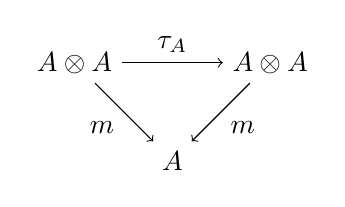
\begin{tikzpicture}[node distance = 5em]
   \node (AA1) {$A \otimes A$};
   \node[below right of = AA1] (A) {$A$};
   \node[above right of = A] (AA2) {$A \otimes A$};
   \draw[->] (AA1) to node[above] {$\tau_A$} (AA2);
   \draw[->] (AA1) to node[below left] {$m$} (A);
   \draw[->] (AA2) to node[below right] {$m$} (A);
  \end{tikzpicture}
 \end{center}
\end{definition}


\begin{remark}
 We will often just refer to a $k$-algebra $(A,m,u)$ by $A$ without explicitely mentioning $m$ and $u$. If necessary we will then refer to the multiplication by $m_A$ and the unit by $u_A$.
\end{remark}


\begin{remark}
 Definition \ref{defi: algebras via diagrams} is equivalent to the usual definition of a $k$-algebra, namely a $k$-vector space $A$ together with a bilinear map $\hat{m} \colon A \times A \to A, (a,b) \mapsto a \cdot b$ which is associative in the sense that $(a \cdot b) \cdot c = a \cdot (b \cdot c)$ for all $a,b,c \in A$, and such that a unit $1 \in A$ exists, i.e.\ an element for which $1 \cdot a = a \cdot 1 = a$ for every $a \in A$.
 
 Given a $k$-algebra in the usual sense the multiplication $\hat{m}$ corresponds to a linear map $m \colon A \otimes A \to A, a \otimes b \mapsto a \cdot b$, and that $m$ satisfies the associativity axiom is equivalent to $\hat{m}$ being associative. That a linear map $u \colon k \to A$ satisfies the unit axiom is equivalent to $u(1)$ being a unit in $A$. That $(A,\hat{m})$ is commutative is then also equivalent to $(A,m,u)$ being commutative.
 
 We will use both definitions, depending on which is more useful in a given situation, and switch between them if necessary.
\end{remark}


\begin{example}
 Let $G$ be any group. Then the \emph{group algebra} $k[G]$ is defined by the underlying vector space being $kG$, the free vector space with basis $G$, and the multiplication which arises from extending the multiplication of $G$ linearly, i.e.
 \[
  \left( \sum_{g \in G} \lambda_g g \right) \cdot \left( \sum_{h \in G} \mu_h h \right)
  = \sum_{g,h \in G} (\lambda_g \mu_h) (gh)
  = \sum_{g \in G} \left( \sum_{h \in G} \lambda_{gh^{-1}} \mu_h \right) g.
 \]
 The associativity of the multiplication can be checked by direct calculation. The unit of the group algebra $k[G]$ is given by the identity of the group $e \in G \subseteq k[G]$. The group algebra $k[G]$ is commutative if and only if $G$ is.
\end{example}


\begin{example}
 Let $A$ and $B$ be $k$-algebras. Then $A \otimes B$ carries the structure of a $k$-algebra via
 \[
  (a_1 \otimes b_1) \cdot (a_2 \otimes b_2)
  = (a_1 \cdot a_2) \otimes (b_1 \cdot b_2)
  \quad\text{for all $a_1, a_2 \in A$ and $b_1, b_2 \in B$}.
 \]
 Then $1_{A \otimes B} = 1_A \otimes 1_B$. The multiplication can also be expressed by the equality
 \[
  m_{A \otimes B} \colon
  A \otimes B \otimes A \otimes B
  \xrightarrow{\id_A \otimes\, \tau_{A,B} \otimes\, \id_A}
  A \otimes A \otimes B \otimes B
  \xrightarrow{m_A \otimes\, m_B}
  A \otimes B
 \]
 and the unit by
 \[
  u_{A \otimes B} \colon
  k
  \xrightarrow{\lambda \mapsto \lambda \otimes 1}
  k \otimes k
  \xrightarrow{u_A \otimes\, u_B}
  A \otimes B
 \]
\end{example}



\begin{definition}
 Let $A$ and $B$ be $k$-algebras. A linear map $f \colon A \to B$ is a \emph{homomorphism of $k$-algebras} if the following two diagrams commute:
 \begin{center}
  \raisebox{-\height}{
  \tikzsetnextfilename{homomorphism_of_algebras_multiplication}
  \begin{tikzpicture}[node distance = 5em]
   \node (AA) {$A \otimes A$};
   \node[right = 5em of AA] (BB) {$B \otimes B$};
   \node[below of = AA] (A) {$A$};
   \node[below of = BB] (B) {$B$};
   \draw[->] (AA) to node[above] {$f \otimes f$} (BB);
   \draw[->] (A) to node[below] {$f$} (B);
   \draw[->] (AA) to node[left] {$m_A$} (A);
   \draw[->] (BB) to node[right] {$m_B$} (B);
  \end{tikzpicture}}
  \hspace{0.5cm}
  \raisebox{-\height}{
  \tikzsetnextfilename{homomorphism_of_algebras_unit}
  \begin{tikzpicture}[node distance = 5em]
   \node (A) {$A$};
   \node[below right = of A] (k) {$k$};
   \node[above right = of k] (B) {$B$};
   \draw[->] (A) to node[above] {$f$} (B);
   \draw[->] (k) to node[below left] {$u_A$} (A);
   \draw[->] (k) to node[below right] {$u_B$} (B);
  \end{tikzpicture}}
 \end{center}
\end{definition}





\subsection{\texorpdfstring{$k$}{k}-coalgebras}


\begin{definition}
 A $k$-coalgebra is a tupel $(C,\Delta,\varepsilon)$ consisting of a $k$-vector space $C$, a linear map $\Delta \colon C \to C \otimes C$, called the \emph{comultiplication} and a linear map $\varepsilon \colon C \to k$, called the \emph{counit}, such that the following two diagrams commute:
 \begin{center}
  \tikzsetnextfilename{coassociativity_of_coalgebras}
  \begin{tikzpicture}[node distance = 5em]
   \node (C) {$C$};
   \node[right = 7em of C] (CC1) {$C \otimes C$};
   \node[below of = C] (CC2) {$C \otimes C$};
   \node[below of = CC1] (CCC) {$C \otimes C \otimes C$};
   \draw[->] (C) to node[above] {$\Delta$} (CC1);
   \draw[->] (C) to node[left] {$\Delta$} (CC2);
   \draw[->] (CC1) to node[right] {$\id_C \otimes\, \Delta$} (CCC);
   \draw[->] (CC2) to node[below] {$\Delta \otimes \id_C$} (CCC);
  \end{tikzpicture}
  \quad
  \tikzsetnextfilename{counit_of_coalgebras}
  \begin{tikzpicture}[node distance = 3em]
   \node (middle) {$ $};
   \node[above of = middle] (CC) {$C \otimes C$};
   \node[left = 5em of middle] (kC) {$k \otimes C$};
   \node[right = 5em of middle] (Ck) {$C \otimes k$};
   \node[below of = middle] (C) {$C$};
   \draw[->] (CC) to node[above left] {$\varepsilon \otimes \id_C$} (kC);
   \draw[->] (CC) to node[above right] {$\id_C \otimes \, \varepsilon$} (Ck);
   \draw[->] (C) to node[right] {$\Delta$} (CC);
   \draw[->] (C) to node[below left]  {$1 \otimes \id_C$} (kC);
   \draw[->] (C) to node[below right] {$\id_C \otimes\, 1$} (Ck);
  \end{tikzpicture}
 \end{center}
 The commutativity of the left diagram is the \emph{coassociativity axiom} and the commutativity of the right diagram is the \emph{counit axiom}. The coalgebra $(C, \Delta, \varepsilon)$ is called \emph{cocommutative} if the following diagram commutes:
 \begin{center}
  \tikzsetnextfilename{cocommutativity_of_coalgebras}
  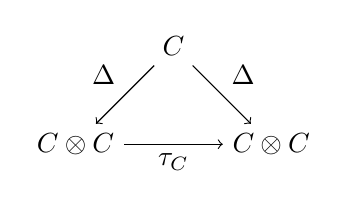
\begin{tikzpicture}[node distance = 5em]
   \node (CC1) {$C \otimes C$};
   \node[above right of = CC1] (C) {$C$};
   \node[below right of = C] (CC2) {$C \otimes C$};
   \draw[->] (CC1) to node[below] {$\tau_C$} (CC2);
   \draw[->] (C) to node[above left] {$\Delta$} (CC1);
   \draw[->] (C) to node[above right] {$\Delta$} (CC2);
  \end{tikzpicture}
 \end{center}
\end{definition}


\begin{examples}
 \begin{enumerate}[leftmargin=*]
  \item
   Let $C$ be a $k$-vector space and $(x_i)_{i \in I}$ a basis of $V$. Then $V$ carries the structure of a $k$-coalgebra via the comultiplication $\Delta \colon C \to C \otimes C$ defined by
   \[
    \Delta(x_i) \coloneqq x_i \otimes x_i \quad \text{for every $i \in I$}
   \]
   and the counit $\varepsilon \colon C \to k$ defined by
   \[
    \varepsilon\left( \sum_{i \in I} \lambda_i x_i \right) \coloneqq \sum_{i \in I} \lambda_i.
   \]
   To see that $\Delta$ is coassociative notice that for every $i \in I$
   \begin{align*}
     ((\id_C \otimes\, \Delta) \circ \Delta)(x_i)
     &= (\id_C \otimes\, \Delta)(x_i \otimes x_i)
     = x_i \otimes x_i \otimes x_i \\
     &= (\Delta \otimes \id_C)(x_i \otimes x_i)
     = ((\Delta \otimes \id_C) \circ \Delta)(x_i).
   \end{align*}
   To notice that $\varepsilon$ is a counit notice that for every $i \in I$
   \[
     ((\varepsilon \otimes \id_C) \circ \Delta)(x_i)
     = (\varepsilon \otimes \id_C)(x_i \otimes x_i)
     = 1 \otimes x_i
     = (1 \otimes \id_C)(x_i)
   \]
   and similarly $(\id_C \otimes\, \varepsilon) \circ \Delta = \id_C \otimes\, 1$.
   
  \item
   At a special case of the above example it follows that for any group $G$ the group algebra $k[G]$ also carries the structure of a $k$-coalgebra via the comultiplication $\Delta \colon k[G] \to k[G] \otimes k[G], g \mapsto g \otimes g$ and counit $\varepsilon \colon k[G] \to k, \sum_{g \in G} \lambda_g g \mapsto \sum_{g \in G} \lambda_g$.
 \end{enumerate}
\end{examples}


\begin{example}
 If $C$ and $D$ are $k$-coalgebras then $C \otimes D$ is a also a $k$-coalgebra via the comultiplication
 \[
  \Delta_{C \otimes D} \colon
  C \otimes D
  \xrightarrow{\Delta_C \otimes \Delta_D}
  C \otimes C \otimes D \otimes D
  \xrightarrow{\id_C \otimes \tau_{C,D} \otimes\, \id_C}
  C \otimes D \otimes C \otimes D
 \]
 and the counit
 \[
  \varepsilon_{C \otimes D} \colon
  C \otimes D
  \xrightarrow{\varepsilon_C \otimes\, \varepsilon_D}
  k \otimes k
  \xlongrightarrow{\lambda \otimes \mu \mapsto \lambda \mu}
  k.
 \]
\end{example}


\begin{definition}
 Let $C$ and $D$ be $k$-coalgebras. A linear map $f \colon C \to D$ is a homomorphism of $k$-coalgebras if the following diagrams commute:
 \begin{center}
  \raisebox{-\height}{
  \tikzsetnextfilename{homomorphism_of_coalgebras_comultiplication}
  \begin{tikzpicture}[node distance = 5em]
   \node (C) {$C$};
   \node[right = 5em of C] (D) {$D$};
   \node[below of = C] (CC) {$C \otimes C$};
   \node[below of = D] (DD) {$D \otimes D$};
   \draw[->] (C) to node[above] {$f$} (D);
   \draw[->] (CC) to node[below] {$f \otimes f$} (DD);
   \draw[->] (C) to node[left] {$\Delta_C$} (CC);
   \draw[->] (D) to node[right] {$\Delta_D$} (DD);
  \end{tikzpicture}}
  \hspace{0.5cm}
  \raisebox{-\height}{
  \tikzsetnextfilename{homomorphism_of_coalgebras_counit}
  \begin{tikzpicture}[node distance = 5em]
   \node (C) {$C$};
   \node[below right = of C] (k) {$k$};
   \node[above right = of k] (D) {$D$};
   \draw[->] (C) to node[above] {$f$} (D);
   \draw[->] (C) to node[below left] {$\varepsilon_C$} (k);
   \draw[->] (D) to node[below right] {$\varepsilon_D$} (k);
  \end{tikzpicture}}
 \end{center}
\end{definition}






\chapter{Schur’s Lemma}
Unless otherwise noted $k$ always is some arbitrary field. Whenever we talk about a ring (resp.\ $k$-algebra) we always mean an associative and unitary one, and homomorphisms of rings (resp.\ $k$-algebras) are required to respect the unit. We assume that the reader is familiar with the definition of a module over a ring notion of a submodules. By an (left) $R$-module $M$ over a ring $R$ we always mean an unitial module, i.e.\ $1 \cdot m = m$ for every $m \in M$.





\section{Classic version}


\begin{definition}
 Let $M$ be a module over a ring $R$. Then $M$ is called \emph{simple} or \emph{irreducible} if $M$ contains precisely two sumbodules. Equivalently $M$ in nonzero and its only submodules are the \emph{trivial} ones, namely $0$ and $M$ itself.
\end{definition}


\begin{lemma}[Schur] \label{lem: Schur general part about skew field}
 Let $R$ be a ring and $M$ a simple module over $R$. Then any endomorphism of modules $f \colon M \to M$ is either zero or an isomorphism. In particular $\End_R(M)$ is a skew field.
\end{lemma}
\begin{proof}
 As $M$ is nonzero $f$ cannot be zero and an isomorphism at the same time. If $f \neq 0$ then $\ker f$ is a proper submodule of $M$ and $\im f$ is a nonzero submodule of $M$, so $\ker f = 0$ and $\im f = M$ because $M$ is simple.
\end{proof}


\begin{corollary}
 Let $M$ be an $A$-module over a $k$-algebra $A$. Then $\End_A(M)$ is a division algebra over $k$.
\end{corollary}


\begin{lemma}\label{lem: algebraic elements over algebraically closed fields}
 Let $D$ be a division algebra over an algebraically closed field $k$. If $x \in D$ is algebraic over $k$ then already $x \in k$.
\end{lemma}
\begin{proof}
 Let $P \in k[T]$ be nonzero with $P(x) = 0$. W.l.o.g.\ $P$ can assumed to be monic. Because $k$ is algebraically closed there exist $\alpha_1, \dotsc, \alpha_r \in k$ with $P = \prod_{i=1}^r (x-\alpha_i)$. Because $0 = P(x) = c \prod_{i=1}^n (x-\alpha_i)$ and $D$ is a skew field it follows that $x = \alpha_i$ for some $i$ and therefore $x \in k$.
\end{proof}


\begin{corollary}
 Let $k$ be an algebraically closed field and $L$ a finite-dimensional division algebra over $k$. Then $L = k$.
\end{corollary}
\begin{proof}
 Let $x \in L$. Because $L$ is finite-dimenisonal over $k$ there exists some $n \geq 1$ such that $1, x, x^2, \dotsc, x^n$ are linearly dependent over $k$. Therefore there exist some $a_0, a_1, \dotsc, a_n \in k$ such that $a_0 + a_1 x + \dotsb + a_n x^n = 0$ is a non-trivial linear combination. Then $P = \sum_{i=0}^n a_i T^i \in k[T]$ is nonzero with $P(x) = 0$, so $x$ is algebraic over $k$. From Lemma~\ref{lem: algebraic elements over algebraically closed fields} it follows that $x \in k$.
\end{proof}


\begin{corollary}[Schur, classic Version] \label{cor: classic Schur}
 Let $k$ be an algebraically closed field and $M$ a simple $A$-module for a $k$-algebra $A$. If $M$ is finite-dimensional over $k$ then $\End_A(M) = k$, i.e.\ every module endomorphism of $M$ is given by multiplication with a scalar.
\end{corollary}


\begin{corollary}
 Let $\g$ be a Lie algebra over an algebraically closed field $k$ and $V$ a irreducible and finite-dimensional representation of $\g$. Then $\End_\g(V) = k$, i.e.\ every endomorpism of $V$ as a representation of $\g$ is given by an multiplication with some scalar.
\end{corollary}
\begin{proof}
 Take $V$ as a simple module over the universal enveloping algebra $\Ue(\g)$ and apply Corollary~\ref{cor: classic Schur}.
\end{proof}





\section{Generalization by Dixmier}


\begin{definition}
 Let $V$ be a vector space over a field $k$. An endomorphism $\varphi \in \End_k(V)$ is called \emph{algebraic} over $k$ there exists some nonzero polynomial $P \in k[T]$ mit $P(\varphi) = 0$.
\end{definition}


\begin{lemma}\label{lem: algebraic endomorphisms over algebraically closed fields}
 Let $k$ be an algebraically closed field, $V$ a vector space over $k$ and $D \subseteq \End_k(V)$ a division algebra over $k$. If $\varphi \in D$ is algebraic over $k$ then $\varphi = \alpha \id_V$ for some $\alpha \in k$.
\end{lemma}
\begin{proof}
 This follows directly from Lemma~\ref{lem: algebraic elements over algebraically closed fields}.
\end{proof}


\begin{corollary}\label{cor: Schur generally needs only algebraic endomorphisms}
 Let $k$ be an algebraically closed field, $A$ a $k$-algebra and $M$ a simple $A$-module. If $\varphi \in \End_A(M)$ is algebraic then $\varphi = \alpha \id_M$ for some $\alpha \in k$.
\end{corollary}
\begin{proof}
 This follows directly from Lemma~\ref{lem: algebraic endomorphisms over algebraically closed fields} because $\End_A(M) \subseteq \End_k(M)$ is a division algebra over $k$ by Lemma~\ref{lem: Schur general part about skew field}.
\end{proof}


The following Proposition traces back to \cite{Dixmier}. (At least this is what I found on the web --- I could not find the original article, nor would I be able to read it (as it was apparently written in French)).


\begin{proposition}[Dixmier]\label{prop: Dixmier}
 Let $M$ be a simple $A$-module for a $k$-algebra $A$, such that $\dim_k M > \card k$. Then every $\varphi \in \End_A(M)$ is algebraic over $k$.
\end{proposition}
\begin{proof}
 Suppose that there exists some $\varphi \in \End_A(M)$ which is not algebraic over $k$. Then the kernel of the map
 \[
  \iota \colon k[T] \to \End_A(M), \quad P \mapsto P(\varphi)
 \]
 is zero, hence $\iota$ is an inclusion of $k[T]$ into $\End_A(M)$, which is a skew field by Lemma \ref{lem: Schur general part about skew field}. It follows That $\iota$ can be extended to a well-defined inclusion
 \[
  \theta \colon k(T) \to \End_A(M), \quad \frac{P}{Q} \mapsto P(\varphi) Q(\varphi)^{-1}.
 \]
 Hence $M$ carries the structure of a $k(T)$-vector space with
 \[
  \frac{P}{Q} \cdot m = P(\varphi)Q(\varphi)^{-1}(m)
  \quad \text{for every $\frac{P}{Q} \in k(T)$ and $m \in M$}.
 \]
 
 As $M$ is a nonzero $k(T)$-vector space it follows that $\dim_k M \geq \dim_k k(T)$. To see this notice that if $L/k$ is any field extension and $V$ a nonzero $L$-vector space then there exists an inclusion $L \inc V$ of $L$-vector spaces. This is then also an inclusion of $k$-vector spaces, which is why $\dim_k V \geq \dim_k L$. The statement follows with $L = k(T)$ and $V = M$. (This is a straightforward generalization of the fact that every complex nonzero vector space is at least twodimensional as a real vector space.) Since $(1/(T-a))_{a \in k}$ is a familiy of elements of $k(T)$ which is linearly independent over $k$ it also follows that $\dim_k k(T) \geq \card k$.

 Putting the above observations together it follows that
 \[
  \dim_k M \geq \dim_k k(T) \geq \card k,
 \]
 contradicting the assumption that $\card k > \dim_k M$.
\end{proof}


\begin{corollary}\label{cor: Dixmier algebraically closed}
 Let $k$ be an algebraically closed field, $A$ a $k$-algebra and $M$ a simple $A$-module. If $\card k > \dim_k M$ then $\End_A(M) = k$.
\end{corollary}
\begin{proof}
 This is a combination of Corollary \ref{cor: Schur generally needs only algebraic endomorphisms} and Proposition \ref{prop: Dixmier}.
\end{proof}


\begin{corollary}
 Let $\g$ be a Lie algebra over an algebraically closed field $k$ and $V$ an irreducible representation of $\g$ with $\card k > \dim_k V$. Then $\End_\g(V) = k$.
\end{corollary}
\begin{proof}
 Take $V$ as a simple module over the universal enveloping algebra $\Ue(\g)$ and apply Corollary \ref{cor: Dixmier algebraically closed}.
\end{proof}


\begin{example}
 Let $\g$ be complex Lie algebra and $V$ an irreducible representation of $\g$ of countable dimension. Then $\End_\g(V) = \Cbb$.
\end{example}


\begin{remark}
 The requirement that $\card k > \dim_k M$ in Corollary \ref{cor: Dixmier algebraically closed} can not be dropped without adding some other restraints. To see this take $k \coloneqq \overline{\Q}$ as well as $A = M = \overline{\Q}(T)$. Then $\dim_k M = \card k$ and $\End_A(M) = \End_{\overline{\Q}(T)}(\overline{\Q}(T)) = \overline{\Q}(T)$.
\end{remark}





\section{Generalizaton by Quillen}


The following Proposition is due to \cite{Quillen}.


\begin{proposition}[Quillen] \label{prop: Quillen}
 Let $k$ be a field and $A$ a filtered $k$-algebra, such that $\gr A$ is finitely generated and commutative as a $k$-algebra. If $M$ is a simple $A$-module then every $\varphi \in \End_A(M)$ is algebraic over $k$.
\end{proposition}


\begin{corollary}
 Let $\g$ be finite-dimensional Lie algebra over an algebraically closed field $k$ and $V$ as irreducible representation of $\g$. Then $\End_\g(V) = k$.
\end{corollary}
\begin{proof}
 Take $V$ as a simple module over the universal enveloping algebra $\Ue(\g)$. If $x_1, \dotsc, x_n$ is a $k$-basis of $\g$ then by the abstract version of the PBW theorem
 \[
  \gr \Ue(\g) \cong S(\g) \cong k[x_1, \dotsc, x_n].
 \]
 Applying Proposition~\ref{prop: Quillen} to $\Ue(\g)$ and $V$ the statement follows from Corollary~\ref{cor: Schur generally needs only algebraic endomorphisms}.
\end{proof}


































% Appendix about reductive Lie algebras


\backmatter
\printnoidxglossary[type=symbols]
\printindex
\printbibliography


\end{document}
